\documentclass[oneside, 11pt]{book}
\usepackage{lmodern}
\usepackage[english]{babel}
\usepackage[T1]{fontenc}
\usepackage[utf8]{inputenc}
\usepackage{mathtools}
\usepackage{amsmath}
\usepackage{amssymb}
\usepackage{mathrsfs}
\usepackage{silence} %per ocultar un warning
\WarningFilter{gensymb}{Not defining \perthousand}
\WarningFilter{gensymb}{Not defining \micro}
\usepackage{siunitx} %per unitats en el SI
\usepackage{gensymb} %per el simbol de graus celsius
\usepackage{enumitem} %perquè item sigui un punt rodó i no quadrat
\usepackage{tikz}
\usepackage{tikz-3dplot}
\usetikzlibrary{matrix}
\usetikzlibrary{3d}
\usetikzlibrary{shapes.geometric, arrows.meta, positioning}
\usepackage{xcolor}
\usepackage{booktabs} % Para líneas más elegantes en tablas
\usepackage{array} % Para columnas m{} centradas verticalmente
\usepackage[Lenny]{fncychap}
\usepackage{dirtytalk}%per les cometes

\usepackage{etoolbox}

\makeatletter
\patchcmd{\@makechapterhead}
  {\vspace*{50\p@}} % valor por defecto típico en fncychap
  {\vspace*{-28\p@}} %  espai entre chapter i principi pàgina
  {}{}
\makeatother
 
\usepackage{longtable}
\usepackage[titles]{tocloft} % Paquete para modificar el índice


\usepackage{multirow}
\sisetup{output-decimal-marker = {.}, locale = US}
\usepackage{graphicx,wrapfig}
\usepackage[hypcap=false]{caption}
\usepackage[autostyle]{csquotes} % per fer quotes

\usepackage{pdflscape}
\usepackage{fancyhdr}
\usepackage{geometry}
\usepackage{subcaption}
\captionsetup[subfigure]{list=false}
\usepackage{footnote}
\usepackage{tabularx}
\usepackage{tcolorbox}
\tcbuselibrary{breakable}
\usepackage{cancel} %per taxar una equació
\setlength{\parindent}{0pt}  % sense sangria
\setlength{\parskip}{7pt} %espai entre paràgrafs
\ChNameVar{\fontsize{20}{60}\selectfont\fontseries{bx}\fontfamily{cmr}}
\ChNumVar{\fontsize{50}{100}\selectfont\fontfamily{cmr}}
\pagestyle{fancy}
\geometry{a4paper,left=25mm,right=25mm,headheight=2cm, bottom=0cm}
\setlength{\footskip}{1.5cm} %moure el numero de peu de pagina
\usepackage{setspace}
\setstretch{1.1} %espai entre linies de text
\addtolength{\textheight}{-60pt}
\addtolength{\topmargin}{-25pt} %margen superior
\usepackage{imakeidx}
\renewcommand{\headrulewidth}{0pt}
\usepackage{makecell}
\renewcommand\theadalign{bc}
\renewcommand\theadfont{\bfseries}
\renewcommand\theadgape{\Gape[4pt]}
\renewcommand\cellgape{\Gape[4pt]}
\makesavenoteenv{tabular}
\makesavenoteenv{table}
\usepackage{titlesec}
\titleformat{\paragraph}[block]{\normalfont\normalsize\bfseries}{\theparagraph}{1em}{} % per fer que el text d'un paragraph surti a sota i no al costat

\usepackage{listings}

% Definición de colores personalizados
\definecolor{codebg}{RGB}{252,252,252}
\definecolor{keywordblue}{RGB}{50,80,200}
\definecolor{stringgreen}{RGB}{30,140,30}
\definecolor{commentgray}{RGB}{130,130,130}

\lstdefinestyle{numpyStyle}{
    backgroundcolor=\color{codebg},
    basicstyle=\ttfamily\small,
    keywordstyle=\color{keywordblue}\bfseries,
    commentstyle=\color{commentgray}\itshape,
    stringstyle=\color{stringgreen},
    frame=single,
    rulecolor=\color{lightgray},
    language=Python,
    morekeywords={True, False, None},
    showstringspaces=false,
    breaklines=true,
    captionpos=b,
    aboveskip=10pt,
    belowskip=10pt,
}

\usepackage{hyperref}
\hypersetup{
    colorlinks=true,       % Colorea los enlaces (sin recuadros)
    linkcolor=blue,        % Color de los enlaces internos (índice)
    citecolor=green,        % Color de las referencias bibliográficas
    filecolor=blue,        % Color de los enlaces a archivos
    urlcolor=blue,         % Color de los enlaces web
}

\usepackage[
  backend=biber,
  style=numeric,
  sorting=none,
  doi=true,
  isbn=true,
  url=true,
  urldate=iso,
  backref=true,
  seconds=true,
  backrefstyle=three % compacta rangos consecutivos: 6–7, 11–12...
]{biblatex} %perquè surtin les pàgines on s'ha citat cada referència

\addbibresource{ref.bib} %posar el nom del document on hi ha les referencies 

\fancyhead{}

\pretocmd{\tableofcontents}{%
  \clearpage
  \pagestyle{empty}%
  \addtocontents{toc}{\protect\thispagestyle{empty}}%
}{}{}
\apptocmd{\tableofcontents}{%
  \clearpage
  \pagestyle{fancy}%
}{}{}

\pagenumbering{arabic} %per què comenci a contar les pàgines des d'aquí
\setcounter{page}{-6} %sino no funciona la bibliografia, aixo fa que intro comenci a 1 i no a 8

\makeatletter
\let\oldthebibliography=\thebibliography
\let\endoldthebibliography=\endthebibliography
\renewenvironment{thebibliography}[1]
  {\oldthebibliography{#1}
   \setlength{\itemsep}{4pt}  % Espacio entre referencias
   \setlength{\parskip}{0pt}
   \setlength{\parsep}{0pt}}
  {\endoldthebibliography}
\makeatother

\setcounter{secnumdepth}{4}  % perque es vegi fins a 1.1.1.1 al cos del document
\setcounter{tocdepth}{4}  % perque es vegi fins a 1.1.1.1 a l'index

\setlength{\cftbeforefigskip}{9pt} % espai entre figures a la list of figures

% Colores personalizados
\definecolor{energycolor}{RGB}{213,232,213}
\definecolor{momentumcolor}{RGB}{213,232,213}
\definecolor{pressurecolor}{RGB}{255,220,210}
\definecolor{shearcolor}{RGB}{220,225,255}


\newcommand{\chapterlink}[2]{%
  \hyperref[#1]{\textbf{\textcolor{cyan}{#2}}}%
} %per el summary dels chapters


% Configure description environment
\setlist[description]{%
  leftmargin=0cm,     % Align labels 
  labelwidth=\dimexpr0.8cm\relax, % Match label width to leftmargin
  labelsep=0.2cm,         % No space between label and text
  itemindent=0pt,       % No extra indent for first line
  font=\normalfont,     % Normal font for label (adjust if needed)
  style=standard        % Standard description style
}

\makeatletter
\def\@endpart{} % Elimina el salt de pàgina després de \part
\makeatother


\begin{document}

\renewcommand{\headrulewidth}{0pt} %No Horizontal Line at top

\thispagestyle{empty}
\definecolor{colorTFG}{RGB}{79,129,189}
\begin{picture}(\paperheight, \paperwidth)(80,-670)
	\setlength\unitlength{1mm}
	\put(28,-13){\makebox(0,0)[lt]{
\includegraphics[height=21mm]{Figures/logo.pdf}}}
	\put(37,-60){\makebox(0,0)[lt]{\LARGE\sffamily\bfseries{\MakeUppercase{Master's Thesis}}}}
	\put(189,-93){\makebox(0,0)[rt]{\parbox{115mm}{\raggedleft\LARGE\sffamily\bfseries\MakeUppercase{PARAMETER ESTIMATION AND SKY LOCALIZATION OF LENSED IMAGE PAIRS OF BINARY BLACK HOLE MERGERS}}}}
	\put(37,-146){\makebox(0,0)[lb]{\LARGE\sffamily\bfseries{Xavier Garcia Sàbat}}}
	\put(37,-165){\makebox(0,0)[lb]{\large\sffamily\bfseries{Master's Degree in Advanced Physics and Applied Mathematics}}}
	\put(37,-175){\makebox(0,0)[lb]{\large\sffamily\bfseries{Centre for Postgraduate Studies}}}	
	\put(37,-201){\makebox(0,0)[lb]{\sffamily\bfseries{Academic Year 2025-26}}}
\end{picture}

\newpage
\vspace*{\fill}
	\begin{center}
		\thispagestyle{empty}
	\end{center}
\vspace*{\fill}
\newpage

\thispagestyle{empty}
\begin{picture}(\paperheight, \paperwidth)(80,-670)
	\setlength\unitlength{1mm}
	\put(37,-50){\makebox(0,0)[lt]{\parbox{145mm}{\raggedright\LARGE\sffamily\bfseries\MakeUppercase{PARAMETER ESTIMATION AND SKY LOCALIZATION OF LENSED IMAGE PAIRS OF BINARY BLACK HOLE MERGERS}}}}
	\put(37,-97){\makebox(0,0)[lb]{\LARGE\sffamily\bfseries{Xavier Garcia Sàbat}}}
	\put(37,-115){\makebox(0,0)[lb]{\Large\sffamily\bfseries{Master's Thesis}}}
	\put(37,-127){\makebox(0,0)[lb]{\Large\sffamily\bfseries{Centre for Postgraduate Studies}}}
	\put(37,-139){\makebox(0,0)[lb]{\Large\sffamily\bfseries{University of the Balearic Islands}}}
	\put(37.6,-150){\makebox(0,0)[lb]{\sffamily\bfseries{Academic Year 2025-26}}}
	\put(37,-170){\makebox(0,0)[lb]{\sffamily{Keywords:}}}
	\put(37,-177){\makebox(0,0)[lt]{\parbox{145mm}{\raggedright\sffamily{Gravitational waves, Strong gravitational lensing, Parameter estimation, Sky localization, Binary black holes, LIGO}}}}
	\put(37,-211){\makebox(0,0)[lb]{\large\sffamily\emph{Thesis Supervisor's Name: David Benjamin Keitel}}}
\end{picture}

\newpage

\thispagestyle{empty} %to hide page number
\vspace*{\fill}
\begin{center}
\hrule
\vspace{1.5em}

\textbf{Aquest treball de fi de màster està subjecte a la llicència: ``\href{https://creativecommons.org/licenses/by-nc-nd/4.0/}{Creative Commons: Reconeixement - NoComercial - SenseObraDerivada (\textit{by-nc-nd})}''}

\vspace{1em}

\textbf{Este trabajo de fin de máster está sujeto a la licencia: ``\href{https://creativecommons.org/licenses/by-nc-nd/4.0/}{Creative Commons: Reconocimiento - NoComercial - SinObraDerivada (\textit{by-nc-nd})}''}

\vspace{1em}

\textbf{This master's thesis is licensed under the: ``\href{https://creativecommons.org/licenses/by-nc-nd/4.0/}{Creative Commons: Attribution - NonCommercial - NoDerivatives (\textit{by-nc-nd})}''}

\vspace{1.5em}


\includegraphics[width=5cm]{Figures/cc-by-nc-nd.png}
\end{center}


%====================================
\frontmatter % numeros romans índex
\pagenumbering{Roman}
\fontfamily{cmr}\selectfont

\chapter*{\textbf{Acknowledgments}}
\phantomsection
\addcontentsline{toc}{chapter}{Acknowledgments}



\newpage

\chapter*{\textbf{Summary}}
\phantomsection %perque funcioni l'hyperref
\addcontentsline{toc}{chapter}{Summary}

The structure of this thesis is organized as follows: 


\begin{description}[leftmargin=1cm]
  \item[\chapterlink{Introduction_to_General_Relativity}{Chapter 1: Introduction to general relativity.}] We give an overview of gravitational waves and then ... asmdosamc .... ofmwomo... cas,cs,c,spcs... kc comomaomc gives an overview of gravitational waves and then ... asmdosamc .... ofmwomo... cas,cs,c,spcs... kc comomaomc

  \item[\chapterlink{Gravitational-wave theory}{Chapter 2: Gravitational wave theory.}] gives an overview of gravitational waves and then ... asmdosamc .... ofmwomo... cas,cs,c,spcs... kc comomaomc gives an overview of gravitational waves and then ... asmdosamc .... ofmwomo... cas,cs,c,spcs... kc comomaomc
  \item[\chapterlink{Gravitational lensing}{Chapter 3: Gravitational lensing.}] gives an overview of gravitational waves and then ... asmdosamc .... ofmwomo... cas,cs,c,spcs... kc comomaomc gives an overview of gravitational waves and then ... asmdosamc .... ofmwomo... cas,cs,c,spcs... kc comomaomc

  \item[\chapterlink{Conclusions}{Chapter 4: Conclusions.}] introduces the ..
  \item[\chapterlink{Glossary}{Appendix A: Glossary.}] introduces the ..

  \item[\chapterlink{Proofs and derivations}{Appendix B: Proofs and derivations.}] introduces the ...

  \item[\chapterlink{Parameters_CBC_appendix}{Appendix C: Parameters of Compact Binary Coalescences.}] introduces the ...
  \item[] 
  \item[\chapterlink{Reproducibility tutorial}{Appendix D: Reproducibility tutorial.}] introduces the ...

  

\end{description}


\newpage


\renewcommand{\contentsname}{\textbf{Contents}}
\phantomsection %perque funcioni l'hyperref
\addcontentsline{toc}{chapter}{\textbf{Contents}}

\tableofcontents


\listoffigures %perquè a la biblio no surti que les fotos s'han citat a la list of figures
\phantomsection %perque funcioni l'hyperref
\addcontentsline{toc}{chapter}{List of Figures}
\newpage

\section*{\textbf{Abbreviations}}
\phantomsection%perque funcioni l'hyperref
\addcontentsline{toc}{chapter}{Abbreviations}

\newcolumntype{R}[1]{>{\raggedleft\bfseries}p{#1}}  % Right-align in fixed width
\newcolumntype{L}[1]{p{#1}}                         % Left-align in fixed width

\begin{center}
\begin{tabular}{R{5cm} L{10cm}}

BBH & \textbf{B}inary \textbf{B}lack \textbf{H}ole \\
BH & \textbf{B}lack \textbf{H}ole \\
BNS & \textbf{B}inary \textbf{N}eutron \textbf{S}tar \\
CBC & \textbf{C}ompact \textbf{B}inary \textbf{C}oalescence \\
CE & \textbf{C}osmic \textbf{E}xplorer \\
CW & \textbf{C}ontinuous gravitational \textbf{W}ave \\
EFE & \textbf{E}instein \textbf{F}ield \textbf{E}quations \\
EM & \textbf{E}lectro\textbf{m}agnetic \\
EOB & \textbf{E}ffective \textbf{O}ne \textbf{B}ody \\
EPL & \textbf{E}lliptical \textbf{P}ower \textbf{L}aw \\
ET & \textbf{E}instein \textbf{T}elescope \\
FLRW & \textbf{F}riedmann-\textbf{L}ema\^{i}tre-\textbf{R}obertson-\textbf{W}alker \\
GR & \textbf{G}eneral \textbf{R}elativity \\
GW & \textbf{G}ravitational \textbf{W}ave \\
GWTC & \textbf{G}ravitational-\textbf{W}ave \textbf{T}ransient \textbf{C}atalog \\
HLV & \textbf{H}anford-\textbf{L}ivingston-\textbf{V}irgo (three-detector network) \\
HPC & \textbf{H}igh \textbf{P}erformance \textbf{C}omputing \\
IGWN & \textbf{I}nternational \textbf{G}ravitational-\textbf{W}ave Observatory \textbf{N}etwork \\
IMR & \textbf{I}nspiral-\textbf{M}erger-\textbf{R}ingdown \\
IR1 & \textbf{I}ntermediate \textbf{R}un \textbf{1} (between O4 and O5) \\
LHO & \textbf{L}IGO \textbf{H}anford \textbf{O}bservatory \\
LIGO & \textbf{L}aser \textbf{I}nterferometer \textbf{G}ravitational-wave \textbf{O}bservatory \\
LISA & \textbf{L}aser \textbf{I}nterferometer \textbf{S}pace \textbf{A}ntenna \\
LLO & \textbf{L}IGO \textbf{L}ivingston \textbf{O}bservatory \\
LSC & \textbf{L}IGO \textbf{S}cientific \textbf{C}ollaboration \\
LVK & \textbf{L}IGO-\textbf{V}irgo-\textbf{K}AGRA \\
MC & \textbf{M}onte \textbf{C}arlo \\
MCMC & \textbf{M}arkov \textbf{C}hain \textbf{M}onte \textbf{C}arlo \\
NFW & \textbf{N}avarro-\textbf{F}renk-\textbf{W}hite \\
NR & \textbf{N}umerical \textbf{R}elativity \\
NS & \textbf{N}eutron \textbf{S}tar \\
NSBH & \textbf{N}eutron \textbf{S}tar-\textbf{B}lack \textbf{H}ole (binary) \\
O1, O2, O3, O4, O5 & \textbf{O}bservation run 1, 2, 3, 4, 5 of the LVK network \\
PE & \textbf{P}arameter \textbf{E}stimation \\
PN & \textbf{P}ost-\textbf{N}ewtonian \\
PSD & \textbf{P}ower \textbf{S}pectral \textbf{D}ensity \\
SGWB & \textbf{S}tochastic \textbf{G}ravitational \textbf{W}ave \textbf{B}ackground \\
SIE & \textbf{S}ingular \textbf{I}sothermal \textbf{E}llipsoid \\
SIS & \textbf{S}ingular \textbf{I}sothermal \textbf{S}phere \\
SNR & \textbf{S}ignal-to-\textbf{N}oise \textbf{R}atio \\
TDI & \textbf{T}ime \textbf{D}elay \textbf{I}nterferometry \\
TT & \textbf{T}ransverse-\textbf{T}raceless \\
WD & \textbf{W}hite \textbf{D}warf \\



\end{tabular}
\end{center}



\newpage

\pagenumbering{arabic}
\mainmatter % numeros normals índex

\part{Theoretical introduction}
\vspace{4cm}
The first three chapters provide the theoretical foundation of this thesis. Chapter~\ref{Introduction_to_General_Relativity} introduces 
general relativity, developing the mathematical framework of curved spacetime and the Einstein field equations. 
Chapter~\ref{Gravitational-wave theory} derives gravitational waves from the linearized field equations and describes the current network of interferometric detectors and the Bayesian parameter estimation framework. Chapter~\ref{ch:lensing} introduces gravitational lensing, develops the strong lensing formalism for gravitational waves, and motivates the joint analysis of lensed image pairs for sky localization.

\chapter{Introduction to General Relativity}
\label{Introduction_to_General_Relativity}

Nowadays, general relativity (GR) is fundamental to our understanding of modern astrophysics. Whether we’re studying black holes (BHs), quasars, or gravitational lensing, Einstein’s theory provides the essential framework. Efforts to detect gravitational waves (GWs) are a direct test of one of his key theoretical predictions. It marks a remarkable chapter in the story of one of the most influential equations of the 20th century.

\section{Motivation and Historical Background}

The centenary of GR marks not only one of the greatest theoretical advances in physics, but also the foundation of modern astrophysical exploration. From its inception in 1915, Einstein’s theory has evolved far beyond corrections to planetary orbits, becoming a central pillar in our understanding of the cosmos \cite{MaxPlanckChronology}.

\subsection{Key Historical Milestones}
\label{Key Historical Milestones}

\begin{itemize}
  \item \textbf{1905--1907:} Following his groundbreaking special relativity paper \cite{einstein1905originalpaper}, Einstein seeks a relativistic framework for gravitation, which results in the formulation of GR in 1915.
  
  \item \textbf{1916:} Within months, Karl Schwarzschild finds the first exact solution to Einstein's equations \cite{paperschwarzschild1916_pointmass}, revealing the theoretical existence of BHs, a concept reinforced in 1917 when Einstein applies his theory to cosmology.
  \item \textbf{1919:} Arthur Eddington’s eclipse expedition confirms the bending of starlight by the Sun’s gravity \cite{Eddingtonsexpedition}, providing one of the first key empirical validations of the theory. 
  \item \textbf{1927--1929:} Georges Lemaître and Edwin Hubble independently establish the expanding universe paradigm \cite{LemaitreHubble}, linking GR to the observable evolution of the cosmos.
  \item \textbf{1960s--1970s:} After decades of theoretical neglect, interest in GR resurges. Joseph Weber pioneers early experimental searches for GWs \cite{JosephWeber}, and the discovery of the Hulse-Taylor pulsar in 1974 offers indirect but compelling evidence that energy is indeed carried away by gravitational radiation.
  \item \textbf{1980s--1990s:} Interferometric efforts gain traction: the Max‑Planck Institute begins building early prototypes, leading to collaborations that produce GEO600 and pave the way for LIGO and Virgo \cite{upgradeofGEO600}.
  \item \textbf{2015--2017:} The detection of GW150914 by LIGO in September 2015 \cite{PrimeradeteccioGW150914}, publicly announced in February 2016, marks the first direct observation of GW, fulfilling a century-old prediction and inaugurating the era of gravitational-wave astronomy.
\end{itemize}

This historical path underscores GR's pivotal role beyond theoretical elegance.

\subsubsection{Einstein's journey to general relativity}
\label{Einstein's journey to general relativity}


Einstein's search for the accurate gravitational field equations unfolded over a series of crucial weekly submissions in November 1915 to the \href{https://en.wikipedia.org/wiki/Prussian_Academy_of_Sciences}{Prussian Academy of Sciences} \cite{EinsteinsjourneyPrussian}.

On each of the four Thursdays in November 1915, Einstein presented groundbreaking work that ultimately led to the final form of GR:

\begin{itemize}
    \item \textbf{November 4, 1915}: Einstein discards the Entwurf theory\footnote{The \enquote{Entwurf theory} represented Einstein's formulation of GR from spring 1913 until October 1915, developed in collaboration with Marcel Grossmann \cite{Entwurftheory}.} and submits a new paper to the Prussian Academy, introducing an early version of what would become the General Theory of Relativity. The paper was titled \enquote{On the General Theory of Relativity} \cite{Einstein1915Nov4}.
    
    \item \textbf{November 11, 1915}: He submits an addendum titled \enquote{On the General Theory of Relativity (Addendum)} \cite{Einstein1915bNov11}, proposing the idea that macroscopic matter might be fundamentally explainable through electromagnetic phenomena.
    
    \item \textbf{November 18, 1915}: In a new paper titled \enquote{Explanation of the Perihelion Motion of Mercury from the General Theory of Relativity} \cite{Einstein1915cNov18}, Einstein demonstrates that his equations predict the correct value of Mercury’s perihelion shift (45'' per century), aligning with astronomical observations, unlike the prior estimate of 18''.
    
    \item \textbf{November 25, 1915}: Einstein delivers the final and complete formulation of his theory, in the paper \enquote{The Field Equations of Gravitation} \cite{Einstein1915dNov25}, where he proposes three distinct versions of the gravitational field equations, two of which are generally covariant.
\end{itemize}


\subsection{Equivalence principle}

The equivalence principle played a central role in the development of GR. The idea that a freely falling observer does not locally experience gravity led Einstein to what he later described as ``the happiest thought of my life'':

\enquote{Then there occurred to me the `glückichste Gedanke meines Lebens,' the happiest thought of my life \cite{Happiestthoughtofmylife}, in the following form. The gravitational field has only a relative existence in a way similar to the electric field generated by magnetoelectric induction. Because for an observer falling freely from the roof of a house there exists, at least in his immediate surroundings, no gravitational field. Indeed, if the observer drops some bodies then these remain relative to him in a state of rest or of uniform motion, independent of their particular chemical or physical nature (in this consideration the air resistance is, of course, ignored). The observer therefore has the right to interpret his state as at rest} \footnote{As quoted in Pais (1982), p.~178 \cite{QuoteEinstein_Pais}.}


\subsubsection{The weak equivalence principle}

The origins of special relativity can be traced back to the 17\textsuperscript{th} century, when Galileo Galilei introduced what would later be known as the Principle of relativity. In a broader sense, the roots of GR also reach back to this period. Thinkers such as Galilei and Simon Stevin (1548-1620) began to recognize that the velocity reached by freely falling objects is independent of their mass, a realization that contradicted both everyday intuition and the Aristotelian view of physics \cite{LlibreBertJanssen}.

A famous, though historically inaccurate, anecdote claims that Galileo dropped spheres of different masses from the Leaning Tower of Pisa to prove they would hit the ground simultaneously. In reality, Galileo derived his conclusions on free fall by rolling spheres down inclined planes, results which he presented in his 1590 manuscript De Motu \cite{DeMotuGalilei}.

The universality of free fall, the fact that the velocity of a freely falling object does not depend on its mass, reflects a striking feature of Newtonian mechanics: the equivalence between inertial mass $m_i$ and gravitational mass $m_g$, also called the weak equivalence principle.

In Newtonian theory, two distinct concepts of mass emerge in different contexts. The first is the inertial mass $m_i$, which appears in Newton’s second law as the constant of proportionality between the applied force $\vec{F}$ and the resulting acceleration $\vec{a}$:
\begin{equation}
    \vec{F}=m_i \ \vec{a} \ .
\end{equation}
Inertial mass represents how strongly an object resists changes in its velocity; in other words, how much it opposes acceleration.
On the other hand, gravitational mass refers to how an object engages in gravitational interactions with other masses in the universe.
The gravitational potential that one object generates and exerts on another is given by:
\begin{equation}
    V=\frac{G_N \ m_{\mathrm{g}} \ M_{\mathrm{g}}}{r} \ ,
\end{equation}
where $G_N$ is Newton's gravitational constant and $r$ is the distance between the two masses $m_g$ and $M_g$.

The fact that all objects fall at the same rate suggests a fundamental link between the two types of mass.  
Indeed, the motion of an object in free fall is governed by Newton's second law, where $\vec{F} = -m_g g \hat{e}_z$ is the Galilean gravitational force
\begin{equation}
    -m_{\mathrm{g}} g=m_{\mathrm{i}} \ddot{z} \ .
\end{equation}
In general, the solution to this equation takes the form:
\begin{equation}
    z(t)=-\frac{1}{2} \frac{m_{\mathrm{g}}}{m_{\mathrm{i}}} g t^2+v_0 t+z_0 \ ,
\end{equation}
where \( {v}_0 \) and \({z}_0 \) are integration constants determined by the initial conditions.  
However, to understand why two bodies with different masses, both inertial and gravitational, reach the ground at the same time when released under identical initial conditions, we must assume that:
\begin{equation}
    \frac{m_{\mathrm{g}}}{m_{\mathrm{i}}}=\text{constant} \ .
\end{equation}
At first glance, one might expect this ratio to vary depending on the material, for instance, that a steel ball might fall faster or slower than a wooden one.  
However, experiments show that the ratio $m_g / m_i$ is a universal constant (independent of the material), and can be set to 1 with an appropriate choice of units.

Indeed, a long history of experimental tests has confirmed the equivalence of inertial and gravitational mass with remarkable precision.  
In 1888, Hungarian physicist Baron Loránd von Eötvös (1848--1919) developed a torsion balance capable of detecting differences in the ratio $m_g / m_i$ between two test bodies \cite{The_Eötvös_Torsion_Balance}.  
He used Earth's gravity and its daily rotation as references to measure gravitational and inertial mass, respectively, and achieved a precision of:
\begin{equation}
\left| \frac{m_g - m_i}{m_g} \right| \sim 10^{-9}.
\end{equation}
In 1964, American physicist Robert Dicke (1916--1997) improved upon this method by using Earth's orbit around the Sun \cite{RobertDicketest}, reaching a precision of:
\begin{equation}
\left| \frac{m_g - m_i}{m_g} \right| < 10^{-11}.
\end{equation}
Currently, the weak equivalence principle has been tested in space with unprecedented precision, at the \(10^{-14}\) level, by the MicroSCOPE satellite mission, led by ONERA and CNES \cite{CNES_MICROSCOPE_eoportal, MicroSCOPEarxiv}.


\subsubsection{The strong equivalence principle}

Although Newtonian mechanics offered no fundamental reason for these two physical quantities to be equal, Einstein believed this could not be a mere coincidence; rather, it hinted at a deeper property of Nature.

The breakthrough came in 1907 when Einstein realized that an observer in free fall does not feel their own weight and might therefore conclude that they are in a region of space where no gravitational field is present. In fact, any object released by this observer during free fall would fall at the same rate as the observer, due to the universality of free fall. As a result, the observer would see the object floating next to them, as if both were drifting in interstellar space.

Thus, even though such an observer is not inertial in the Newtonian sense, someone falling freely in a uniform gravitational field could reasonably consider themselves to be at rest in a gravity-free environment.

\begin{center}
\begin{minipage}{0.9\textwidth}
\begin{center}
\setlength{\fboxsep}{7pt}
\setlength{\fboxrule}{0.75pt}
\fbox{%
  \parbox{0.95\textwidth}{%
    \textbf{Equivalence Principle} (for uniform gravitational fields): \textit{An observer in free fall within a constant gravitational field is equivalent to an inertial observer in the absence of gravity. It is impossible to distinguish between these two situations by means of physical experiments.}
  }%
}
\end{center}
\end{minipage}
\end{center}

Alternatively if we are in a laboratory on Earth, a mass that is released will fall, accelerating downward due to Earth's gravitational pull, at a rate of $g = 9.80665~\mathrm{m/s^2}$.

Let us now consider releasing the same object inside a rocket that is accelerating with a constant acceleration $a$, equal in magnitude to the gravitational acceleration $g$ on Earth.

In this scenario, the rocket’s floor accelerates upward and effectively moves toward the freely falling object. From the perspective of the observer inside the rocket, the object appears to accelerate downward toward the floor, just as it would under Earth's gravity. In both cases, the observed motion of the object relative to the floor is indistinguishable.

If the laboratory inside the rocket were completely enclosed and had no windows, the observer would have no way of telling whether the apparent acceleration was caused by a gravitational field (as on Earth) or by the rocket’s uniform acceleration through space.

Therefore, an observer undergoing constant acceleration, although not inertial in the Newtonian sense, could consider themselves at rest within an equivalent gravitational field.

\begin{center}
\begin{minipage}{0.9\textwidth}
\begin{center}
\setlength{\fboxsep}{7pt}
\setlength{\fboxrule}{0.75pt}
\fbox{%
  \parbox{0.95\textwidth}{%
    \textbf{Equivalence Principle} (for constant accelerations): \textit{An observer undergoing uniform acceleration is equivalent to an inertial observer in a uniform gravitational field. It is impossible to distinguish between these two situations through physical experiments.}
  }%
}
\end{center}
\end{minipage}
\end{center}


The problem we encounter is that the Equivalence principle no longer holds in the case of general gravitational fields, since the inhomogeneities of the field allow an observer to distinguish between being in free fall and being truly inertial in the absence of gravity\footnote{The Equivalence principle is only valid locally, that is, on small spatial or temporal scales.  
At larger scales, one can distinguish between gravity and acceleration through \href{https://en.wikipedia.org/wiki/Tidal_force}{tidal forces}, which arise due to the inhomogeneity of the gravitational field \cite{LlibreBertJanssen}.}. 

For example, in a radial gravitational field (such as the one produced by a spherically symmetric mass like the Earth), two freely falling objects do not follow parallel trajectories. Instead, they slowly move closer together as they fall toward the center of the field (see Fig. \ref{fig:earth_lab_frame}). 


\begin{figure}[h]
    \centering
    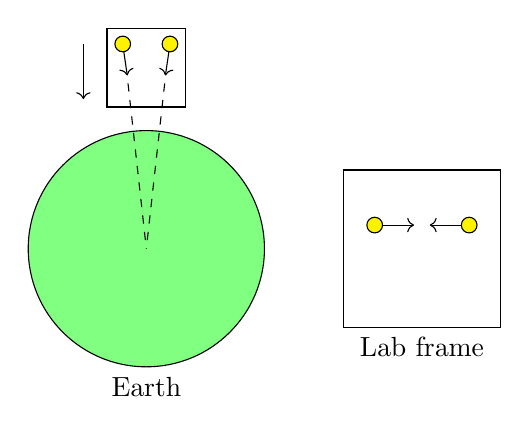
\begin{tikzpicture}

    % Diagrama de la Tierra
    \node[circle, draw, fill=green!50, minimum size=3cm, label=below:Earth] (earth) at (0,0) {};
    \draw[dashed] (-0.233,2.1) -- (0,0);
    \draw[dashed] (0.233,2.1) -- (0,0);
    \draw[->] (-0.8,2.6) -- (-0.8,1.9);
    \node[draw, minimum size=1cm] at (0,2.3) {};
    \node[circle, draw=black, fill=yellow, inner sep=2pt] at (-0.3,2.6) {};
    \node[circle, draw=black, fill=yellow, inner sep=2pt] at (0.3,2.6) {};
    \draw[->] (-0.286,2.5) -- (-0.242,2.2);
    \draw[->] (0.286,2.5) -- (0.242,2.2);

    % Diagrama del marco de laboratorio
    \node[rectangle, draw, minimum size=2cm] at (3.5,0) {};
    \node[circle,draw=black, fill=yellow, inner sep=2pt] at (2.9,0.3) {};
    \node[circle,draw=black, fill=yellow, inner sep=2pt] at (4.1,0.3) {};
    \draw[->] (3,0.3) -- (3.4,0.3);
    \draw[->] (4,0.3) -- (3.6,0.3);
    \node at (3.5,-1.25) {Lab frame};

    \end{tikzpicture}
    \caption{A simple non-local experiment: Two test particles, dropped in a radial gravitational field such as Earth's, follow slightly converging paths due to tidal effects. Although both particles are in free fall, they are attracted toward slightly different directions, each toward the Earth's center, causing them to slowly move closer. This convergence is not due to their mutual gravitational attraction, but rather to the non-uniformity of the field. This illustrates the presence of curvature through tidal forces. Original illustration based on the source: \cite{llibretongGR}.}
    \label{fig:earth_lab_frame}
\end{figure}



With sufficiently precise measurements, a free-falling observer could detect this effect and realize that they are in a real gravitational field.

However, tidal forces are negligible at small scales, since they are proportional to the gradient of the gravitational field.  
Therefore, at scales small enough for the field to appear locally uniform, tidal effects vanish, and the Equivalence principle becomes valid once again, though only locally.

\begin{center}
\begin{minipage}{0.9\textwidth}
\begin{center}
\setlength{\fboxsep}{7pt}
\setlength{\fboxrule}{0.75pt}
\fbox{%
  \parbox{0.95\textwidth}{%
    \textbf{Equivalence Principle} (general formulation): \textit{Free-falling observers in a gravitational field are locally indistinguishable from inertial observers. There are no local experiments that can differentiate between these two scenarios.}
    }
}
\end{center}
\end{minipage}
\end{center}


\subsubsection{Mathematical implications (local inertial frame)}


The local validity of the Equivalence principle implies that, in small regions, gravity can be eliminated through a suitable choice of coordinates, making spacetime appear flat (locally Minkowskian). 

Mathematically, at any point \( P \) in spacetime, it is possible to choose coordinates \( x'^\alpha \) such that the metric becomes locally flat:
\begin{equation}
g'_{\mu\nu}(x'_P) = \eta_{\mu\nu} \ ,
\end{equation}
where \( \eta_{\mu\nu} = \mathrm{diag}(-1, 1, 1, 1) \) is the Minkowski metric. This implies that spacetime is locally Minkowskian, though globally it may be curved due to gravitational inhomogeneities \cite{Llibrehartle2003gravity}.

Indeed, it is not possible to find coordinates in which \( g_{\mu\nu}= \eta_{\mu\nu} \)  everywhere. If such coordinates existed globally, the spacetime would be flat.

However, at any point \( P \), it is always possible to choose a coordinate system (normal coordinates) such that:
\begin{equation}
    g_{\mu \nu}^{\prime}\left(x_P^{\prime}\right)=\eta_{\mu \nu} \ ,\left.\quad \frac{\partial g_{\mu \nu}^{\prime}}{\partial x^{\prime \alpha}}\right|_{x=x_P}=0 \ .
\end{equation}
That is, the metric is locally flat at \( P \), and its first derivatives vanish. The curvature of spacetime is encoded in the second derivatives of the metric, which in general do not vanish \cite{llibretongGR}:
\begin{equation}
\partial_\lambda \partial_\rho g_{\mu\nu}(P) \neq 0 \ .
\end{equation}
A coordinate system that meets these two conditions at a point $P$ is referred to as a local inertial frame. Within a sufficiently small neighborhood of $P$, it mimics the behavior of an inertial frame in flat spacetime. Such frames can exist at any point, but always require a different coordinate system.

This local flatness underlies the geometric interpretation of gravity in GR: free particles follow geodesics of curved spacetime, and geodesic deviation leads to effects that mimic gravitational forces. In this framework, gravity is not a force but a consequence of curvature.


\section{The description of curved spacetime}


After his work on special relativity and learning about the mathematical structure introduced by Minkowski \cite{Minkowski}, Einstein realized that space-time itself possesses a geometry. Instead of thinking of space and time as separate and absolute entities, special relativity showed that they are part of a unified, four-dimensional space-time fabric. 

Before introducing gravity, it is crucial to recall this idea: space-time itself has a geometry. In special relativity, this geometry is flat (Minkowskian); however, the presence of mass and energy changes this picture.

To describe this curved geometry, Euclidean tools are no longer sufficient. Instead, we require a more general mathematical framework: Riemannian geometry, capable of capturing the curvature induced by mass and energy. In this section, we will extend that concept further.



\subsection{From euclidean to non-euclidean geometry}


The geometry most familiar to us, euclidean geometry, describes flat space. In this framework, parallel lines never meet, and the angles of a triangle always sum to 180 degrees. These properties stem from the foundational work of the Greek mathematician \href{https://en.wikipedia.org/wiki/Euclid}{Euclid}, who around 300 BC compiled much of the mathematical knowledge of his time in a 13-book series known as ``The Elements'' \footnote{For over two millennia, The Elements has served as the definitive reference on the geometry of flat spaces, so much so that this branch is often referred to as euclidean geometry. Since its first printed edition in Venice in 1482, The Elements has seen the publication of at least 1{,}000 editions, making it the second most published book in history, surpassed only by the Bible \cite{LlibreBertJanssen}.
} \cite{Elements}. In it, he formulated five postulates from which he derived hundreds of theorems, laying the groundwork for classical geometry. Among these, the fifth, the parallel postulate, stood out for its complexity and lack of intuitive clarity, prompting centuries of efforts to prove it from the others \cite{LLibreNon-Euclideangeometry}.  

Eventually, mathematicians like Nikolai I. Lobachevsky \cite{Llibrelobachevsky} and János Bolyai \cite{LLibrebolyai} abandoned the idea of proving the fifth postulate and instead explored what would happen if it were replaced. They discovered that entirely new, self-consistent geometries could be built where the rules of parallelism and triangle angles differed, collectively known as non-euclidean geometries (see Fig. \ref{fig:noneuclidean}). For instance, on a curved surface like a sphere (spherical geometry), parallel lines do not exist, and triangle angles add up to more than 180\textdegree{}. In hyperbolic geometry, the opposite is true: there are infinitely many parallel lines through a point, and triangle angles sum to less than 180\textdegree{}.

\begin{figure}[h!]
    \centering
    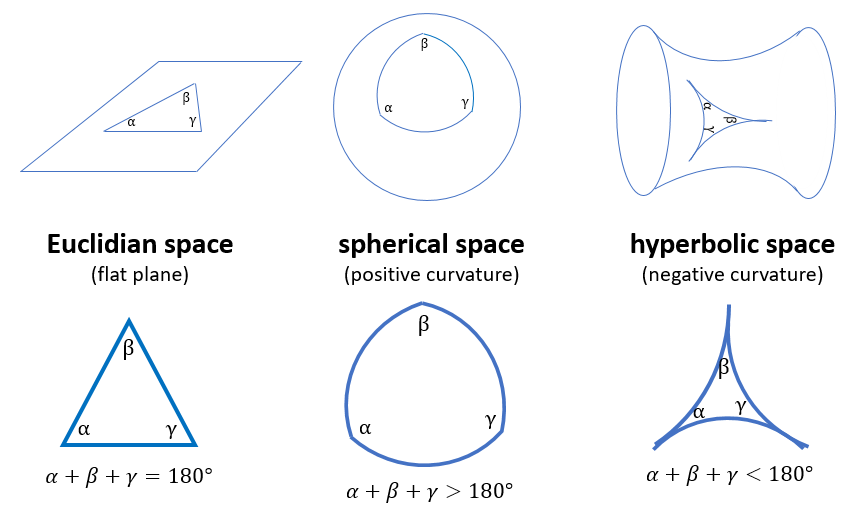
\includegraphics[width=0.67\linewidth]{Figures/non_euclidean.png}
    \caption{Representation of the three main types of geometry: Euclidean (flat), spherical (positive curvature), and hyperbolic (negative curvature). In each case, the sum of the angles of a triangle differs: it equals 180\textdegree{} in Euclidean geometry, exceeds 180\textdegree{} in spherical geometry, and is less than 180\textdegree{} in hyperbolic geometry. Source: \cite{Imatgenoneuclidean}.}
    \label{fig:noneuclidean}
\end{figure}



These ideas were once mathematical curiosities, but they became essential when Einstein formulated GR. In his theory, space-time is not flat but curved by the presence of mass and energy. The shortest paths, geodesics (see $\S$\ref{Geodesics and curvature}), no longer appear straight in the Euclidean sense but follow the curvature of space-time. This curved geometry, pioneered by \href{https://es.wikipedia.org/wiki/Bernhard_Riemann}{Bernhard Riemann}, provides the mathematical language to describe gravitational phenomena, replacing Newton’s force with the geometry of space-time itself.



\subsection{Manifolds and tangent spaces}
\label{Differentiable manifolds and coordinate systems}

In order to describe curved spaces mathematically, we use the concept of a manifold, which can be understood as a space that may possess curvature or a nontrivial topology, yet locally resembles Euclidean space. 

In more intuitive terms, an $N$-dimensional manifold $\mathcal{M}^N$ is a space that, in a neighborhood of each point $p \in \mathcal{M}^N$, looks like $\mathbb{R}^N$.  
At every point $p$ we can define the tangent space $T_p(\mathcal{M}^N)$, which is an $N$-dimensional vector space isomorphic\footnote{Two vector spaces \(\mathcal{A}\) and \(\mathcal{B}\) are considered isomorphic when there exists a bijective linear transformation \(f: \mathcal{A} \to \mathcal{B}\) whose inverse mapping \(f^{-1}: \mathcal{B} \to \mathcal{A}\) is also linear.
 In this case, \(\mathcal{A}\) and \(\mathcal{B}\) have the same algebraic structure and can be considered ``equivalent'' for all purposes of linear algebra.} to $\mathbb{R}^N$.  
Saying that a manifold is locally $\mathbb{R}^N$ means that, within a sufficiently small region around $p$, the tangent space $T_p(\mathcal{M}^N)$ provides an accurate linear approximation to the manifold.  
Nevertheless, tangent spaces at different points are distinct, reflecting the fact that the manifold is not globally flat (see Fig. \ref{fig:tangent space}).

\begin{figure}[h!]
    \centering
    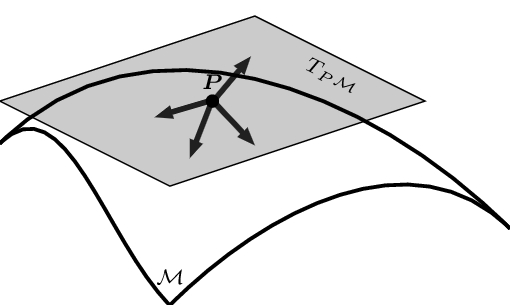
\includegraphics[width=0.5\linewidth]{Figures/Tangent_space_manifold.jpg}
    \caption{The set of all vectors defined at a point \(p\) forms the tangent space \(T_p(\mathcal{M})\) at \(p\). Assembling the tangent spaces for every point of the manifold produces the tangent bundle \(T(\mathcal{M})\).
 Original illustration based on the source: \cite{tangentspaceimage}.}
    \label{fig:tangent space}
\end{figure}

This intuitive picture is made precise by the definition of a topological manifold. 
Formally, an $N$-dimensional topological manifold is a topological space\footnote{A topological space consists of a set \(S\) together with a collection \(\mathcal{O}\) of its subsets, referred to as open sets, satisfying the following properties: (i) both \(S\) and the empty set are elements of \(\mathcal{O}\); (ii) any union, possibly infinite, of members of \(\mathcal{O}\) is also in \(\mathcal{O}\); and (iii) the intersection of finitely many members of \(\mathcal{O}\) belongs to \(\mathcal{O}\).  
The ordered pair \((S, \mathcal{O})\) is then called a topological space \cite{Coordinatebasis}.}
 $\mathcal{M}$ satisfying:
 
\begin{enumerate}
    \item Hausdorff property: for any two different points in \(\mathcal{M}\), there exist disjoint open sets, each containing one of the points.
    
    \item Second-countable: the topology on \(\mathcal{M}\) admits a basis consisting of a countable set.
    
    \item Locally Euclidean of dimension \(n\): every point \(p \in \mathcal{M}\) possesses an open neighborhood \(V \subset \mathcal{M}\) that is homeomorphic to an open subset of \(\mathbb{R}^n\).

\end{enumerate}

The last condition ensures that, although $\mathcal{M}$ may be globally curved, every point admits a ``patch'' that looks like a piece of flat $\mathbb{R}^n$. These patches provide the setting for introducing charts, which give local coordinates and allow us to describe the manifold in a precise mathematical language.

Manifolds appear throughout mathematics and physics. Examples include $\mathbb{R}^n$, spheres $S^n$, torus $T^n=S^1 \times \ldots \times S^1$, and Lie groups. In mechanics, the configuration space and phase space are manifolds; in thermodynamics, the state space defined by variables such as $(P,V,T)$ can be represented as a manifold. In GR, spacetime is modeled as a Lorentzian manifold (see $\S$\ref{metric tensor} for more details), which is locally isometric to Minkowski space but can have nontrivial global curvature determined by the distribution of matter and energy.

Thus, manifolds provide a rigorous framework for describing spaces that are locally simple but globally rich, equipped with smoothly overlapping coordinate systems, and with tangent structures that allow the precise definition of vectors, tensors, and other geometric objects essential in physics.


\subsubsection{Mappings, charts, and atlases}

A mapping between two sets represents the most fundamental concept in this framework. Given two sets \(\mathcal{M}\) and \(\mathcal{N}\), a map \(\phi: \mathcal{M} \to \mathcal{N}\) is a rule that associates to each element of \(\mathcal{M}\) precisely one element of \(\mathcal{N}\). Thus, a map can be viewed as a generalization of the traditional notion of a function.
 (see Fig. \ref{fig:mapping}). 

\begin{figure}[h!]
    \centering
    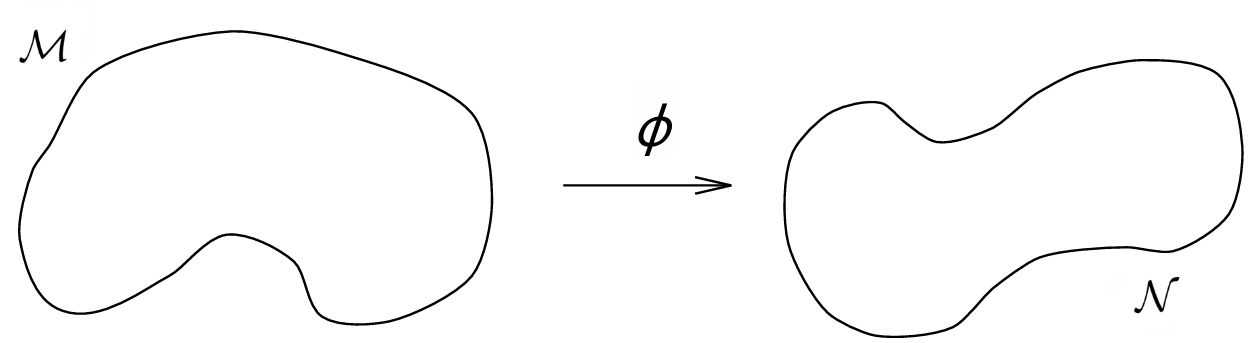
\includegraphics[width=0.56\linewidth]{Figures/mapping.png}
    \caption{Illustration of a mapping $\phi: \mathcal{M} \to \mathcal{N}$ between two sets, where each element of $\mathcal{M}$ is assigned precisely one element of $\mathcal{N}$. Source: \cite{llibrecarroll2004lectures}.}
    \label{fig:mapping}
\end{figure}

Given two mappings \(\varphi: A \to B\) and \(\psi: B \to C\), their composition \(\psi \circ \varphi: A \to C\) is defined by
\begin{equation}
(\psi \circ \varphi)(a) = \psi\bigl(\varphi(a)\bigr) \ ,
\end{equation}
where $\varphi$ acts first, followed by $\psi$.

In differential geometry, this concept is refined to describe the local structure of a manifold. A chart (also called a coordinate system) on a set \(\mathcal{M}\) is given by a subset \(U \subset \mathcal{M}\) along with an injective map \(\varphi: U \to \mathbb{R}^n\) such that the image \(\varphi(U) = \widetilde{U}\) forms an open subset of \(\mathbb{R}^n\).

Since any map is onto its image, the restricted map $\varphi: U \to \varphi(U)$ is invertible. In this setting, $U$ is regarded as an open subset of $\mathcal{M}$, and the components of
\begin{equation}
\varphi(p) = \bigl(x^1(p), \ldots, x^n(p)\bigr) \ ,
\end{equation}
are referred to as the local coordinates on \(U\).
If $\varphi(p) = 0$, the chart is said to be centered at the point $p$.

Intuitively, a chart can be thought of as a region of the manifold equipped with a coordinate system, much like a small patch of a curved surface represented on a flat map (see Fig. \ref{fig:chart}). 

\begin{figure}[h!]
    \centering
    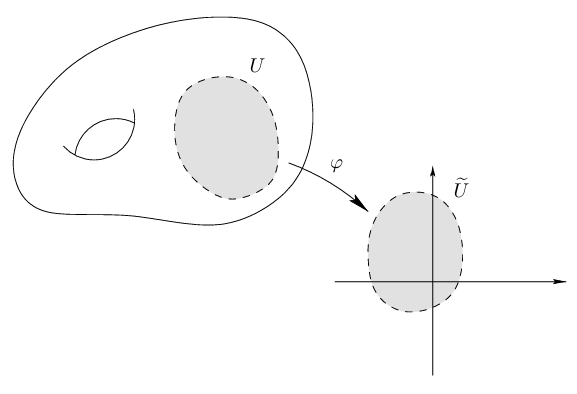
\includegraphics[width=0.55\linewidth]{Figures/Captura de pantalla 2025-08-01 183551.png}
    \caption{Representation of a chart $(U, \varphi)$ on a manifold $\mathcal{M}$, where the subset $U \subset \mathcal{M}$ is mapped bijectively to an open set $\widetilde{U} \subset \mathbb{R}^n$ via $\varphi$. This illustrates the local euclidean nature of manifolds. Source: \cite{Coordinatebasis}.}
    \label{fig:chart}
\end{figure}

However, just as it is impossible to represent the entire Earth on a single flat map without distortion (the classic ``cartographer's dilemma'' \cite{natgeo_cartographers_dilemma}), a single chart rarely covers the entire manifold. For example, $\mathbb{R}^n$ can be covered with a single chart, but the $2$-sphere $S^2$ cannot: a stereographic projection from the North Pole maps every point of $S^2$ except the North Pole itself to $\mathbb{R}^2$; conversely, projecting from the South Pole covers all but that point. Covering the whole $S^2$ requires at least two charts.

For this reason, we use a collection of charts. An atlas is a family of charts $\{(U_\alpha, \varphi_\alpha)\}$ whose domains cover $\mathcal{M}$ and satisfy two conditions:
\begin{enumerate}
    \item The collection of the domains covers the entire manifold:
    
    \begin{equation}
    \bigcup_\alpha U_\alpha = \mathcal{M} \ .
    \end{equation}
    \item The charts fit together smoothly: whenever $U_\alpha \cap U_\beta \neq \emptyset$, the transition map
    \begin{equation}
    \varphi_\beta \circ \varphi_\alpha^{-1}: \varphi_\alpha(U_\alpha \cap U_\beta) \to \varphi_\beta(U_\alpha \cap U_\beta) \ ,
    \end{equation}
    is a $C^\infty$ (smooth) function between open subsets of $\mathbb{R}^n$ (see Fig. \ref{fig:transition maps}).
\end{enumerate}


\begin{figure}[h!]
    \centering
    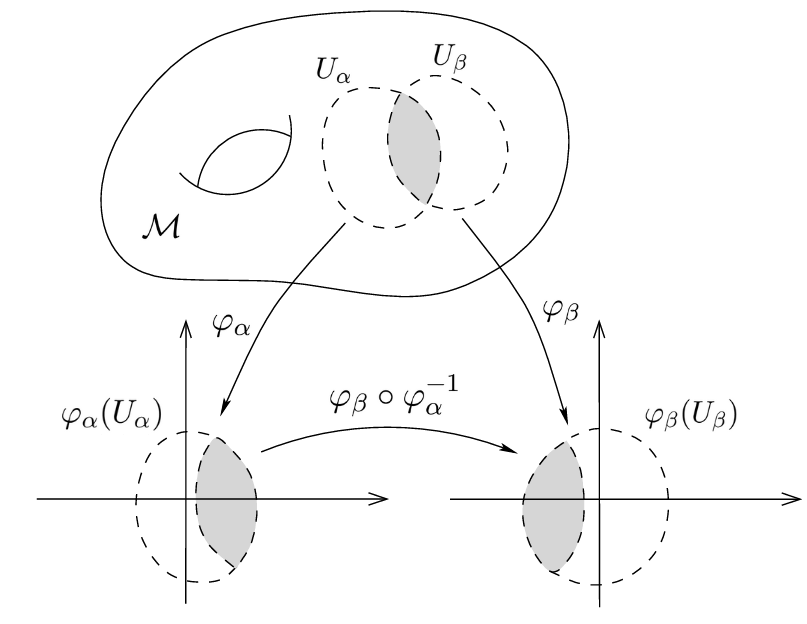
\includegraphics[width=0.58\linewidth]{Figures/transition maps.png}
    \caption{A chart is a patch $U$ of an $N$-dimensional manifold $M^N$ equipped with a mapping $\phi: U \to \mathbb{R}^N$ that defines a coordinate system on that region. When two charts overlap, their coordinate systems are related by a transformation that converts coordinates from one system to the other. Original illustration based on the source: \cite{Coordinatebasis}.}
    \label{fig:transition maps}
\end{figure}


These smooth transition maps ensure that the different ``local euclidean versions'' of the manifold are consistently and continuously glued together. A maximal atlas is one that contains all charts compatible with a given set, uniquely determining the manifold's differentiable structure.






\subsection{Mathematical interlude}

\subsubsection{Einstein summation convention and dummy indices}

As we delve deeper into the mathematics of vectors and tensors, we’ll notice that certain patterns appear repeatedly in equations. One such recurring structure involves expressions where an index appears more than once within the same term. For example, consider the following:
\begin{equation}
    \sum_\mu V^\mu U_\mu \ .
\end{equation}
In this expression, the index $\mu$ appears both as a superscript and a subscript. It is summed over, meaning it serves as a dummy index, a placeholder variable that takes on all possible values of that index. The specific letter used doesn’t matter; for instance:
\begin{equation}
    \sum_\nu V^\nu U_\nu \ ,
\end{equation}
represents exactly the same expression. The key characteristics of this type of sum are: 
\begin{itemize}
    \item The index appears exactly two times in a single term.
    \item It appears once as a superscript (contravariant) index and once as a subscript (covariant) index.
    \item It implies summation over all possible values of the repeated index.
\end{itemize}

Einstein’s clever idea, known as the Einstein summation convention, was to omit the summation symbol altogether when this pattern appears. According to this convention, whenever an index is repeated once upstairs and once downstairs in a term, a summation over that index is assumed. So instead of writing:
\begin{equation}
    \sum_\mu V^\mu U_\mu \ ,
\end{equation}
we can simply write:
\begin{equation}
    V^\mu U_\mu \ ,
\end{equation}
and the summation is understood.

This notational shortcut was first introduced by Einstein in his 1916 paper The Foundation of the General Theory of Relativity \cite{einstein1916foundation}. At the beginning of the paper, he still wrote out summation signs explicitly. For instance:
\begin{equation}
    dX_\nu = \sum_\sigma a_{\nu \sigma} \, dx_\sigma \ .
\end{equation}
However, shortly after equation 7, he casually notes that whenever an index appears twice, summation is to be assumed, and from then on, he stops writing summation symbols.

This convention is especially useful when working with vector and tensor algebra. For instance, we can represent the components of a column vector with upper indices, and those of a row vector with lower indices:
\begin{equation}
\begin{aligned}
    \vec{u} = u^i \quad \text{for} \quad i = 1, 2, 3, \dots, M \ , \\
    \vec{v} = v_j \quad \text{for} \quad j = 1, 2, 3, \dots, N \ .
\end{aligned}
\end{equation}
Here, $\vec{u}$ is a column vector of dimension $M \times 1$, and $\vec{v}$ is a row vector of dimension $1 \times N$. Their inner product, using Einstein notation, is:
\begin{equation}
    \vec{u} \cdot \vec{v} = u^i v_i \ ,
\end{equation}
which implies a summation over the index $i$.

We can also use this notation to construct matrices. For example, the outer (tensor) product of a column vector and a row vector is:
\begin{equation}
    \vec{A} = \vec{u} \otimes \vec{v} \ ,
\end{equation}
and in component form:
\begin{equation}
    A^i_{\ j} = u^i v_j = (u \otimes v)^i_{\ j} \ ,
\end{equation}
where the upper index $i$ denotes the row and the lower index $j$ the column.

The product of two matrices $A$ and $B$ to form a new matrix $C = AB$ becomes:
\begin{equation}
    C^i_{\ j} = A^i_{\ k} B^k_{\ j} \ .
\end{equation}
Here, the repeated index $k$ is summed over, while $i$ and $j$ remain free indices\footnote{Indices that appear once in a term are called free indices.}; they must appear identically on both sides of the equation. Note that we can change the order of multiplication:
\begin{equation}
    A^i_{\ k} B^k_{\ j} = B^k_{\ j} A^i_{\ k} \ ,
\end{equation}
but generally,
\begin{equation}
    A^i_{\ k} B^k_{\ j} \neq B^i_{\ k} A^k_{\ j} \ .
\end{equation}
The Einstein summation convention offers a powerful and elegant notational tool, widely used in physics and mathematics to simplify the representation of tensor equations \cite{LlibreBertJanssen, llibretheoreticalminimum}.


\subsubsection{Scalars, vectors and one-forms} 

In order to understand the formal structure and transformation properties of tensors in differential geometry and mathematical physics, it is essential to establish a foundational understanding of the objects from which tensors generalize: scalars, vectors, and one-forms. These entities constitute the building blocks of tensor calculus and each embodies a specific geometric and algebraic role in the representation of physical quantities and differential structures \cite{llibretensorcalculus}.
    
\paragraph{Scalars}


A scalar is defined as a quantity that is invariant under changes of coordinates. In physical and mathematical terms, this means that the value of a scalar remains the same regardless of the observer’s reference frame or the coordinate chart used.

Typical examples of scalar quantities include temperature, mass, and electric charge. These quantities are completely described by a single numerical value and do not depend on direction or orientation. Since scalars do not transform under coordinate changes, they serve as invariant reference points in both geometrical and physical analyses.

\paragraph{Vectors (contravariant)}

A vector is a geometric object characterized by both its magnitude and direction. In the context of differential geometry, vectors are identified as elements of the tangent space at a point on a differentiable manifold. When expressed in a local coordinate basis $\left\{ \frac{\partial}{\partial x^i} \right\}$\footnote{Given a local coordinate system $(x^1, \dots, x^n)$ on a manifold $\mathcal{M}$, 
the vectors $\frac{\partial}{\partial x^i}\big|_p$ represent the tangent directions at a point $p \in \mathcal{M}$. 
They form the natural basis of the tangent space $T_p\mathcal{M}$ corresponding to the chosen coordinates \cite{Coordinatebasis}.}, a vector $\vec{v}$ is written as:
\begin{equation}
\vec{v} = v^i \frac{\partial}{\partial x^i} \ .
\end{equation}
Here, the set $\{ v^i \}$ represents the components of the vector with respect to the given coordinate system. These components are said to be contravariant, since under a coordinate change \(x \mapsto x'\) they transform according to the Jacobian matrix of the transformation:
\begin{equation}
v'^{j} = \frac{\partial x'^j}{\partial x^i} v^i \ .
\end{equation}
This transformation law ensures that the geometric meaning of the vector, independent of coordinates, remains intact, while its components adjust to reflect the change in basis vectors. 

\paragraph{One-forms (covariant vectors)}

A one-form, also referred to as a covariant vector\footnote{The concepts of covariant and contravariant were first introduced by James Joseph Sylvester in 1851 \cite{Contravariant_covariant}.
} or linear form, is an element of the dual space\footnote{The dual space \(\mathcal{V}^*\) of a vector space \(\mathcal{V}\) is defined as the collection of all linear maps \(\ell: \mathcal{V} \to \mathbb{R}\) that assign a real number to each vector in \(\mathcal{V}\).  
For a manifold \(\mathcal{M}\), the tangent space \(T_p \mathcal{M}\) at a point \(p\) possesses a corresponding dual space, the cotangent space \(T_p^* \mathcal{M}\), whose elements are called covectors. One-forms are smooth assignments of a covector in \(T_p^* \mathcal{M}\) to each point \cite{Coordinatebasis}. } to the tangent space. Whereas vectors act as directional derivatives on scalar fields, one-forms act on vectors to produce scalars through a process of dual pairing. In coordinates, a one-form $\omega$ is written as:
\begin{equation}
\omega = \omega_i \, dx^i \ .
\end{equation}
Here, $\{ dx^i \}$ denotes the dual basis to $\left\{ \frac{\partial}{\partial x^i} \right\}$, and the components $\omega_i$ are said to be covariant. Their transformation under a coordinate change is governed by the inverse Jacobian:
\begin{equation}
\omega'_j = \frac{\partial x^i}{\partial x'^j} \omega_i \ .
\end{equation}

\subsubsection{Tensors}


The concept of a tensor is often cited as one of the most confusing topics for physics students. This confusion stems not from the intrinsic complexity of tensors, but rather from the overwhelming variety of definitions and the abstract formalism in which they are typically introduced. Many definitions focus not on what a tensor is, but on how it transforms under coordinate changes, which, though mathematically correct, offers little intuitive insight at first encounter.

At a fundamental level, a tensor can be seen as a generalization of familiar mathematical objects such as scalars and vectors.  
A scalar, which is a tensor of rank zero, is a single quantity invariant under coordinate transformations,  
whereas a vector, a rank-one tensor, has components that transform linearly with respect to these changes.


Tensors are commonly classified in two ways \cite{Llibre_Peter_Collier_unacosadificildecomprender}:

\begin{enumerate}
    \item By their rank or order, which corresponds to the total number of indices.  
    \item By their type $(n,m)$, where $n$ denotes the number of contravariant (upper) indices 
    and $m$ denotes the number of covariant (lower) indices.  
\end{enumerate}

Some illustrative examples are:

\begin{itemize}
    \item A scalar $T$ (e.g., temperature) carries no indices; it is a rank-$0$ tensor of type $(0,0)$.  
    \item A contravariant vector \(V^{\beta}\) carries a single upper index, making it a rank-one tensor of type \((1,0)\).  
    \item A covector or one-form $W_\alpha$ has one lower index, making it a rank-$1$ tensor of type $(0,1)$.  
    \item A mixed tensor \(T^\alpha_{\ \gamma}\) possesses one upper and one lower index, thus qualifying as a rank-two tensor of type \((1,1)\). 
    \item A purely contravariant tensor $S^{\beta\alpha}$ with two upper indices is rank $2$ and type $(2,0)$.  
    \item The Riemann curvature tensor $R^l{}_{ijk}$, which will be studied later, has one upper and three lower indices, making it a rank-$4$ tensor of type $(1,3)$.  
\end{itemize}

In general, a tensor of rank \(n\) in a $d$-dimensional space has $d^n$ components, each labeled by $n$ indices, 
and its components transform according to precise rules under coordinate changes.

These transformation rules are key. A rank-3 tensor of type (2, 1) transforms as:
\begin{equation}
T_\gamma^{\prime \alpha \beta}=\frac{\partial x^{\prime \alpha}}{\partial x^\mu} \frac{\partial x^{\prime \beta}}{\partial x^\nu} \frac{\partial x^\rho}{\partial x^{\prime \gamma}} T_\rho^{\mu \nu},
\end{equation}
where the prime symbol identifies the new coordinates and the transformed tensor.
 
More generally, a tensor of type $(r,s)$ transforms as:
\begin{equation}
T'^{i_1' \dots i_r'}_{j_1' \dots j_s'} = 
\left( \prod_{k=1}^r \frac{\partial x'^{i_k'}}{\partial x^{i_k}} \right)
\left( \prod_{l=1}^s \frac{\partial x^{j_l}}{\partial x'^{j_l'}} \right)
T^{i_1 \dots i_r}_{j_1 \dots j_s} \ .
\end{equation}
Such transformation behavior ensures that if a tensor equation holds in one coordinate system, it holds in all coordinate systems, an essential feature for any generally covariant physical theory, such as GR.


In practical terms, tensors enable us to express physical laws in a form that is independent of the observer’s frame of reference. For instance, if all components of a tensor vanish in one frame, they vanish in every frame. Similarly, if two tensors are equal in one coordinate system, they are equal in all. This coordinate-independence makes tensors the natural language for formulating physical laws that must remain valid regardless of how we choose to describe spacetime.

Tensors are not just abstract algebraic objects, they have clear geometric and physical interpretations. In mechanics, they describe stress and strain; in electrodynamics, they represent fields; and in GR, they encode curvature, energy, and momentum. 

Formally, a tensor of type $(r,s)$ can be seen as a multilinear map:
\begin{equation}
T: \underbrace{T^*_p \times \cdots \times T^*_p}_{k \text{ dual vectors}} \times \underbrace{T_p \times \cdots \times T_p}_{l \text{ vectors}} \rightarrow \mathbb{R} \ ,
\end{equation}
which takes $r$ covectors and $s$ vectors as inputs and returns a real number, 
linear in each argument \cite{Theory_of_Gravitational_Waves_arxiv}. 
In this view, upper indices correspond to ``slots'' for one-forms, 
and lower indices to ``slots'' for vectors. 
When all slots are filled, the tensor produces a scalar.


In a spacetime with no preferred coordinate system, as in GR, it is natural and necessary to express physical laws using tensor equations. These equations remain valid regardless of how we label spacetime points. In this context, tensors are not merely mathematical tools; they are the very grammar of the theory. 

Although their formal definitions can appear opaque, tensors are indispensable to modern physics. They allow us to write laws that are both general and coordinate-independent, making them essential for understanding and formulating the principles of reneral relativity.



\paragraph{Rules of tensor algebra}
\label{Rules of tensor algebra}

The basic algebraic operations familiar from vector spaces, such as scalar multiplication, addition, and the formation of inner and outer products, extend naturally to tensors of any rank, regardless of whether their indices are covariant or contravariant. These operations, which allow us to construct new tensors from existing ones, are often most clearly understood through illustrative examples \cite{llibretensorcalculus}.


\textbf{Scalar multiplication.} Multiplying a tensor by a scalar $a$ yields a new tensor of the same type
\begin{equation}
    T_{\mu \nu}=a S_{\mu \nu} \ .
\end{equation}
\textbf{Addition and subtraction.} Tensors of the same rank and index configuration can be added by summing their corresponding components to produce another tensor of the same type. Subtraction is simply addition with one tensor multiplied by a negative scalar
\begin{equation}
T^\mu{ }_\nu=S^\mu{ }_\nu+R^\mu{ }_\nu \ .
\end{equation}
\textbf{Multiplication.} The product of two tensors results in another tensor whose rank equals the sum of the ranks of the original tensors
\begin{equation}
T_\sigma^{\mu \nu \rho}=A_\sigma^\mu S^\nu R^\rho \ .
\end{equation}
\textbf{Contraction.} The rank of a tensor can be reduced by contraction, which pairs one contravariant and one covariant index and sums over it, mapping a $(r,s)$ tensor to a $(r-1,s-1)$ tensor
\begin{equation}
T_\nu=S_{\mu \nu} R^\mu \ .
\end{equation}
Contracting all indices of an even-order tensor yields a scalar\footnote{The proof is straightforward. Under a coordinate transformation,
\begin{equation}
R'^{\mu}{}_{\mu} = \frac{\partial x'^{\mu}}{\partial x^{\rho}} \frac{\partial x^{\nu}}{\partial x'^{\mu}} R^{\rho}{}_{\nu} 
= \delta^{\nu}_{\rho} R^{\rho}{}_{\nu} 
= R^{\rho}{}_{\rho},
\end{equation}
showing that the contraction produces an invariant quantity, namely a scalar \cite{llibretensorcalculus}.}. 
\begin{equation}
\begin{aligned}
R^{\mu}{}_{\mu} &= R  \ , \\
S^{\mu \nu}{}_{\mu \nu} &= S \ .
\end{aligned}
\end{equation}
\textbf{Raising and lowering indices.} A fundamental operation in tensor analysis is the contraction with the metric tensor $g_{\mu\nu}$ (see $\S$\ref{metric tensor} for more details) and its inverse $g^{\mu\nu}$ (sometimes referred to as the dual metric) to raise and lower indices in tensor expressions. This procedure allows us to convert vectors and covectors into one another by raising and lowering indices
\begin{equation}
\begin{aligned}
T_\nu &= g_{\mu\nu} T^\mu \ , \\
T^\nu &= g^{\mu\nu} T_\mu \ .
\end{aligned}
\end{equation}
Raising or lowering an index does not alter its relative position among the other indices. Furthermore, free indices (those not summed over) must match on both sides of an equation, while dummy indices (summed over) appear only once within each term.

\textbf{Symmetrization and antisymmetrization.} A tensor is symmetric in a set of indices if it remains unchanged when those indices are interchanged. For example, if
\begin{equation}
S_{\mu\nu\rho} = S_{\nu\mu\rho} \ ,
\end{equation}
it is symmetric in its first two indices. If it is invariant under all permutations of three indices, it is symmetric in all three. Examples of such tensors include the metric tensor and the Einstein tensor.

Similarly, a tensor is antisymmetric in certain indices if swapping them changes its sign; e.g.,
\begin{equation}
A_{\mu\nu\rho} = -A_{\rho\nu\mu} \ ,
\end{equation}
means antisymmetry in the first and third indices. The Riemann curvature tensor \( R^h_{\;ijk} \) (see $\S$\ref{Riemann curvature tensor} for more details) is antisymmetric in both its first and second index pairs:
\begin{equation}
R^h_{\;ijk} = -R^h_{\;jik} = -R^h_{\;ij\,k} \ .
\end{equation}
When a tensor exhibits symmetry or antisymmetry across all of its indices, it is referred to as symmetric or antisymmetric (sometimes described as fully symmetric or antisymmetric). The metric tensor \( g_{\mu\nu} \) and its inverse possess symmetry in their indices, whereas the Levi-Civita tensor \( \epsilon_{\mu\nu\rho\sigma} \) is characterized by antisymmetry.


Given any tensor, we can symmetrise or antisymmetrise over a chosen set of upper or lower indices.

Symmetrisation:
\begin{equation}
T_{(\mu_1 \mu_2 \dots \mu_p)} = \frac{1}{p!} \sum_{\text{perms}} T_{\mu_1 \mu_2 \dots \mu_p} \ .
\end{equation}
Antisymmetrisation:
\begin{equation}
T_{[\mu_1 \mu_2 \dots \mu_p]} = \frac{1}{p!} \sum_{\text{perms}} (\pm 1) \, T_{\mu_1 \mu_2 \dots \mu_p} \ ,
\end{equation}
where the sign \((\pm 1)\) depends on whether the permutation is even or odd.

Parentheses \((\dots)\) denote symmetrisation, and square brackets \([\dots]\) denote antisymmetrisation. To exclude certain indices, we use vertical bars:
\begin{equation}
T_{(\mu|\rho|\nu)} = \frac{1}{2} \left( T_{\mu\rho\nu} + T_{\nu\rho\mu} \right).
\end{equation}
Including the factor \( 1/p! \) ensures that repeated symmetrisation or antisymmetrisation of an already (anti)symmetric tensor has no effect.

For a rank-2 tensor \( T_{\mu\nu} \), the symmetric and antisymmetric parts are:
\begin{equation}
T_{\left(\mu\nu\right)} = \frac{1}{2} (T_{\mu\nu} + T_{\nu\mu}) \ , 
\quad
T_{[\mu\nu]} = \frac{1}{2} (T_{\mu\nu} - T_{\nu\mu}) \ .
\end{equation}
These definitions extend naturally to higher-rank tensors, even when the indices involved are not adjacent \cite{llibrecarroll2004lectures}.


\subsection{Metric tensor}
\label{metric tensor}

Until now, we have not introduced the most crucial element. There is a single object that, when defined on a manifold, surpasses all others in importance for understanding gravity: the metric tensor. The presence of a metric opens the door to a wide range of new concepts, which together form the framework known as Riemannian geometry \cite{llibretongGR}.

A differentiable manifold equipped with a symmetric metric tensor is called a Riemannian manifold. In GR, the metric plays a fundamental role: it defines the separation between nearby points in spacetime and determines the curvature of the manifold. In flat spacetime, far from matter and energy, the metric approximates the Minkowski metric $\eta_{\mu\nu}$ of special relativity \cite{llibreschutzGR}. Near massive objects, such as in the Schwarzschild solution, the metric adapts to reflect spacetime curvature (see $\S$\ref{Schwarzschild solution} for more details).

A metric tensor $g$ on a differentiable manifold $\mathcal{M}$ is a $(0,2)$ tensor field that allows the definition of an inner product on each tangent space $T_p(\mathcal{M})$. It satisfies:
\begin{itemize}
\item Symmetry: $g(X, Y) = g(Y, X)$ for all vector fields $X, Y$.
\item Non-degeneracy: If $g(X, Y)|_p = 0$ for all $Y \in T_p(M)$, then $X_p = 0$.
\end{itemize}
In a coordinate basis $\{ \partial_\mu \}$, the components of the metric are given by
\begin{equation}
g_{\mu\nu}(x) = g\left( \frac{\partial}{\partial x^\mu}, \frac{\partial}{\partial x^\nu} \right),
\end{equation}
and by definition
\begin{equation}
g_{\mu\nu} = e_\mu \cdot e_\nu \ ,
\end{equation}
where $e_\mu$ are the coordinate basis vectors.

Given coordinates $x^\mu$, an infinitesimal displacement in the manifold is
\begin{equation}
ds = dx^\mu\, e_\mu \ ,
\end{equation}
and its squared norm (inner product with itself) is
\begin{equation}
(ds)^2 = (dx^\mu e_\mu) \cdot (dx^\nu e_\nu) \overset{(i)}{=} g_{\mu\nu}\, dx^\mu dx^\nu.
\end{equation}
\noindent\hspace{1cm} $(i)$ We use that $e_\mu \cdot e_\nu = g_{\mu\nu}$.

This is the line element:
\begin{equation}
ds^2 = g_{\mu\nu}(x)\, dx^\mu dx^\nu.
\end{equation}
In an $n$-dimensional Riemannian manifold:
\begin{equation}
dl^2 = g_{ij}\, dx^i dx^j \ .
\end{equation}
Similarly, the inner product of two distinct vectors is
\begin{equation}
V \cdot W = g_{\mu\nu} V^\mu W^\nu \ .
\end{equation}
The explicit form of $g_{\mu\nu}$ depends on the coordinate system \cite{llibretensorcalculus}. In Cartesian coordinates:
\begin{equation}
dl^2 = dx^2 + dy^2 + dz^2, \quad g_{ij} =
\begin{pmatrix}
1 & 0 & 0 \\
0 & 1 & 0 \\
0 & 0 & 1
\end{pmatrix}.
\end{equation}
In Minkowski spacetime:
\begin{equation}
ds^2 = c^2 dt^2 - dx^2 - dy^2 - dz^2, \quad \eta_{\mu\nu} =
\begin{pmatrix}
1 & 0 & 0 & 0 \\
0 & -1 & 0 & 0 \\
0 & 0 & -1 & 0 \\
0 & 0 & 0 & -1
\end{pmatrix}.
\end{equation}
In spherical coordinates:
\begin{equation}
ds^2 = dr^2 + r^2\, d\theta^2 + r^2 \sin^2\theta\, d\varphi^2, \quad g_{ij} = \mathrm{diag}(1, r^2, r^2\sin^2\theta)\footnote{The notation \(\mathrm{diag}(a_1, a_2, \dots, a_n)\) denotes a diagonal matrix whose entries are zero everywhere except along the diagonal, where the components are \(a_1, a_2, \dots, a_n\). In this case, it means that the metric tensor \(g_{ij}\) has components \(g_{11} = 1\), \(g_{22} = r^2\), \(g_{33} = r^2\sin^2\theta\), and all off-diagonal components vanish \cite{llibrehassani2009}.}.
\end{equation}
In general, $g_{\mu\nu}$ is a symmetric $4 \times 4$ matrix in spacetime, with $10$ independent components. Because coordinate transformations can adjust 4 of them, only $6$ components contain independent physical information \cite{Llibrehartle2003gravity}.

The metric tensor is the tool that enables the computation of lengths, angles, areas, and volumes in a manifold. In physics, it encodes the gravitational field in GR. It also acts as a bridge between contravariant and covariant vectors (as we have seen in $\S$\ref{Rules of tensor algebra}):
\begin{equation}
v_\mu = g_{\mu\nu} v^\nu, \quad v^\mu = g^{\mu\nu} v_\nu \ ,
\end{equation}
where $g^{\mu\nu}$ is the inverse metric, satisfying
\begin{equation}
g_{\mu\nu} g^{\nu\rho} = \delta_\mu^\rho \ .
\end{equation}
The signature of the metric distinguishes between different geometries: Riemannian metrics are positive-definite $(+,+,+,\dots)$, while Lorentzian metrics have signature $(+,-,-,\dots,-)$ or $(-,+,+,\dots,+)$ as in spacetime. Once the metric is known, the geometry and the gravitational field (in the case of GR) are completely determined.



\subsection{Affine connection and curvature}

We’ve now laid the groundwork for a deeper look into the mathematics of curved space. Ultimately, our goal is to understand:

\begin{itemize}
    \item Geodesics (see $\S$\ref{Geodesics and curvature}), the “straightest possible” paths between any two points on a Riemannian manifold, and thus the natural trajectories of free particles moving through curved spacetime.  
    \item The Riemann curvature tensor (see $\S$\ref{Riemann curvature tensor}), which encodes how space bends. A particular version of this tensor appears on the left-hand side of the fundamental object of GR, the Einstein field equations (EFE).
\end{itemize}

Parallel transport of a vector (see $\S$\ref{parallel transport}) plays a key role in both of these concepts. But before we can understand how to transport vectors, we must first know how to differentiate tensor fields. To make this possible, we introduce what are known as connection coefficients or Christoffel symbols (denoted by the symbol $\Gamma$). These coefficients allow us to compare vectors located at different points on a manifold. Once the metric of the manifold is known, we can compute the connection coefficients, unlocking our ability to define derivatives and do much more. This is why the metric is central to understanding Riemannian manifolds, and therefore the geometry of spacetime itself \cite{Llibre_Peter_Collier_unacosadificildecomprender}.


\subsubsection{Christoffel symbols}

Our goal in GR is to express physical laws as tensor equations valid in any coordinate system. To do that, we must be able to differentiate tensors in a way that behaves well under changes of coordinates. Specifically, we want a derivative that reduces to the usual partial derivative in flat Minkowski space using Cartesian coordinates, but which still transforms as a tensor in curved spacetimes.

At first glance, differentiating a tensor might seem straightforward. For example, in Cartesian coordinates, a vector field like
\begin{equation}
\vec{V}(x, y, z) = (2x - y)\, \vec{e}_x + (x + 3z)\, \vec{e}_y + (y - z)\, \vec{e}_z \ ,
\end{equation}
can be differentiated component by component: 
\begin{equation}
\frac{\partial \vec{V}}{\partial x} = 2\, \vec{e}_x + \vec{e}_y \ , \quad \quad 
\frac{\partial \vec{V}}{\partial y} = -\, \vec{e}_x + \vec{e}_z \ , \quad \quad
\frac{\partial \vec{V}}{\partial z} = 3\, \vec{e}_y - \vec{e}_z \ .
\end{equation}
The basis vectors $\vec{e}_x, \vec{e}_y, \vec{e}_z$ are constant in space, so we don’t need to worry about them changing from point to point. We just apply the partial derivative to each component function.

However, this approach fails in curved spaces or curvilinear coordinates, where the basis vectors themselves vary from point to point. In such cases, when differentiating a tensor, we must also account for the rate of change of the basis vectors. This is where the connection coefficients, or Christoffel symbols, come into play.

Let us consider a vector expressed as $\vec{V} = V^\alpha \vec{e}_\alpha$, where $\vec{e}_\alpha$ are the coordinate basis vectors. Now let’s take the derivative of this with respect to some coordinate using the product rule \cite{Llibre_Peter_Collier_unacosadificildecomprender}:
\begin{equation}
    \frac{\partial \vec{V}}{\partial x^\beta} 
= \frac{\partial}{\partial x^\beta} \left( V^\alpha \vec{e}_\alpha \right) 
= \left( \frac{\partial V^\alpha}{\partial x^\beta} \right) \vec{e}_\alpha 
+ V^\alpha \left( \frac{\partial \vec{e}_\alpha}{\partial x^\beta} \right) \ .
\label{vectorderivative}
\end{equation}
The first term reflects the change in the vector components, while the second term captures how the basis vectors change. Since $\partial_\beta \vec{e}_\alpha$ is itself a vector, it can be expressed in terms of the basis:
\begin{equation}
\frac{\partial \vec{e}_\alpha}{\partial x^\beta} = \Gamma^\gamma_{\alpha\beta} \vec{e}_\gamma \ .
\label{christoffelsymbols}
\end{equation}
Here, the Christoffel symbols $\Gamma^\gamma_{\alpha\beta}$ quantify how the basis vector $\vec{e}_\alpha$ changes in the direction of coordinate $x^\beta$, projected onto the basis $\vec{e}_\gamma$. The lower indices $\alpha$ and $\beta$ refer to the direction and variable of differentiation, while the upper index $\gamma$ indicates the output basis direction.


We can isolate the Christoffel symbol by multiplying both sides by the dual basis vector $\vec{\hspace{0.15em}e}^\gamma$:
\begin{equation}
\vec{\hspace{0.15em}e}^\gamma \cdot \partial_\beta \vec{e}_\alpha 
= \Gamma^\gamma_{\alpha \beta} \vec{\hspace{0.15em}e}^\gamma \cdot \vec{e}_\gamma 
\quad \Rightarrow \quad 
\Gamma^\gamma_{\alpha \beta} = \vec{\hspace{0.15em}e}^\gamma \cdot \partial_\beta \vec{e}_\alpha \ .
\end{equation}
Here, we used the property $\vec{\hspace{0.15em}e}^\beta \cdot \vec{e}_\alpha = \delta^\beta_\alpha$, which defines the dual basis and implies that $\vec{\hspace{0.15em}e}^\gamma \cdot \vec{e}_\gamma = 1$.


These coefficients do not form a tensor themselves, but they are essential for constructing tensorial derivatives.

Some key properties of Christoffel symbols are:
\begin{itemize}
    \item They provide the rule for differentiating tensors in a curved manifold.
    \item They are called connection coefficients because they ``connect'' nearby points on the manifold, defining how vectors vary between them, crucial for defining parallel transport.
    \item If we know the metric $g_{\mu\nu}$, we can compute them explicitly as (see Appendix $\S$\ref{Proofs and derivations} for the derivation):
    \begin{equation}
    \Gamma^\rho_{\mu\nu} = \frac{1}{2} g^{\rho\lambda} \left( \partial_\mu g_{\lambda\nu} + \partial_\nu g_{\lambda\mu} - \partial_\lambda g_{\mu\nu} \right) \ .
    \end{equation}
    \item In standard GR (without torsion\footnote{Torsion describes the amount of “asymmetry” in the way points in spacetime are connected: it indicates whether moving first in one direction and then in another ends at the same point as doing so in the reverse order. If torsion is zero, as in standard GR, both paths lead to the same point. When we study parallel transport and the Riemann curvature tensor (see $\S$\ref{Riemann curvature tensor}), this idea will acquire a precise mathematical formulation through the torsion tensor. See \cite{LlibreBertJanssen, torsion} for more details.}), the Christoffel symbols are symmetric in their lower indices:
    \begin{equation}
        \Gamma^\rho_{\mu\nu} = \Gamma^\rho_{\nu\mu} \ .
    \end{equation}
    \item In an $n$-dimensional Riemannian manifold, there are theoretically $n^3$ such coefficients, though this number is reduced by the symmetry condition.
\end{itemize}

The term ``Christoffel symbols'' honors the mathematician Elwin Christoffel (1829--1900), who first introduced them in the context of differential geometry. Although sometimes informally dubbed ``Christ-awful symbols'' due to their apparent complexity, this perception tends to fade with familiarity \cite{llibretheoreticalminimum}. What initially seems intricate is, in fact, a systematic way of incorporating the effects of curvature into the formulation of differential operators . 

These connection coefficients are essential for extending the familiar notion of differentiation to the curved spacetimes of GR, setting the stage for the definition of the covariant derivative, which we address next.



\subsubsection{Covariant derivative}


Having introduced the Christoffel symbols \eqref{christoffelsymbols} and established how to differentiate vectors in curved spacetime using equation \eqref{vectorderivative}, we are now ready to define the covariant derivative, which provides a consistent framework for differentiating tensors.


Substituting equation \eqref{christoffelsymbols} into equation \eqref{vectorderivative}, we obtain:
\begin{equation}
    \frac{\partial \vec{V}}{\partial x^\beta} 
=  \frac{\partial V^\alpha}{\partial x^\beta} \vec{e}_\alpha 
+ V^\alpha \Gamma^\gamma_{\alpha\beta} \vec{e}_\gamma \ .
\end{equation}
We relabel the dummy indices \(\alpha\) and \(\gamma\) in the right-hand side term, as they are summation indices and can be freely exchanged to simplify the expression:
\begin{equation}
    \frac{\partial \vec{V}}{\partial x^\beta} 
=  \frac{\partial V^\alpha}{\partial x^\beta} \vec{e}_\alpha 
+ V^\gamma \Gamma^\alpha_{\gamma\beta} \vec{e}_\alpha \ .
\end{equation}
We now factor out the common basis vector \(\vec{e}_\alpha\):
\begin{equation}
    \frac{\partial \vec{V}}{\partial x^\beta} 
=  \left(\frac{\partial V^\alpha}{\partial x^\beta}
+ V^\gamma \Gamma^\alpha_{\gamma\beta}\right) \vec{e}_\alpha \ .
\end{equation}
We can express the components of $\dfrac{\partial \vec{V}}{\partial x^\beta}$ as:
\begin{equation}
\frac{\partial V^\alpha}{\partial x^\beta} + V^\gamma \Gamma^\alpha_{\gamma \beta} \ .
\label{covariantderivative}
\end{equation}
This formula represents the covariant derivative of the contravariant vector $\vec{V}$. It describes how the component $V^\alpha$ changes in the direction $\beta$ of the coordinate system $x_\beta$. It is common to use the notation $\nabla_\beta V^\alpha$ to denote the covariant derivative, so equation \eqref{covariantderivative} can also be written as:
\begin{equation}
\nabla_\beta V^\alpha = \frac{\partial V^\alpha}{\partial x^\beta} + V^\gamma \Gamma^\alpha_{\gamma \beta} \ .
\end{equation}
Similarly, the covariant derivative of a one-form or covector is expressed as:
\begin{equation}
\nabla_\beta V_\alpha = \frac{\partial V_\alpha}{\partial x^\beta} - V_\gamma \Gamma^\gamma_{\alpha \beta} \ .
\end{equation}
The covariant derivative maintains the properties of linearity and satisfies the product rule, similar to the partial derivative:
\begin{equation}
\begin{aligned}
& \nabla_\mu (\alpha V^\nu + \beta W^\nu) = \alpha \nabla_\mu V^\nu + \beta \nabla_\mu W^\nu, \\
&\nabla_\mu (V^\nu W^\rho) = (\nabla_\mu V^\nu) W^\rho + V^\nu (\nabla_\mu W^\rho) \ .
\end{aligned}
\end{equation}
Moreover, it has the important property of transforming properly as a \((1,1)\) tensor:
\begin{equation}
\nabla_\alpha V^\gamma = \frac{\partial x^\mu}{\partial y^\alpha}\frac{\partial y^\gamma}{\partial x^\nu}\nabla_\mu V^\nu \ .
\end{equation}
Furthermore, in flat space and when working with Cartesian coordinates, the covariant derivative of a vector or a one-form simplifies to the partial derivative:
\begin{equation}
    \nabla_\alpha \phi = \partial_\alpha \phi \ .
\end{equation}
Finally we can see how to construct the covariant derivative of a tensor.


We derive the covariant derivative of a tensor of type $(1,1)$, that is, a tensor with one upper (contravariant) index and one lower (covariant) index. Our goal is to construct a derivative operator that preserves the tensorial nature of the object under coordinate transformations.

Let $T^\nu{}_\mu$ be a $(1,1)$ tensor. The covariant derivative $\nabla_\rho T^\nu{}_\mu$ is given by:
\begin{equation}
\nabla_\rho T^\nu{}_\mu = \partial_\rho T^\nu{}_\mu 
- \Gamma^\lambda_{\rho\mu} T^\nu{}_\lambda 
+ \Gamma^\nu_{\rho\lambda} T^\lambda{}_\mu \ .
\end{equation}
This formula can be understood as follows:

\begin{itemize}
    \item The first term $\partial_\rho T^\nu{}_\mu$ is the ordinary partial derivative.
    \item The second term $- \Gamma^\lambda_{\rho\mu} T^\nu{}_\lambda$ corrects for the transformation of the covariant index $\mu$.
    \item The third term $+ \Gamma^\nu_{\rho\lambda} T^\lambda{}_\mu$ corrects for the transformation of the contravariant index $\nu$.
\end{itemize}

The general rule is: for each lower index, subtract a term involving a Christoffel symbol; for each upper index, add a term involving a Christoffel symbol. This ensures that the resulting expression transforms properly as a tensor.

In general, the covariant derivative of a tensor of type $(m, n)$ is given by \cite{Llibre_Peter_Collier_unacosadificildecomprender}:
\begin{equation}
\begin{aligned}
\nabla_\rho T^{\mu_1 \dots \mu_m}_{\ \ \ \ \ \nu_1 \dots \nu_n} &= \partial_\rho T^{\mu_1 \dots \mu_m}_{\ \ \ \ \ \nu_1 \dots \nu_n}\\
&+ \Gamma^{\mu_1}_{\rho \lambda} T^{\lambda \mu_2 \dots \mu_m}_{\ \ \ \ \ \nu_1 \dots \nu_n}
+ \dots + \Gamma^{\mu_m}_{\rho \lambda} T^{\mu_1 \dots \mu_{m-1} \lambda}_{\ \ \ \ \ \nu_1 \dots \nu_n}\\
&- \Gamma^{\lambda}_{\rho \nu_1} T^{\mu_1 \dots \mu_m}_{\ \ \ \ \ \lambda \nu_2 \dots \nu_n}
- \dots
- \Gamma^{\lambda}_{\rho \nu_n} T^{\mu_1 \dots \mu_m}_{\ \ \ \ \ \nu_1 \dots \nu_{n-1} \lambda} \ .
\end{aligned}
\end{equation}
To ensure the internal consistency of GR, it is postulated that the covariant derivative of the metric tensor vanishes:
\begin{equation}
\nabla_\beta g_{\mu \nu} = \nabla_\beta g^{\mu \nu} = 0 \ .
\end{equation}
A covariant derivative satisfying this condition is referred to as metric compatible. This requirement ensures that the scalar product between vectors remains constant during parallel transport (see $\S$\ref{parallel transport}) across a curved spacetime manifold. While this condition holds trivially in flat spacetime (as in special relativity), it becomes a non-trivial and essential constraint in the presence of curvature.

Because the equation above is tensorial, it holds in all coordinate systems. More precisely, metric compatibility ensures that the inner product structure imposed by the metric remains invariant along curves. This allows meaningful operations such as raising and lowering indices and defining lengths and angles between vectors in curved geometry.

Although one can mathematically define connections for which $\nabla_\beta g_{\mu \nu} \neq 0$, such connections are not compatible with the metric and are generally not useful in the context of GR \cite{Llibre_Peter_Collier_unacosadificildecomprender}.


\subsubsection{Parallel transport }
\label{parallel transport}


To understand the geometry of curved spaces, one must move beyond the familiar tools of Euclidean geometry. In flat space, vectors at different points can be naturally compared, added, subtracted, or evaluated using inner products because transporting a vector from one point to another without changing its direction is unambiguous. However, this intuition breaks down in curved manifolds, where the concept of direction is local and the comparison of vectors at different points becomes nontrivial.

This leads to a fundamental question: how can we define the idea of keeping a vector “unchanged” as we move it along a path in a curved space? The answer lies in the notion of parallel transport. Parallel transport provides a rule for moving vectors along curves in a manifold in such a way that they remain as “constant” as possible according to the geometry of the space.

In flat space, transporting a vector around a closed loop brings it back unchanged. But in curved spaces, the result of parallel transport around a loop generally depends on the path taken, reflecting the intrinsic curvature of the manifold (see Fig. \ref{fig:paraleltransportflat}). 

\begin{figure}[h!]
    \centering
    \begin{subfigure}[t]{0.42\linewidth}
        \centering
        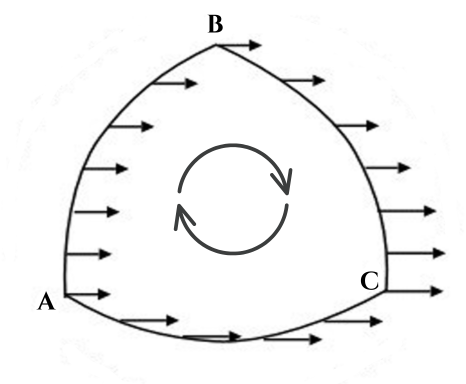
\includegraphics[width=\linewidth]{Figures/paralel transport flat.png}
        \caption{Parallel transport in flat space.}
    \end{subfigure}
    \hspace{0.5cm}
    \begin{subfigure}[t]{0.36\linewidth}
        \centering
        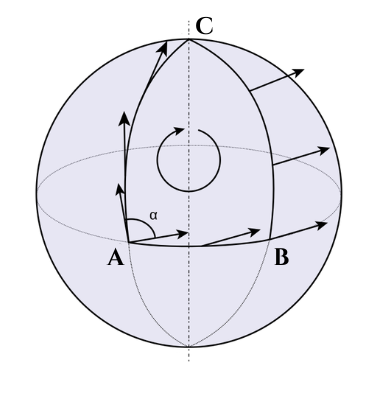
\includegraphics[width=\linewidth]{Figures/paralel transport curved.png}
        \caption{Parallel transport on a curved space (sphere).}
    \end{subfigure}
    \caption{Comparison between parallel transport in flat and curved spaces. In flat space, the vector returns unchanged after a closed loop; in curved space, the final result depends on the path taken, revealing the manifold's intrinsic geometry. Original illustrations based on the sources: \cite{Llibre_Peter_Collier_unacosadificildecomprender, ParallelTransportSvg}.}
    \label{fig:paraleltransportflat}
\end{figure}


The condition for the parallel transport of the vector $\vec{V}$ along a parametrized curve is that its covariant derivative with respect to the curve's parameter must be zero, namely,
\begin{equation}
    \frac{d\vec{V}}{d\lambda} = 0 \ .
\end{equation}
To obtain the derivative, we use equation \eqref{vectorderivative} and replace the parameter $x^{\beta}$ with $\lambda$, obtaining:
\begin{equation}
    \frac{d\vec{V}}{d\lambda} = \frac{dV^\alpha}{d\lambda} e_\alpha + V^\alpha \frac{d e_\alpha}{d\lambda} \ .
\end{equation}
The change of the basis can be expressed as
\begin{equation}
\frac{d e_\alpha}{d\lambda}
= \frac{\partial e_\alpha}{\partial x^\beta}\,\frac{dx^\beta}{d\lambda}
= \Gamma^\gamma_{\alpha\beta}\,\frac{dx^\beta}{d\lambda}\,e_\gamma \ ,
\end{equation}
were we have used the definition of the Christoffel symbols \eqref{christoffelsymbols}.


Substituting this result into the previous expression and replacing the index $\alpha$ with $\gamma$ in the first term yields
\begin{equation}
\frac{d\vec{V}}{d\lambda}
= \left(\frac{dV^\gamma}{d\lambda} + V^\alpha\,\Gamma^\gamma_{\alpha\beta}\,\frac{dx^\beta}{d\lambda}\right) e_\gamma \ .
\end{equation}
We define the absolute derivative\footnote{An absolute derivative refers to the covariant derivative taken along a curve, in this case the curve parametrized by $\lambda$.
} along the curve as
\begin{equation}
\frac{D V^\gamma}{d\lambda} \equiv \frac{dV^\gamma}{d\lambda} + \Gamma^\gamma_{\alpha\beta}\,V^\alpha\,\frac{dx^\beta}{d\lambda} \ ,
\end{equation}
or equivalently,
\begin{equation}
\frac{D}{d\lambda} \vec{V} = \frac{dx^\mu}{d\lambda}\,\nabla_\mu \vec{V}.
\end{equation}
Parallel transport of $\vec{V}$ along the curve is then defined by the condition
\begin{equation}
\frac{D\vec{V}}{d\lambda} = 0
\quad\Longleftrightarrow\quad
\frac{dV^\gamma}{d\lambda} + \Gamma^\gamma_{\alpha\beta}\,V^\alpha\,\frac{dx^\beta}{d\lambda} = 0 \ .
\end{equation}
This is a linear first order system of ordinary differential equations for the components $V^\gamma(\lambda)$, which, given initial data $V^\gamma(\lambda_0)$, has a unique solution along the curve.

For a tensor $T^{\mu_1\ldots\mu_p}{}_{\nu_1\ldots\nu_q}$ the parallel transport along a trajectory $x^\mu(\lambda)$ is defined by requiring that, for every point on the curve,

\begin{equation}
\left( \frac{D}{d\lambda} T \right)^{\mu_1\mu_2\ldots\mu_p}{}_{\nu_1\nu_2\ldots\nu_q}
\; \equiv \; \frac{dx^\sigma}{d\lambda} \, \nabla_\sigma T^{\mu_1\mu_2\ldots\mu_p}{}_{\nu_1\nu_2\ldots\nu_q} \; \equiv \; 0 \ .
\end{equation}

This expression constitutes a valid tensor equation because both the tangent vector $dx^\mu/d\lambda$ and the covariant derivative $\nabla_\mu$ transform as tensors. 
    
This equation plays a key role, as we will see in the next section that it serves as the starting point for deriving the geodesic equations. We will also find that freely moving or freely falling objects in spacetime follow the straightest possible paths, curves known as geodesics.


\subsubsection{Geodesics}
\label{Geodesics and curvature}


In Euclidean space, the shortest path between two points is a straight line. In a curved space, the analogous concept is a geodesic, a curve that, given the curvature of the space, is as ``straight'' as possible. On a sphere, for example, great circles play this role. 

The idea of a geodesic can be formalized in several equivalent ways when considering two points $A$ and $B$ on a surface \cite{llibretheoreticalminimum}:
\begin{enumerate}
    \item The geodesic is the curve that minimizes the distance between $A$ and $B$.
    \item A geodesic is a curve whose length remains stationary under small variations of its shape.
    \item A more local definition states that a geodesic is a curve that, at each point, is as straight as possible.
\end{enumerate}
There are also several equivalent ways to derive geodesics, each providing complementary insights.

\paragraph{Geometric derivation}

From a geometric perspective, a geodesic is defined as a curve whose tangent vector is parallel transported along itself. Formally, this condition requires that the covariant derivative of the tangent vector vanishes at every point of the curve \cite{LlibreBertJanssen}.  

Let \(x^\mu(\lambda)\) represent a parametrized curve, where \(\lambda\) is an affine parameter. Its tangent vector is given by
\begin{equation}
    U^\mu = \frac{dx^\mu}{d\lambda} \ .
\end{equation}
The requirement of parallel transport along the curve is expressed as
\begin{equation}
    \frac{D U^\mu}{d\lambda} = 0 \ ,
\end{equation}
which, using the explicit form of the covariant derivative, becomes
\begin{equation}
    \frac{dU^\mu}{d\lambda} + \Gamma^{\mu}_{\rho\sigma} \, U^\rho \frac{dx^\sigma}{d\lambda} = 0 \ .
\end{equation}
Substituting \(U^\rho = \frac{dx^\rho}{d\lambda}\), one arrives at the standard geodesic equation \cite{llibrecarroll2004lectures}:
\begin{equation}
    \frac{d^2 x^\mu}{d\lambda^2} + \Gamma^{\mu}_{\rho\sigma} \frac{dx^\rho}{d\lambda} \frac{dx^\sigma}{d\lambda} = 0 \ .
    \label{geodesicequation}
\end{equation}

Thus, the geodesic equation emerges naturally as the geometric condition ensuring that the tangent vector remains invariant under parallel transport.


\paragraph{Coordinate form and free fall}


Complementarily, the same equation can be derived from a physical perspective, starting from the principle of inertia in a locally inertial frame.

In such a frame, for example, that of a freely falling observer, the Christoffel symbols vanish, and the motion of a freely falling particle is described simply by 
\begin{equation}
    \frac{d^2 X^\alpha}{d\tau^2} = 0 \ ,
    \label{eq:freefalllocal}
\end{equation}
where $\tau$ denotes the particle's proper time and $X^\alpha$ are coordinates in the local inertial frame \cite{llibretensorcalculus}.  

We now relate the locally inertial coordinates $X^\alpha$ to a general coordinate system $x^\mu$ through a transformation
\begin{equation}
    X^\alpha = X^\alpha(x^\mu(\tau)) \ .
\end{equation}
Since $X^\alpha$ depends on all $x^\mu$, differentiating equation \eqref{eq:freefalllocal} and applying the chain rule gives
\begin{equation}
    \frac{\partial X^\alpha}{\partial x^\mu} \frac{d^2 x^\mu}{d\tau^2} 
    + \frac{\partial^2 X^\alpha}{\partial x^\mu \partial x^\nu} 
      \frac{dx^\mu}{d\tau} \frac{dx^\nu}{d\tau} = 0 \ ,
\end{equation}

where we have used $\frac{d}{d\tau}
= \frac{dx^\nu}{d\tau}\,\frac{\partial}{\partial x^\nu}$ for the second term.

Multiplying by $\frac{\partial x^\lambda}{\partial X^\alpha}$ and using
\begin{equation}
    \frac{\partial x^\lambda}{\partial X^\alpha} \frac{\partial X^\alpha}{\partial x^\mu} 
    = \delta^\lambda_\mu \ ,
\end{equation}
we obtain
\begin{equation}
    \frac{d^2 x^\lambda}{d\tau^2} 
    + \Gamma^{\lambda}_{\mu\nu} \frac{dx^\mu}{d\tau} \frac{dx^\nu}{d\tau} = 0 \ ,
    \label{newtons2nlaw}
\end{equation}
where the connection coefficients appear naturally as
\begin{equation}
    \Gamma^{\lambda}_{\mu\nu} 
    = \frac{\partial x^\lambda}{\partial X^\alpha} 
      \frac{\partial^2 X^\alpha}{\partial x^\mu \partial x^\nu} \ .
\end{equation}
The main physical significance of geodesics in GR lies in the fact that they describe the trajectories of freely falling particles, objects experiencing no proper acceleration. Within this framework, the geodesic equation serves as the relativistic analogue of Newton's second law, \(\vec{F} = m \vec{a}\), specifically in the case where \(\vec{F} = 0\).


\paragraph{Action principle and lagrangian formulation}

Geodesics can also be derived from a variational principle. We consider the relativistic action of a particle traveling through spacetime, given by
\begin{equation}
S = -m \int_{\tau_1}^{\tau_2} \mathcal{L} \, d\tau \ , \quad \text{where} \quad \mathcal{L} = \sqrt{-g_{\mu\nu}(x) \dot{x}^\mu \dot{x}^\nu} \ ,
\end{equation}
with \( m \) representing the particle's mass and \( \dot{x}^\mu=dx^{\mu}/d\tau \).

Applying the Euler-Lagrange equations to this Lagrangian, 
the stationarity condition $\delta S = 0$ yields
\begin{equation}
    \frac{d}{d\tau}\left(\frac{\partial L}{\partial \dot{x}^\lambda}\right) 
    - \frac{\partial L}{\partial x^\lambda} = 0 \ .
    \label{eulerlagrange}
\end{equation}
We define the quantity
\begin{equation}
I(x,\dot{x}) \equiv - g_{\mu\nu}(x)\, \dot{x}^\mu \dot{x}^\nu \ .
\end{equation}
Then, we compute:
\begin{equation}
\frac{\partial L}{\partial \dot{x}^\lambda} = \frac{1}{2L} \frac{\partial I}{\partial \dot{x}^\lambda} \ , \quad \frac{\partial I}{\partial \dot{x}^\lambda} = - g_{\mu\nu} \frac{\partial (\dot{x}^\mu \dot{x}^\nu)}{\partial \dot{x}^\lambda} \ .
\label{lagrangederivativeterm}
\end{equation}
The derivative inside is
\begin{equation}
\frac{\partial (\dot{x}^\mu \dot{x}^\nu)}{\partial \dot{x}^\lambda} = \delta^\mu_\lambda \dot{x}^\nu + \dot{x}^\mu \delta^\nu_\lambda \ ,
\end{equation}
so we have:
\begin{equation}
\frac{\partial I}{\partial \dot{x}^\lambda} = - g_{\mu\nu} (\delta^\mu_\lambda \dot{x}^\nu + \dot{x}^\mu \delta^\nu_\lambda) =  - g_{\lambda\nu} \dot{x}^\nu - g_{\mu\lambda} \dot{x}^\mu \ .
\end{equation}
Since the metric is symmetric, \(g_{\mu\nu} = g_{\nu\mu}\), we can rename the index \(\mu \to \nu\) in the second term:
\begin{equation}
- g_{\mu\lambda} \dot{x}^\mu = - g_{\lambda\mu} \dot{x}^\mu = - g_{\lambda\nu} \dot{x}^\nu \ , \quad \frac{\partial I}{\partial \dot{x}^\lambda} = - g_{\lambda\nu} \dot{x}^\nu - g_{\lambda\nu} \dot{x}^\nu = - 2\, g_{\lambda\nu} \dot{x}^\nu \ .
\end{equation}
Substituting back into the equation \eqref{lagrangederivativeterm}:
\begin{equation}
\frac{\partial L}{\partial \dot{x}^\lambda} = \frac{1}{2 L} \, (-2 g_{\lambda\nu} \dot{x}^\nu) = - \frac{g_{\lambda\nu} \dot{x}^\nu}{L}.
\end{equation}
The derivative of L respect $x^{\lambda}$ is:
\begin{equation}
\frac{\partial L}{\partial x^\lambda}
= \frac{1}{2L}\frac{\partial I}{\partial x^\lambda} \ , \quad \frac{\partial I}{\partial x^\lambda} = -\partial_\lambda g_{\mu\nu}(x)\,\dot{x}^\mu \dot{x}^\nu .
\end{equation}
Substituting back:
\begin{equation}
\frac{\partial L}{\partial x^\lambda}
= \frac{-1}{2L} \partial_\lambda g_{\mu\nu}(x)\,\dot{x}^\mu \dot{x}^\nu .
\end{equation}
Substituting into equation \eqref{eulerlagrange} we get:
\begin{equation}
\frac{d}{d\tau}\!\left(\frac{-g_{\lambda\nu}\dot{x}^\nu}{L}\right)
+ \frac{1}{2L}\,\partial_\lambda g_{\mu\nu}\,\dot{x}^\mu \dot{x}^\nu = 0.
\end{equation}
Multiplying by $L$ and rearranging:
\begin{equation}
-\,\frac{d}{d\tau}\!\big(g_{\lambda\nu}\dot{x}^\nu\big)
+ \frac{\dot{L}}{L}\,g_{\lambda\nu}\dot{x}^\nu
+ \frac{1}{2}\,\partial_\lambda g_{\mu\nu}\,\dot{x}^\mu \dot{x}^\nu = 0.
\end{equation}
Expanding the total derivative
\(\dfrac{d}{d\tau}\big(g_{\lambda\nu}\dot x^\nu\big)\), since \(g_{\lambda\nu}=g_{\lambda\nu}(x(\tau))\) we use the chain rule:
\[
\frac{d}{d\tau}\big(g_{\lambda\nu}(x(\tau))\dot x^\nu\big)
= \frac{d g_{\lambda\nu}}{d\tau}\,\dot x^\nu + g_{\lambda\nu}\,\ddot x^\nu.
\]
But
\[
\frac{d g_{\lambda\nu}}{d\tau} = \partial_\sigma g_{\lambda\nu}\,\frac{dx^\sigma}{d\tau}
= \partial_\sigma g_{\lambda\nu}\,\dot x^\sigma.
\]
So
\[
\frac{d}{d\tau}\big(g_{\lambda\nu}\dot x^\nu\big)
= \partial_\sigma g_{\lambda\nu}\,\dot x^\sigma\dot x^\nu + g_{\lambda\nu}\ddot x^\nu.
\]
Substituting:
\begin{equation}
-\partial_\sigma g_{\lambda\nu}\,\dot x^\sigma\dot x^\nu - g_{\lambda\nu}\ddot x^\nu + \frac{\dot{L}}{L}\,g_{\lambda\nu}\dot{x}^\nu
+ \frac{1}{2}\,\partial_\lambda g_{\mu\nu}\,\dot{x}^\mu \dot{x}^\nu = 0.
\end{equation}
The product $\dot x^\sigma \dot x^\nu$ is symmetric in the indices $(\sigma,\nu)$.  
Therefore, we can replace $\partial_\sigma g_{\lambda\nu}$ by its symmetrized form:
\[
\partial_\sigma g_{\lambda\nu}\,\dot x^\sigma \dot x^\nu
= \tfrac{1}{2}\left(\partial_\sigma g_{\lambda\nu} + \partial_\nu g_{\lambda\sigma}\right)
\dot x^\sigma \dot x^\nu.
\]
Grouping terms quadratic in the velocities:
\begin{equation}
-\,g_{\lambda\nu}\ddot{x}^\nu
- \frac{1}{2}\big(\partial_\sigma g_{\lambda\nu}
+ \partial_\nu g_{\lambda\sigma}
- \partial_\lambda g_{\sigma\nu}\big)\dot{x}^\sigma \dot{x}^\nu
+ \frac{\dot{L}}{L}\,g_{\lambda\nu}\dot{x}^\nu = 0.
\end{equation}
Multiplying by $g^{\rho\lambda}$ and using the definition of the Christoffel symbols,
\begin{equation}
\Gamma^{\rho}{}_{\sigma\nu}
\equiv \frac{1}{2}g^{\rho\lambda}\big(\partial_\sigma g_{\lambda\nu}
+ \partial_\nu g_{\lambda\sigma}
- \partial_\lambda g_{\sigma\nu}\big),
\end{equation}
we obtain the geodesic equation in non-affine form:
\begin{equation}
\ddot{x}^\rho + \Gamma^{\rho}{}_{\sigma\nu}\,\dot{x}^\sigma \dot{x}^\nu
= f(\tau)\,\dot{x}^\rho,
\qquad
f(\tau) \equiv \frac{d}{d\tau}\ln L = \frac{\dot{L}}{L}.
\end{equation}
The term on the right-hand side arises because, in general, $L$ is not constant along the curve.  
However, it disappears if we choose a parameterization such that 
\begin{equation}
L = \sqrt{-g_{\mu\nu}(x)\,\dot x^\mu \dot x^\nu} = \text{const}.
\end{equation}
This is achieved by picking the proper time $\tau$ as the parameter. In fact, more generally, any affine parameter works, that is, any parameter related to proper time by a linear transformation
\begin{equation}
\tilde{\tau} = a\tau + b, \qquad a,b \in \mathbb{R}.
\end{equation}
For such choices we have
\begin{equation}
\frac{dL}{d\tilde{\tau}} = 0,
\end{equation}
so the right-hand side vanishes and we have
\begin{equation}
\ddot x^\mu + \Gamma^\mu_{\nu\rho}\dot x^\nu \dot x^\rho = 0,
\end{equation}
which is the geodesic equation in curved spacetime.


\paragraph{Normalization condition}


To fully characterize a geodesic, one must impose a normalization condition on the tangent vector $\dot{x}^\mu = dx^\mu/d\tau$:
\begin{equation}
g_{\mu\nu}\dot{x}^\mu \dot{x}^\nu =
\begin{cases}
-\,c^2 & \text{timelike geodesics (massive particles),} \\[2mm]
\, \, \, \, \, \, 0 & \text{null geodesics (light rays or massless particles),} \\[1mm]
+\,c^2 & \text{spacelike curves (mathematical, non-physical).}
\end{cases}
\end{equation}

This condition, which follows directly from the spacetime interval $ds^2 = g_{\mu\nu} dx^\mu dx^\nu$, classifies the nature of the curve. For timelike geodesics, $\tau$ corresponds to the particle’s proper time, and the normalization ensures future-directed evolution without dependence on the particle’s mass, reflecting the equivalence principle. For null geodesics, the tangent vector is lightlike, and $\tau$ becomes an affine parameter, as proper time is undefined for massless particles. Spacelike curves, with positive norm, are non-physical and serve purely in the mathematical study of spacetime geometry \cite{llibrecarroll2004lectures}.

In many cases, particularly when the spacetime admits symmetries or when the metric depends on a single coordinate, the normalization condition can suffice to determine the geodesic trajectory without explicitly solving the full geodesic equations. In general, however, the geodesic equation itself is necessary to obtain the complete path.



\subsubsection{Riemann curvature tensor}
\label{Riemann curvature tensor}


In \S\ref{parallel transport} we established that parallel transport around a closed loop in a curved manifold generically returns a vector in a different orientation from its initial one (see Fig.~\ref{fig:paraleltransportflat}). This path-dependence is not an artifact of the coordinate system but reflects the intrinsic geometry of the manifold. The Riemann curvature tensor provides a precise, coordinate-independent quantification of this effect.

To make this concrete, consider the parallel transport condition derived in \S\ref{parallel transport},
\begin{equation}
    \frac{DV^\gamma}{d\lambda} 
    = \frac{dV^\gamma}{d\lambda} 
    + \Gamma^\gamma_{\alpha\beta}\,V^\alpha\,\frac{dx^\beta}{d\lambda} = 0,
\end{equation}
which governs how the components of a vector change as it is 
transported along a curve. If we transport $V^\lambda$ around an infinitesimal closed loop, the net change in its components depends on the order in which we traverse the two directions spanning the loop. This order-dependence can be captured algebraically by examining the commutator of two covariant derivatives: acting first with $\nabla_\mu$ and then $\nabla_\nu$, versus the reverse order. In flat space, partial derivatives commute, so this commutator vanishes identically. In a curved manifold, the Christoffel symbols $\Gamma^\gamma_{\alpha\beta}$ introduce additional terms that survive, 
encoding the failure of parallel transport to be path-independent.

Consider transporting a vector $V^\lambda$ around an infinitesimal parallelogram with sides $dx^\mu$ and $dx^\nu$ 
(see Fig.~\ref{fig:riemanntensorparalelogram}).


\begin{figure}[h!]
    \centering
    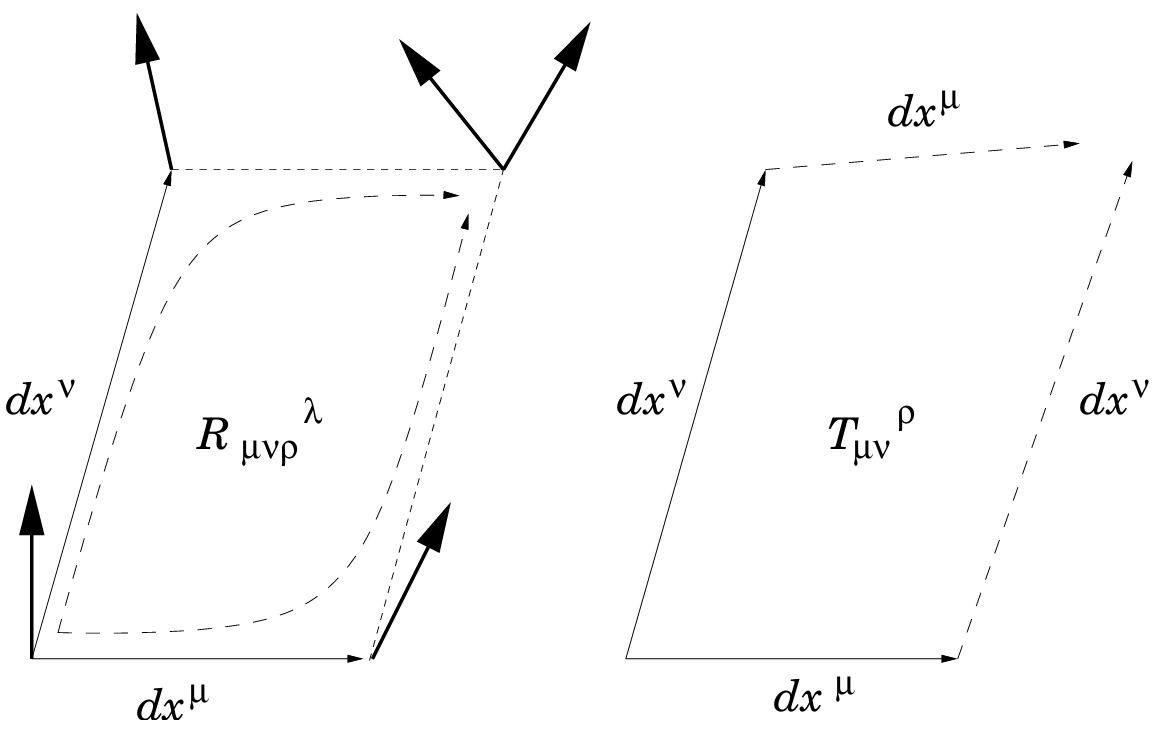
\includegraphics[width=0.6\linewidth]{Figures/riemann tensor and torsion.png}
    \caption{Illustration of parallel transport around an infinitesimal closed loop, showing the deviation of a vector due to curvature, characterized by the Riemann tensor $R^{\lambda}_{\ \mu\nu\rho}$. In the presence of torsion, described by the torsion tensor $T^{\rho}{}_{\mu\nu}$, the infinitesimal parallelogram fails to close, providing a geometric measure of the antisymmetric part of the connection. Source: \cite{LlibreBertJanssen}.}
    \label{fig:riemanntensorparalelogram}
\end{figure}

The commutator of two covariant derivatives acting on a vector field $V^\rho$ is defined by
\begin{equation}
[\nabla_\mu, \nabla_\nu] V^\rho \equiv \nabla_\mu \nabla_\nu V^\rho - \nabla_\nu \nabla_\mu V^\rho.
\end{equation}
Expanding each term in terms of the Christoffel symbols $\Gamma^\rho_{\mu\nu}$, we obtain
\begin{equation}
\nabla_\mu \nabla_\nu V^\rho 
= \partial_\mu (\nabla_\nu V^\rho) 
+ \Gamma^\rho_{\mu\sigma} \nabla_\nu V^\sigma 
- \Gamma^\sigma_{\mu\nu} \nabla_\sigma V^\rho.
\end{equation}
Substituting $\nabla_\nu V^\rho = \partial_\nu V^\rho + \Gamma^\rho_{\nu\lambda} V^\lambda$ into the above, we get
\begin{equation}
\nabla_\mu \nabla_\nu V^\rho 
= \partial_\mu \left( \partial_\nu V^\rho + \Gamma^\rho_{\nu\lambda} V^\lambda \right)
+ \Gamma^\rho_{\mu\sigma} \left( \partial_\nu V^\sigma + \Gamma^\sigma_{\nu\lambda} V^\lambda \right)
- \Gamma^\sigma_{\mu\nu} \left( \partial_\sigma V^\rho + \Gamma^\rho_{\sigma\lambda} V^\lambda \right).
\end{equation}
Expanding the derivatives and rearranging terms, this becomes
\begin{equation}
\begin{aligned}
\nabla_\mu \nabla_\nu V^\rho 
&= \partial_\mu \partial_\nu V^\rho 
+ (\partial_\mu \Gamma^\rho_{\nu\lambda}) V^\lambda 
+ \Gamma^\rho_{\nu\lambda} \partial_\mu V^\lambda\\
& + \Gamma^\rho_{\mu\sigma} \partial_\nu V^\sigma + \Gamma^\rho_{\mu\sigma} \Gamma^\sigma_{\nu\lambda} V^\lambda - \Gamma^\sigma_{\mu\nu} \partial_\sigma V^\rho 
- \Gamma^\sigma_{\mu\nu} \Gamma^\rho_{\sigma\lambda} V^\lambda.
\end{aligned}
\end{equation}
In order to compute the second term of the commutator, we do the same operation, interchanging the indices $(\mu \leftrightarrow \nu)$. 

Finally, we obtain:
\begin{equation}
[\nabla_\mu, \nabla_\nu] V^\rho 
= \left( \partial_\mu \Gamma^\rho_{\nu\sigma} - \partial_\nu \Gamma^\rho_{\mu\sigma} 
+ \Gamma^\rho_{\mu\lambda} \Gamma^\lambda_{\nu\sigma} 
- \Gamma^\rho_{\nu\lambda} \Gamma^\lambda_{\mu\sigma} \right) V^\sigma
- 2\,\Gamma^\lambda_{[\mu\nu]} \, \nabla_\lambda V^\rho.
\end{equation}
The first group of terms corresponds to the components of the Riemann curvature tensor,
\begin{equation}
R^\rho_{\ \sigma\mu\nu} = \partial_\mu \Gamma^\rho_{\nu\sigma} - \partial_\nu \Gamma^\rho_{\mu\sigma} 
+ \Gamma^\rho_{\mu\lambda} \Gamma^\lambda_{\nu\sigma} 
- \Gamma^\rho_{\nu\lambda} \Gamma^\lambda_{\mu\sigma} \ ,
\label{riemanntensoreq}
\end{equation}
while the second term involves the antisymmetric part of the connection,
\begin{equation}
T^\lambda_{\ \mu\nu} = \Gamma^\lambda_{\mu\nu} - \Gamma^\lambda_{\nu\mu} \ ,
\end{equation}
known as the torsion tensor. Since we have already introduced the concept of torsion earlier, we can now give a more precise interpretation: torsion quantifies the failure of an infinitesimal parallelogram to close. Specifically, if the vector $dx^\mu$ is parallel transported along $dx^\nu$ to yield $dx'^\mu$, and $dx^\nu$ is parallel transported along $dx^\mu$ to yield $dx'^\nu$, these two resulting vectors will not, in general, meet at the same point. In other words, the sequence $dx^\mu \rightarrow dx^\nu \rightarrow dx'^\mu \rightarrow dx'^\nu$ does not necessarily form a closed parallelogram. Only for symmetric connections (such as the Levi-Civita connection) does the torsion tensor vanish, ensuring that the paths $dx^\mu$-$dx^\nu$ and $dx^\nu$-$dx^\mu$ yield a closed loop \cite{LlibreBertJanssen}.

When torsion vanishes, only the curvature term remains, providing a direct measure of the manifold's geometric curvature. In this case, the commutator can be expressed compactly as
\begin{equation}
[\nabla_\mu, \nabla_\nu] V^\rho 
= R^\rho_{\ \sigma\mu\nu} V^\sigma - \cancel{T^\lambda_{\ \mu\nu} \nabla_\lambda V^\rho}.
\end{equation}
Thus, the Riemann curvature tensor provides a local, coordinate-independent measure of how much the geometry of a manifold deviates from flatness, encapsulating all such effects within a precise mathematical framework.


\paragraph{Symmetry properties}

The Riemann tensor is antisymmetric in its last two indices:
\begin{equation}
R^\rho_{\ \sigma\mu\nu} = - R^\rho_{\ \sigma\nu\mu} \ ,
\end{equation}
and possesses further symmetries that significantly reduce the number of independent components. In an \(n\)-dimensional manifold, it initially has \(n^4\) components, but these symmetries lower the count to \(1\) in two dimensions, \(6\) in three, and \(20\) in four (as in spacetime geometry).

It is often convenient to express all indices in lowered form using the metric tensor, as this highlights the tensor's symmetry properties in a more transparent way:
\begin{equation}
R_{\alpha\beta\mu\nu} = g_{\alpha\lambda} R^{\lambda}_{\ \beta\mu\nu} \ .
\end{equation}
In this form, the characteristics of $R_{\alpha\beta\mu\nu}$ can be presented as follows:

\begin{itemize}
    \item \textbf{Antisymmetry in each index pair:} The tensor changes sign when the first two indices are swapped, and likewise for the last two:
    \begin{equation}
    R_{\alpha\beta\mu\nu} = - R_{\beta\alpha\mu\nu}, 
    \quad R_{\alpha\beta\mu\nu} = - R_{\alpha\beta\nu\mu} \ .
    \end{equation}
    This means that both $(\alpha,\beta)$ and $(\mu,\nu)$ behave as antisymmetric index pairs.


    \item \textbf{Symmetry under exchange of index pairs:} Interchanging the first and second pair of indices leaves the tensor unchanged:
    \begin{equation}
    R_{\alpha\beta\mu\nu} = R_{\mu\nu\alpha\beta} \ .
    \end{equation}
    This symmetry links curvature measured in one pair of directions to curvature in the orthogonal pair.

    \item \textbf{First Bianchi identity:} The cyclic sum over the last three indices vanishes:
    \begin{equation}
    R_{\alpha\beta\mu\nu} + R_{\alpha\nu\beta\mu} + R_{\alpha\mu\nu\beta} = 0 \ .
    \end{equation}
    This is an algebraic identity that holds in any geometry and reflects fundamental constraints on how curvature can be arranged in a manifold.

\end{itemize}

In the special case of a flat manifold, all curvature components vanish:
\begin{equation}
R^{\alpha}_{\ \beta\mu\nu} = 0 \ ,
\end{equation}
implying that parallel transport is path-independent: any vector transported along a closed curve returns to its starting point unchanged \cite{riemanntensorproperties}.

\subsubsection{Ricci tensor and Ricci scalar}

The complete, uncontracted Riemann curvature tensor does not explicitly appear in EFE. Rather, it is contracted to yield two curvature invariants: the Ricci tensor and the Ricci scalar. These quantities are subsequently combined to construct the Einstein tensor, which forms the geometric side (left-hand side) of EFE \cite{Llibre_Peter_Collier_unacosadificildecomprender}.


\paragraph{Ricci tensor}

By contracting the second index of the Riemann tensor with its fourth index, one obtains the Ricci tensor:
\begin{equation}
R_{\mu\nu} = R_{\ \mu\rho\nu}^{\rho} = g^{\rho\lambda} R_{\mu\rho\nu\lambda} \ .
\end{equation}
Therefore, it is expressed in terms of the connection as follows:
\begin{equation}
R_{\mu\nu} = \partial_{\mu} \Gamma^{\lambda}_{\nu\lambda} - \partial_{\nu} \Gamma^{\lambda}_{\mu\lambda} + \Gamma^{\rho}_{\mu\lambda} \Gamma^{\lambda}_{\nu\rho} - \Gamma^{\rho}_{\nu\lambda} \Gamma^{\lambda}_{\mu\rho} \ .
\end{equation}


\paragraph{Ricci scalar}

By contracting both indices of the Ricci tensor, one obtains the Ricci scalar or curvature scalar:
\begin{equation}
R = R_{\ \mu}^{\mu} = g^{\mu\nu} R_{\mu\nu} \ .
\end{equation}
As the name suggests, the Ricci scalar is a scalar and thus an invariant under general coordinate transformations.


\section{Einstein field equations}

We have now established the necessary mathematical foundations, provided by differential geometry, and complemented them with physical insight from the equivalence principle, allowing us to address EFE. These equations describe how spacetime curvature is determined by the distribution of energy and momentum, offering the precise formulation of gravity in GR. In what follows, we will examine their structure and implications, beginning with intuitive arguments inspired by Einstein’s original reasoning, and then deriving them rigorously from an action principle.


\subsection{The energy-momentun tensor}
\label{The energy-momentun tensor}

We begin by introducing the energy-momentum tensor (also known as the stress-energy tensor), which appears on the right-hand side of EFE. Up to this point, using differential geometry and the equivalence principle, we have interpreted gravity as the curvature of spacetime. However, we have not yet addressed what actually generates that curvature. In Newtonian physics, mass is regarded as the source of the gravitational field.  However, special relativity establishes that the mass of an object is merely one of the possible manifestations of energy, and that it is possible to convert one into the other through the well-known relation \cite{Llibre_Peter_Collier_unacosadificildecomprender}:
\begin{equation}
E^2 = p^2 c^2 + m^2 c^4 \ .
\label{energy-momentum}
\end{equation}
Therefore, it is reasonable to postulate that the source of the gravitational field in GR must encompass not only mass but also energy and momentum. 

Now, we need to find a practical way to represent this source of curvature. This is precisely where the energy-momentum tensor $T^{\mu\nu}$ comes into play. This tensor encapsulates the macroscopic properties of a given physical system, modeled as a fluid\footnote{In GR, all relevant forms of matter can be modeled as perfect fluids (a perfect fluid is one that can be fully characterized solely by its pressure and density), ranging from stars and electromagnetic fields to the entire universe \cite{llibrecarroll2004lectures}.}, including quantities such as velocity, pressure, density, and other relevant parameters, thereby representing the system’s total energy and momentum content. Moreover, the tensor describes the flux of four-momentum \( p^{\mu} \) across a hypersurface of constant \( x^{\nu} \). Therefore we identify \( T^{\mu\nu} \) as the source term in the field equations. 

Since the energy-momentum tensor is a rank-2 tensor, its components can be represented in the form of a \(4 \times 4\) matrix (see Fig.~\ref{fig:energymomentummatrix}).

\begin{figure}[h!]
    \centering
    \hspace{1.9cm}
    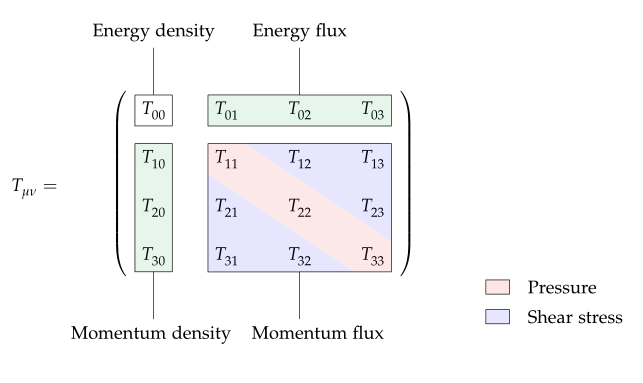
\includegraphics[width=0.7\linewidth]{Figures/energy momentum tensor.png}
    \caption{Schematic representation of the energy-momentum tensor $T_{\mu\nu}$ as a $4 \times 4$ matrix. The components include the energy density ($T_{00}$), energy flux ($T_{0i}$), momentum density ($T_{i0}$), momentum flux ($T_{ij}$), as well as pressure and shear stress terms. Source: \cite{energymomentumtensor}.}
    \label{fig:energymomentummatrix}
\end{figure}

These components can be described as follows:

\begin{itemize}
    \item $T_{00}$ represents the flux of the time component ($\mu=0$) of the four-momentum across a hypersurface of constant $t$ (i.e., normal vector $x^0$). Physically, this corresponds to the energy density in space-time. 
    
    \item $T_{i0} = T_{0i}$ denotes the momentum density (momentum per unit volume) or, equivalently, the energy flux. It can be interpreted as the flow of relativistic mass through a spatial hypersurface with normal vector $x^i$.
    
    \item $T_{ik}$ corresponds to the $i$-th component of the momentum flux through a spatial hypersurface whose normal vector is $x^k$. These terms describe the mechanical stress in the system. When $i = k$, $T_{ii}$ gives the normal stress, which for a static fluid is the isotropic pressure. For $i \neq k$, the components $T_{ik}$ represent shear stresses, related to the fluid's viscosity.
\end{itemize}

The general expression for a perfect fluid in flat spacetime, where 
$g^{\mu\nu} = \eta^{\mu\nu}$, can be written as (using natural units with $c=1$):
\begin{equation}
T^{\mu\nu} = (\rho + P) \, U^{\mu} U^{\nu} \pm P \, \eta^{\mu\nu} \ .
\end{equation}
The choice of sign depends on the metric convention: it is positive for $(-,+,+,+)$ and negative for $(+,-,-,-)$.

Here, $\rho$ denotes the rest-frame energy density, $P$ the isotropic pressure, $\eta^{\mu\nu}$ the Minkowski metric describing flat spacetime (see \cite{derivationenergymomentuntensor} for a derivation), and $U^\mu$ is the four-velocity of the fluid (satisfying $U^\mu U_\mu = -1$ in the $(-,+,+,+)$ metric). The four-velocity takes the form \cite{Llibre_Peter_Collier_unacosadificildecomprender}:
\begin{equation}
U^{\mu} = \left(U^{0}, U^{1}, U^{2}, U^{3}\right) 
= \frac{dx^{\mu}}{d\tau} 
= (c\gamma, \gamma \vec{v}) 
= \gamma (c, \vec{v}) \ .
\end{equation}
Thus, $U^{0} = c\gamma$. In the comoving rest frame, $\gamma = 1$, so we obtain 
$U^{0} = c$ and $U^{0} U^{0} = c^{2}$.

A comoving observer, one who moves together with the fluid and therefore shares its four-velocity $U^\mu$, perceives the fluid as locally isotropic. For such an observer, the four-velocity reduces to $U^{\mu} = (1,0,0,0)$, and the stress-energy tensor simplifies to
\begin{equation}
T^{\mu\nu} = \text{diag}(\rho, P, P, P) \ ,
\end{equation}
assuming the metric $\eta^{\mu\nu} = \text{diag}(-1,1,1,1)$.

To make this more concrete, we now consider a simple example of a perfect fluid.



\subsubsection{Dust or cold matter}

The simplest example of a perfect fluid is cold matter, usually called dust. It is described as a collection of non-interacting particles at rest with respect to each other in a Lorentz frame, or equivalently as a perfect fluid with vanishing pressure \cite{llibrecarroll2004lectures}. Although a realistic dust cloud may swirl in a complicated way, one can always consider a sufficiently small fluid element where the average velocity of the particles is the same.  

With $P=0$, the stress-energy tensor becomes 
\begin{equation}
T^{\mu\nu}_{\text{(dust)}} = \rho \, U^{\mu} U^{\nu} \ ,
\end{equation}
where $\rho$ is the rest-frame energy density \cite{llibretongGR}.  
In the comoving frame of the fluid, with $U^{\mu} = (1,0,0,0)$, the only non-vanishing component is $T^{00} = \rho$, which simply represents the matter density. Hence, non-interacting matter exerts no pressure.



\subsubsection{Conservation of the energy-momentum tensor}

A key property of the energy-momentum tensor is that it satisfies the conservation law \cite{Llibre_Peter_Collier_unacosadificildecomprender}
\begin{equation}
\nabla_\mu T^{\mu\nu} = 0 \ .
\end{equation}
In flat spacetime, this reduces to
\begin{equation}
\partial_\mu T^{\mu\nu} = 0 \ ,
\end{equation}
which encompasses both energy and momentum conservation. By projecting this relation along 
the fluid four-velocity one obtains the relativistic continuity equation (see Appendix $\S$\ref{Derivation of the relativistic continuity and Euler equations} for the derivations),
\begin{equation}
u^\mu \nabla_\mu \rho + (\rho + P)\nabla_\mu u^\mu = 0 \ ,
\end{equation}
expressing the conservation of energy density as the fluid evolves.  

Projecting orthogonally to $u^\mu$ leads instead to the relativistic Euler equation,
\begin{equation}
(\rho + P)u^\mu \nabla_\mu u^\nu = -(g^{\mu\nu} + u^\mu u^\nu)\nabla_\mu P \ ,
\end{equation}
which generalizes Newton’s second law, with pressure gradients acting as the force density \cite{llibretongGR}.  

In curved spacetime the same covariant condition $\nabla_\mu T^{\mu\nu} = 0$ 
remains valid, ensuring that energy and momentum are locally conserved for any 
physically meaningful system.


\subsection{Derivation of the Einstein field equations}

\subsubsection{Heuristic derivation}


Einstein did not reach his field equations in one sudden step of mathematical inspiration, as he sometimes
suggested in his later years, but rather through a gradual process in which physical intuition and formal reasoning worked hand in hand \cite{HowEinsteinfoundhisfieldequations}.

In 1913, together with Marcel Grossmann\footnote{Marcel Grossmann (1878--1936) was a friend, classmate, and early collaborator of Einstein.}, Einstein introduced the Entwurf theory, an early attempt at a relativistic theory of gravitation \cite{EinsteinGrossmann1913}. Its field equations already displayed much of the mathematical framework that would later appear in GR, but they were covariant only under a restricted class of coordinate transformations.

After having established the momentum-energy equation for material processes (mechanical, electrical, and others) in the presence of a gravitational field, Einstein and Grossmann turned to the more fundamental task: to determine the differential equations governing the field itself, namely, the equations for the metric components $g_{ik}$. In analogy with Newton’s theory, they sought a generalization of the Poisson equation
\begin{equation}
\nabla^2 \phi = 4\pi G \rho \ .
\end{equation}
They argued that the field equations should be second order, and proposed that the general form of such equations would be 
\begin{equation}
\kappa \, \Theta_{\mu\nu} = \Gamma_{(\mu\nu)} \ ,
\end{equation}
where $\kappa$ is a coupling constant, $\Theta_{\mu\nu}$ the energy-momentum tensor of matter, and $\Gamma_{\mu\nu}$ a contravariant tensor of second rank constructed from the metric and its derivatives \cite{howeinsteinfoundhisequations}. Although this construction ensured the conservation of energy and momentum, the resulting equations were not generally covariant, but only valid under linear transformations. Einstein himself emphasized that it was not possible, at that stage, to obtain second-order equations that were simultaneously a true generalization of the Laplacian and a tensor under arbitrary coordinate changes.

The Entwurf theory thus represented a crucial but incomplete step. It incorporated the basic dynamical structure of GR covariance. Over the following two years Einstein gradually moved beyond it. In November 1915 he presented to the Prussian Academy a sequence of communications (see Section $\S$\ref{Einstein's journey to general relativity}) in which he successively improved the covariance and physical adequacy of his field equations. 

First, he proposed
\begin{equation}
R_{\mu\nu} = -\kappa T_{\mu\nu} \ ,
\end{equation}
equations that were valid under unimodular transformations\footnote{A unimodular transformation is a coordinate transformation whose Jacobian determinant equals 1, that is,
\begin{equation}
\det \left( \frac{\partial x'^\mu}{\partial x^\nu} \right) = 1 \ .
\end{equation}
This means the coordinate change preserves volume, so the volume element $d^4x$ remains unchanged \cite{unimodular_transf}.}, giving them broader covariance than the Entwurf equations, but they
still fell short of full generality. A week later he introduced the additional condition
\begin{equation}
T \equiv g^{\mu\nu} T_{\mu\nu} = 0 \ ,
\end{equation}
which allowed him to reinterpret the equations as generally covariant. With this version he was already able to account for the anomalous precession of Mercury’s perihelion, $\Delta \varphi \approx 43'' \ \text{per century}$ (see \cite{precession} for more details), a striking empirical success. Yet the restriction $T=0$ was too severe to be acceptable in general.

The decisive step came on 25 November 1915, when Einstein realized that adding an explicit trace term to the right-hand side of the field equations would remove the need for this artificial constraint. The final generally covariant field equations took the form
\begin{equation}
R_{\mu\nu} - \tfrac{1}{2} g_{\mu\nu} R = \kappa T_{\mu\nu} \ ,
\end{equation}
where $R_{\mu\nu}$ is the Ricci tensor, $R$ the Ricci scalar, $g_{\mu\nu}$ the metric tensor, and $T_{\mu\nu}$ the energy-momentum tensor of matter and fields. The constant $\kappa = 8\pi G / c^4$ ensures consistency with Newton’s theory in the weak-field limit (see Appendix $\S$\ref{Appendix:Einstein field equations (Newtonian limit)} for the derivation).

It is important to note that while the Ricci tensor and the metric tensor were already known from the work of Gregorio Ricci-Curbastro and Tullio Levi-Civita in the context of differential geometry, the specific combination appearing on the left-hand side, known today as the Einstein tensor $G_{\mu\nu} \equiv R_{\mu\nu} - \tfrac{1}{2} g_{\mu\nu} R$, was formulated by Einstein in 1915 \cite{llibretheoreticalminimum}. This tensor was designed to have zero covariant divergence, $\nabla^\mu G_{\mu\nu} = 0$, ensuring consistency with the local conservation of energy and momentum and making it the natural choice to relate spacetime curvature to the energy-momentum content.



Einstein's equations constitute a system of ten coupled, second-order nonlinear partial differential equations, which makes them extremely challenging to solve analytically. No general method is known, and the solutions that have been obtained usually rely on assuming a high degree of symmetry or on applying specialized techniques (see Section $\S$\ref{solutionseinsteinequations}). 

Although Einstein's equations formally involve ten components, the condition $\nabla_\mu G^{\mu\nu} = 0$ provides four constraints, leaving only six equations that are genuinely independent. This implies that, out of the ten components of the metric, only six are determined by Einstein's equations and correspond to physical degrees of freedom. The remaining four are non-physical components that express the freedom in the choice of coordinates \cite{LlibreBertJanssen}.

\subsubsection{Formal derivation from the Einstein-Hilbert action}


We will now derive EFE starting from the Einstein-Hilbert action. Although this is not the original method used by Einstein, it provides a more modern and elegant approach, as it is based on the principle of least action. This formulation is particularly useful since the principle of least action plays a central role in theoretical physics.

For clarity, the derivation will be presented step by step, as carrying it out all at once can be rather difficult to follow.

We begin by considering the variation of the square root of the negative determinant of the metric tensor ($\S$\ref{Variation_of_the_squareroot}), a quantity that will play a crucial role in our derivation. Next, we will compute the contraction of the Christoffel symbols ($\S$\ref{Contraction_Christoffelsymbol}), followed by the variation of the Ricci scalar ($\S$\ref{Variation_Ricciscalar}). Finally, we will obtain the variation of the Einstein-Hilbert action itself ($\S$\ref{Variation_of_Hilbert_Einstein_action}).

Before proceeding with these steps, we first define the Einstein-Hilbert action.


\paragraph{Einstein-Hilbert action}
\label{Einstein--Hilbert action}


From analytical mechanics we know the advantages of the Lagrangian formulation: by varying with 
respect to the system's degrees of freedom one directly obtains the equations of motion. In this sense, 
the Lagrangian provides a compact representation of the dynamics of a system or a theory. Moreover, in many cases it is more straightforward to identify the symmetries of a system through its Lagrangian rather than directly from the equations of motion. For instance, the trajectory of a free particle in a curved spacetime can be derived from an action principle, leading to the geodesic equation \eqref{geodesicequation} \cite{LlibreBertJanssen}. 

It is therefore natural to ask whether gravity itself can be described by an action. The answer is provided by the Einstein-Hilbert action, which yields EFE in vacuum and is expressed as (see Appendix $\S$\ref{Appendix Einstein-Hilbert action} for the derivation)
\begin{equation}
S_{EH} = \frac{c^4}{16 \pi G} \int_{\mathcal{M}} d^4x \, \sqrt{-g} \, R \ ,
\end{equation}
where $g = \det(g_{\mu\nu})$ is the determinant of the metric and $R$ is the Ricci scalar. The minus sign inside the square root appears because the underlying spacetime is Lorentzian: the metric possesses one negative eigenvalue, which makes its determinant 
$g = \det(g_{\mu\nu})$ negative \cite{llibretongGR}.

In this way, the Einstein-Hilbert action plays for GR the same role that the Lagrangian 
does in analytical mechanics: it encodes the dynamics of the gravitational field in a compact and elegant form.



\paragraph{Variation of the square root of the negative determinant of the metric}
\label{Variation_of_the_squareroot}

We begin by deriving the variation of the determinant of the metric tensor.


First, let us consider a mathematical note.  
Take the following function of two variables and expand it in a first-order Taylor series:
\begin{equation}
f(x,y) = \sqrt{xy} \;\;\;\Rightarrow\;\;\;
f(x,y) \simeq f(x_0,y_0) 
+ \left.\frac{\partial f}{\partial x}\right|_{(x_0,y_0)} (x-x_0) 
+ \left.\frac{\partial f}{\partial y}\right|_{(x_0,y_0)} (y-y_0) \ .
\end{equation}
The derivatives are given by
\begin{equation}
\frac{\partial f}{\partial x} = \frac{y}{2\sqrt{xy}} \ , 
\qquad 
\frac{\partial f}{\partial y} = \frac{x}{2\sqrt{xy}} \ .
\end{equation}
Therefore, we obtain
\begin{equation}
\sqrt{xy} \;\simeq\; \sqrt{x_0 y_0} + \frac{1}{2\sqrt{x_0 y_0}}
\Big[ y_0 (x-x_0) + x_0 (y-y_0) \Big] \ .
\end{equation}
We now define the variation of a function $\delta f$ as the difference between its values at two different points:
\begin{equation}
\delta(\sqrt{xy}) = \sqrt{xy} - \sqrt{x_0 y_0}
= \frac{1}{2\sqrt{x_0 y_0}} \Big[ y_0 \, \delta x + x_0 \, \delta y \Big]
= \frac{\sqrt{x_0 y_0}}{2} \left( \frac{\delta x}{x_0} + \frac{\delta y}{y_0} \right) \ .
\end{equation}
More generally, if we consider the square root of a product of $n$ variables, it can be shown by induction that
\begin{equation}
\delta\!\left(\sqrt{x_1 x_2 x_3 \cdots x_n}\right) 
= \frac{\sqrt{x_1 x_2 \cdots x_n}}{2} 
\sum_{i=1}^n \frac{\delta x_i}{x_i} \ .
\end{equation}
Let us now apply this idea to matrices.  
Consider a symmetric matrix $A$ with $\det A > 0$. We know that:
\begin{enumerate}
    \item $A$ is diagonalizable.
    \item Consequently, there exists a basis such that
    \begin{equation}
    A = \mathrm{diag}(\lambda_1, \lambda_2, \dots, \lambda_n) \ , 
    \qquad \lambda_i \in \mathbb{R} \ .
    \end{equation}
    \item The determinant of $A$ is invariant under a change of basis, that is
    \begin{equation}
    \det A = \lambda_1 \lambda_2 \cdots \lambda_n \ .
    \end{equation}
\end{enumerate}
Therefore, the variation reads
\begin{equation}
\delta(\sqrt{\det A}) = \frac{\sqrt{\det A}}{2} 
\sum_{i=1}^n \frac{\delta \lambda_i}{\lambda_i}.
\end{equation}
Using the metric tensor, we obtain
\begin{equation}
\delta(\sqrt{\det g}) = \frac{\sqrt{\det g}}{2} 
\left( \frac{1}{g_{11}} \delta g_{11} + \frac{1}{g_{22}} \delta g_{22} \right)
= \frac{\sqrt{\det g}}{2} \, g^{\alpha\beta} \, \delta g_{\alpha\beta} \ .
\end{equation}
A potential concern is whether this expression remains valid for both diagonal and non-diagonal metrics, since in the latter case $\tfrac{1}{g_{ij}} \neq g^{ij}$ for $i \neq j$.  
The answer is yes: the expression holds in general. The reason is that both $g^{\alpha\beta}$ and $g_{\alpha\beta}$ are tensors, and their variations are also tensors. Thus, the contraction $g^{\alpha\beta}\delta g_{\alpha\beta}$ is a scalar, valid in any basis.


Finally, writing $\det g \equiv g$, we obtain
\begin{equation}
\delta(\sqrt{g}) = \frac{\sqrt{g}}{2}\, g^{\alpha\beta}\, \delta g_{\alpha\beta} \ , 
\qquad g>0 \ ,
\end{equation}
\begin{equation}
\delta(\sqrt{-g}) = \frac{\sqrt{-g}}{2}\, g^{\alpha\beta}\, \delta g_{\alpha\beta} \ , 
\qquad g<0 \ .
\label{variationofmetric}
\end{equation}

This result is one of the fundamental steps in deriving EFE \cite{Garcia2019RelativityCourse}.



\paragraph{Contraction of the Christoffel symbol}
\label{Contraction_Christoffelsymbol}

We want to prove the following identity:
\begin{equation}
\Gamma^\mu_{\mu\nu} = \frac{1}{\sqrt{-g}} \, \partial_\nu \sqrt{-g} \ .
\label{contractionchristoffelsymbols}
\end{equation}
This result will be very useful in subsequent derivations.  


Recall the definition of the Christoffel symbols:
\begin{equation}
\Gamma^\mu_{\mu\nu} = \frac{1}{2} g^{\mu\rho} 
\left( \partial_\nu g_{\rho\mu} + \partial_\mu g_{\rho\nu} - \partial_\rho g_{\mu\nu} \right) \ .
\end{equation}
Expanding, we obtain
\begin{equation}
\Gamma^\mu_{\mu\nu} 
= \frac{1}{2} \Big( g^{\mu\rho} \, \partial_\nu g_{\rho\mu} 
+ g^{\mu\rho} \, \partial_\mu g_{\rho\nu} 
- g^{\mu\rho} \, \partial_\rho g_{\mu\nu} \Big) \ .
\end{equation}
Changing dummy indices in the last two terms, we rewrite this expression as
\begin{equation}
\Gamma^\mu_{\mu\nu} 
= \frac{1}{2} \Big( g^{\mu\rho} \, \partial_\nu g_{\rho\mu} 
+ g^{\mu\rho} \, \partial_\mu g_{\rho\nu} 
- g^{\rho\mu} \, \partial_\mu g_{\rho\nu} \Big) \ .
\end{equation}
Since the metric tensor is symmetric, $g^{\mu\rho} = g^{\rho\mu}$, the last two terms cancel. Thus we obtain
\begin{equation}
\Gamma^\mu_{\mu\nu} = \frac{1}{2} g^{\mu\rho} \, \partial_\nu g_{\rho\mu} \ .
\end{equation}
Now, recall the variation of $\sqrt{-g}$ obtained previously in \eqref{variationofmetric}.  
Dividing both sides of that expression by $\delta x^\nu$, we have
\begin{equation}
\frac{\delta \sqrt{-g}}{\delta x^\nu} 
= \frac{1}{2} \sqrt{-g}\, g^{\alpha\beta} \, \frac{\delta g_{\alpha\beta}}{\delta x^\nu} \ .
\end{equation}
In the infinitesimal limit, this becomes
\begin{equation}
\frac{\partial \sqrt{-g}}{\partial x^\nu} 
= \frac{1}{2} \sqrt{-g}\, g^{\alpha\beta} \, \frac{\partial g_{\alpha\beta}}{\partial x^\nu} \ .
\end{equation}
Therefore, dividing through by $\sqrt{-g}$, we obtain
\begin{equation}
\frac{1}{\sqrt{-g}} \, \partial_\nu \sqrt{-g} 
= \frac{1}{2} g^{\alpha\beta} \, \partial_\nu g_{\alpha\beta} 
= \Gamma^\mu_{\mu\nu} \ .
\end{equation}
This proves the desired identity \cite{cursoJavierGarcia53}.


\paragraph{Variation of the Ricci scalar}
\label{Variation_Ricciscalar}


Let us recall the expression for the Ricci tensor:
\begin{equation}
R_{\sigma \nu} = \partial_\mu \Gamma^{\mu}_{\nu \sigma} - \partial_\nu \Gamma^{\mu}_{\mu \sigma} 
+ \Gamma^{\mu}_{\mu \lambda} \Gamma^{\lambda}_{\nu \sigma} 
- \Gamma^{\mu}_{\nu \lambda} \Gamma^{\lambda}_{\mu \sigma} \ .
\end{equation}
We will use the elementary variation properties
\begin{enumerate}
    \item $\delta(A \cdot B) = (\delta A) B + A (\delta B) \ ,$
    \item $\delta(\partial A) = \partial (\delta A) \ .$
\end{enumerate}
We compute the variation of $R_{\sigma \nu}$:
\begin{equation}
\delta R_{\sigma \nu} = \partial_\mu (\delta \Gamma^{\mu}_{\nu \sigma}) - \partial_\nu (\delta \Gamma^{\mu}_{\mu \sigma})
+ \Gamma^{\mu}_{\mu \lambda} (\delta \Gamma^{\lambda}_{\nu \sigma})
+ (\delta \Gamma^{\mu}_{\mu \lambda}) \Gamma^{\lambda}_{\nu \sigma}
- \Gamma^{\mu}_{\nu \lambda} (\delta \Gamma^{\lambda}_{\mu \sigma})
- (\delta \Gamma^{\mu}_{\nu \lambda}) \Gamma^{\lambda}_{\mu \sigma} \ .
\end{equation}
Although the Christoffel symbols $\Gamma^{\lambda}{}_{\rho \sigma}$ are not tensorial, their variation is tensorial; hence we define:
\begin{equation}
T^{\lambda}_{\ \rho \sigma} \equiv \delta \Gamma^{\lambda}_{\rho \sigma}.
\end{equation}
With this notation, the previous result becomes
\begin{equation}
\delta R_{\sigma \nu}
= \partial_\mu T^{\mu}{}_{\nu \sigma}
- \partial_\nu T^{\mu}{}_{\mu \sigma}
+ \Gamma^{\mu}{}_{\mu \lambda}\, T^{\lambda}{}_{\nu \sigma}
+ T^{\mu}{}_{\mu \lambda}\, \Gamma^{\lambda}{}_{\nu \sigma}
- \Gamma^{\mu}{}_{\nu \lambda}\, T^{\lambda}{}_{\mu \sigma}
- T^{\mu}{}_{\nu \lambda}\, \Gamma^{\lambda}{}_{\mu \sigma} \, .
\end{equation}
We now rewrite these terms using covariant derivatives of the tensor $T^{\lambda}{}_{\rho \sigma}$,
\begin{equation}
\nabla_\rho T^{\lambda}{}_{\sigma \nu}
= \partial_\rho T^{\lambda}{}_{\sigma \nu}
+ \Gamma^{\lambda}{}_{\rho \alpha}\, T^{\alpha}{}_{\sigma \nu}
- \Gamma^{\alpha}{}_{\rho \sigma}\, T^{\lambda}{}_{\alpha \nu}
- \Gamma^{\alpha}{}_{\rho \nu}\, T^{\lambda}{}_{\sigma \alpha} \, .
\end{equation}
In particular, we have
\begin{equation}
\nabla_\mu T^{\mu}{}_{\nu \sigma}
= \partial_\mu T^{\mu}{}_{\nu \sigma}
+ \Gamma^{\mu}{}_{\mu \alpha}\, T^{\alpha}{}_{\nu \sigma}
- \Gamma^{\alpha}{}_{\mu \nu}\, T^{\mu}{}_{\alpha \sigma}
- \Gamma^{\alpha}{}_{\mu \sigma}\, T^{\mu}{}_{\nu \alpha} \, ,
\end{equation}
and
\begin{equation}
\nabla_\nu T^{\mu}{}_{\mu \sigma}
= \partial_\nu T^{\mu}{}_{\mu \sigma}
+ \Gamma^{\mu}{}_{\nu \alpha}\, T^{\alpha}{}_{\mu \sigma}
- \Gamma^{\alpha}{}_{\nu \mu}\, T^{\mu}{}_{\alpha \sigma}
- \Gamma^{\alpha}{}_{\nu \sigma}\, T^{\mu}{}_{\mu \alpha} \, .
\end{equation}
Subtracting the last two relations reproduces the variation of the Ricci tensor in a compact form,
\begin{equation}
\delta R_{\sigma \nu}
= \nabla_\mu T^{\mu}{}_{\nu \sigma}
- \nabla_\nu T^{\mu}{}_{\mu \sigma} \, , \qquad
\text{with  } T^{\lambda}{}_{\rho \sigma} \equiv \delta \Gamma^{\lambda}{}_{\rho \sigma} \, .
\end{equation}
This is the Palatini identity \cite{cursoJavierGarcia54},
\begin{equation}
\delta R_{\sigma \nu}
= \nabla_\mu \bigl(\delta \Gamma^{\mu}{}_{\nu \sigma}\bigr)
 - \nabla_\nu \bigl(\delta \Gamma^{\mu}{}_{\mu \sigma}\bigr) \, .
 \label{Palatini identity}
\end{equation}
With this result, we can now compute the variation of the scalar curvature, also referred to as the Ricci scalar.

The scalar curvature is defined as
\begin{equation}
R = g^{\alpha \beta} R_{\alpha \beta} \, .
\end{equation}
Therefore, its variation is
\begin{equation}
\delta R = \delta(g^{\alpha \beta}) R_{\alpha \beta} + g^{\alpha \beta}\, \delta R_{\alpha \beta} \, .
\end{equation}
Using the Palatini identity \eqref{Palatini identity}, we write
\begin{equation}
\delta R = \delta(g^{\alpha \beta}) R_{\alpha \beta}
+ g^{\alpha \beta} \left( \nabla_{\lambda} \delta \Gamma^{\lambda}{}_{\beta \alpha}
- \nabla_{\beta} \delta \Gamma^{\lambda}{}_{\lambda \alpha} \right) \, .
\end{equation}
Since the covariant derivative of the metric vanishes,
\(\nabla_{\mu} g^{\alpha \beta} = 0\),
we can rewrite the divergence term as
\begin{equation}
\nabla_{\lambda} \bigl( g^{\alpha \beta} \, \delta \Gamma^{\lambda}{}_{\beta \alpha} \bigr)
= \cancel{(\nabla_{\lambda} g^{\alpha \beta}) \, \delta \Gamma^{\lambda}{}_{\beta \alpha}}
+ g^{\alpha \beta} \nabla_{\lambda} \delta \Gamma^{\lambda}{}_{\beta \alpha} \, ,
\end{equation}
where the first contribution vanishes due to metric compatibility.


Thus, the expression simplifies to
\begin{equation}
\delta R = R_{\alpha \beta} \, \delta g^{\alpha \beta}
+ \nabla_{\lambda} \bigl( g^{\alpha \beta} \, \delta \Gamma^{\lambda}{}_{\beta \alpha} \bigr)
- \nabla_{\beta} \bigl( g^{\alpha \beta} \, \delta \Gamma^{\lambda}{}_{\lambda \alpha} \bigr) \, .
\end{equation}
By relabeling the dummy index $\lambda$ as $\mu$ in the second term and 
$\beta$ as $\mu$ in the third term, we obtain
\begin{equation}
\delta R = R_{\alpha \beta}\, \delta g^{\alpha \beta}
+ \nabla_{\mu} \left( g^{\alpha \beta} \, \delta \Gamma^{\mu}{}_{\beta \alpha}
- g^{\alpha \mu} \, \delta \Gamma^{\lambda}{}_{\lambda \alpha} \right) \, .
\end{equation}
Defining the vector
\begin{equation}
J^{\mu} \equiv g^{\alpha \beta} \, \delta \Gamma^{\mu}{}_{\beta \alpha}
- g^{\alpha \mu} \, \delta \Gamma^{\lambda}{}_{\lambda \alpha} \, ,
\end{equation}
which transforms as a tensor, we obtain the compact result
\begin{equation}
\delta R = R_{\alpha \beta}\, \delta g^{\alpha \beta} + \nabla_{\mu} J^{\mu} \, .
\label{variationricciscalar}
\end{equation}


\paragraph{Variation of the Hilbert-Einstein action}
\label{Variation_of_Hilbert_Einstein_action}


Now we can compute the variation of the Einstein-Hilbert action:
\begin{align}
\delta S_{EH} &= \delta \int d^4x \, \sqrt{-g}\, R 
= \int d^4x \, \delta \!\left(\sqrt{-g}\, R\right) \\
&= \int d^4x \Big[\left(\delta\sqrt{-g}\right) R + \sqrt{-g}\, \delta R \Big].
\end{align}

Now, using the relations \eqref{variationofmetric} and \eqref{variationricciscalar} we get
\begin{align}
\delta S 
&= \int d^4x \Big[ \Big(\tfrac{1}{2}\sqrt{-g}\, g^{\alpha\beta} \delta g_{\alpha\beta}\Big) R 
+ \sqrt{-g}\, \big( R_{\alpha\beta}\, \delta g^{\alpha\beta} + \nabla_\mu J^\mu \big) \Big],
\end{align}
where the last term is a total divergence.

Applying the principle of least action, we write
\begin{align}
\delta S &= \int d^4x \, \frac{\sqrt{-g}}{2} R\, g^{\alpha\beta} \delta g_{\alpha\beta} 
+ \int d^4x \, \sqrt{-g}\, R_{\alpha\beta}\, \delta g^{\alpha\beta}
+ \int d^4x \, \sqrt{-g}\, \nabla_\mu J^\mu = 0.
\end{align}
The divergence term can be expressed as
\begin{equation}
\begin{aligned}
\nabla_\mu J^\mu 
&= \partial_\mu J^\mu + \Gamma^{\mu}_{\lambda \mu}\, J^\lambda \\
&= \partial_\mu J^\mu + \frac{1}{\sqrt{-g}} (\partial_\lambda\sqrt{-g}) J^\lambda \\
&= \frac{1}{\sqrt{-g}} \Big[ \sqrt{-g}\, \partial_\mu J^\mu + (\partial_\lambda \sqrt{-g}) J^\lambda \Big] \\
&= \frac{1}{\sqrt{-g}} \, \partial_\lambda(\sqrt{-g}\, J^\lambda) \ ,
\end{aligned}
\end{equation}
where we have used the relation \eqref{contractionchristoffelsymbols} and we have relabeled the dummy index $\mu$ as $\lambda$.

Therefore,
\begin{align}
\delta S_{EH} &= \int d^4x \, \frac{\sqrt{-g}}{2} R\, g^{\alpha\beta}\, \delta g_{\alpha\beta} 
+ \int d^4x \, \sqrt{-g}\, R_{\alpha\beta}\, \delta g^{\alpha\beta} 
+ \int d^4x \, \partial_\lambda(\sqrt{-g}\, J^\lambda) \ .
\end{align}


The last term is a surface contribution. For compact manifolds without boundary, this term vanishes identically and will therefore be set to zero in this thesis.
In contrast, for spacetimes with a boundary it does not vanish, and in order to make the Einstein-Hilbert action well-defined under metric variations, one must add the Gibbons-Hawking-York boundary term.

This additional piece is constructed from the trace of the extrinsic curvature of the boundary, denoted by $K$, and modifies the action in the following way \cite{BoundaryTerms}:
\begin{equation}
S = S_{EH} + S_{GHY} \;\sim\; \int_{\mathcal{M}} d^{4}x\,\sqrt{-g}\,R \;+\; 2 \int_{\mathcal{\partial M}} d^{3}x\,\sqrt{|h|}\,K \ ,
\end{equation}
where $h$ stands for the determinant of the induced metric on the boundary. Further discussion can be found in \cite{cursoJavierGarcia57}.



Now we are interested in factoring out the variation of the metric. 
However, in the first term the indices appear lowered, while in the second term they appear raised. 
Therefore, we need to employ a useful trick that allows us to raise the indices in the variation of the metric. 

We start from the identity
\begin{equation}
g_{\alpha\beta} g^{\beta\gamma} = \delta_\alpha^\gamma,
\end{equation}
its variation yields
\begin{equation}
\delta\!\left(g_{\alpha\beta} g^{\beta\gamma}\right) = 0 
= \left(\delta g_{\alpha\beta}\right) g^{\beta\gamma} 
+ g_{\alpha\beta}\, \delta g^{\beta\gamma},
\end{equation}
which implies
\begin{equation}
g^{\beta\gamma}(\delta g_{\alpha\beta})= - g_{\alpha\beta}\delta g^{\beta\gamma} \ .
\end{equation}

Taking the trace of a tensor $T^\mu{}_\nu$ gives
\begin{equation}
\mathrm{Tr}\, T^\mu{}_\nu = T^0{}_0 + T^1{}_1 + T^2{}_2 + T^3{}_3 = T^\mu{}_\mu \ .
\end{equation}
Applying this to the metric variation, we obtain
\begin{equation}
Tr\Big[ g^{\beta\gamma}(\delta g_{\alpha\beta})= - g_{\alpha\beta}\delta g^{\beta\gamma}\Big]\;\;\;\Rightarrow\;\;\;
g^{\alpha\beta} \left(\delta g_{\alpha\beta}\right) = - g_{\alpha\beta} \, \delta g^{\alpha\beta},
\end{equation}
where we have used the symmetry of the metric tensor $g^{\beta\alpha}=g^{\alpha\beta}$.

Thus, the variation of the Einstein-Hilbert action can be written as
\begin{equation}
\delta S 
= \int d^4x \left[ -\tfrac{1}{2}\sqrt{-g}\, g_{\alpha\beta} R \, \delta g^{\alpha\beta} 
+ \sqrt{-g}\, R_{\alpha\beta}\, \delta g^{\alpha\beta} \right] .
\end{equation}
Therefore, imposing $\delta S = 0$, we obtain
\begin{equation}
\delta S 
= \int d^4x \, \sqrt{-g} 
\left(R_{\alpha\beta} - \tfrac{1}{2} g_{\alpha\beta} R \right)\delta g^{\alpha\beta} = 0.
\end{equation}
Since the variations $\delta g^{\alpha\beta}$ are arbitrary, this yields the EFE in vacuum:
\begin{equation}
G_{\alpha\beta} := R_{\alpha\beta} - \tfrac{1}{2} g_{\alpha\beta} R = 0.
\end{equation}

In order to include matter fields in the theory, we add an additional term to the gravitational action. The total action then takes the form
\begin{equation}
    S = S_{EH} + S_{GHY} + S_M  = \frac{c^4}{16 \pi G}\int_{\mathcal{M}} d^{4}x\,\sqrt{-g}\,R \;+\; \frac{c^4}{8 \pi G} \int_{\mathcal{\partial M}} d^{3}x\,\sqrt{|h|}\,K + \int_{\mathcal{M}} d^{4}x\,\sqrt{-g}\,\mathcal{L_\text{m}} \ ,
\end{equation}
where $\mathcal{L}_{m}$ denotes the matter Lagrangian density.

We now consider the variation of the total action 
\begin{equation}
\delta S = \frac{c^4}{16 \pi G} \int d^{4}x \, \sqrt{-g}\, \delta g^{\alpha\beta}
\left( R_{\alpha\beta} - \tfrac{1}{2} g_{\alpha\beta} R \right)
+ \delta \left( \int d^{4}x \, \sqrt{-g}\, \mathcal{L}_{m} \right)  .
\end{equation}
The variation of the matter action reads
\begin{equation}
\delta S_{m} = \int d^{4}x \, \delta\!\left(\sqrt{-g}\, \mathcal{L}_{m}\right) 
= \int d^{4}x \left[ (\delta\sqrt{-g})\, \mathcal{L}_{m} + \sqrt{-g}\, \delta \mathcal{L}_{m} \right] \, .
\end{equation}
Since the variation of the determinant is
\begin{equation}
\delta(\sqrt{-g}) = -\tfrac{1}{2} \sqrt{-g}\, g_{\alpha\beta}\, \delta g^{\alpha\beta} \, ,
\end{equation}
and the variation of the matter Lagrangian can be expressed as
\begin{equation}
\delta \mathcal{L}_{m} = \frac{\delta \mathcal{L}_{m}}{\delta g^{\alpha\beta}} \, \delta g^{\alpha\beta} \, ,
\end{equation}
the full variation of the matter action becomes
\begin{equation}
\delta S_{m} = \int d^{4}x \, \tfrac{1}{2}\sqrt{-g} \, \delta g^{\alpha\beta} 
\left[ - g_{\alpha\beta} \mathcal{L}_{m} \,  
+ \frac{\delta \mathcal{L}_{m}}{\delta g^{\alpha\beta}} \right] \, .
\end{equation}
Gathering all contributions, the total variation of the action reads
\begin{equation}
\delta S = \int d^{4}x \, \sqrt{-g}\,\delta g^{\alpha\beta} 
\left[ \frac{c^4}{16 \pi G} \left( R_{\alpha\beta} - \tfrac{1}{2} g_{\alpha\beta} R \right) 
+ \tfrac{1}{2} \Big(-g_{\alpha\beta} \mathcal{L}_{m} 
+ 2\frac{\partial \mathcal{L}_{m}}{\partial g^{\alpha\beta}}\Big) \right] \ .
\end{equation}
Applying the variational principle considering $\delta S = 0$ we obtain:
\begin{equation}
     R_{\alpha\beta} - \tfrac{1}{2} g_{\alpha\beta} R  
= -\frac{8 \pi G}{c^4} \Big(-g_{\alpha\beta} \mathcal{L}_{m} 
+ 2\frac{\partial \mathcal{L}_{m}}{\partial g^{\alpha\beta}}\Big). 
\end{equation}
Identifying the energy-momentum tensor as
\begin{equation}
T_{\alpha\beta} = g_{\alpha\beta} \, \mathcal{L}_{m} - 2 \frac{\partial \mathcal{L}_{m}}{\partial g^{\alpha\beta}} 
 = \frac{-2}{\sqrt{-g}} 
\frac{\delta (\sqrt{-g}\,\mathcal{L}_{m})}{\delta g^{\alpha\beta}} \ ,
\end{equation}
we finally obtain the EFE in the form
\begin{equation}
R_{\alpha\beta} - \tfrac{1}{2} g_{\alpha\beta} R 
= \frac{8\pi G}{c^{4}}\, T_{\alpha\beta} \, .
\end{equation}


\subsection{The cosmological constant}


So far we have justified EFE in two distinct ways: first, as the natural covariant extension of Poisson’s equation for the Newtonian potential; and second, as the outcome of varying the simplest possible action constructed from the metric. Before exploring explicit solutions, it is instructive to examine possible modifications of these equations. Among the many conceivable generalizations, a particularly important one is the introduction of a cosmological constant $\Lambda$ \cite{llibrecarroll2004lectures}.

The action is then modified to include this additional contribution,
\begin{equation}
S = -\frac{c^{4}}{16\pi G} \int d^{4}x \, \sqrt{-g}\,(R - 2\Lambda) 
+ \int d^{4}x \, \sqrt{-g}\,\mathcal{L}_{m} \, ,
\end{equation}
which leads to the field equations
\begin{equation}
R_{\alpha\beta} - \tfrac{1}{2} g_{\alpha\beta} R + g_{\alpha\beta}\Lambda 
= \frac{8 \pi G}{c^{4}}\, T_{\alpha\beta} \, .
\label{einsteinequations}
\end{equation}
Historically, Einstein introduced the cosmological constant in 1917 as a way to obtain a static universe without beginning or end, effectively behaving like a repulsive or ``antigravitational'' pressure. However, soon after, it was realized that the static solutions of the field equations were unstable. In 1929, the American astronomer Edwin Hubble (1889--1953) discovered that the universe is in fact expanding, a result fully consistent with the original, unmodified field equations. This led Einstein to famously refer to the cosmological constant as ``the biggest blunder'' of his life.  

Ironically, observations in 1998 with the Hubble Space Telescope revealed that the universe is not only expanding but doing so at an accelerated rate. One possible explanation invokes a pervasive dark energy that fills space and may be effectively described by the cosmological constant. Thus, what Einstein once dismissed as his greatest mistake has regained scientific relevance: dark energy and the cosmological constant now appear essential to account for the accelerated expansion of the universe, even though their true physical nature remains one of the deepest mysteries in modern physics \cite{Llibre_Peter_Collier_unacosadificildecomprender}.



The modern challenge, however, lies in the so-called cosmological constant problem: the theoretical estimates of $\Lambda$ obtained from quantum field theory suggest a natural scale of order $\Lambda \sim m_{P}^{4} \sim 10^{76}\,\mathrm{GeV}^{4}$, while cosmological observations constrain it to be about $10^{-47}\,\mathrm{GeV}^{4}$. This discrepancy of roughly $10^{123}$ is the largest known mismatch between theory and experiment, making the cosmological constant one of the deepest unresolved puzzles in contemporary physics \cite{LlibreBertJanssen}.

\section{Relevant solutions to Einstein’s equations}
\label{solutionseinsteinequations}

EFE are extremely challenging to solve because of their intrinsic nonlinearity. Unlike linear systems, the superposition of two independent solutions does not in general produce a new one. The physical origin of this nonlinearity is simple: spacetime curvature is generated by the presence of matter and energy, yet the curvature itself carries energy and momentum, thereby acting as an additional source of curvature. In other words, gravity is not only coupled to matter and energy but also to itself, which makes the field equations nonlinear by nature.

Concretely, to “find a solution” means to determine a metric tensor $g_{\mu\nu}$ (and, when relevant, a compatible matter configuration) that satisfies
\[
R_{\mu\nu}-\tfrac{1}{2}g_{\mu\nu}R+\Lambda g_{\mu\nu}=\frac{8\pi G}{c^{4}}\,T_{\mu\nu},
\]
subject to appropriate boundary or initial conditions.

Each solution corresponds to a possible spacetime geometry associated with a particular distribution of matter and energy. Broadly speaking, they can be grouped into three categories: 
\begin{itemize}
    \item \textbf{Exact analytical solutions}: such as the Schwarzschild, Kerr, or Friedmann-Lemaître-Robertson-Walker metrics. 
    \item \textbf{Approximate solutions}: derived through perturbative methods, for instance weak-field expansions describing GW.  
    \item \textbf{Numerical solutions}: obtained via large-scale simulations, such as those modeling the merger of two BHs.  
\end{itemize}

The vast variety of solutions illustrates the richness of GR: each one represents a distinct possible universe governed by Einstein’s equations.

Einstein himself initially believed that his equations were so complicated that no exact solution would ever be found. Remarkably, only a few months after the formulation of GR in 1915, Karl Schwarzschild (1873--1916) obtained the first exact solution, describing the spacetime of a static, spherically symmetric object. Since then, dozens, indeed hundreds, of exact solutions have been discovered \cite{LlibreBertJanssen}. In this section we will explore the Schwarzschild solution.



\subsection{The Schwarzschild solution}
\label{Schwarzschild solution}


In vacuum, EFE reduce to $R_{\mu\nu} = 0$. At first sight, one might be tempted to consider the trivial choice $g_{\mu\nu}=0$. However, this is not allowed: the metric must be a non-degenerate tensor field with a well-defined inverse, a requirement already assumed in the derivation of the field equations from the variational principle\footnote{Ultimately, this constraint likely suggests that the gravitational field is not fundamental and should be replaced by another description in scenarios where $\det g_{\mu\nu}$ becomes small \cite{llibretongGR}.}. This condition, $\det g_{\mu\nu} \neq 0$, immediately implies that the simplest Ricci-flat\footnote{Metrics that satisfy the vacuum equations are referred to as Ricci-flat. Although Ricci-flat solutions are generally not flat, they still represent valid vacuum solutions (assuming no cosmological constant is present) \cite{LlibreBertJanssen}.} solution is not the trivial one but rather Minkowski spacetime, which corresponds to flat geometry in the absence of matter or energy:
\begin{equation}
    ds^2 = -dt^2 + dx^2 + dy^2 + dz^2 \ .
\end{equation}
The first non-trivial exact solution of the vacuum equations was found by Karl Schwarzschild in 1916. The Schwarzschild metric describes the spacetime exterior to a static, spherically symmetric, non-rotating mass distribution. In Schwarzschild coordinates $(t, r, \theta, \phi)$, the line element takes the form
\begin{equation}
ds^2 = -\left(1 - \frac{2GM}{r}\right) dt^2 
+ \left(1 - \frac{2GM}{r}\right)^{-1} dr^2 
+ r^2 d\theta^2 + r^2 \sin^2\theta \, d\phi^2 \, ,
\label{exteriorSchwarz}
\end{equation}
where $M$ denotes the mass of the central object \cite{Llibre_Peter_Collier_unacosadificildecomprender}. 

This solution has profound physical implications. It provides the theoretical framework to compute relativistic corrections to planetary orbits (e.g., the perihelion precession of Mercury), as well as to predict the bending of light by gravity (see Section $\S$\ref{Electromagnetic_gravitational_lensing}). Most notably, it predicts the existence of BHs, one of the most striking consequences of GR that we will se in this section.

It is important to understand that there are two different Schwarzschild solutions. 
The first one is the exterior Schwarzschild solution \eqref{exteriorSchwarz}, which applies to the region 
outside a spherical body of mass $M$ and radius $R_0 > 2GM$. Since this exterior region is 
empty space, the solution is a vacuum one and describes the gravitational field produced 
by the object. According to Birkhoff's uniqueness theorem, the exterior Schwarzschild metric constitutes 
the sole spherically symmetric solution to the vacuum Einstein equations. 
This result implies, in particular, that no spherically symmetric vacuum solutions exist that are non-static; 
moreover, whenever such a solution is static, it necessarily corresponds to the Schwarzschild geometry \cite{LlibreBertJanssen}.


The second is the interior Schwarzschild solution\footnote{The solution is given by 
$ds^{2} = -\frac{1}{4} \left[ 3 \sqrt{1 - \frac{2GM}{r}} 
- \sqrt{1 - \frac{2GM r^{2}}{R_{0}^{3}}} \right]^{2} dt^{2} 
+ \left( 1 - \frac{2GMr^{2}}{R_{0}^{3}} \right)^{-1} dr^{2} 
+ r^{2} d\Omega^{2}$, where $R_{0}$ denotes the radius of the object \cite{interior_Schwarzschild_solution}.}, also formulated by Karl 
Schwarzschild in 1916, which applies inside the object ($r < R_0$) and models its matter 
as a perfect fluid. These two solutions are fundamentally different, but when the radius 
of the object satisfies $R_0 > 2GM$, they match smoothly at the boundary $r = R_0$. 

An important characteristic of the Schwarzschild exterior solution is that when the radial coordinate $r$ becomes very large, the metric tends to the Minkowski form expressed in spherical coordinates, ensuring consistency with the classical limit:
\begin{equation}
    \lim_{r \to \infty} \left( 1 - \frac{2GM}{r} \right) = 1 \ .
\end{equation}
This means that, far away from the source, the gravitational field is essentially negligible and spacetime is indistinguishable from flat Minkowski space\footnote{Spacetimes that exhibit this behavior are referred to as asymptotically flat and can be regarded as representing isolated systems \cite{Llibre_Peter_Collier_unacosadificildecomprender}.}.

\subsubsection{The Kretschmann scalar and the Schwarzschild radius}
One of the most striking features appears in the limit of very small $r$.
As $r \to 0$, the metric components diverge:
\begin{equation}
\lim_{r \to 0} \left(1 - \frac{2GM}{r}\right) \to \infty.
\end{equation}
This divergence is called a singularity, showing that the solution is no longer physically valid at $r=0$. At this point, believed to lie at the center of a BH, spacetime reaches infinite curvature, matter is compressed to infinite density, and the laws of physics break down. In the context of GR this represents a central problem that demands careful study \cite{SchwarzschildSolutionlimit}.

More generally, metrics derived from EFE often present singularities in certain regions of spacetime, where some components of $g_{\mu\nu}$ or its determinant either vanish or diverge. 
It is important to distinguish between two different types of singularities. 
The first type are coordinate singularities, which are merely artifacts of the chosen coordinate system. 
For example, in spherical coordinates the determinant $|g| = r^{2}\sin^{2}\theta$ vanishes as $r \to 0$, even though in Cartesian coordinates the origin is a perfectly regular point. 

A further example is found at $\theta = 0$ and $\theta = \pi$, where $g_{\phi\phi} = 0$. 
This apparent degeneracy is again only a coordinate effect: a spatial rotation in $SO(3)$ would simply move the singularity elsewhere without altering the underlying geometry, and a transformation to Cartesian coordinates removes it entirely. 
Thus, such coordinate singularities carry no physical content and will not concern us further.

By contrast, a physical singularity corresponds to a genuine divergence of spacetime curvature. 
In the vicinity of such a singularity, the gravitational field becomes arbitrarily strong and tidal forces grow without bound. 
Hawking and Penrose showed in 1969 \cite{Penrose1969} that within any closed trapped surface, a physical singularity must exist, which implies that the central singularity of a BH is indeed physical\footnote{According to the cosmic censorship conjecture, however, such singularities are always hidden behind an event horizon, preventing them from being observed directly and thus avoiding violations of causality. 
If a singularity is not covered by a horizon, it is referred to as a naked singularity \cite{Penrose1969}.}. 


To determine the nature of a singularity, one typically computes curvature invariants, which are scalar quantities constructed from contractions of the Riemann tensor and do not depend on the choice of coordinates:
\begin{equation}
R, \quad R_{\mu\nu}R^{\mu\nu}, \quad R_{\mu\nu\alpha\beta}R^{\mu\nu\alpha\beta}, \quad R_{\mu\nu\alpha\beta}R^{\mu\alpha\nu\beta}.
\end{equation}
If these invariants diverge, the singularity is physical; if they remain finite, the singularity is likely to be a coordinate artifact. 
The definitive way to prove that a singularity is only due to coordinates is to find a transformation that removes it.

In the case of the Schwarzschild solution, particular attention is paid to the radius $r_{s}=2GM$. 
At first sight, both $g_{tt}$ and $g_{rr}$ behave pathologically there ($g_{tt}$ vanishes while $g_{rr}$ diverges), raising the question of whether $r=r_{s}$ represents a physical or a coordinate singularity. 
Since the Schwarzschild spacetime is Ricci-flat, both $R$ and $R_{\mu\nu}R^{\mu\nu}$ vanish identically. 
However, the Kretschmann scalar,
\begin{equation}
     K \equiv R_{\mu\nu\rho\sigma}R^{\mu\nu\rho\sigma} = \frac{48G^2M^{2}}{r^{6}},   
\end{equation}
reveals the true structure: it diverges only at $r=0$, while remaining perfectly finite at $r=2GM$. 
Thus, $r=0$ corresponds to a genuine physical singularity, whereas $r=2GM$ is merely a coordinate singularity. 
Nevertheless, unlike the trivial coordinate singularity at $\theta = 0,\pi$, the singularity at $r=2GM$ has important physical implications. 
The radius $r=2GM$ defines the Schwarzschild radius, marking the event horizon of the BH. 
Standard Schwarzschild coordinates become ill-defined at this surface: they are adequate for describing the exterior region $r > 2GM$, but fail inside the horizon and are completely unsuitable at $r = 2GM$. 

\subsubsection{Causal structure and radial null geodesics}

A convenient way to illustrate this breakdown is to examine the causal structure of spacetime through radial null geodesics. Since null trajectories satisfy $ds^2 = 0$, and restricting to purely radial motion by setting $d\theta = d\phi = 0$, the metric reduces to
\begin{equation}
ds^2 = 0 = -\left(1 - \frac{2GM}{r}\right) dt^2 + \left(1 - \frac{2GM}{r}\right)^{-1} dr^2 ,
\end{equation}
which yields
\begin{equation}
\frac{dt}{dr} = \pm \left(1 - \frac{2GM}{r}\right)^{-1}.
\end{equation}
This relation determines the slope of light rays in the $(t,r)$ plane \cite{llibrecarroll2004lectures}. For large $r$, one recovers the familiar behavior of Minkowski space with slopes $\pm 1$. However, as $r \to 2GM$, the slope diverges, and the light cones ``close up'' (see Fig. \ref{light cones tilted}).

\begin{figure}[h!]
    \centering
    \begin{subfigure}[t]{0.45\linewidth}
        \centering
        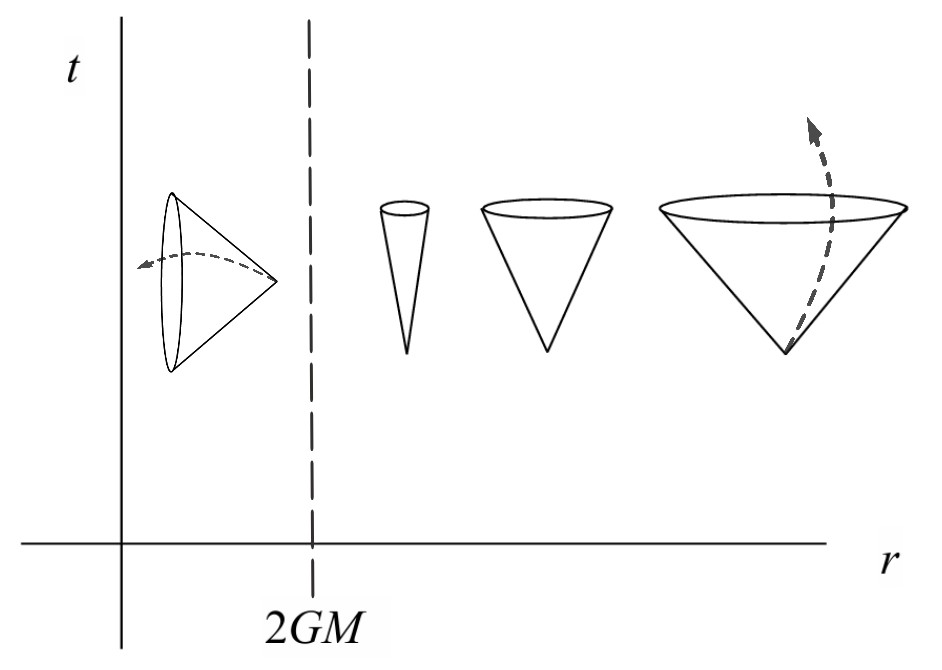
\includegraphics[width=\linewidth]{Figures/Worldlines black hole schwarzschild.jpg}
        \caption{Tilting of light cones in Schwarzschild coordinates. The arrows illustrate possible worldlines of particles.}
        \label{light cones tilted}
    \end{subfigure}
    \hspace{0.5cm}
    \begin{subfigure}[t]{0.46\linewidth}
        \centering
        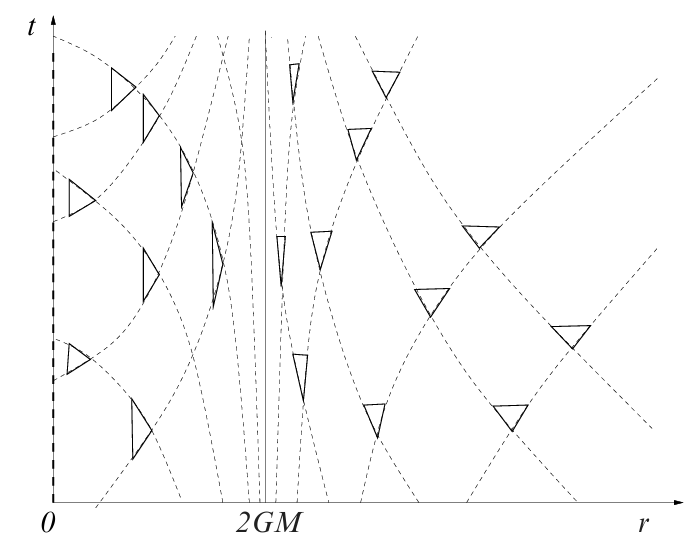
\includegraphics[width=\linewidth]{Figures/2GM.png}
        \caption{Ingoing and outgoing null geodesics in Schwarzschild coordinates.}
        \label{light cones schwarz}
    \end{subfigure}
    \caption{Light cones in the $t-r$ plane of Schwarzschild spacetime. Far from the BH ($r \gg 2GM$), cones open symmetrically at $\pm 45^\circ$, as in flat space. As $r \to 2GM$, the cones progressively close, signaling the presence of the event horizon as a causal boundary. Outside the horizon ($r > 2GM$), the structure resembles Minkowski spacetime. At the horizon ($r=2GM$), the cones degenerate, and inside they invert, pointing inexorably toward the singularity at $r=0$. Original illustrations based on the sources: \cite{LlibreBertJanssen, llibrecarroll2004lectures}.}
    \label{fig:null geodesics}
\end{figure}


Inside the horizon, the situation changes qualitatively. The cones flip orientation and point entirely toward decreasing $r$, forcing all causal trajectories, null and timelike, towards the singularity at $r=0$.

The explicit integration of the null geodesics further clarifies this behavior:
\begin{equation}
t = \pm \left(r + 2GM \ln|r - 2GM| + C_0 \right) ,
\end{equation}
where $C_0$ is an integration constant. The logarithmic term is negligible at large radii but becomes dominant near the horizon. As a result, an outgoing light ray requires an infinite Schwarzschild coordinate time $t$ to reach $r=2GM$, explaining why in these coordinates no signal ever appears to cross the event horizon (see Fig. \ref{light cones schwarz}). 


This leads to an apparent paradox: in Schwarzschild coordinates, no object or signal seems to reach $r=2GM$ as seen by a distant observer. Light from an infalling astronaut, for example, arrives increasingly delayed, redshifted, and fainter, so that from infinity we only ever see them freeze and fade at the horizon. Yet in their own proper time, the crossing occurs in a perfectly finite interval. The issue lies not in the physics but in the coordinates.  


To understand how the interior and exterior regions are connected, and to clarify the causal structure, one needs coordinates that remain regular at $r=2GM$. Standard Schwarzschild coordinates work outside the horizon but break down exactly there, failing to describe geodesics (whether massive or massless) at the surface. The apparent inversion of time and pathological tipping of the light cones signal this inadequacy.  

To follow smoothly the motion of particles or photons across the horizon, one introduces coordinates that treat $r=2GM$ as a coordinate singularity rather than a physical one. A classic choice are the advanced Eddington-Finkelstein coordinates \cite{Eddington--Finkelsteincoordinates}, defined through the transformation
\begin{equation}
    \tilde{t} = t + 2M \log(r - 2M),
\end{equation}
which eliminates the divergence of Schwarzschild time at the horizon.  

In these coordinates, the metric takes the form
\begin{equation}
ds^2 = -\left(1 - \frac{2GM}{r}\right) d\tilde{t}^2 + \frac{4GM}{r}\, d\tilde{t}\,dr + \left(1 + \frac{2GM}{r}\right) dr^2
+ r^2 d\theta^2 + r^2 \sin^2\theta \, d\phi^2 \, ,
\label{exteriorSchwarz}
\end{equation}
which is manifestly regular at $r=2GM$ and allows geodesics, ingoing or outgoing, to be traced continuously across the horizon (see Fig.~\ref{fig:null geodesics}).  

\begin{figure}[h!]
    \centering
    \begin{subfigure}[t]{0.45\linewidth}
        \centering
        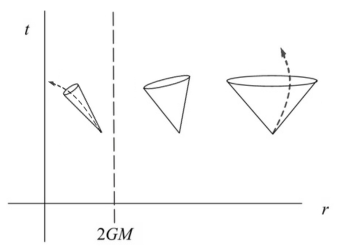
\includegraphics[width=\linewidth]{Figures/Tilting light cones.png}
        \caption{Tilting of light cones in Eddington-Finkelstein coordinates. The arrows illustrate possible worldlines of particles.}
        \label{}
    \end{subfigure}
    \hspace{0.5cm}
    \begin{subfigure}[t]{0.46\linewidth}
        \centering
        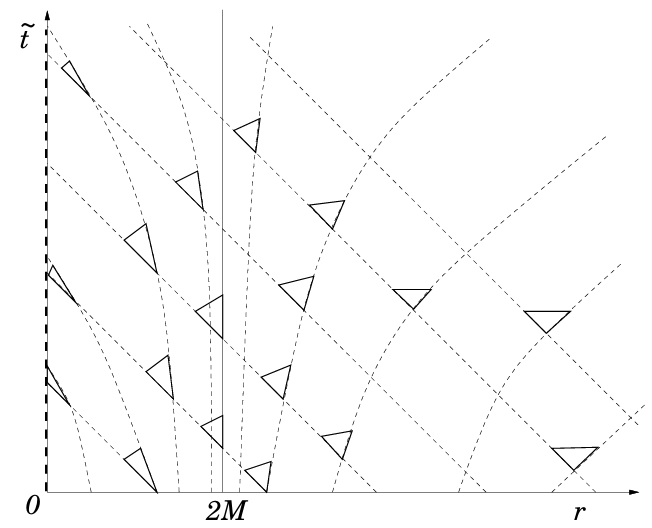
\includegraphics[width=\linewidth]{Figures/Eddington coordinates.png}
        \caption{Ingoing and outgoing null geodesics in Eddington-Finkelstein coordinates.}
        \label{fig:EFK coodinates}
    \end{subfigure}
    \caption{In Eddington-Finkelstein coordinates, the geometry is clarified. For $r \gg 2GM$, light cones resemble those of flat spacetime, opening symmetrically at $\pm 45^\circ$. Closer to the horizon, the cones tip progressively inward. Ingoing null geodesics always remain at $45^\circ$, while outgoing ones tilt more and more as $r \to 2GM$, signaling the increasing difficulty of escaping. At the horizon, the tilt reaches $90^\circ$: an outgoing photon emitted at $r=2GM$ remains trapped. For $r<2GM$, all cones are tipped inward, so even outward-directed light inevitably falls to the singularity. Original illustrations based on the sources: \cite{LlibreBertJanssen, Llibre_Peter_Collier_unacosadificildecomprender}.}
    \label{fig:null geodesics}
\end{figure}


\subsubsection{Black holes in general relativity}

A discussion of GR would be incomplete without addressing BHs. In this section, we have already seen that they naturally emerge from the Schwarzschild solution. We will not delve deeply into their technical details, but we will introduce the essential concepts required to understand, in later sections, the phenomenon of GW. 

BHs are regions of spacetime where gravity is so intense that nothing, not even light, can escape. According to GR, they form when matter becomes sufficiently compressed, curving spacetime to the point that a boundary, called the event horizon, appears (see Fig. \ref{fig:diagram_BH}). This surface acts as a one-way limit: once matter or radiation crosses it, escape is no longer possible. Inside, all trajectories inevitably lead toward a central singularity, where curvature becomes infinite (see Fig. \ref{fig:diagram_BH_complex}).  
\begin{figure}[h!]
    \centering
    \begin{subfigure}[t]{0.3\linewidth}
        \centering
        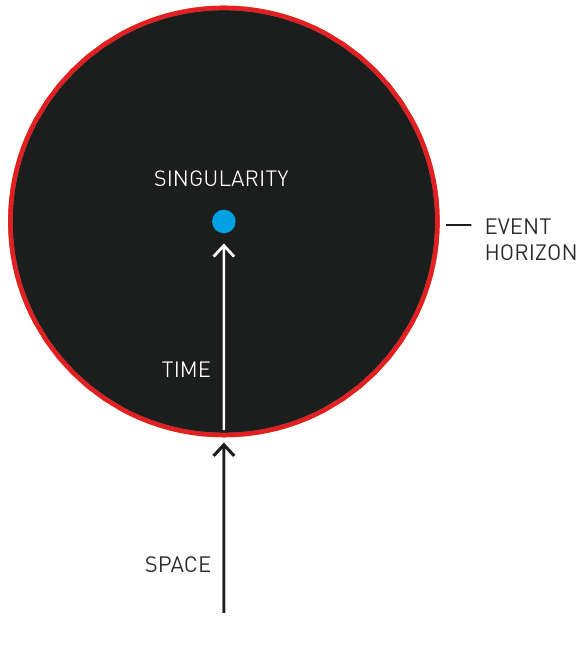
\includegraphics[width=\linewidth]{Figures/diagram_BH_minimalist.png}
        \caption{}
        \label{fig:diagram_BH}
    \end{subfigure}
    \hspace{0.65cm}
    \begin{subfigure}[t]{0.3\linewidth}
        \centering
        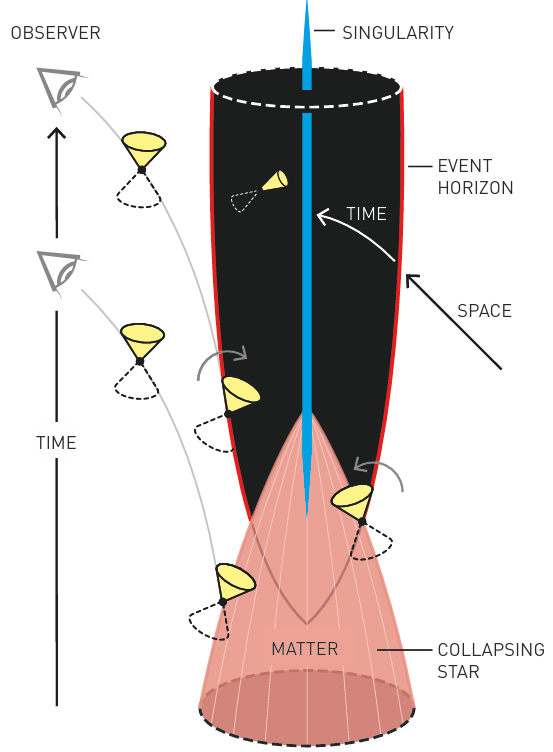
\includegraphics[width=\linewidth]{Figures/diagram_BH_complex.png}
        \caption{}
        \label{fig:diagram_BH_complex}
    \end{subfigure}
    \caption{(a) Simplified depiction of a BH. The event horizon (red line) marks the boundary beyond which nothing can escape. Inside, all paths lead to the singularity (blue dot). (b) More detailed diagram showing the causal structure of a Schwarzschild BH. The light cones tip inward as one approaches the horizon, and inside they point entirely toward the singularity, indicating that all causal trajectories inevitably end there. Source: \cite{nobel2020blackholes}. }
    \label{}
\end{figure}
Although the term BH was popularized by John Wheeler in 1967, the idea traces back to the 18th century, when John Michell and Pierre-Simon Laplace speculated that a star of sufficient density could trap its own light. Their reasoning was based on Newtonian gravity and the notion of escape velocity. While not fully correct, their intuition coincidentally pointed to the same critical radius later derived by Schwarzschild in GR \cite{Llibre_Peter_Collier_unacosadificildecomprender}.  

In nature, BHs most commonly arise from the evolution of massive stars. For stars like the Sun, nuclear fusion generates enough thermal pressure to counterbalance gravity, maintaining equilibrium for billions of years. Once the fuel is exhausted, smaller stars contract into white dwarfs, supported by electron degeneracy pressure. Chandrasekhar showed in 1931 that such stars cannot exceed about 1.4 $M_\odot$; beyond that threshold, gravity overwhelms electron pressure \cite{Llibre_Peter_Collier_unacosadificildecomprender}.  

More massive stars collapse further, producing NSs, stabilized for a time by neutron degeneracy pressure. However, Oppenheimer and collaborators demonstrated that above roughly two to three solar masses, not even this force is sufficient. The star then undergoes unstoppable collapse, crossing its Schwarzschild radius and forming a BH.  

Astrophysical evidence confirms that stellar collapse is not the only mechanism. Observations show the existence of supermassive BHs, with millions to billions of solar masses, at the centers of galaxies, likely formed through accretion and mergers over cosmic time \cite{LlibreBertJanssen}.  


According to the so-called no-hair theorem, BHs are surprisingly simple objects. From the perspective of an outside observer, they can be fully described by only three physical quantities: mass $M$, electric charge $Q$, and angular momentum $J$. This gives rise to four main idealized solutions in GR:  

\begin{itemize}
    \item Schwarzschild BHs, defined only by mass.  
    \item Reissner-Nordström BHs, with mass and electric charge.  
    \item Kerr BHs, with mass and rotation.  
    \item Kerr-Newman BHs, with mass, charge, and rotation.  
\end{itemize}

In practice, astrophysical BHs are expected to be nearly neutral, as any net charge would quickly be neutralized by surrounding plasma. Therefore, the most relevant solutions are Schwarzschild (non-rotating) and Kerr (rotating) BHs. The latter are believed to describe most real BHs, as they likely inherit angular momentum from their progenitor stars or accretion disks.

BHs can also be classified by mass:

\begin{itemize}
    \item \textbf{Stellar-mass black holes (SBHs):} Formed from the collapse of massive stars (typically with $M \gtrsim 20 M_\odot$), they span from a few to hundreds of solar masses. They are often found in binary systems, where they can accrete matter from a companion star and emit X-rays.

    \item \textbf{Intermediate-mass black holes (IMBHs):} These BHs are expected to lie in the mass range $10^2$--$10^5 M_\odot$. While no unambiguous detections exist, several candidates have been suggested from low-luminosity active galactic nuclei, X-ray sources and accretion disk spectra. The strongest evidence comes from GW events: GW190521, the merger of $85^{+21}_{-14} M_\odot$ and $66^{+17}_{-18} M_\odot$ BHs that produced a $142^{+28}_{-16} M_\odot$ remnant \cite{GW190521}, and the more recent GW231123, where BHs of $137^{+22}_{-17} M_\odot$ and $103^{+20}_{-52} M_\odot$ merged into a $225^{+26}_{-43}M_\odot$ remnant \cite{gw231123}.
    \item \textbf{Supermassive black holes (SMBHs):} Located at the centers of galaxies, they range from millions to billions of solar masses. Their origin is still uncertain, but they grow by accretion and mergers. The Milky Way’s central BH, Sagittarius A*, has a mass of about $4 \times 10^6 M_\odot$.
\end{itemize}

In addition to these categories, theorists also propose the existence of primordial black holes (PBHs). These could have formed within the first second after the Big Bang, when extreme densities allowed matter to collapse directly into BHs. Their possible masses are thought to range from as little as $10^{-5}$ grams up to about $10^5 M_\odot$. Quantum effects predict that lighter PBHs would have evaporated over time, but more massive ones could still remain scattered across the universe \cite{nasa_blackholes_types}.

\vspace{0.5cm}

In summary, this chapter has laid the mathematical and physical foundations of GR, progressing from the geometry of curved spacetime and the tools of differential geometry (parallel transport, geodesics, and the Riemann tensor) to the EFE and their most astrophysically relevant solutions: BHs. These concepts constitute the theoretical backbone upon which the remainder of this thesis is built. In the next chapter we turn to the central subject of this work: GWs, which emerge naturally as propagating solutions of the linearized Einstein equations and represent one of the most profound predictions of GR.


\chapter{Gravitational wave theory}
\label{Gravitational-wave theory}

We have now reached the central topic of this thesis and one of the most remarkable predictions of Einstein's GR: GWs. In this chapter, we introduce their theoretical foundations, beginning with their natural emergence from the linearized EFE ($\S$\ref{Gravitational_waves_linearized_gravity}), and characterize their polarization states and physical action on test masses via the geodesic deviation equation. We then survey the main astrophysical source classes ($\S$\ref{Astrophysical_sources_GW}) and discuss the detection principle underlying current interferometric observatories, covering antenna pattern functions, noise sources, and the global detector network ($\S$\ref{}). The chapter closes with an overview of the Bayesian parameter estimation (PE) framework used to extract source properties from GW signals ($\S$\ref{}), establishing the statistical foundation for the data analysis presented in subsequent chapters.

\section{Gravitational waves in linearized gravity}
\label{Gravitational_waves_linearized_gravity}


In 1916, shortly after formulating the final version of his general theory of relativity, Einstein predicted the existence of GWs \cite{Einstein1916GWpaper}. He showed that, within the weak-field or linearized approximation of his equations, spacetime admits wave-like solutions: transverse oscillations of the metric that propagate at the speed of light. These waves are produced by time-dependent variations of the mass quadrupole moment of the source. Einstein also realized that their amplitudes would be extremely small, which led many to doubt their physical reality for decades\footnote{Indeed, until the Chapel Hill conference in 1957 \cite{Chapel_Hill_Conference}, the question of whether GWs were genuine physical phenomena remained under debate .} \cite{GW150914}. 

GWs can be understood as ripples in the curvature of spacetime that carry energy and information about their astrophysical sources. They are generated by asymmetric acceleration of mass or energy, typically in compact binary systems involving BHs (BH-BH), NSs (NS-NS), or mixed BH-NS mergers. The most direct and elegant derivation of their existence arises from the linearized formulation of GR, obtained by expanding the EFE around the flat Minkowski metric $\eta_{\mu\nu}$ \cite{maggiore2007gravitational}.

The first indirect evidence for GWs came from the discovery of the binary pulsar system PSR B1913+16 by Hulse and Taylor in 1974 \cite{Binarypulsar}. Subsequent measurements of its orbital energy loss, provided compelling proof of their existence. This milestone, together with advances in astrophysics, established the foundation for direct GW astronomy \cite{GW150914}.

Nearly a century after Einstein’s prediction, on September 14, 2015, the LIGO Scientific Collaboration (LSC) achieved the first direct detection of GWs, GW150914 \cite{PrimeradeteccioGW150914}, a signal originating from a binary black hole merger (BBH). This event not only confirmed Einstein’s theoretical insight but also inaugurated a new era of observational astrophysics, allowing us to probe relativistic systems in the dynamic, strong-field regime of gravity.


 

\subsection{Linearized gravity}

GR describes gravity as the manifestation of spacetime curvature.
The dynamics of the gravitational field are governed by EFE \cite{maggiore2007gravitational},
\begin{equation}
G_{\mu\nu} \equiv R_{\mu\nu} - \frac{1}{2} g_{\mu\nu} R = 8\pi G \, T_{\mu\nu},
\label{eq:einsteinfieldeqs}
\end{equation}
where $R_{\mu\nu}$ is the Ricci tensor, $R$ the Ricci scalar, and $T_{\mu\nu}$ the
energy-momentum tensor.

The curvature of spacetime is encoded in the Riemann tensor, which is constructed
from the Christoffel symbols. For a torsion free connection, the Christoffel symbols
are defined as \cite{LlibreBertJanssen}
\begin{equation}
\Gamma^\rho_{\mu\nu}
=
\frac{1}{2} g^{\rho\lambda}
\left(
\partial_\mu g_{\lambda\nu}
+
\partial_\nu g_{\lambda\mu}
-
\partial_\lambda g_{\mu\nu}
\right).
\label{eq:christoffelsymbols}
\end{equation}
In terms of these quantities, the components of the Riemann curvature tensor are
given by
\begin{equation}
R^\lambda{}_{\rho\mu\nu}
=
\partial_\mu \Gamma^\lambda_{\rho\nu}
-
\partial_\nu \Gamma^\lambda_{\rho\mu}
+
\Gamma^\lambda_{\sigma\mu}\Gamma^\sigma_{\rho\nu}
-
\Gamma^\lambda_{\sigma\nu}\Gamma^\sigma_{\rho\mu}.
\label{eq:riemanntensor}
\end{equation}
The Riemann tensor fully characterizes the intrinsic curvature of spacetime and
vanishes identically in flat manifolds. By contracting its indices, one obtains the
Ricci tensor \cite{Llibre_Peter_Collier_unacosadificildecomprender},
\begin{equation}
R_{\mu\nu}
=
R^{\rho}{}_{\mu\rho\nu},
\end{equation}
and the Ricci scalar,
\begin{equation}
R
=
g^{\mu\nu} R_{\mu\nu},
\end{equation}
which together determine the Einstein tensor appearing in the field equations.
These geometric quantities provide the starting point for the linearized
description of gravity developed in the following sections.



\subsection{The weak field limit}



As a first step toward the understanding of GWs, we wish to study the expansion of the Einstein equations around the flat space metric in the so called weak field limit. Mathematically, we can write this as
\begin{equation}
g_{\mu\nu} \approx n_{\mu\nu} + h_{\mu\nu}, \qquad |h_{\mu\nu}| \ll 1,
\end{equation}
where $\eta_{\mu\nu}$ is the flat space Minkowski metric $\eta_{\mu\nu}= (-, +, +, +)$ and $h_{\mu\nu}$ represents a small perturbation \cite{maggiore2007gravitational}.

The assumption that $h_{\mu\nu}$ is small allows us to neglect all terms beyond first order in this quantity. The resulting approximation is known as the linearized theory of gravity, and it leads to
\begin{equation}
    g^{\mu\nu} \approx \eta^{\mu\nu} - h^{\mu\nu} + \mathcal{O}(h^2).
\end{equation}
All index operations from this point onward will be performed using the Minkowski metric $\eta_{\mu\nu}$ instead of the full metric $g_{\mu\nu}$ \cite{llibrecarroll2004lectures}. For instance,
\begin{equation}
    h^{\mu\nu} = \eta^{\mu\rho} \eta^{\nu\sigma} h_{\rho\sigma}.
\end{equation}
Our goal is to determine the equation of motion satisfied by the perturbations $h_{\mu\nu}$, which can be obtained by expanding Einstein’s equations to first order. We begin by considering the Christoffel symbols \eqref{eq:christoffelsymbols}, given by
\begin{equation}
    \Gamma^\rho_{\mu\nu} = \frac{1}{2} g^{\rho\lambda}
    \left( \partial_\mu g_{\nu\lambda} + \partial_\nu g_{\mu\lambda} - \partial_\lambda g_{\mu\nu} \right)
    \approx \frac{1}{2} \eta^{\rho\lambda}
    \left( \partial_\mu h_{\nu\lambda} + \partial_\nu h_{\mu\lambda} - \partial_\lambda h_{\mu\nu} \right).
\end{equation}
Here, $g^{\rho\lambda}$ has been replaced by $\eta^{\rho\lambda}$, since all terms of order higher than $h_{\mu\nu}$ are neglected. Using these connection coefficients, we can compute the Riemann tensor \eqref{eq:riemanntensor} as
\begin{equation}
\begin{aligned}
R^{\rho}{}_{\mu \nu \sigma}
&= \partial_\nu \Gamma^{\rho}_{\mu \sigma}
- \partial_\sigma \Gamma^{\rho}_{\mu \nu}
+ \Gamma^{\delta}_{\mu \sigma} \Gamma^{\rho}_{\delta \nu}
- \Gamma^{\delta}_{\mu \nu} \Gamma^{\rho}_{\delta \sigma} \\
&\approx \partial_\nu \Gamma^{\rho}_{\mu \sigma}
- \partial_\sigma \Gamma^{\rho}_{\mu \nu} + \mathcal{O}(h^2) \\
&\approx \frac{1}{2}\eta^{\rho\lambda}
\left( 
\partial_\mu \partial_\nu h_{\lambda \sigma}
- \partial_\nu \partial_\lambda h_{\mu \sigma}
- \partial_\mu \partial_\sigma h_{\lambda \nu}
+ \partial_\lambda \partial_\sigma h_{\mu \nu}
\right) + \mathcal{O}(h^2).
\end{aligned}
\end{equation}
Since the connection coefficients $\Gamma^{\rho}_{\mu\nu}$ are already first order quantities, the only contributions to the Riemann tensor in the linear approximation come from their derivatives, while the quadratic terms in $\Gamma$ can be safely discarded \cite{llibrecarroll2004lectures}.

From the Riemann tensor derived above, we can obtain the linearized Ricci tensor by contracting the indices $\rho$ and $\nu$:
\begin{equation}
\begin{aligned}
R_{\mu \sigma} &= R^{\rho}{}_{\mu \rho \sigma} \approx \frac{1}{2}\eta^{\rho\lambda}(\partial_\mu \partial_\rho h_{\lambda \sigma}
- \partial_\rho \partial_\lambda h_{\mu \sigma}
- \partial_\mu \partial_\sigma h_{\lambda \rho}
+ \partial_\lambda \partial_\sigma h_{\mu \rho})+ \mathcal{O}(h^2) \\
&= \frac{1}{2} \left(\partial_\mu \partial^{\lambda} h_{\lambda \sigma}
- \partial_{\rho} \partial^{\rho} h_{\mu \sigma} 
- \partial_{\mu} \partial_{\sigma} h^{\rho}{}_{\rho}
+ \partial^{\rho} \partial_{\sigma} h_{\mu \rho} \right)+ \mathcal{O}(h^2) \\
&= \frac{1}{2} \left(\partial_\mu \partial^{\lambda} h_{\lambda \sigma} + \partial^{\rho} \partial_{\sigma} h_{\mu \rho}
- \Box h_{\mu \sigma} 
- \partial_{\mu} \partial_{\sigma} h \right)+ \mathcal{O}(h^2),
\label{linearizedriemann}
\end{aligned}
\end{equation}
where $h\equiv h^{\rho}{}_{\rho}\equiv\eta^{\rho\sigma} h_{\rho\sigma}+\mathcal{O}(h^2)$ is the trace of $h_{\mu\nu}$ and $\Box \equiv \partial_{\rho} \partial^{\rho} \equiv \eta^{\rho\sigma} \partial_{\rho} \partial_{\sigma}$ is the D’Alembertian operator \cite{Llibre_Peter_Collier_unacosadificildecomprender}.  

The Ricci scalar is obtained by contracting the Ricci tensor with $\eta^{\mu\sigma}$: 
\begin{equation}
\begin{aligned}
R &\approx \eta^{\mu\sigma} R_{\mu\sigma} \approx \frac{1}{2} \left(\partial_\mu \partial^{\lambda} h_{\lambda}^{\mu} + \partial^{\rho} \partial_{\sigma} h_{\rho}^{\sigma} - \square h 
- \partial_\mu \partial^{\mu} h 
\right) \\
&= \partial_{\sigma} \partial^{\rho} h^{\sigma}_{\rho} - \Box h = \partial^{\nu} \partial^{\rho} h_{\nu\rho} - \Box h ,
\label{lienarizedricci}
\end{aligned}
\end{equation}
where we have interchanged the dummy indices $(\lambda \leftrightarrow \rho)$ and $(\mu \leftrightarrow \sigma)$ in the first term, and used $h^{\sigma}_{\rho}=\eta^{\sigma \nu}h_{\rho \nu}$ in the final equality.

 Once we have these, using the expressions \eqref{linearizedriemann} and \eqref{lienarizedricci} we can compute the linearization of the  Einstein tensor $G_{\mu \nu}=R_{\mu \nu}-(1/2)\eta_{\mu \nu}R$ for a given source
 $T_{\mu \sigma}$ and obtain the linearized form of the EFE \eqref{eq:einsteinfieldeqs}
\begin{equation}
\frac{1}{2} \left(\partial_\mu \partial^{\lambda} h_{\lambda \sigma} + \partial^{\rho} \partial_{\sigma} h_{\mu \rho}
- \Box h_{\mu \sigma} 
- \partial_{\mu} \partial_{\sigma} h \right) - \frac{1}{2} \eta_{\mu \sigma} \left( \partial^{\nu} \partial^{\rho} h_{\nu\rho} - \Box h \right) = 8\pi G T_{\mu \sigma}.
\end{equation}
Since a weak gravitational field corresponds to small spacetime curvature, we can safely assume the absence of matter sources, setting $T_{\mu \sigma} = 0$ we obtain
\begin{equation}
G_{\mu \sigma} \equiv \partial_\mu \partial^{\lambda} h_{\lambda \sigma} + \partial^{\rho} \partial_{\sigma} h_{\mu \rho}
- \Box h_{\mu \sigma} 
- \partial_{\mu} \partial_{\sigma} h  - \eta_{\mu \sigma} \left(\partial^{\nu} \partial^{\rho} h_{\nu\rho} - \Box h \right) = 0.
\end{equation}
To simplify this expression, we introduce the trace reversed perturbation \cite{maggiore2007gravitational}, defined as
 \begin{equation}
    \bar{h}_{\mu\nu} \equiv h_{\mu\nu} - \frac{1}{2}\eta_{\mu\nu}h.
    \label{trace_reversed_perturbation}
 \end{equation}
Observe that the trace of the perturbation satisfies $\bar{h} \equiv \eta^{\mu\nu}\bar{h}_{\mu\nu} = h - 2h = -h$, which allows us to invert the definition in \eqref{trace_reversed_perturbation} to obtain
\begin{equation}
    h_{\mu\nu} = \bar{h}_{\mu\nu} - \frac{1}{2}\eta_{\mu\nu}\bar{h}. 
\end{equation}
Using this relation, we can now express the Einstein tensor entirely in terms of the trace reversed perturbation:
\begin{equation}
\begin{aligned}
G_{\mu\sigma}
&\equiv
\partial_\mu \partial^{\lambda} 
\!\left( \bar{h}_{\lambda\sigma} - \tfrac{1}{2}\eta_{\lambda\sigma}\bar{h} \right)
+ \partial^{\rho} \partial_{\sigma}
\!\left( \bar{h}_{\mu\rho} - \tfrac{1}{2}\eta_{\mu\rho}\bar{h} \right)
- \Box\!\left( \bar{h}_{\mu\sigma} - \tfrac{1}{2}\eta_{\mu\sigma}\bar{h} \right) - \partial_\mu \partial_\sigma(-\bar{h}) \\
&- \eta_{\mu\sigma} \left[
\partial^{\nu}\partial^{\rho}
\!\left( \bar{h}_{\nu\rho} - \tfrac{1}{2}\eta_{\nu\rho}\bar{h} \right)
- \Box(-\bar{h})
\right] = \partial_\mu \partial^{\lambda}\bar{h}_{\lambda\sigma}
- \tfrac{1}{2}\partial_\mu \partial_\sigma \bar{h}
+ \partial^{\rho}\partial_{\sigma}\bar{h}_{\mu\rho} \\
&- \tfrac{1}{2}\partial_\sigma \partial_\mu \bar{h} - \Box \bar{h}_{\mu\sigma} + \tfrac{1}{2}\eta_{\mu\sigma}\Box\bar{h}
+ \partial_\mu \partial_\sigma \bar{h} 
- \eta_{\mu\sigma}\!\left(
\partial^{\nu}\partial^{\rho}\bar{h}_{\nu\rho}
- \tfrac{1}{2}\Box\bar{h}
+ \Box\bar{h} \right).
\end{aligned}
\end{equation}
Finally, by collecting and simplifying all terms, we obtain the compact linearized form of the EFE in vacuum, written in terms of the trace reversed perturbation $\bar{h}_{\mu\nu}$:
\begin{equation}
G_{\mu\sigma} \equiv
\partial_\mu\partial^{\lambda}\bar{h}_{\lambda\sigma}
+ \partial^{\rho}\partial_{\sigma}\bar{h}_{\mu\rho}
- \Box \bar{h}_{\mu\sigma}
- \eta_{\mu\sigma}\partial^{\nu}\partial^{\rho}\bar{h}_{\nu\rho}
= 0.
\label{linearizedEFE}
\end{equation}

\subsubsection{Gauge freedom and the Lorenz condition}

With the linearized field equations at hand, the next step is to address the issue of gauge freedom.  
In GR, the theory remains covariant under arbitrary coordinate transformations.  
This means that even when we decompose the metric as a small perturbation around flat spacetime $g_{\mu\nu} = \eta_{\mu\nu} + h_{\mu\nu}$, the choice of coordinates is not unique. There can exist other coordinate systems in which the metric
can still be expressed as the Minkowski background plus a small perturbation, but with a different
$h_{\mu\nu}$. Hence, this decomposition is not unique \cite{llibrecarroll2004lectures}.

In the linear approximation, an infinitesimal coordinate transformation
\begin{equation}
    x^{\mu} \rightarrow x'^{\mu} = x^{\mu} + \xi^{\mu}(x),
\label{transformation}
\end{equation}
induces a transformation of the perturbation tensor given by
\begin{equation}
    h'_{\mu\nu} = h_{\mu\nu} - \partial_{\mu}\xi_{\nu} - \partial_{\nu}\xi_{\mu},
\end{equation}
where the derivatives $|\partial_{\mu}\xi_{\nu}|$ are taken to be of the same
perturbative order as the metric perturbations $h_{\mu\nu}$.

To simplify the equations, we use the trace reversed perturbation \eqref{trace_reversed_perturbation} \cite{maggiore2007gravitational}:
\begin{equation}
    \bar{h}'_{\mu\nu} = \bar{h}_{\mu\nu}
    - \partial_{\mu}\xi_{\nu}
    - \partial_{\nu}\xi_{\mu}
    + \eta_{\mu\nu}\partial_{\rho}\xi^{\rho}.
\end{equation}
Taking the divergence of this expression leads to
\begin{equation}
    \partial^{\nu}\bar{h}'_{\mu\nu}
    = \partial^{\nu}\bar{h}_{\mu\nu}
    - \Box \xi_{\mu}.
\label{gaugefreedom}
\end{equation}  
We can now exploit the coordinate freedom by choosing the vector $\xi^{\mu}$ to satisfy
\begin{equation}
    \Box \xi^{\mu} = \partial^{\nu}\bar{h}_{\mu\nu}.
\end{equation}
With this choice, the transformed perturbation fulfills
\begin{equation}
    \partial^{\nu}\bar{h}'_{\mu\nu} = 0,
\label{lorenzgauge}
\end{equation}
which defines the Lorenz gauge condition \cite{maggiore2007gravitational} (also called the harmonic gauge or the De Donder gauge):
\begin{equation}
    \partial^{\nu}\bar{h}_{\mu\nu} = 0.
\label{Lorenz_gauge_condition}
\end{equation}
Imposing the Lorenz condition simplifies the linearized Einstein equations \eqref{linearizedEFE} to
\begin{equation}
    \Box \bar{h}_{\mu\nu} = 0,
\label{linearized_wave_equation}
\end{equation}
which is the standard wave equation in flat spacetime. 

\subsubsection{Solving the wave equation and the Transverse-Traceless gauge}

We are now interested in solving the linearized equation \eqref{linearized_wave_equation} to find the form of GWs. The general solution of the linearized wave equation can be written as a superposition of plane waves:
\begin{equation}
    \bar{h}_{\mu\nu}(x) = \text{Re} \left\{ A_{\mu\nu} e^{i k_\alpha x^\alpha} \right\},
\label{waveequation}
\end{equation}
where $A_{\mu\nu}$ is a complex, symmetric polarization tensor and $k_\alpha$ is the wave four-vector \cite{llibreRamosSanchez2018}. 

Substituting this ansatz into the wave equation \eqref{linearized_wave_equation}, we obtain 
\begin{equation}
    k^\sigma k_\sigma = 0.
\end{equation}
This implies that, for non-trivial solutions $\bar{h}_{\mu\nu} \neq 0$, the wave four-vector must be null. That is, the perturbations propagate at the speed of light\footnote{A null wave four-vector satisfies $k^\mu k_\mu = 0$, which in Minkowski spacetime reads $\omega^2 - |\mathbf{k}|^2 = 0$. 
This relation implies $\omega = |\mathbf{k}|$, so the phase velocity of the perturbation is $v = \omega / |\mathbf{k}| = c$. 
Therefore, GWs correspond to massless excitations of the gravitational field that propagate at the speed of light in vacuum \cite{llibretongGR}.} (GWs in vacuum) \cite{llibrecarroll2004lectures}.


Furthermore, applying the Lorenz gauge condition \eqref{Lorenz_gauge_condition} to the wave equation \eqref{waveequation}, we can prove that:
\begin{equation}
A_{\mu\nu} k^\mu = 0,
\end{equation}
which shows that GWs are transverse with respect to their direction of propagation.

After applying the Lorenz gauge condition \eqref{lorenzgauge}, there still remains a residual gauge freedom that allows further simplification. This residual freedom is a consequence of the fact that the Lorenz gauge does not completely eliminate coordinate freedom. As follows from \eqref{gaugefreedom}, under the transformation
\eqref{transformation} the quantity $\partial^\nu \bar{h}_{\mu\nu}$ transforms
homogeneously. As a result, the gauge condition
$\partial^\nu \bar{h}_{\mu\nu} = 0$ remains invariant under additional coordinate
transformations of the form $x^\mu \rightarrow x^\mu + \xi^\mu$, provided that
the vector field $\xi^\mu$ satisfies
\begin{equation}
\Box \xi^\mu = 0.
\end{equation}
If $\Box \xi^\mu = 0$, then the symmetric tensor
\begin{equation}
\xi_{\mu\nu} = \partial_\mu \xi_\nu + \partial_\nu \xi_\mu - \eta_{\mu\nu}
\partial_\rho \xi^\rho ,
\end{equation}
also fulfills $\Box \xi_{\mu\nu} = 0$, since the flat d’Alembertian operator
commutes with partial derivatives. Consequently, solutions of the wave equation
for $\bar{h}_{\mu\nu}$ remain invariant under the subtraction of such terms.

This residual gauge freedom allows one to impose four additional conditions on
$h_{\mu\nu}$. In particular, one may choose the gauge such that the trace
vanishes, $h = 0$, implying $\bar{h}_{\mu\nu} = h_{\mu\nu}$. Furthermore, the
remaining gauge freedom can be used to set $h_{0\mu} = 0$. The Lorenz condition
then reduces to
\begin{equation}
\partial^j h_{ij} = 0,
\end{equation}
while the traceless condition becomes $h^i{}_i = 0$.

In summary, we can impose the conditions
\begin{equation}
h_{0\mu} = 0, \qquad h^i{}_i = 0, \qquad \partial^j h_{ij} = 0,
\end{equation}
which define the transverse-traceless (TT) gauge \cite{maggiore2007gravitational}. The first condition indicates that GWs possess only spatial components (since the symmetry enforces $h_{\mu 0} = h_{0 \mu} = 0$). The second condition implies that the perturbation is traceless, meaning the sum of the diagonal elements of the perturbation matrix vanishes. Finally, the last relation reveals that the perturbation is transverse, such that the amplitude tensor is orthogonal to the direction of propagation.

As a result, the degrees of freedom of $A_{\mu\nu}$ are reduced from ten to only two independent components, indicating that a GW has only two physical degrees of freedom, corresponding to its two polarization states \cite{llibreFerrariValeriaGR}.  

An important feature of working in the TT gauge is that the vanishing trace condition implies
\begin{equation}
    \bar{h}_{\mu\nu} = h_{\mu\nu}.
\end{equation}
Therefore, the plane wave solution can be expressed as
\begin{equation}
    h_{\mu\nu}^{\text{TT}} = A_{\mu\nu} e^{i k_\alpha x^\alpha},
\end{equation}
where $h_{\mu\nu}^{\text{TT}}$ represents the metric perturbation in the TT gauge.


\subsection{Polarization states}

Considering a wave propagating in the $z$-direction, we can choose the wave four-vector as $k^\mu = (\omega/c, 0, 0, \omega/c)$. The Lorenz gauge \eqref{Lorenz_gauge_condition} implies $A_{\mu 0} + A_{\mu 3} = 0$\footnote{If the gauge condition requires $h_{\mu 0}=0$ for all spacetime points and the metric perturbation is written as 
$h_{\mu\nu}=A_{\mu\nu}e^{i k_\rho x^\rho}$, the exponential factor never vanishes. 
Therefore, the only way for $h_{\mu 0}$ to be identically zero is that the corresponding amplitude components vanish $A_{\mu 0}=0$ (and, by symmetry, $A_{0\mu}=0$) \cite{llibretongGR}.} and the additional TT gauge conditions lead to $A_{\mu 0} = 0$.  
Thus, the only non-zero components of the amplitude tensor are $A_{11}$, $A_{22}$, and $A_{12} = A_{21}$. The traceless condition $A^{i}{}_{i} = 0$ further implies that $A_{11} + A_{22} = 0$, allowing us to express the TT perturbation as
\begin{equation}
h^{TT}_{\mu\nu}\, (t,z) =
\begin{pmatrix}
0 & 0 & 0 & 0 \\
0 & h^{TT}_{+} & h^{TT}_{\times} & 0 \\
0 & h^{TT}_{\times} & -h^{TT}_{+} & 0 \\
0 & 0 & 0 & 0
\end{pmatrix}_{\mu\nu}
=
\begin{pmatrix}
0 & 0 & 0 & 0 \\
0 & A_{+} & A_{\times} & 0 \\
0 & A_{\times} & -A_{+} & 0 \\
0 & 0 & 0 & 0
\end{pmatrix}_{\mu\nu}
e^{-i\omega (t - z / c)} ,
\end{equation}
where $h^{TT}_{+}$ and $h^{TT}_{\times}$ represent the two independent and orthogonal polarization states of the GW, commonly referred to as the plus and cross modes \cite{llibretongGR}. Returning from the complex to the real domain, the strain can finally be expressed as
\begin{equation}
h^{TT}_{\mu\nu}\, (t,z) =
\begin{pmatrix}
0 & 0 & 0 & 0 \\
0 & A_{+} & A_{\times} & 0 \\
0 & A_{\times} & -A_{+} & 0 \\
0 & 0 & 0 & 0
\end{pmatrix}_{\mu\nu}
\cos \, [\, \omega \, (t - z / c)], 
\label{polarizationmodes}
\end{equation}
where $A_{+}$ and $A_{\times}$ denote the amplitudes of the two polarization modes.



\subsection{Effect of a gravitational wave on test masses}
\label{geodesic_eq_sec}

In order to describe the physical influence of a GW on a given
system, we analyze the motion of test particles in its presence. A
coordinate independent characterization of this effect is provided by the
relative motion of nearby particles. This behavior is governed by the geodesic
deviation equation \cite{llibrecarroll2004lectures}, which captures how a GW modifies the
separation between neighboring geodesics
\begin{equation}
a^\mu
= \frac{D^2 S^\mu}{d t^2}
= R^\mu{}_{\nu\rho\sigma} \, U^\nu U^\rho S^\sigma ,
\label{geodesicdeviation}
\end{equation}
where $S^\mu$ denotes the separation between two neighboring geodesics, $U^\mu = dx^\mu / dt$ is the tangent vector to the reference geodesic,  $a^\mu$ represents the relative acceleration between the two test particles and $R^\mu{}_{\nu\rho\sigma}$ is the Riemann curvature tensor,


Before analyzing the effect of a GW on an extended system of
test masses, it is instructive to examine its influence on a single particle.
We consider a particle initially at rest in flat spacetime, prior to the
arrival of the wave. An inertial reference frame is attached to this particle,
with the $x$-axis chosen along the direction of propagation of an incoming
TT GW. The particle subsequently follows
a geodesic of the perturbed spacetime generated by the wave.

The motion of the particle is governed by the geodesic equation,
\begin{equation}
\frac{d^2 x^\alpha}{d\tau^2}
+ \Gamma^\alpha_{\mu\nu}
\frac{d x^\mu}{d\tau}
\frac{d x^\nu}{d\tau}
=
\frac{d U^\alpha}{d\tau}
+ \Gamma^\alpha_{\mu\nu} U^\mu U^\nu
= 0 .
\end{equation}

At $\tau = 0$, the particle is at rest in this frame, so that
$U^\alpha = (1,0,0,0)+ \mathcal{O}(h)$. The acceleration induced by the GW at
this instant is therefore given by
\begin{equation}
\left. \frac{d U^\alpha}{d\tau} \right|_{\tau=0}
=
- \Gamma^\alpha_{00}
=
- \frac{1}{2} \eta^{\alpha\beta}
\left(
h_{\beta 0 , 0}
+ h_{0 \beta , 0}
- h_{00 , \beta}
\right).
\end{equation}
However, in the TT gauge all components $h_{0\mu}$ vanish.
As a consequence,
\begin{equation}
\left. \frac{d U^\alpha}{d\tau} \right|_{\tau=0} = 0 .
\end{equation}
The four-velocity thus remains constant at all times, implying that the
particle experiences no coordinate acceleration due to the passage of the
GW. Its coordinate position therefore remains unchanged. This result shows that the motion of a single freely falling particle is
insufficient to reveal the presence of a GW. Detectable effects
arise only when considering the relative motion between multiple nearby test
masses \cite{llibreFerrariValeriaGR}.


Having established that the motion of a single freely falling particle does not provide a direct observable signature of a GW, we now turn to the physically relevant case of a system of test particles. Observable effects arise from the relative motion between nearby particles, which is invariant under coordinate transformations.

We consider a congruence of neighbouring timelike geodesics describing freely falling test particles. In the absence of gravitational radiation, these particles are initially at rest with respect to a common inertial frame, so that their four-velocity is
\begin{equation}
U^\mu = (1,0,0,0)+ \mathcal{O}(h).
\end{equation}
At some reference time $t=0$, a plane GW propagating along the $z$-direction passes through the system. We work throughout in the TT gauge, where the only non vanishing components of the metric perturbation lie in the plane orthogonal to the direction of propagation.

The relative motion of neighbouring particles is governed by the geodesic deviation equation \eqref{geodesicdeviation}. In the linearised regime of gravity, the Riemann tensor is already first order in the metric perturbation $h_{\mu\nu}$. Consequently, it is sufficient to evaluate the equation using the unperturbed four-velocity $U^\mu = (1,0,0,0)$, and to identify the coordinate time $t$ with the proper time along the geodesics, up to corrections of order $\mathcal{O}(h^2)$.

Using the alredy computed expression for the linearised Riemann tensor in the TT gauge, 
\begin{equation}
\begin{aligned}
R^{\rho}{}_{\mu \nu \sigma}
&= \frac{1}{2}\eta^{\rho\lambda}
\left( 
\partial_\mu \partial_\nu h_{\lambda \sigma}
- \partial_\nu \partial_\lambda h_{\mu \sigma}
- \partial_\mu \partial_\sigma h_{\lambda \nu}
+ \partial_\lambda \partial_\sigma h_{\mu \nu}
\right) + \mathcal{O}(h^2),
\end{aligned}
\end{equation}
one finds that the only non vanishing components relevant for the geodesic deviation equation are
\begin{equation}
R^i{}_{0 0 j} =\frac{1}{2}\eta^{\rho\lambda}
\left( 
\partial_0 \partial_0 h_{\lambda \sigma}
- \partial_0 \partial_\lambda h_{0 \sigma}
- \partial_0 \partial_\sigma h_{\lambda 0}
+ \partial_\lambda \partial_\sigma h_{0 0}
\right) + \mathcal{O}(h^2)= \frac{1}{2}\,\partial_t^2 h_{ij}+ \mathcal{O}(h^2),
\end{equation}
where $i,j = 1,2,3$ label spatial coordinates. The equation of motion for the spatial components of the separation vector then reduces to
\begin{equation}
\frac{d^2 S^i}{dt^2} = \frac{1}{2}\,\partial_t^2 h^{TT}_{ij}\, S^j.
\label{eq:geodesiceq}
\end{equation}
This result shows explicitly that the GW induces tidal forces only in the plane transverse to the direction of propagation. For a wave travelling along the $z$-axis, the longitudinal component $S^3$ remains unaffected, while the transverse components $(S^1,S^2)$ encode the physical deformation of the system.


Integrating the equation we find
\begin{equation}
S^i(t) = S^i(0) + \frac{1}{2}\, h^{TT}_{ij}(t)\, S^j(0).
\label{solutioneqdeviation}
\end{equation}
For a general superposition of the two polarizations, the metric perturbation in
the TT gauge can be written as
\begin{equation}
h^{TT}_{ij}(t,z) =
\begin{pmatrix}
A_{+} & A_{\times} & 0 \\
A_{\times} & -A_{+} & 0 \\
0 & 0 & 0
\end{pmatrix}_{ij}
\, e^{-i \omega (t - z / c)} .
\end{equation}
Restricting to the spatial components and inserting this expression into the
solution of the geodesic deviation equation \eqref{solutioneqdeviation}, one obtains
\begin{equation}
\begin{aligned}
S^x(t) &=
\left(1 + \frac{1}{2} A_{+} e^{-i \omega (t - z / c)} \right) S^x(0)
+ \frac{1}{2} A_{\times} e^{-i \omega (t - z / c)} \, S^y(0), \\[6pt]
S^y(t) &=
\left(1 - \frac{1}{2} A_{+} e^{-i \omega (t - z / c)} \right) S^y(0)
+ \frac{1}{2} A_{\times} e^{-i \omega (t - z / c)} \, S^x(0), \\[6pt]
S^z(t) &= S^z(0),
\end{aligned}
\end{equation}
which are coupled equations for the transverse components of the separation vector.

Since the geodesic deviation equation is linear in the metric perturbation
$h^{TT}_{\mu\nu}$, the response of the system to a GW is also
linear. As a consequence, the effects produced by a general superposition of the
two independent polarizations can be obtained as the sum of the responses to
each polarization separately. It is therefore sufficient to analyze the cases
of purely $+$ and purely $\times$ polarized waves independently, without loss
of generality \cite{llibretongGR}.


If the cross polarization vanishes, $A_{\times}=0$, the metric perturbation
reduces to
\begin{equation}
h^{TT}_{ij}(t,z) =
\begin{pmatrix}
A_{+} & 0 & 0 \\
0 & -A_{+} & 0 \\
0 & 0 & 0
\end{pmatrix}_{ij}
\, e^{-i \omega (t - z / c)} .
\end{equation}
The corresponding evolution of the separation vector is then
\begin{equation}
\begin{aligned}
S^x(t) &=
\left(1 + \frac{1}{2} A_{+} e^{-i \omega (t - z / c)} \right) S^x(0), \\[6pt]
S^y(t) &=
\left(1 - \frac{1}{2} A_{+} e^{-i \omega (t - z / c)} \right) S^y(0), \\[6pt]
S^z(t) &= S^z(0),
\end{aligned}
\end{equation}
where as mentioned in \eqref{polarizationmodes}, we should take the real part of the exponential. This polarization produces an oscillatory stretching and squeezing of the particle distribution along the transverse axes (see Fig.  \ref{fig:geodesic_comparison}).


If the plus polarization vanishes, $A_{+}=0$, the metric perturbation becomes
\begin{equation}
h^{TT}_{ij}(t,z) =
\begin{pmatrix}
0 & A_{\times} & 0 \\
A_{\times} & 0 & 0 \\
0 & 0 & 0
\end{pmatrix}_{ij}
\, e^{-i \omega (t - z / c)} .
\end{equation}

In this case, the solution of the geodesic deviation equation reads
\begin{equation}
\begin{aligned}
S^x(t) &= S^x(0)
+ \frac{1}{2} A_{\times} e^{-i \omega (t - z / c)} \, S^y(0), \\[6pt]
S^y(t) &= S^y(0)
+ \frac{1}{2} A_{\times} e^{-i \omega (t - z / c)} \, S^x(0), \\[6pt]
S^z(t) &= S^z(0).
\end{aligned}
\end{equation}

This polarization induces a shear deformation in the transverse plane, with
principal axes rotated by $45^\circ$ with respect to the $x$ and $y$ directions (see Fig. \ref{fig:geodesic_comparison}).



\begin{figure}[h!]
    \centering
    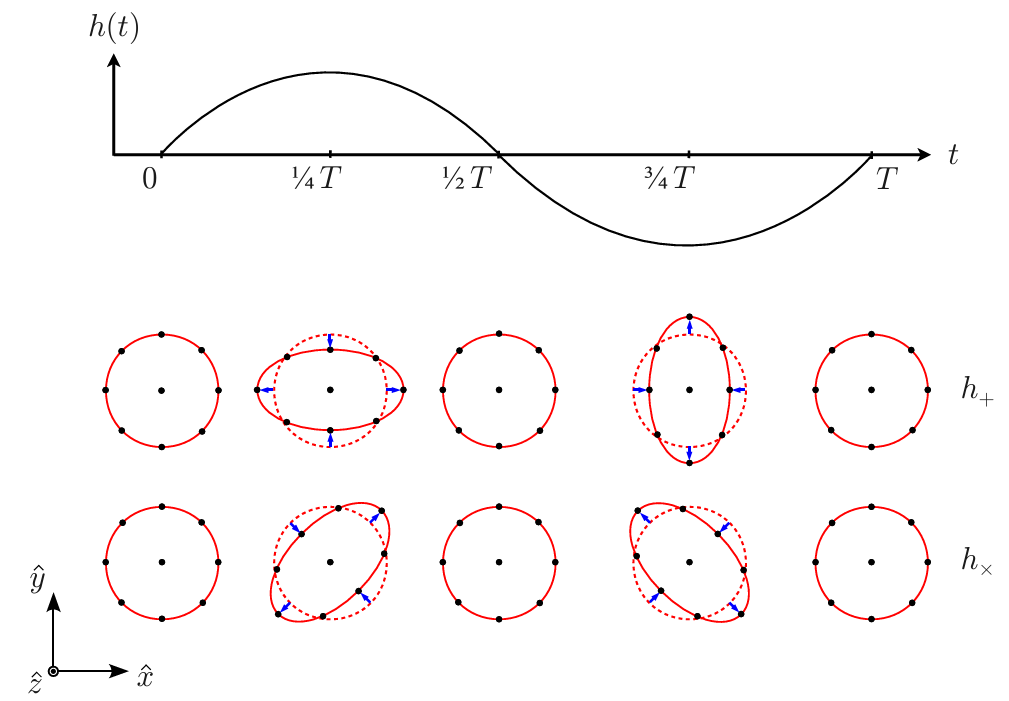
\includegraphics[width=0.71\linewidth]{Figures/Captura de pantalla 2025-12-30 180922.png}
    \caption{A monochromatic GW with angular frequency $\omega = 2\pi/T$ propagates in the $\hat{z}$ direction. The lower panel illustrates the deformation produced by the $+$ and $\times$ polarization modes on a ring of freely falling test particles in a local inertial frame. Source: \cite{Theory_of_Gravitational_Waves_arxiv}.}
    \label{fig:geodesic_comparison}
\end{figure}


\subsection{Generation of gravitational waves}

In the previous sections we described GWs as propagating perturbations of the space-time metric and analyzed their effect on matter. We now turn to the inverse question: how dynamical matter sources generate gravitational radiation.

A conceptual subtlety immediately appears. GW emission can take place in strongly non-linear regimes, such as the late stages of CBCs, where the full Einstein equations are required to describe the dynamics near the source. However, the radiation detected far from the source is typically very weak, so that the metric can be written as a small perturbation of flat space-time. This justifies studying GW generation in the local wave zone within the framework of linearized gravity (see Fig. \ref{fig:zones}).
\begin{figure}[h!]
    \centering
    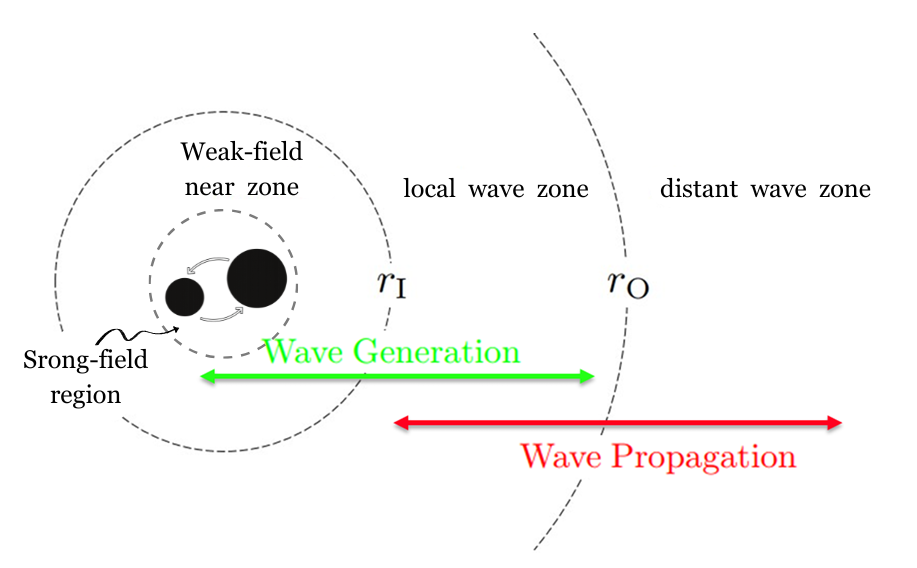
\includegraphics[width=0.66\linewidth]{Figures/near zone.png}
    \caption{Spatial regions associated with a compact binary source of GWs. The strong-field region, weak-field near zone, and the local and distant wave zones are indicated, separated by the characteristic scales $r_I$ and $r_O$. GW generation predominantly occurs in the near zone (green arrow), while wave propagation is described in the distant wave zone (red arrow). Original illustration based on the sources: \cite{zonesofinfluence, thorne2009lorentz}.}
    \label{fig:zones}
\end{figure}

We therefore consider the linearized Einstein equations in the presence of matter, assuming weak gravitational fields and slowly moving sources, so that the background metric can be approximated as Minkowski and internal velocities are small compared to the speed of light. Under these conditions the problem becomes analytically tractable and closely analogous to electromagnetic radiation from accelerated charges \cite{Theory_of_Gravitational_Waves_arxiv}.

In contrast with electromagnetism, conservation laws strongly constrain gravitational radiation. Mass conservation excludes monopole radiation, while conservation of linear and angular momentum eliminates dipole contributions. Consequently, the leading radiative term arises from the time variation of the mass quadrupole moment of the source.


\subsubsection{Einstein's quadrupole formula}
\label{quadrupole_sec}

The starting point is the linearized Einstein equation \eqref{linearized_wave_equation} in the presence of matter, written in harmonic gauge,
\begin{equation}
\square \bar{h}_{\mu\nu} = - \frac{16\pi G}{c^4} T_{\mu\nu},
\end{equation}
where $\bar h_{\mu\nu} = h_{\mu\nu} - \tfrac{1}{2}\eta_{\mu\nu} h$ denotes the trace-reversed metric perturbation and $T_{\mu\nu}$ is the energy-momentum tensor of the source (see $\S$\ref{The energy-momentun tensor}). The Lorenz gauge condition $\partial^\mu \bar{h}_{\mu\nu}=0$ is consistent provided that energy-momentum is conserved, $\partial^\mu T_{\mu\nu}=0$.

As in electromagnetism, this set of decoupled wave equations can be solved using Green's function techniques \cite{maggiore2007gravitational}. For an isolated source localized within a finite spatial region $\Sigma$, the retarded solution is
\begin{equation}
\bar{h}_{\mu\nu}(t,\mathbf{x}) = \frac{4G}{c^4} 
\int_{\Sigma} \frac{T_{\mu\nu}(t_{\rm ret},\mathbf{x}')}{|\mathbf{x}-\mathbf{x}'|} \, d^3x',
\end{equation}
where the retarded time is
\begin{equation}
t_{\rm ret} = t - \frac{|\mathbf{x}-\mathbf{x}'|}{c}.
\end{equation}
This expression explicitly enforces causality: the metric perturbation at $(t,\mathbf{x})$ depends on the configuration of the source at the earlier time $t_{\rm ret}$ (see Fig. \ref{fig:lightconeGW}) \cite{llibretongGR}.


\begin{figure}[h!]
    \centering
    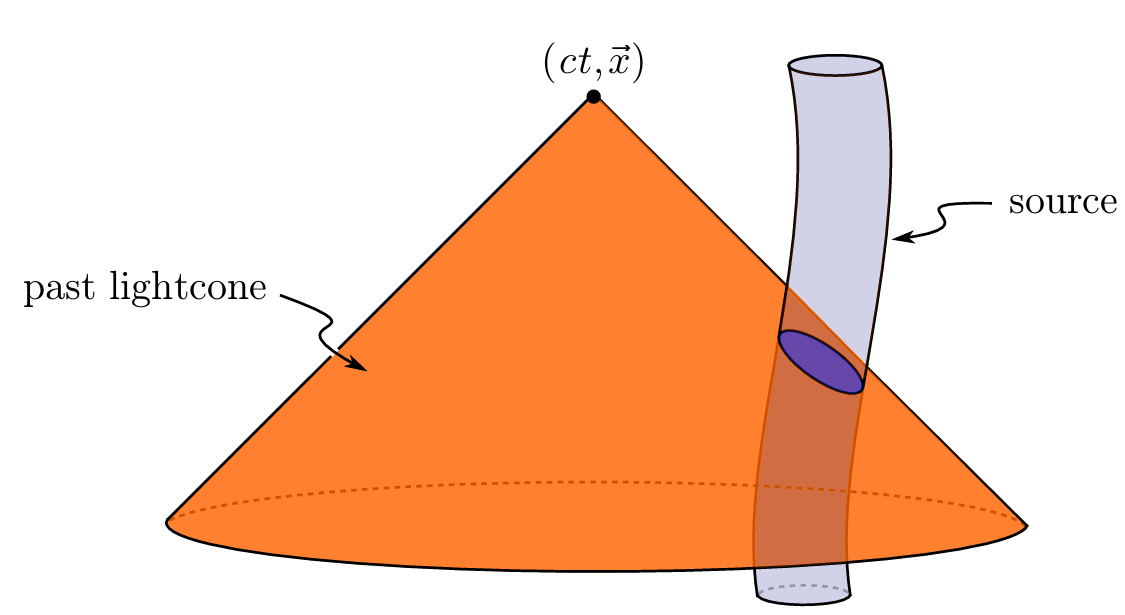
\includegraphics[width=0.64\linewidth]{Figures/lightconeGW.png}
    \caption{Representation of the past light cone of the observation event $(ct,\mathbf{x})$. GWs propagate at the finite speed $c$, so the metric perturbation measured at the detector is determined by the configuration of the source at the retarded time $t' = t - |\mathbf{x}-\mathbf{y}|/c$. Only the portion of the source worldtube intersecting the past light cone contributes to the observed gravitational field, ensuring causal propagation. Source: \cite{Theory_of_Gravitational_Waves_arxiv}.}
    \label{fig:lightconeGW}
\end{figure}

We are interested in the radiation observed far from the source, in the wave zone, where 
$r = |\mathbf{x}|$ is much larger than both the source size $R$ and the gravitational wavelength $\lambda$. 
In this regime one expands
\begin{equation}
\mathbf{x}-\mathbf{x}'| \simeq r - \mathbf{n}\cdot\mathbf{x}',
\qquad
\mathbf{n} = \frac{\mathbf{x}}{r},
\end{equation}
and keeps only the leading terms in $1/r$ and in $v/c$.

Conservation laws severely restrict the possible radiative multipoles. By \href{https://en.wikipedia.org/wiki/Birkhoff%27s_theorem_(relativity)}{Birkhoff’s theorem}, any spherically symmetric mass distribution produces a static exterior solution, so a time-varying monopole term cannot radiate. Furthermore, the first time derivative of the mass dipole moment is proportional to the total linear momentum of the system, which is conserved for an isolated source. As a result, both monopole and dipole radiation are absent in GR.

The leading contribution to gravitational radiation therefore arises at quadrupole order. Keeping the lowest non-vanishing term in the multipole expansion and restricting to non-relativistic sources, one finds that the dominant spatial components of the metric perturbation are
\begin{equation}
\bar h_{ij}(t,\mathbf{x}) = \frac{2G}{c^4 r} \,
\ddot I_{ij}(t - r/c),
\end{equation}
where
\begin{equation}
I_{ij}(t) = \int_{\mathcal{S}} \rho(t,\mathbf{x})\, x_i x_j \, d^3x,
\end{equation}
is the (Newtonian) mass moment of inertia tensor of the source $\mathcal{S}$ and $\rho$ is the (Newtonian) mass density.

At this stage the solution is still written in harmonic gauge and is not yet transverse nor traceless. 
The radiative degrees of freedom are obtained by extracting the TT part of the spatial metric perturbation. 
Outside the source, where $T_{\mu\nu}=0$, this can be done by applying the TT projection operator,
\begin{equation}
h_{ij}^{\rm TT} = \Lambda_{ij,kl}\,\bar h_{kl},
\end{equation}
with
\begin{equation}
\Lambda_{ij,kl} = P_{ik}P_{jl} - \frac{1}{2}P_{ij}P_{kl},
\qquad
P_{ij} = \delta_{ij} - n_i n_j.
\end{equation}
It is convenient to introduce the traceless mass quadrupole moment,
\begin{equation}
\mathcal{I}_{ij}(t)
=
\int \rho(t,\mathbf{x})
\left(
x_i x_j - \frac{1}{3} r^2 \delta_{ij}
\right)
d^3x,
\end{equation}
which differs from $I_{ij}$ only by a trace term. 
Since the TT projection automatically removes traces, one may equivalently replace $I_{ij}$ by $\mathcal{I}_{ij}$ in the radiative formula.

Combining the far-zone expansion with the TT projection, the metric perturbation takes the form
\begin{equation}
h_{ij}^{\rm TT}(t,\mathbf{x})
=
\frac{2G}{c^4 r}
\Lambda_{ij,kl}\,
\ddot{\mathcal{I}}_{kl}(t - r/c).
\end{equation}  

This is Einstein’s quadrupole formula: 
the gravitational radiation measured far from an isolated source 
is proportional to the second time derivative of its traceless mass quadrupole moment, 
evaluated at the retarded time \cite{Theory_of_Gravitational_Waves_arxiv}. In particular, for compact binary systems the symmetry of the quadrupole tensor 
implies that the dominant gravitational radiation oscillates at twice the orbital frequency.

The quadrupole moment formalism provides the leading-order description 
of GW emission from isolated systems. Although originally derived by 
Einstein for non-gravitationally driven sources, it was later shown to 
hold also for self-gravitating systems in the weak-field, Newtonian 
regime. In this limit, the quadrupole moment is computed from the 
Newtonian mass density, and the resulting metric perturbation in the 
TT gauge gives the dominant radiative contribution, with higher-order 
multipoles and relativistic corrections appearing at post-Newtonian order 
\cite{blanchet2024postnewtoniantheorygravitationalwaves}.

\subsubsection{Radiated energy}

A system that radiates GWs necessarily undergoes an energy loss. It is therefore important to quantify the amount of energy carried away by the radiation. In other words, we aim to determine the energy flux transported by GWs away from the source.

The formula for the energy flux of GWs can be derived by considering the effective stress-energy tensor of the gravitational field in the wave zone. In the TT gauge, the energy flux per unit area is given by
\begin{equation}
\frac{dE}{dA dt} = \frac{c^3}{16\pi G} \langle \dot{h}_{ij}^{\rm TT} \dot{h}_{ij}^{\rm TT} \rangle,
\end{equation}
where the angle brackets denote an average over several wavelengths or periods of the wave. This expression shows that the energy flux is proportional to the square of the time derivative of the metric perturbation, reflecting the fact that GWs carry energy away from their sources.
Integrating the energy flux over a sphere of radius $r$ centered on the source, one obtains the total power radiated in GWs,
\begin{equation}
P = \frac{c^3 r^2}{16\pi G} \int \langle \dot{h}_{ij}^{\rm TT} \dot{h}_{ij}^{\rm TT} \rangle d\Omega,
\end{equation}where the integral is taken over the solid angle $\Omega$. Substituting the quadrupole formula for $h_{ij}^{\rm TT}$, one finds the well-known expression for the power radiated by a source with mass quadrupole moment $\mathcal{I}_{ij}$,
\begin{equation}
P = \frac{G}{5c^5} \langle \dddot{\mathcal{I}}_{ij} \dddot{\mathcal{I}}_{ij} \rangle,
\end{equation}
where the triple dot denotes the third time derivative. This formula quantifies the energy loss due to GW emission in terms of the third time derivative of the mass quadrupole moment of the source. For compact binary systems, this energy loss leads to a gradual inspiral of the orbit, which can be observed as a characteristic chirp signal in the GW waveform \cite{maggiore2007gravitational}.



\section{Astrophysical sources}
\label{Astrophysical_sources_GW}

GW astronomy identifies four broad categories of astrophysical signals, each characterized by distinct time-scales, amplitudes, and expected sources. These categories are commonly referred to as transient (compact binary coalescences (CBCs) and bursts), continuous waves (CWs) and stochastic gravitational wave background (SGWB) (see Fig. \ref{fig:sources}) \cite{Astrophysicalsources}.

\begin{figure}[h!]
    \centering
    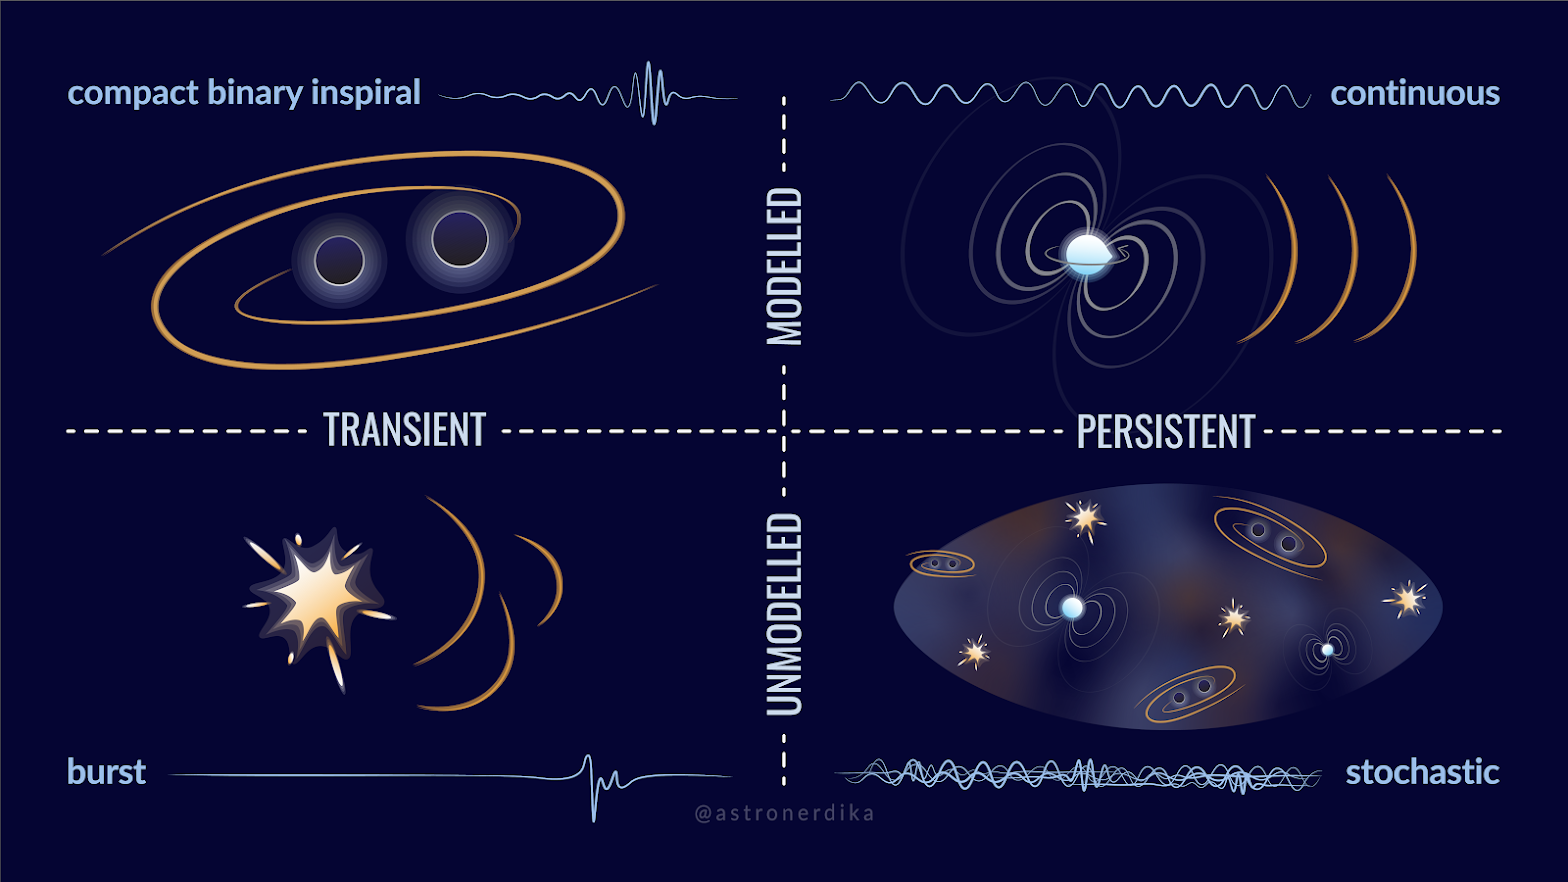
\includegraphics[width=0.69\linewidth]{Figures/GW_types.png}
    \caption{Classification of GW sources according to their temporal character (transient vs.\ persistent) and the availability of accurate waveform models (modelled vs.\ unmodelled), encompassing CBCs, burst events, continuous waves, and the stochastic background. Credit: Shanika Galaudage (@astronerdika).}
    \label{fig:sources}
\end{figure}


\subsection{Compact binary coalescences}  

CBCs are systems formed by two compact objects such as BHs, NSs, or a combination of both, which inspiral and merge due to the emission of GWs (see Fig.~\ref{fig:inspiral_merger_ringdown}). 
\newpage

\begin{figure}[h!]
    \centering
    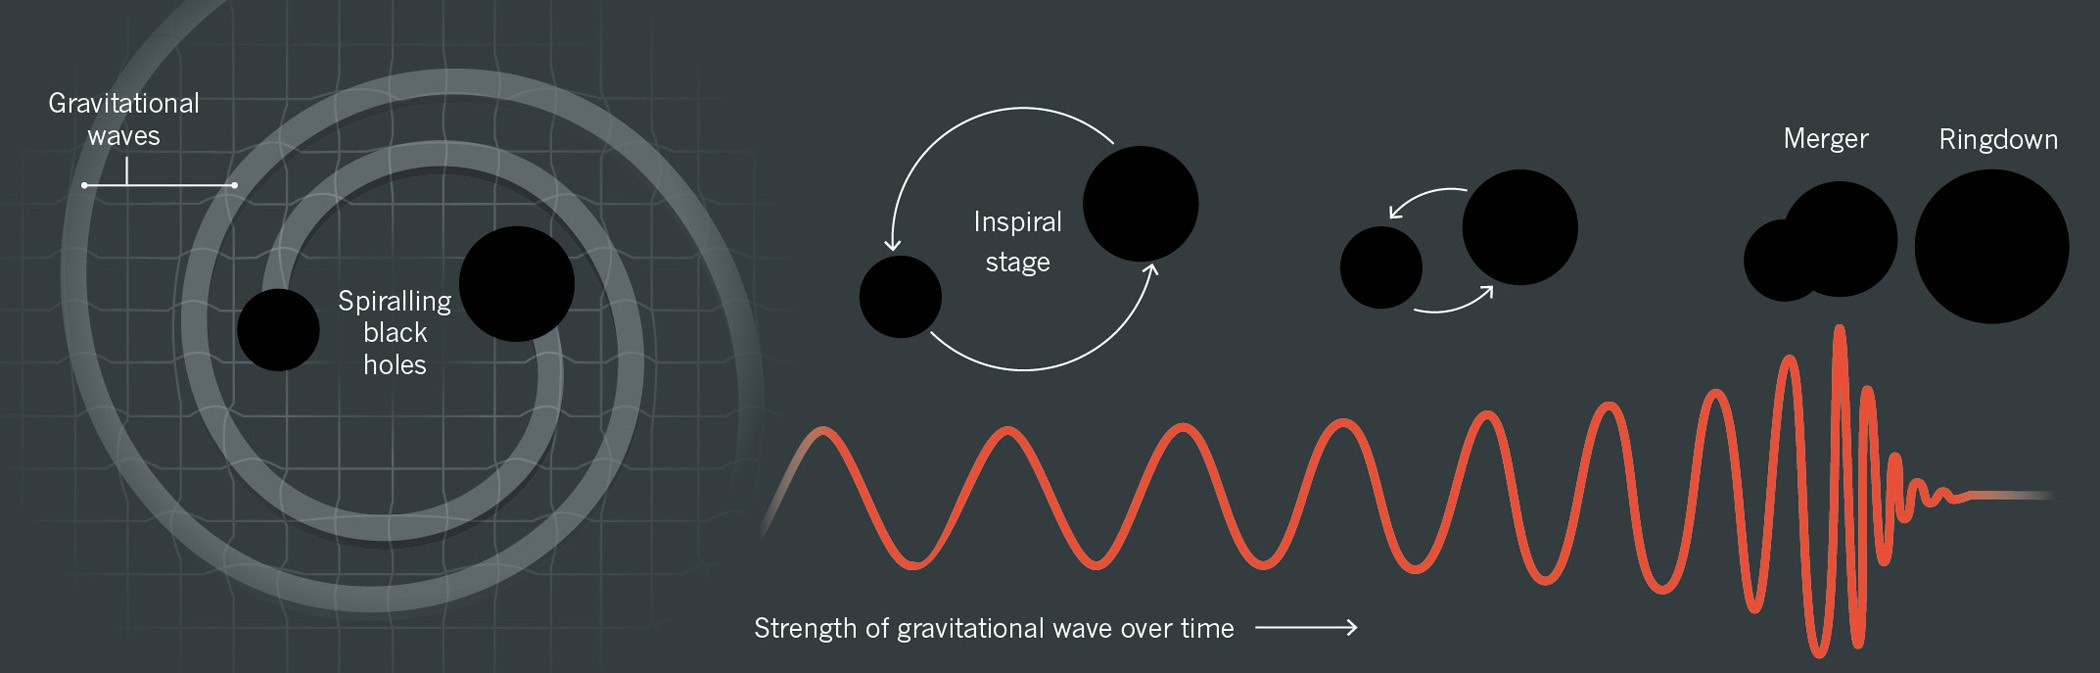
\includegraphics[width=0.73\linewidth]{Figures/inspiral_merger_ringdown.jpg}
    \caption{The three phases of a CBC: the inspiral, during which the two compact objects lose energy through GW emission and progressively approach each other; the merger, when the objects collide and coalesce; and the ringdown, in which the remnant settles into a stationary configuration by radiating the remaining perturbations. The corresponding gravitational waveform, showing the characteristic chirp of increasing frequency and amplitude, is displayed beneath each phase. Credit: Illustration by Lucy Reading-Ikkanda.}
    \label{fig:inspiral_merger_ringdown}
\end{figure}


These systems are classified as BBHs, binary neutron stars (BNS), or NS and BH binaries (NSBH). The emitted signal is driven by the time varying quadrupole moment and exhibits a characteristic chirp pattern, with increasing frequency and amplitude as the orbit shrinks. The duration of the detectable signal depends on the masses, ranging from fractions of a second for BBH mergers to much longer signals for BNS systems.

To date, nearly all GW detections made by ground based interferometers, including the LIGO Scientific Collaboration and the Virgo Collaboration, are consistent with CBC sources. During O1 and O2 \cite{O1_O2_catalog}, 11 events were identified, including the first BNS detection, GW170817 \cite{GW170817}. The number of detections increased significantly during O3 \cite{O3_catalog, O3_catalogue_part2} to around 90 events. During O4a \cite{O4a_catalog}, 128 new CBC candidates were identified, bringing the total to 218 when combined with previous catalogs, with binary BH mergers dominating the observed population.

The success in detecting CBCs is largely due to accurate waveform modelling, which enables matched filtering techniques to identify signals in noisy data. Future space based detectors such as the Laser Interferometer Space Antenna (LISA) (see $\S$\ref{spacebased_detectors}) will extend observations to other sources, including white dwarf binaries and extreme mass ratio inspirals (EMRIs), providing further insight into compact object populations and their formation \cite{EMRIs-WD}.


\subsection{Burst events}  
GW bursts are short duration signals produced by highly energetic and often poorly modelled astrophysical events. Typical sources include core collapse supernovae, gravitational collapses, highly eccentric compact binary mergers, and more speculative scenarios such as cosmic strings \cite{burst_events}. In addition, burst like emission can be associated with transient phenomena such as gamma ray bursts linked to NS or NS-BH mergers.

These signals typically last from a fraction of a second to a few tens of seconds and are characterized by their unpredictable morphology. Unlike CBCs or CWs, burst signals do not have accurate waveform models, which makes their detection more challenging. Instead of matched filtering techniques, searches rely on identifying excess power or coherent transients across multiple detectors \cite{monochromatic_CWs}.

\subsection{Continuous waves}

CWs are expected to be emitted by rapidly rotating compact objects, particularly NSs with small deviations from perfect axial symmetry. These asymmetries produce a time varying quadrupole moment, enabling the continuous emission of gravitational radiation. The resulting signal is nearly monochromatic, typically at a frequency related to the star’s rotation, and evolves very slowly due to spindown effects \cite{monochromatic_CWs}.

In contrast to CBCs, CW signals are extremely long lived but much weaker in amplitude, as they originate from small deformations in the source. As a result, their detection requires long observation times, often spanning months or years, in order to accumulate sufficient signal to noise ratio (SNR). Despite their low amplitude, once detected, these signals can be tracked over extended periods, allowing for precise studies of the source properties.

The strength of the emission depends on factors such as the rotation rate and internal structure of the NS, including its equation of state and crust properties \cite{CWs_source}. In addition to isolated NSs, other potential sources of CWs have been proposed, such as boson clouds \cite{Boson_clouds_CWs} around rapidly spinning BHs or compact binaries in very early inspiral stages. Although no CW signal has been confirmed so far, current searches have placed increasingly stringent upper limits, improving the prospects for future detections.


\subsection{Stochastic backgrounds}

SGWB is a diffuse signal produced by the superposition of many unresolved sources, which are either too weak or too numerous to be individually detected. This background can have both astrophysical and cosmological origins \cite{stochastic_backgrounds}. Astrophysical contributions arise from the cumulative effect of distant CBCs or populations of compact binaries such as WD systems, while cosmological contributions may be generated in the early Universe through processes such as inflation or phase transitions.


Although no definitive detection has yet been achieved by ground based detectors, current analyses have placed increasingly stringent upper limits on the energy density of the background \cite{detection_SGWB}. Detecting the SGWB would provide unique information about the population of unresolved sources and could offer a direct probe of physical processes in the early Universe, complementing observations of the cosmic microwave background.



\section{Detectors}


The first experimental attempts to detect GWs began in the 1960s with resonant-mass detectors, which aimed to measure the mechanical response of massive bars to passing waves \cite{ressonant_mass_detectors}. However, their limited sensitivity and narrow frequency range prevented successful detections. This motivated the development of interferometric detectors, capable of measuring extremely small changes in distance between test masses. After decades of technological progress, this approach led to the first direct detection of GWs in 2015 \cite{GW150914}.

Today, GW observations are routinely performed by a global network of ground-based interferometers, marking the beginning of GW astronomy.

\subsection{Interferometric detection principle}

Current GW detectors are based on laser interferometry, using a modified Michelson configuration, as illustrated in Fig.~\ref{fig:layout_LIGO}. A coherent laser beam is split into two perpendicular arms by a beam splitter. The light travels along each arm, is reflected by mirrors, and recombines at the beam splitter, producing an interference pattern that is measured by a photodetector \cite{Layout_LIGO}.

\begin{figure}[h!]
    \centering
    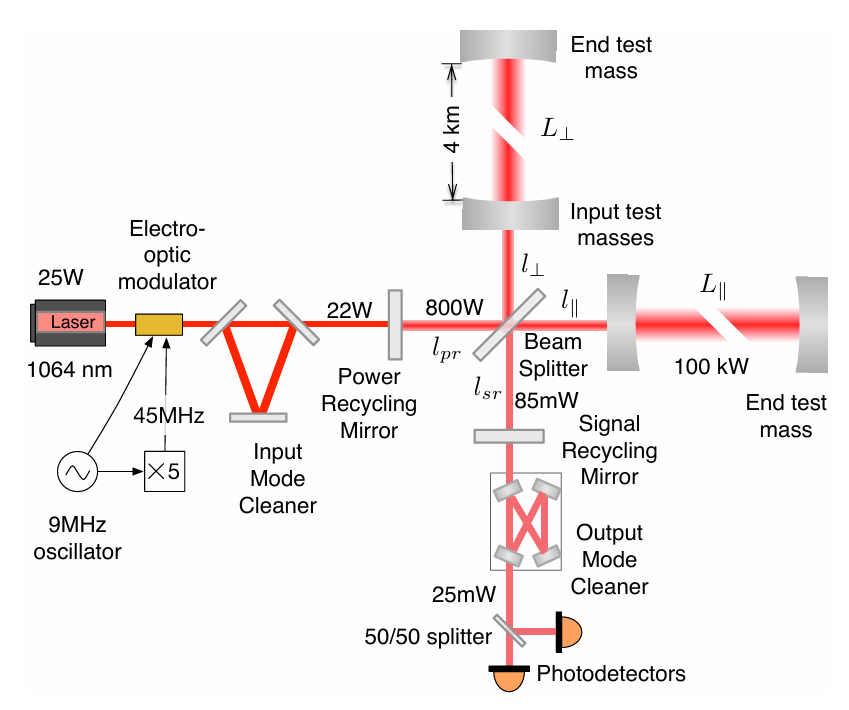
\includegraphics[width=0.73\linewidth]{Figures/Layout_LIGO.png}
    \caption{Optical layout of the advanced LIGO interferometer, illustrating the Fabry-Pérot arm cavities, the power recycling mirror (PRM) at the input port, and the signal recycling mirror (SRM) at the output port. Source: \cite{Layout_LIGO}.}
    \label{fig:layout_LIGO}
\end{figure}

In the absence of a GW, the lengths of the two arms are adjusted so that the interference at the output is destructive, resulting in minimal detected light. When a GW passes through the detector, it induces a differential stretching and compression of the arms, analogous to the tidal deformation described in \S\ref{geodesic_eq_sec} by the geodesic deviation equation \eqref{geodesicdeviation}. This changes the optical path lengths and produces a phase difference between the two beams, leading to a measurable signal at the photodetector.

The quantity measured is the strain $h(t)$, defined as the relative change in the arm lengths, $h \sim \Delta L / L$ (see \S\ref{antenna_patterns_sec}). This is precisely the quantity appearing in the TT metric perturbation \eqref{polarizationmodes}: the two polarization amplitudes $A_+$ and $A_\times$ directly set the scale of the fractional length change experienced by the detector arms. For typical detectors with arm lengths of a few kilometers, the expected variations are extremely small, of order $10^{-21}$, requiring highly sensitive instrumentation.

Modern interferometers incorporate several enhancements to increase their sensitivity. These include Fabry-Pérot cavities in the arms, which effectively increase the optical path length, and power and signal recycling mirrors, which enhance the circulating power and the detector response. Despite these improvements, the measurement remains extremely challenging due to the tiny magnitude of the effect, set ultimately by the quadrupole formula discussed in \S\ref{quadrupole_sec} and the astrophysical distances involved.


\subsection{Detector response}

The response of an interferometric detector depends on the relative orientation between the incoming GW and the detector arms. This is described by antenna pattern functions, which determine the sensitivity to different sky locations and polarization states. As a result, a single detector has limited directional sensitivity, making a network of detectors essential for accurate sky localization and PE.


\subsubsection{Antenna pattern of a ground-based interferometric detector}
\label{antenna_patterns_sec}

Here we derive the response of a ground-based Michelson interferometer to a plane GW in the long-wavelength approximation, where the detector arm length is much smaller than the reduced wavelength of the wave. 


A complete description of the detection problem requires three distinct Cartesian frames \cite{TriasCornellana2011GW}. The wave frame $(x',y',z')$ has its $z'$-axis aligned with the propagation direction; in this frame the TT metric perturbation takes the standard form 
\begin{equation}
H =
\begin{pmatrix}
h_+ & h_\times & 0 \\
h_\times & -h_+ & 0 \\
0 & 0 & 0
\end{pmatrix},
\label{strain_tensor}
\end{equation}
where $h_+$ and $h_\times$ denote the plus and cross polarizations.
The detector frame $(\bar{x},\bar{y},\bar{z})$ has its $\bar{z}$-axis pointing toward the local zenith and the two arms lying in the $(\bar{x},\bar{y})$ plane along unit vectors $\hat{\mathbf{n}}_1$ and $\hat{\mathbf{n}}_2$, separated by an opening angle $\zeta$. Finally, an ecliptic frame $(x,y,z)$ centered at the Solar System Barycenter serves as a common inertial reference for source localization. The relative orientation of the wave and detector frames is parametrized by the polar angles $(\bar{\theta}_N, \bar{\phi}_N)$ specifying the source direction in the detector frame, and the polarization angle $\psi$ (see Fig.~\ref{fig:antennapatternscoord}).

\begin{figure}[h!]
    \centering
    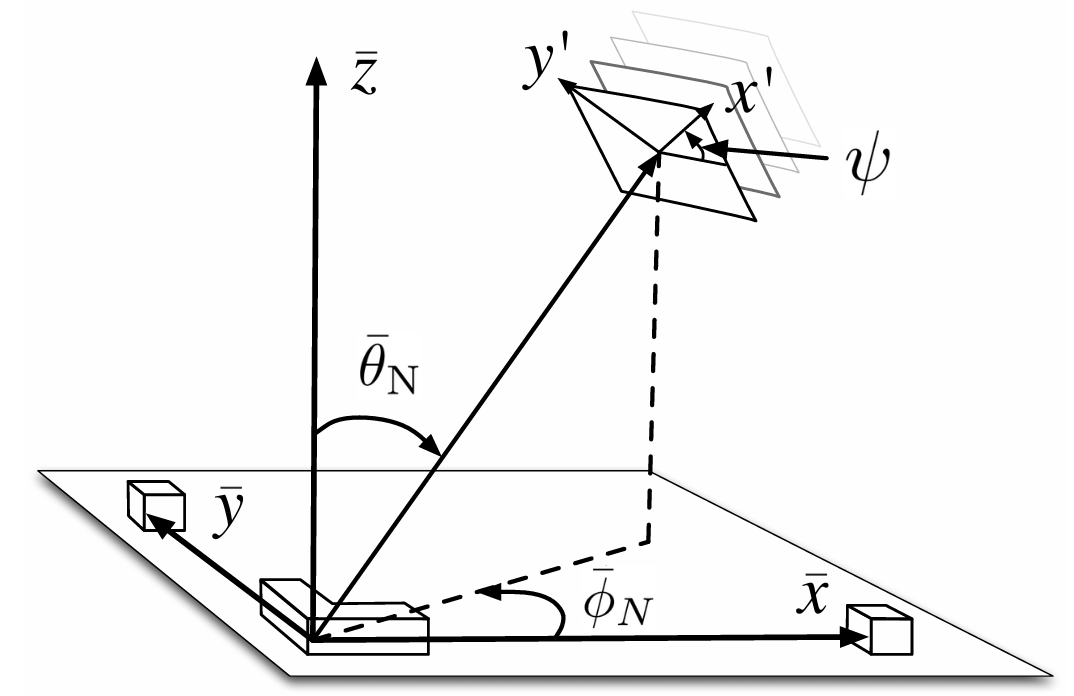
\includegraphics[width=0.57\linewidth]{Figures/antennapatterncoordinates.png}
    \caption{Geometric relationship between the detector frame $(\bar{x},\bar{y},\bar{z})$ and the wave frame $(x',y',z')$. The interferometer arms lie in the $(\bar{x},\bar{y})$ plane, with $\bar{z}$ pointing toward the local zenith. The angles $\bar{\theta}_N$ and $\bar{\phi}_N$ give the polar and azimuthal coordinates of the incoming wave direction in the detector frame, and $\psi$ denotes the rotation of the polarization axes about the propagation direction. Own production based on the source: \cite{ABADIE2010223}.}
    \label{fig:antennapatternscoord}
\end{figure}


The observable quantity is the differential arm-length variation induced by the passing wave. Working to first order in $h$ and applying the geodesic deviation equation \eqref{eq:geodesiceq} in the detector frame, the fractional length change of a single arm oriented along 
$\hat{\mathbf{n}}$ is
\begin{equation}
    \frac{\delta L(t)}{L} = \frac{1}{2}\,\hat{\mathbf{n}}^{T}
    \tilde{H}(t)\,\hat{\mathbf{n}},
\end{equation}
where $\tilde{H}(t) = M H(t) M^T$ is the wave-frame strain tensor \eqref{strain_tensor} rotated into the detector frame by the orthogonal matrix $M$. The scalar strain measured by the interferometer is then
\begin{equation}
    h(t)= \frac{\Delta L_{\text{arms}}(t)}{L}=\frac{L_1(t)-L_2(t)}{L}=\frac{\delta L_1(t)}{L}-\frac{\delta L_2(t)}{L}=\frac{1}{2}\,\hat{\mathbf{n}}_1^T \cdot \tilde{H}(t)\,\hat{\mathbf{n}}_1 - \frac{1}{2}\,\hat{\mathbf{n}}_2^T \cdot \tilde{H}(t)\,\hat{\mathbf{n}}_2 ,
    \label{eq:strain_detector}
\end{equation}
where the sign convention follows from choosing 
$\hat{\mathbf{n}}_1 \times \hat{\mathbf{n}}_2$ to point outward from the Earth's surface \cite{PhysRevD.58.063001}.

The frame transformation is given by the sequence of Euler rotations
\begin{equation}
    M = R_z(-\bar{\phi}_N)\,R_y(-\bar{\theta}_N+\pi)\,R_z(\psi),
\end{equation}
which encodes both the sky location of the source and the orientation of the polarization axes relative to the detector.


Substituting the explicit form of $M$ and the arm vectors into \eqref{eq:strain_detector}, and simplifying with standard trigonometric identities, the detector response takes the form
\begin{equation}
    h(t) = F_{+}(\psi,\zeta,\bar{\theta}_N,\bar{\phi}_N)\,h_+(t)
          + F_{\times}(\psi,\zeta,\bar{\theta}_N,\bar{\phi}_N)\,h_\times(t),
    \label{eq:hoft}
\end{equation}
where the antenna pattern functions are \cite{TriasCornellana2011GW, 
PhysRevD.58.063001}
\begin{align}
F_{+} &= \sin\zeta\left[
    \frac{1}{2}(1+\cos^2\bar{\theta}_N)\cos 2\bar{\phi}_N\cos 2\psi
    - \cos\bar{\theta}_N\sin 2\bar{\phi}_N\sin 2\psi
    \right], \label{eq:Fplus} \\[4pt]
F_{\times} &= -\sin\zeta\left[
    \frac{1}{2}(1+\cos^2\bar{\theta}_N)\cos 2\bar{\phi}_N\sin 2\psi
    + \cos\bar{\theta}_N\sin 2\bar{\phi}_N\cos 2\psi
    \right]. \label{eq:Fcross}
\end{align}
These expressions satisfy the symmetry relations
\begin{equation}
    F_{+}\!\left(\psi+\tfrac{\pi}{4}\right) = F_{\times}(\psi),
    \qquad
    F_{+,\times}\!\left(\psi+\tfrac{\pi}{2}\right) = -F_{+,\times}(\psi),
\end{equation}
reflecting the spin-2 character of GWs: a $\pi/4$ rotation of the polarization angle exchanges the two modes, while a $\pi/2$ rotation reverses their sign.

A polarization-independent measure of the directional sensitivity is provided by the quadrature sum
\begin{equation}
    |F| = \sqrt{F_+^2 + F_\times^2},
\end{equation}
shown in Fig.~\ref{fig:antennapatternsavg} for $\zeta=\pi/2$. The characteristic quadrupolar structure reflects the tensorial nature of the GW strain and the geometric projection onto the detector arms. The individual patterns $F_+$ and $F_\times$ are displayed in 
Fig.~\ref{fig:antennapatternsFxFplus} for several values of $\psi$; each successive column corresponds to a $\pi/8$ increment in polarization angle, illustrating the interchange symmetry above.

\begin{figure}[h!]
    \centering
    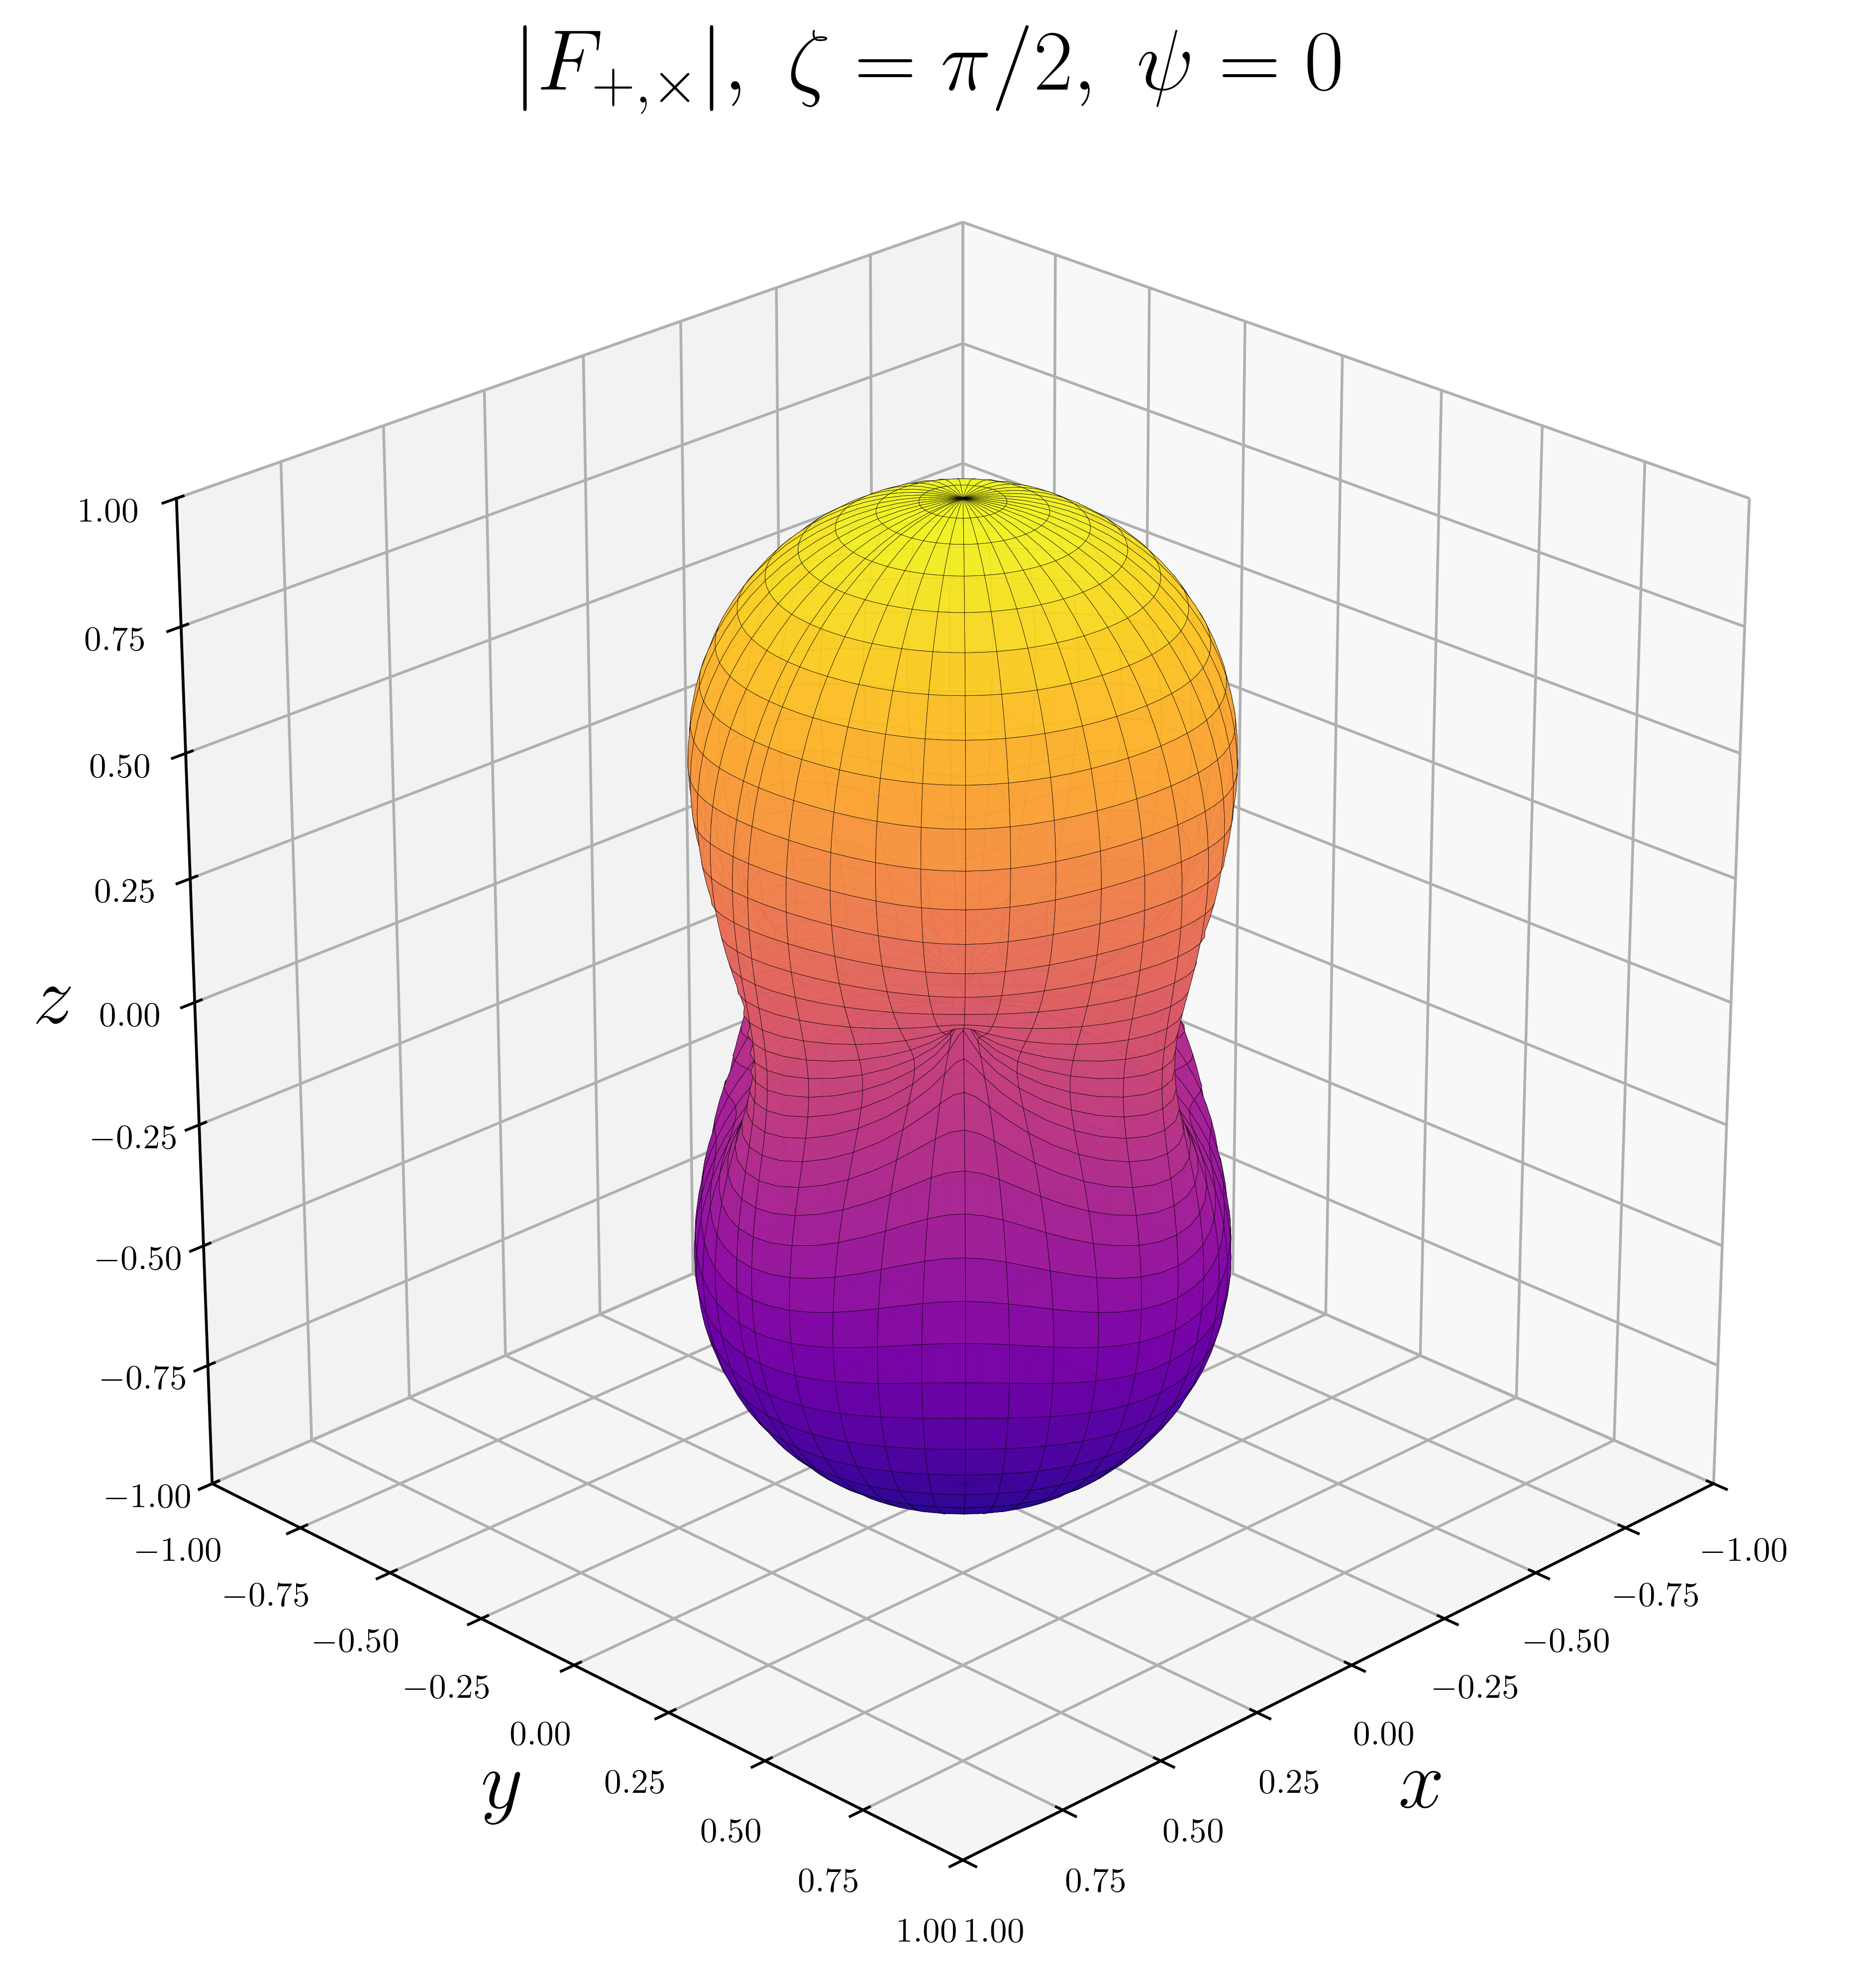
\includegraphics[width=0.47\linewidth]{Figures/antenna_patterns_averaged.png}
    \caption{Polarization-averaged antenna pattern $|F|$ of a ground-based interferometer with orthogonal arms ($\zeta=\pi/2$), as a function of sky angles $(\bar{\theta}_N,\bar{\phi}_N)$. Original result.}
    \label{fig:antennapatternsavg}
\end{figure}

\begin{figure}[h!]
    \centering
    \includegraphics[width=0.96\linewidth]{Figures/antenna_patterns_Fx_F+.png}
    \caption{Antenna patterns for the plus ($F_+$, top) and cross ($F_\times$, bottom) polarizations for $\zeta=\pi/2$ and representative values of $\psi$. Original result.}
    \label{fig:antennapatternsFxFplus}
\end{figure}


\subsection{Noise and sensitivity}
\label{sec:noise}

A GW with strain $h \sim 10^{-21}$ produces a differential arm-length change $\delta L = hL/2 \sim 10^{-18}$\,m for $L = 4$\,km, three orders of magnitude smaller than the diameter of a proton. Achieving sensitivity at this level requires identifying and suppressing a broad set of noise sources that would otherwise overwhelm the signal. These are conveniently characterised by the one-sided power spectral density (PSD) $S_n(f)$ \cite{PSD_book}, defined as the Fourier transform of the autocorrelation function\footnote{
The autocorrelation function measures how strongly a signal is correlated with a delayed version of itself as a function of the time lag $\tau$. In the context of detector noise, it quantifies the degree to which noise fluctuations at different times remain statistically related \cite{autocorrelation_function}.
} of the detector output: 
\begin{equation}
    S_n(f) = \int C(\tau)\, e^{-i 2\pi f \tau} \, d\tau ,
\label{PSD_eq}
\end{equation}
where $C(\tau) = \langle n(t) n(t+\tau) \rangle$ is the autocorrelation function of the noise process $n(t)$, and $\langle \cdot \rangle$ denotes an ensemble average.
Its square root $\sqrt{S_n(f)}$, expressed in units of Hz$^{-1/2}$, defines the sensitivity curve of the instrument and sets the threshold below which signals are inaccessible.



Noise sources are broadly divided into two categories. 
Fundamental noise arises directly from the measurement principle and cannot be removed without redesigning the detector. Technical noise is not intrinsic to the design but still limits performance. The main contributions are the following \cite{noise_aLIGO,noise_budget_O4}:

\begin{itemize}

    \item \textbf{Shot noise.} The Poissonian arrival statistics of photons at the output photodetector produce a phase uncertainty scaling as $1/\sqrt{N_\gamma}$, where $N_\gamma$ is the number of detected photons per unit time. This contribution decreases with increasing circulating power and dominates the sensitivity above $\sim\!200$\,Hz. It can be partially mitigated by injecting squeezed vacuum at the output port, a technique already incorporated 
    in the Advanced LIGO and Advanced Virgo detectors.

    \item \textbf{Radiation-pressure noise.} Amplitude fluctuations of the intracavity field exert a stochastic force on the mirror surfaces, inducing position noise that grows with laser power and becomes significant at low frequencies. Shot noise and radiation-pressure noise are related by the Heisenberg uncertainty principle and together define the standard quantum limit for a free test mass. Squeezed-light injection redistributes the quantum uncertainty between the two quadratures, allowing simultaneous reduction of both contributions below the standard quantum limit.

    \item \textbf{Thermal noise.} Any component at finite temperature undergoes stochastic mechanical motion. Via the fluctuation-dissipation theorem\footnote{The fluctuation-dissipation theorem states that any dissipative mechanism in a system in thermal equilibrium is necessarily accompanied by a fluctuating force of the same origin. In interferometric detectors, mechanical losses in the test masses, coatings, and suspension fibers therefore set a fundamental limit on their positional stability \cite{Kubo1966}.}, the amplitude of these fluctuations is proportional to the mechanical loss angle of the material. It affects the test masses, their dielectric mirror coatings, and the suspension fibers, and dominates the sensitivity in the intermediate band of roughly $40$-$200$\,Hz. Low-loss fused-silica substrates and fibers are employed to minimize this contribution; cryogenic operation, as adopted by KAGRA, provides an alternative route to its suppression.

    \item \textbf{Seismic noise.} Ground motion couples mechanically to the test masses through the suspension chain. The quadruple-pendulum isolation system attenuates seismic vibrations by more than ten orders of magnitude above $\sim\!10$\,Hz, but residual motion from microseisms, wind, and anthropogenic activity still limits the sensitivity below $\sim\!40$\,Hz.

    \item \textbf{Newtonian noise.} Density fluctuations in the surrounding ground and atmosphere produce direct gravitational forces on the test masses that cannot be shielded mechanically. This contribution, also known as gravity-gradient noise, sets a fundamental floor at low frequencies for surface-based detectors. 


    \item \textbf{Control noise.} Servo loops are required to maintain the arm cavities on resonance and keep the optical components aligned. The sensors and actuators in these feedback systems introduce noise that couples into the GW channel, representing the dominant technical limitation at low frequencies.

    \item \textbf{Residual gas noise.} Despite the ultra-high vacuum environment ($<1\,\mu$Pa in the beam tubes), residual molecules scatter laser photons and cause fluctuations in the optical path length. This contribution is generally subdominant but must be controlled to avoid limiting the sensitivity in specific frequency bands.

    \item \textbf{Other technical noise sources.} Laser frequency and intensity fluctuations, electromagnetic coupling, scattered light, and photodetector dark noise contribute across various frequency ranges. These are monitored and subtracted using a network of 
    $\gtrsim\!2\times10^5$ auxiliary channels (including magnetometers, accelerometers, microphones and photodetectors) that record the state of the instrument and its environment continuously.

\end{itemize}

The noise process is approximately Gaussian but not stationary. Two classes of artefact further degrade the data quality. Lines are persistent narrow-band features visible as peaks above the noise floor in the PSD, arising from power-line harmonics (50 or 60\,Hz and their multiples), mirror suspension violin modes, calibration injections, and environmental electromagnetic coupling (see Fig.~\ref{fig:lines_noise}) \cite{lines_noise}. 

\begin{figure}[h!]
    \centering
    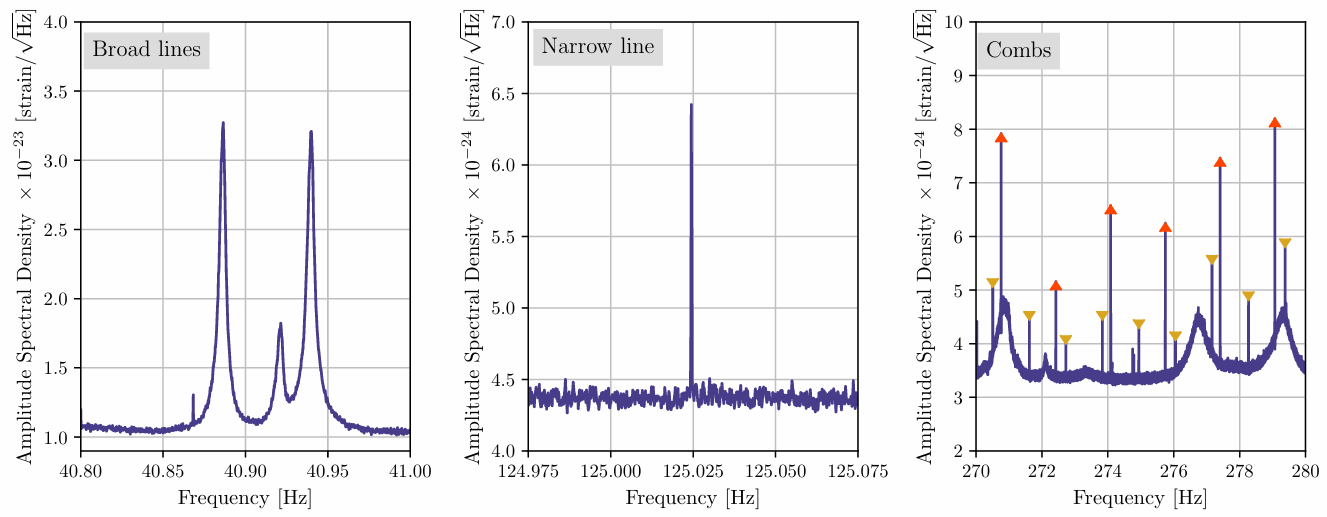
\includegraphics[width=0.84\linewidth]{Figures/narrow_lines.png}
    \caption{High-resolution amplitude spectral density ($\Delta f = 1/1800$\,Hz) of LIGO Hanford strain data illustrating three representative line artefacts. Left: a broad spectral feature associated with mirror suspension roll-mode resonances. Centre: an isolated narrow line of unknown origin. Right: two frequency combs with distinct spacings, marked by upright and inverted triangles, alongside broader noise structures. Source: \cite{glitches_lines_noises}.}
    \label{fig:lines_noise}
\end{figure}


Glitches are short-duration transient bursts of excess power whose morphology can mimic astrophysical signals, reducing the efficiency of detection pipelines (see Fig.~\ref{fig:glitches_noise}) \cite{Glitches}.

\begin{figure}[h!]
    \centering
    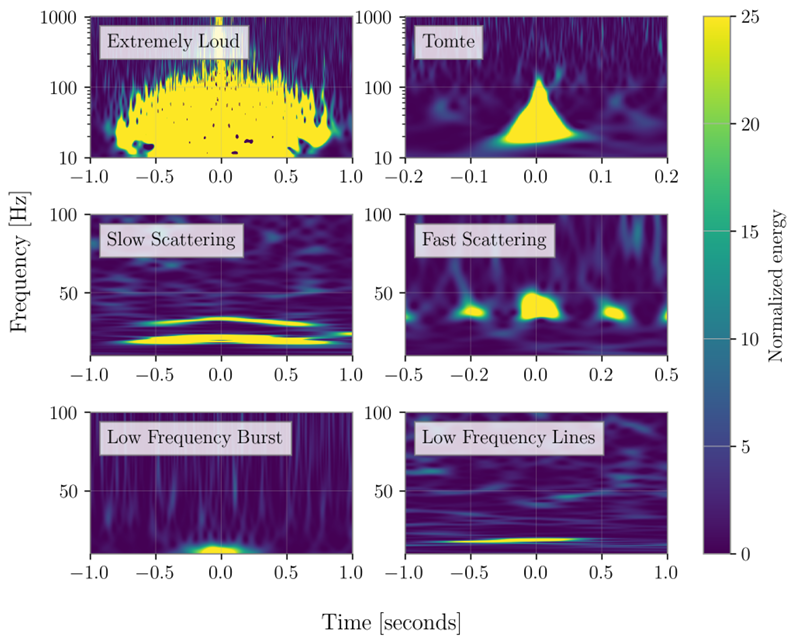
\includegraphics[width=0.75\linewidth]{Figures/glitches.png}
    \caption{Time-frequency spectrograms of representative glitch classes recorded at LHO and LLO. Slow and Fast Scattering artefacts are attributed to light scattered by optics under increased ground motion, while the origin of Extremely Loud, Tomte, Low Frequency Burst, and Low Frequency Lines glitches remains unidentified. Source: \cite{glitches_lines_noises}.}
    \label{fig:glitches_noise}
\end{figure}


The interplay of all these contributions shapes the detector sensitivity curve shown in Fig.~\ref{fig:noise_budget}, where three distinct regimes are clearly visible: control and seismic noise below $\sim\!50$\,Hz, a combination of thermal and quantum noise in the intermediate band ($50$-$500$\,Hz), and shot noise above $\sim\!500$\,Hz. Together they define the accessible frequency range of $\sim\!10$-$5000$\,Hz for current ground-based detectors. The sharp spectral peaks superimposed on the broadband noise floor correspond to the lines discussed above, most prominently the 60\,Hz power-line harmonic and the mirror suspension violin modes.

\begin{figure}[h!]
    \centering
    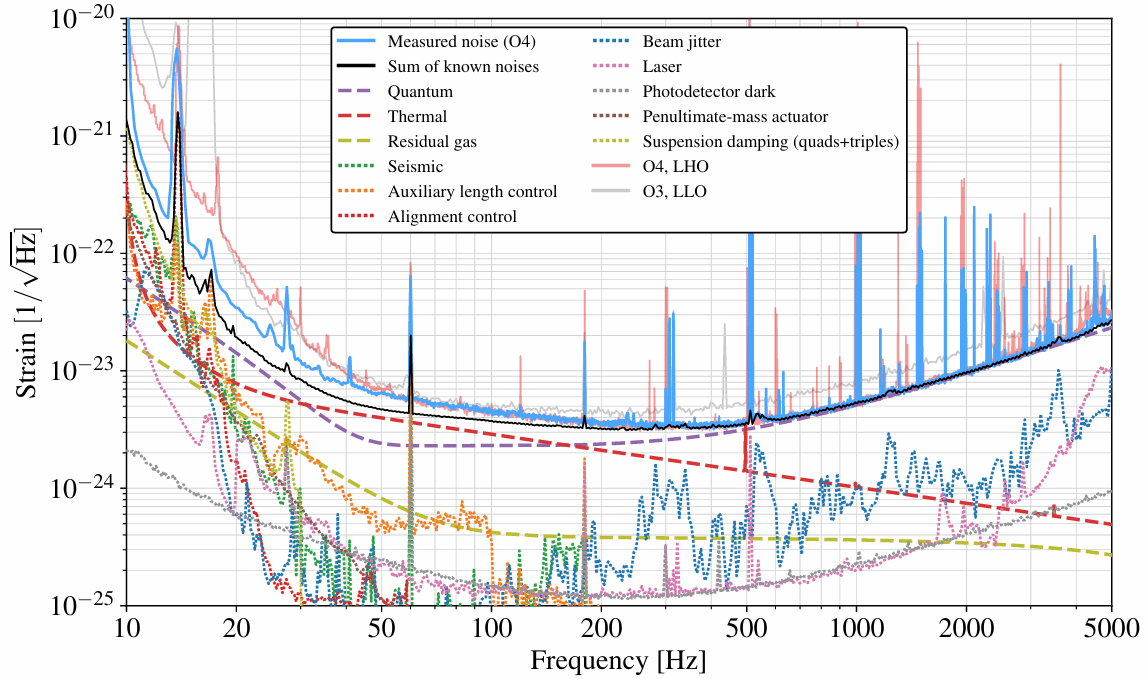
\includegraphics[width=0.79\linewidth]{Figures/noise_budget_O4_LLO.png}
    \caption{Strain noise amplitude spectral density of the LLO detector during O4, together with the O3 LLO and O4 LHO curves for comparison. Dashed lines indicate noise contributions estimated from analytical models or independent component measurements; dotted lines correspond to noise projected from auxiliary witness channels. The black curve gives the quadrature sum of all known noise sources. Three regimes are apparent: control noise dominates below $\sim\!50$\,Hz, a combination of quantum and thermal noise governs the intermediate band, and shot noise sets the high-frequency floor above $\sim\!500$\,Hz. Narrow spectral lines from power-line harmonics, violin modes, and calibration injections are visible throughout the spectrum. Source: \cite{noise_budget_O4}.}
    \label{fig:noise_budget}
\end{figure}



\subsection{Current detector network}


A single interferometer provides limited directional information: the antenna pattern functions derived in \S\ref{antenna_patterns_sec} show that a ground-based detector is nearly blind along certain sky directions. A global network of detectors is therefore essential, both to confirm detections through coincident observations and to localise 
sources on the sky via time delay triangulation. Sky localisation precision improves with the number of detectors, their mutual separation, and their individual sensitivities. The current network consists of four facilities operating in the frequency band $\sim\!10$-$5000$\,Hz (see Fig.~\ref{fig:current_network}):

\begin{itemize}

    \item \textbf{Advanced LIGO} \cite{Advanced_ligo} 
    comprises two 4-km detectors: LIGO Hanford (H1) in Washington State and LIGO Livingston (L1) in Louisiana, separated by $\sim\!3000$\,km. Operated by the LIGO Scientific Collaboration (LSC), they have been the primary instruments for GW detections 
    since the first observation of a BBH merger in September 2015 \cite{GW150914}. A third Advanced LIGO detector, LIGO-India, is currently under construction and expected to join the network in 2030.

    \item \textbf{Advanced Virgo (V1)} \cite{Advanced_VIRGO} is a 3-km interferometer located in Cascina, Italy, operated by the Virgo Collaboration. It joined the network in the final month of O2, contributing to the first three-detector observation of a BBH merger (GW170814 \cite{GW170814}) and to the precise sky localisation of the BNS merger GW170817 \cite{GW170817}. Although its sensitivity is somewhat below that of the LIGO instruments, its geographic separation from the US sites significantly improves source localisation.

    \item \textbf{KAGRA (K1)} \cite{KAGRA} is a 3-km cryogenic underground detector situated 200\,m beneath the Kamioka mountain in Gifu Prefecture, Japan. Its subterranean location provides natural seismic and atmospheric shielding, and its test masses are cooled to cryogenic temperatures ($\sim\!20$\,K) to suppress thermal noise, making it the first second-generation detector to adopt this approach. KAGRA participated in a short joint observing run with GEO600 at the end of O3, and has been part of the network since O4.

    \item \textbf{GEO600} \cite{GEO600} is a 600-m detector near Hannover, Germany, operated jointly by British and German institutions. Its shorter arms make it significantly less sensitive than the kilometre-scale instruments, so it does not contribute to standard astrophysical searches. Instead, it operates in astrowatch mode during maintenance periods of the other detectors and serves as a testbed for advanced instrumentation techniques (including squeezed-light injection) before their deployment in larger facilities. GEO600 is scheduled to conclude operations in 2026, marking the end of its role as the longest-running interferometric GW detector in Europe.

\end{itemize}


\begin{figure}[h!]
    \centering
    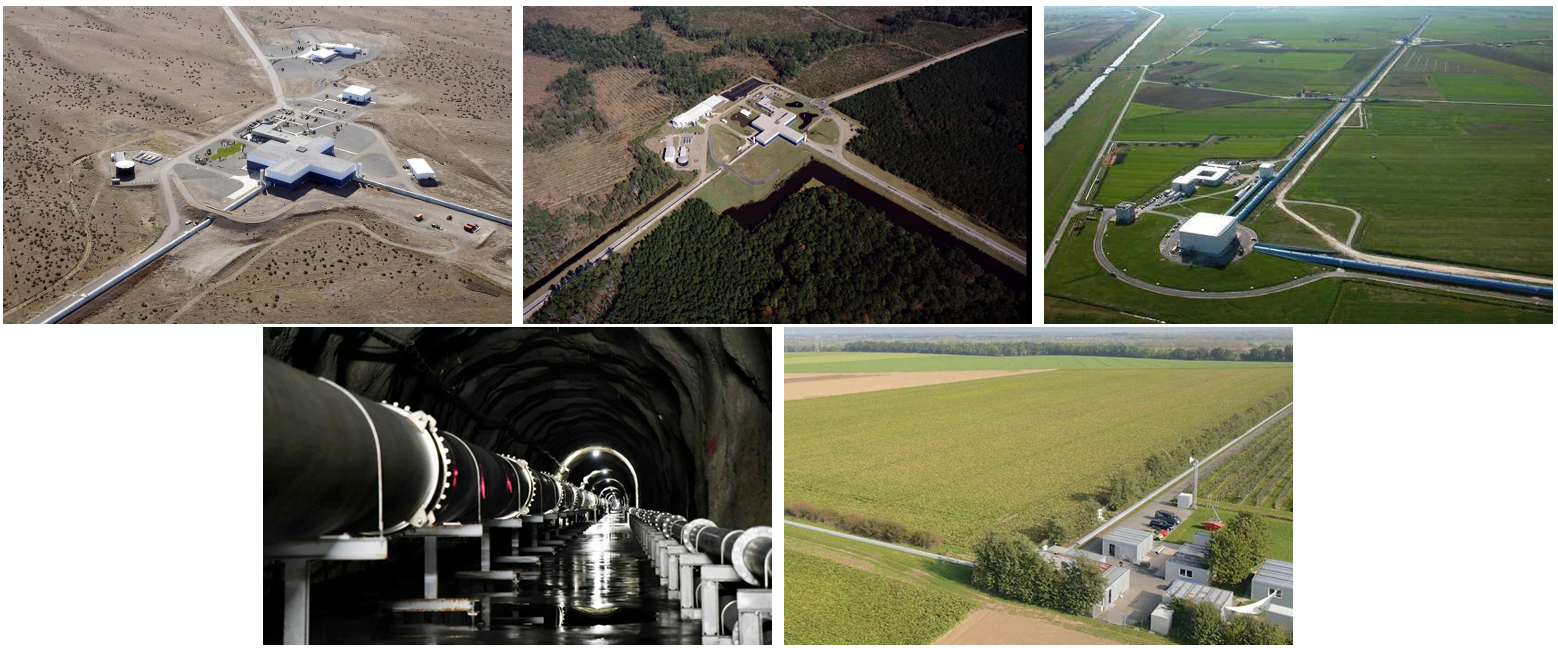
\includegraphics[width=0.85\linewidth]{Figures/current_network_interferometers.png}
    \caption{Aerial and underground views of the current LVK detector network. Top row, left to right: LIGO Hanford (Washington, USA), LIGO Livingston (Louisiana, USA), and Advanced Virgo (Cascina, Italy). Bottom row, left to right: KAGRA underground tunnel (Kamioka, Japan) and GEO600 (Hannover, Germany). Sources: \cite{HANFORD, LIGO_Livingston_image, eoportal_virgo,asiop_kagra,geo600_website}.}
    \label{fig:current_network}
\end{figure}


The evolution of the network across observing runs is illustrated in Fig.~\ref{fig:runs_O1234}. During O1 and the majority of O2, only H1 and L1 were operational; Virgo joined for the final weeks of O2 and participated throughout O3. A brief joint run (O3GK) at the close of O3 included GEO600 and KAGRA. Since O4, the network comprises all four facilities, with the BNS inspiral range (the standard figure 
of merit for detector sensitivity) improving progressively across runs as a result of the upgrades discussed in 
\S\ref{sec:noise}.

\begin{figure}[h!]
    \centering
    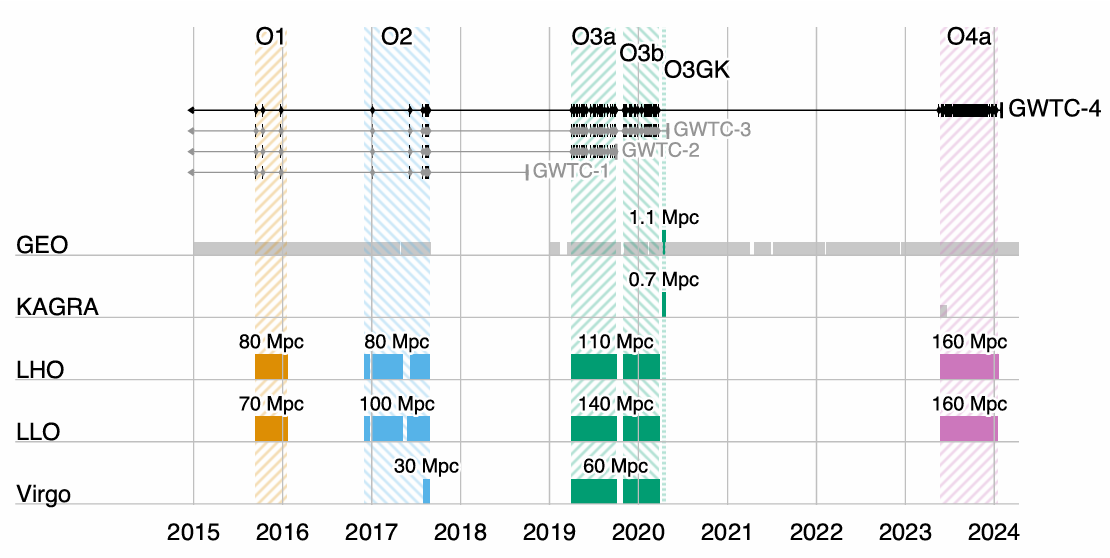
\includegraphics[width=0.785\linewidth]{Figures/Runs_timeline.png}
    \caption{Timeline of LVK observing runs from the first detection in 2015 through O4a. Colored bars indicate the periods during which each detector was operating, together with the typical BNS inspiral range achieved in each run. GEO astrowatch and KAGRA O4a periods (light gray) were not included in the main GW analyses. Virgo joined the network in the final month of O2 and operated throughout O3; a short joint O3GK run also included GEO600 and KAGRA. Tick marks along the top indicate GW candidates from GWTC-1 through GWTC-4 with astrophysical probability $\geq 50\%$. Source: \cite{runs_timeline_O1234}.}
    \label{fig:runs_O1234}
\end{figure}



\subsection{Future detectors}
\label{sec:future_detectors}

The current LVK network has demonstrated the transformative potential of GW astronomy, but its sensitivity and frequency coverage remain limited by fundamental and technical noise sources discussed in \S\ref{sec:noise}. The next generation of detectors, both ground-based and space-based, aims to extend the accessible parameter space by one to two orders of magnitude in strain sensitivity and to cover a much broader frequency band.

\subsubsection{Ground-based third-generation detectors.}

\begin{itemize}
    \item   \textbf{Einstein Telescope} (ET) \cite{Einsteintelescope} is the European third-generation concept, designed as an equilateral triangle with 10-km arms hosted underground to suppress seismic and Newtonian noise. Each side hosts a xylophone configuration: two nested interferometers, one optimised for high frequencies at room temperature and one for low frequencies operating cryogenically, jointly covering the band $\sim\!2$-$10^4$\,Hz. The triangular geometry provides full sky coverage and allows simultaneous measurement of both GW polarizations with a single facility.
    \item \textbf{Cosmic Explorer} (CE) \cite{evans2021horizonstudycosmicexplorer} is the US counterpart, conceived as an L-shaped interferometer with 40-km arms (roughly ten times the length of Advanced LIGO) retaining the proven Michelson topology while achieving a strain sensitivity improvement of approximately one order of magnitude. Together, ET and CE would form a third-generation network capable of detecting CBC mergers throughout the majority of the observable Universe.
    \item \textbf{LIGO India} \cite{LIGO_INDIA} is a planned Advanced LIGO-class detector to be built in Maharashtra, India. Although it will not exceed the sensitivity of the current LIGO instruments, its geographic location will substantially improve sky localisation and detection confidence for the global network.
\end{itemize}


\subsubsection{Space-based detectors.}
\label{spacebased_detectors}
Ground-based detectors are fundamentally limited below $\sim\!10$\,Hz by seismic and Newtonian noise. Space-based missions overcome this barrier by operating in a quiet gravitational environment, opening the mHz frequency window inaccessible from the ground.

\begin{itemize}
    \item \textbf{LISA} \cite{LISA_detector} is the flagship ESA mission, scheduled for launch in the mid-2030s. It consists of three spacecraft in heliocentric orbit forming a near-equilateral triangle with $2.5\times10^6$\,km arms. Because the arm lengths are unequal and variable, standard Michelson cancellation of laser frequency noise is not possible; instead, Time Delay Interferometry (TDI) is employed to suppress this noise in post-processing. LISA will cover the band $\sim\!10^{-4}$--$10^{-1}$\,Hz, giving access to sources including massive BH mergers, EMRIs, and the early inspiral of compact binaries centuries before they enter the ground-based band. The feasibility of the key technologies was demonstrated by the LISA Pathfinder mission in 2015-2017.
\end{itemize}

Further space-based concepts under study include the Japanese 
DECIGO \cite{DECIGO_detector}, targeting the decihertz band ($\sim\!0.1$-$10$\,Hz) that bridges LISA and ground-based detectors, and the Chinese missions TianQin and Taiji \cite{TianQin_detector}, which share a similar frequency range to LISA with different orbital configurations.

The combination of third-generation ground-based detectors and space-based observatories is expected to provide continuous frequency coverage from $\sim\!10^{-4}$\,Hz to several kHz by the late 2030s, enabling a new era of multi-band GW astronomy.


\section{Gravitational wave data analysis}
\label{sec:data_analysis}

The preceding sections established the theoretical framework for GW generation and propagation, and the experimental techniques employed to detect them. The remaining challenge is to extract astrophysical information from the noisy output of the detectors. This requires combining signal processing, physical modelling, and statistical 
inference. The workflow proceeds in three stages: first, matched filtering is used to identify candidate events buried in the noise ($\S$\ref{sec:matched_filtering}); second, accurate waveform models are needed to compare against the data ($\S$\ref{sec:waveform_models}); and third, Bayesian PE is applied to the detected signal to infer the properties of the source ($\S$\ref{sec:PE}).

\subsection{Matched filtering and signal-to-noise ratio}
\label{sec:matched_filtering}

\subsubsection{Detector output and noise model}

The output of a GW detector can be written as the sum of a 
GW signal and instrumental noise,
\begin{equation}
    s(t) = h(t;\boldsymbol{\theta}) + n(t),
    \label{eq:detector_output}
\end{equation}
where $h(t;\boldsymbol{\theta})$ is the GW strain parametrized by the source parameters $\boldsymbol{\theta}$, and $n(t)$ is the noise contribution. With the sensitivity of current detectors, the noise amplitude is several orders of magnitude larger than the signal, $|h(t;\boldsymbol{\theta})| \ll |n(t)|$, so a detection cannot be claimed by direct inspection of $s(t)$ \cite{maggiore2007gravitational}. A systematic method is therefore required to extract the buried signal.

Although the true noise is non-stationary and non-Gaussian (exhibiting glitches and spectral lines as discussed in 
\S\ref{sec:noise}) a tractable analytic framework is obtained by modelling it as a zero-mean, stationary Gaussian random process fully characterized by its one-sided power spectral density (PSD) 
$S_n(f)$ \eqref{PSD_eq},
\begin{equation}
    \langle \tilde{n}^*(f)\,\tilde{n}(f') \rangle 
    = \frac{1}{2}\,S_n(f)\,\delta(f - f'),
    \label{eq:PSD}
\end{equation}
where tildes denote Fourier transforms, $\delta(f-f')$ is the Dirac delta encoding the statistical independence of different frequency components, and $\langle\cdot\rangle$ denotes an ensemble average, which for a single detector is identified with a time average via the ergodic theorem\footnote{The ergodic theorem states that, for a stationary random process, time averages computed from a single sufficiently long realization are equivalent to ensemble averages over all possible realizations. In practice, this means that the PSD $S_n(f)$ can be 
estimated directly from a single stretch of detector data, for example via the Welch method, without requiring multiple independent noise realizations.}. Under this Gaussian noise model, the probability density of a noise realization $n(t)$ is
\begin{equation}
    p(n) \propto \exp\!\left(-\frac{1}{2}(n|n)\right),
\end{equation}
where we have introduced the noise-weighted inner product (Wiener scalar product) between two real time series $a(t)$ and 
$b(t)$,
\begin{equation}
    (a|b) \equiv 4\,\mathrm{Re}\int_0^\infty 
    \frac{\tilde{a}^*(f)\,\tilde{b}(f)}{S_n(f)}\,df.
    \label{eq:inner_product}
\end{equation}
This inner product weights frequency bins inversely by the noise power, so that frequency bands where the detector is more sensitive contribute more to the overlap between two waveforms.

\subsubsection{The matched filter and optimal SNR}

Given a template waveform $h_m(t;\boldsymbol{\theta})$ representing our best theoretical model of the expected signal (see $\S$\ref{sec:waveform_models}), the matched filter is the linear filter $K(t)$ that maximizes the SNR. The SNR is defined as the ratio of the expected filtered output when a signal is present to the root-mean-square of the filtered output when only noise is present. Concretely, one filters the detector output by computing the scalar product
\begin{equation}
    \hat{s} = \int_{-\infty}^{\infty} s(t)\,K(t)\,dt,
\end{equation}
and seeks the $K(t)$ that maximizes the ratio of the expected value of $\hat{s}$ when a signal is present to the root-mean-square of $\hat{s}$ when only noise is present. Applying the Cauchy-Schwarz inequality to this optimization in the frequency domain, one finds that the optimal filter is proportional to the signal template weighted by the inverse PSD,
\begin{equation}
    \tilde{K}(f) \propto \frac{\tilde{h}_m(f)}{S_n(f)},
    \label{eq:optimal_filter}
\end{equation}
which down-weights frequency bands where the detector is noisier. This is the key intuition behind matched filtering: rather than treating all frequencies equally, the filter suppresses contributions from noisy bands and amplifies those where the detector is most sensitive.

With this optimal filter, the SNR is
\begin{equation}
    \mathrm{SNR} \equiv \rho = \frac{(h_m|s)}{\sqrt{\langle(h_m|n)(n|h_m)\rangle}} 
    = \frac{(h_m|s)}{\sqrt{(h_m|h_m)}} 
    = (\hat{h}_m|s),
    \label{eq:SNR_MF}
\end{equation}
where we have used the property $\langle(a|n)(n|b)\rangle = (a|b)$ of the Wiener inner product, and defined the normalized template
\begin{equation}
    \hat{h}_m \equiv \frac{h_m}{(h_m|h_m)^{1/2}}.
\end{equation}
Substituting 
\eqref{eq:detector_output} and assuming the noise is uncorrelated with the template, $\langle(h_m|n)\rangle = 0$, the expectation value of $\rho$ reduces to $\langle\rho\rangle = (\hat{h}_m|h)$, which is maximized when the template exactly matches the signal, $h_m = h$. In that ideal case one recovers the optimal SNR,
\begin{equation}
    \rho_\mathrm{opt}^2 = (h|h) 
    = 4\int_0^\infty \frac{|\tilde{h}(f)|^2}{S_n(f)}\,df,
    \label{eq:optimal_SNR}
\end{equation}
which quantifies the intrinsic detectability of a waveform given the detector noise \cite{Optimal_SNR}. In practice, $\rho$ is computed as a time series by sliding the template across the data; a detection candidate is declared when $\rho$ exceeds a predefined threshold, typically $\rho \gtrsim 8$ for a single detector and requiring coincident triggers across the network to suppress noise transients.

The matched filter is optimal only under the Gaussian noise 
assumption of \eqref{eq:PSD}. In practice, non-Gaussianities and glitches can produce large values of $\rho$ in the absence of a real signal. To mitigate this, matched-filter searches are implemented through dedicated pipelines such as \textsc{PyCBC} \cite{PYCBC} and \textsc{GstLAL} \cite{GSTLAL}, which supplement the SNR with a $\chi^2$ consistency test (verifying that the signal power across different frequency bands is consistent with the template) and require coincident triggers across multiple detectors to suppress noise transients. The data is further classified by data quality vetoes that exclude periods of poor detector performance. A candidate event is then ranked by a combined detection statistic and assigned a false alarm rate; events passing a significance threshold are passed to the PE stage described in \S\ref{sec:PE}. Finally, since $\rho$ depends directly on the match between the template and the true signal, the effectiveness of the entire pipeline is tied to the accuracy of the waveform models discussed in the following section.

\subsection{Waveform models for CBCs}
\label{sec:waveform_models}


The matched filter derived in \S\ref{sec:matched_filtering} requires a template $h_m(t;\boldsymbol{\theta})$ that accurately represents the expected GW signal as a function of the source parameters. The quality of both the search and the subsequent PE depends directly on how faithfully these templates reproduce the true signal: a mismatch between template and signal reduces the recovered SNR \eqref{eq:SNR_MF} and biases the inferred parameters. In practice, matched-filter searches correlate the data against banks of $\sim\!10^5$ templates covering the CBC parameter space, while PE requires evaluating $\sim\!10^7$--$10^9$ waveforms \cite{template_bank}. Each template evaluation must therefore be both accurate and computationally cheap.

For a CBC, the GW signal evolves through the three phases described in \S\ref{Astrophysical_sources_GW} (inspiral, merger, and ringdown) and no single analytic method covers all three. During the inspiral, Post-Newtonian (PN) theory provides accurate closed-form waveforms by expanding the EFE in powers of $v^2/c^2$ \cite{Post-Newtonian}, but breaks down near merger where velocities approach $c$. The merger phase requires full numerical relativity (NR) simulations of the EFE \cite{Numerical_relativity}, which are highly accurate but computationally prohibitive and serve primarily to calibrate analytic models. The ringdown is described analytically by the quasi-normal modes (QNMs) of the remnant compact object.

To cover the full frequency evolution, these approaches are combined into inspiral-merger-ringdown (IMR) waveform families. Effective One Body (EOB) models reformulate the two-body problem as an effective single-body problem, resumming the PN series and matching to NR near merger; current implementations include \texttt{SEOBNRv5HM} and \texttt{SEOBNRv5PHM} \cite{SEOBNRv5HM, SEOBNRv5PHM}, which incorporate higher multipole modes and spin precession. Phenomenological models (IMRPhenom) fit closed-form frequency-domain expressions to hybrid PN-NR waveforms across the three phases; the latest generation, \texttt{IMRPhenomXPHM} \cite{IMRPhenomXPHM}, is calibrated to $\sim\!400$ NR simulations spanning mass ratios up to $q=1000$ and dimensionless spins $|\chi_i|\lesssim 1$. NR surrogate models (NRSur) interpolate directly over NR simulations without an underlying analytic ansatz, achieving the highest fidelity at the cost of a restricted parameter space; \texttt{NRHybSur3dq8} \cite{NRHybSur3dq8} combines a PN-EOB inspiral with NR near merger, but is limited to non-precessing BBHs with $q\leq 8$. All three families have been progressively extended to include precessing spins, higher multipole modes, and tidal effects for NS components. Fast frequency-domain approximants such as \texttt{TaylorF2} or \texttt{IMRPhenomD} are favoured for matched-filter searches, while more sophisticated models are employed in PE, where waveform accuracy directly impacts posterior reliability.

\subsection{Bayesian parameter estimation}
\label{sec:PE}

Once a GW candidate has been identified, the goal is to determine what kind of source produced it and to measure its physical properties. Concretely, we seek to answer questions such as: what were the masses and spins of the merging objects? From which direction on the sky did the signal arrive? How far away was the source? The answers are encoded in the shape of the detected waveform, since the parameters of the binary uniquely determine the GW signal it emits. PE is the systematic procedure by which we compare the space of possible waveforms to the observed data and assign credible ranges to each source parameter \cite{GWTC4_PE}.

The parameters of a GW signal fall into two categories. Intrinsic parameters describe the binary itself, and extrinsic parameters encode how the merger is observed from Earth. Together these constitute the parameter vector 
$\boldsymbol{\theta}$ over which inference is performed.

The intrinsic parameters of a quasi-circular CBC include the 
component masses $m_1 \geq m_2$ and the spin angular momenta 
$\mathbf{S}_1, \mathbf{S}_2$ of each object. The spins are 
conveniently decomposed into their dimensionless magnitudes 
$\chi_{1,2} = c|\mathbf{S}_{1,2}|/(Gm_{1,2}^2) \leq 1$, the tilt angles $\theta_{1,2}$ between each spin and the orbital angular momentum $\mathbf{L}$, and the azimuthal angle $\phi_{12}$ between the two spin components in the orbital plane. For BNS or NSBH systems, the tidal deformabilities $\Lambda_{1,2}$ are additional intrinsic parameters encoding the NS equation of state. In practice, several derived combinations of the intrinsic parameters appear naturally in the waveform and are therefore better constrained by the data: the chirp mass $\mathcal{M} = (m_1 m_2)^{3/5}/(m_1+m_2)^{1/5}$, which governs the leading-order frequency evolution; the effective inspiral spin $\chi_\mathrm{eff} = (m_1\chi_{1z} + m_2\chi_{2z})/(m_1+m_2)$, which captures the spin-orbit coupling along $\mathbf{L}$; and the effective precession spin $\chi_p$, which parametrizes the in-plane spin components responsible for orbital precession.

The extrinsic parameters describe the location and orientation of the binary relative to the detector network: the sky position $(\alpha, \delta)$ (right ascension and declination), the luminosity distance $D_L$, the inclination angle $\theta_{JN}$ between the total angular momentum $\mathbf{J}$ and the line of sight, the polarization angle $\psi$, the coalescence phase $\phi_c$, and the 
geocentric coalescence time $t_c$. The angle $\phi_{JL}$ between $\mathbf{J}$ and $\mathbf{L}$ projected onto the plane perpendicular to the line of sight is also required when spins are precessing \cite{likelihood_formula}. A complete description of all parameters, including their definitions and dimensions, is provided in Appendix~$\S$\ref{Parameters_CBC_appendix}.

Not all parameters are equally well constrained by a given 
observation. The chirp mass is typically the best-measured intrinsic quantity, as it directly controls the rate of frequency evolution visible in the detector band. Individual masses and mass ratio $q = m_2/m_1$ are less well constrained, and spin parameters are generally poorly measured unless the signal has high SNR or a long 
inspiral in band. Among the extrinsic parameters, the sky position and distance are often poorly constrained by a single detector, improving significantly with a multi-detector network via time-delay triangulation \cite{triangulation_GW}.

In the present work, the injection parameters used to simulate the CBC signal are $\{m_1, m_2, D_L, \chi_1, \\ \chi_2, \theta_1, \theta_2, \phi_{12}, \phi_{JL}, \theta_{JN}, \psi, \phi_c, t_c, \alpha, \delta\}$, corresponding to the full 15-dimensional parameter space of a precessing BBH system.

\subsubsection{Bayes' theorem and posterior inference}
\label{sec:bayes}

The natural framework for GW PE is Bayesian inference, which 
provides a systematic way to update prior knowledge about the source parameters using the observed data. Unlike frequentist statistics, which interprets probability as the limiting frequency of repeated experiments, Bayesian inference treats probability as a degree of belief that is updated as new information becomes available. This distinction is particularly relevant in GW astronomy, 
where astrophysical events are unique and non-repeatable, making frequentist interpretations difficult to apply. The direct link between data and model provided by GR (where a BBH is fully described by just 15 parameters) makes Bayesian inference especially well-suited to this field \cite{bayesfactor_8}.

Given detector strain data $d$ and a waveform model $\mathcal{M}$, Bayes' theorem relates the posterior distribution $p(\boldsymbol{\theta}|d,\mathcal{M})$ to the likelihood $\mathcal{L}(d|\boldsymbol{\theta},\mathcal{M})$ and the prior $p(\boldsymbol{\theta}|\mathcal{M})$ through
\begin{equation}
    p(\boldsymbol{\theta}|d,\mathcal{M}) = 
    \frac{\mathcal{L}(d|\boldsymbol{\theta},\mathcal{M})\,
    p(\boldsymbol{\theta}|\mathcal{M})}{\mathcal{Z}(\mathcal{M})},
    \label{eq:bayes}
\end{equation}
where the evidence $\mathcal{Z}(\mathcal{M}) = 
\int \mathcal{L}(d|\boldsymbol{\theta},\mathcal{M})\,
p(\boldsymbol{\theta}|\mathcal{M})\,d\boldsymbol{\theta}$ 
normalizes the posterior. Each term has a distinct physical 
interpretation. The likelihood $\mathcal{L}(d|\boldsymbol{\theta},\mathcal{M})$ quantifies how probable the observed data are given a particular set of source parameters (it encodes the noise model of the detector). The prior $p(\boldsymbol{\theta}|\mathcal{M})$ encodes our knowledge of the parameters before the measurement; for instance, 
an isotropic prior is assigned to the sky location, reflecting the absence of any preferred direction. The posterior is the central quantity of interest: it encodes the full probability distribution of the source parameters given the data, and its one-dimensional marginals,
\begin{equation}
    p(\theta_i|d,\mathcal{M}) = 
    \int \prod_{j\neq i} d\theta_j\; 
    p(\boldsymbol{\theta}|d,\mathcal{M}),
\end{equation}
yield credible intervals for individual parameters after integrating out all others.

For Gaussian, stationary noise characterized by the PSD $S_n(f)$ 
introduced in \S\ref{sec:noise}, the likelihood takes the form of a 
Gaussian in the residual between the data and the waveform template,
\begin{equation}
    \mathcal{L}(d|\boldsymbol{\theta}) \propto 
    \exp\!\left(-\frac{1}{2}
    \bigl(d - h(\boldsymbol{\theta})\,\big|\,
    d - h(\boldsymbol{\theta})\bigr)\right),
    \label{eq:likelihood}
\end{equation}
where $(\cdot|\cdot)$ is the noise-weighted inner product defined in \eqref{eq:inner_product} and $h(\boldsymbol{\theta})$ is the waveform template evaluated at parameters $\boldsymbol{\theta}$. This is the frequency-domain generalization of the standard Gaussian likelihood to coloured noise: rather than weighting all frequencies equally by a constant $\sigma^2$, the inner product weights each frequency bin by $1/S_n(f)$, suppressing contributions from noisy bands and amplifying those where the detector is most sensitive \cite{likelihood_formula}. Taking the logarithm, one recovers \eqref{eq:likelihood} in the 
log form used in practice. This expression makes explicit the connection between PE and matched filtering: maximizing 
$\ln\mathcal{L}$ over $\boldsymbol{\theta}$ is equivalent to finding the template that best matches the data in the noise-weighted sense of \S\ref{sec:matched_filtering}, with the prior regularizing the solution across the full parameter space.

Because the posterior \eqref{eq:bayes} is a 15-dimensional 
distribution for a precessing BBH, it cannot be evaluated analytically. Stochastic sampling methods are therefore required to explore it efficiently, as discussed in 
\S\ref{sec:sampling}.

\subsubsection{Hypothesis testing and the Bayes factor}
\label{sec:bayes_factor}


Beyond PE within a fixed model, Bayesian inference also provides a rigorous framework for comparing competing hypotheses. The natural quantity for this is the odds ratio between two models $\mathcal{M}_1$ and $\mathcal{M}_2$,
\begin{equation}
    \mathcal{O}_{12} = 
    \frac{p(\mathcal{M}_1|d)}{p(\mathcal{M}_2|d)} =
    \frac{\mathcal{Z}(\mathcal{M}_1)}{\mathcal{Z}(\mathcal{M}_2)}
    \cdot
    \frac{p(\mathcal{M}_1)}{p(\mathcal{M}_2)},
    \label{eq:odds}
\end{equation}
where the second factor is the prior odds, encoding our relative belief in the two models before observing the data. When both models are considered equally plausible a priori, the prior odds is unity and the odds ratio reduces to the Bayes factor,
\begin{equation}
    \mathcal{B}_{12} = 
    \frac{\mathcal{Z}(\mathcal{M}_1)}{\mathcal{Z}(\mathcal{M}_2)},
    \label{eq:bayes_factor}
\end{equation}
which measures the factor by which the data update our relative belief between the two models. A value $\mathcal{B}_{12} \gg 1$ favours $\mathcal{M}_1$, while $\mathcal{B}_{12} \ll 1$ favours $\mathcal{M}_2$; by convention, $|\ln\mathcal{B}_{12}| \geq 8$ is often taken as the threshold for strong evidence in favour of one hypothesis over the other \cite{Jeffreys, bayesfactor_8}.

The most fundamental application in GW astronomy is the 
signal-vs-noise Bayes factor, where $\mathcal{M}_1$ is the 
hypothesis that the data contain a GW signal and $\mathcal{M}_2$ is the noise-only hypothesis. In this case,
\begin{equation}
    \mathcal{Z}_S = \int 
    \mathcal{L}(d|\boldsymbol{\theta})\,
    p(\boldsymbol{\theta})\,d\boldsymbol{\theta}, 
    \qquad
    \mathcal{Z}_N = \mathcal{L}(d|\boldsymbol{\theta}=0),
\end{equation}
and $\mathcal{B}_{SN} = \mathcal{Z}_S/\mathcal{Z}_N$ quantifies how much more probable the data are under the signal hypothesis than under pure noise.

Beyond detection, Bayes factors are used throughout GW data 
analysis to address a variety of model selection questions: whether a signal requires spin precession or tidal deformability, which waveform approximant better describes the data, or whether the observations are consistent with GR or favour an alternative theory of gravity \cite{likelihood_formula}. In each case the Bayes factor 
naturally penalizes more complex models through an Occam factor: a model with a large prior volume that is only marginally better supported by the data will yield a lower evidence than a simpler model with a tighter parameter space, reflecting the Bayesian preference for parsimony.

It is important to note that computing $\mathcal{Z}$ requires integrating the likelihood over the entire prior volume, which is precisely what nested sampling is designed to do efficiently, as discussed in \S\ref{nested_sampling}.

\subsubsection{Stochastic sampling methods}
\label{sec:sampling}

As we mentioned in this section, the posterior distribution \eqref{eq:bayes} lives in a high-dimensional parameter space (15 dimensions for a precessing BBH) and cannot be evaluated analytically. A brute-force grid approach is equally intractable: with just 10 bins per dimension, evaluating the likelihood on the full grid would require $10^{15}$ waveform computations, far beyond any feasible computational budget. Stochastic sampling algorithms are therefore employed to explore the posterior efficiently, concentrating evaluations in the regions of parameter space where the posterior has significant support. The two dominant families used in GW astronomy are Markov Chain Monte Carlo (MCMC) \cite{MCMC_ref,MCMC_ref2} and nested sampling \cite{Nested_sampling_image}, whose complementary strategies are illustrated in Fig.~\ref{fig:MCMC_vs_nested}.

\begin{figure}[h!]
    \centering
    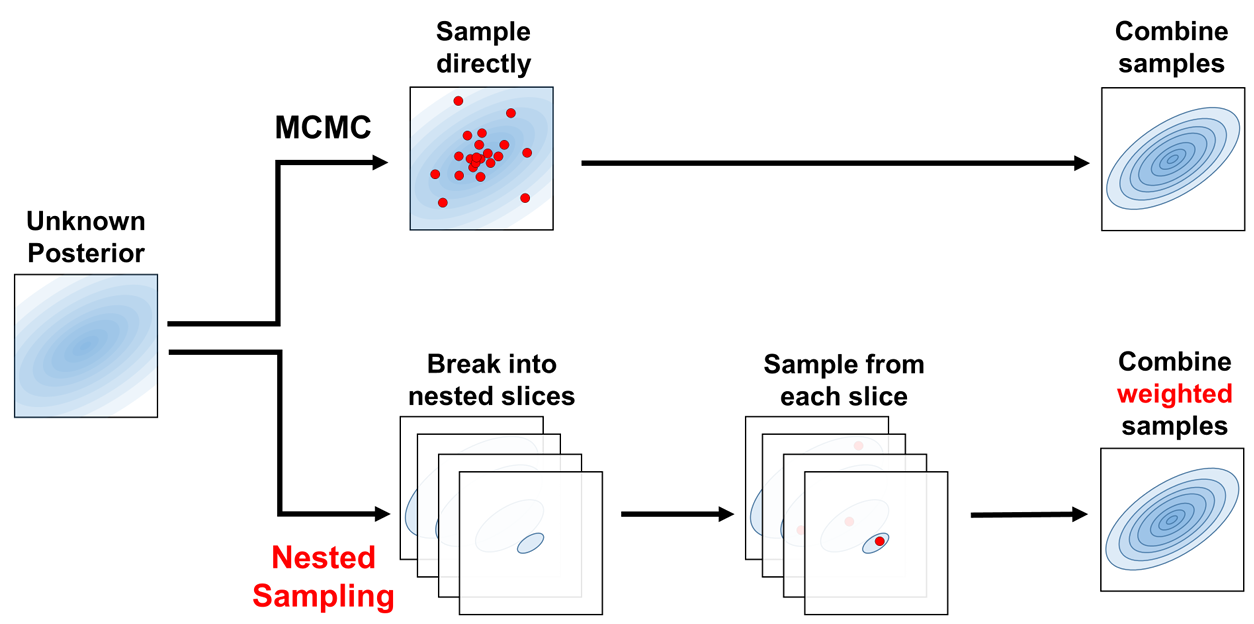
\includegraphics[width=0.73\linewidth]{Figures/MCMC_vs_nestedsampling.png}
    \caption{Schematic comparison of the two main stochastic sampling strategies. MCMC draws samples directly from the posterior via a random walk, combining them to reconstruct the distribution. Nested sampling instead decomposes the posterior into nested likelihood slices, samples from each slice independently, and combines the weighted samples to recover the posterior and compute the evidence $\mathcal{Z}$. Source: \cite{MCMC_vs_NS}.}
    \label{fig:MCMC_vs_nested}
\end{figure}

The output of both methods is a set of posterior samples 
$\{\boldsymbol{\theta}_k\}$ drawn from $p(\boldsymbol{\theta}|d,\mathcal{M})$, such that the density of samples in any region of parameter space is proportional to the posterior probability there. These samples can then be used to compute expectation values of any quantity of interest, to construct marginalized one- and two-dimensional 
posterior distributions for individual parameters, and to report credible intervals (the Bayesian analog of confidence intervals).

\paragraph{Markov Chain Monte Carlo.}
\label{MCMC}

MCMC methods construct a random walk through parameter space whose stationary distribution is the target posterior, as shown in Fig.~\ref{fig:MCMC_walk}. The most widely used variant is the Metropolis-Hastings algorithm, which proceeds as follows: starting from an initial point $\boldsymbol{\theta}_0$ (often drawn from the prior), at each iteration $t$ a new point $\boldsymbol{\theta}'$ is proposed from a proposal distribution $q(\boldsymbol{\theta}'|\boldsymbol{\theta}_t)$ (a common choice for $q$ is a Gaussian distribution with mean $\boldsymbol{\theta}_t$ and some fixed covariance matrix), and accepted with probability
\begin{equation}
    A = \min\!\left(1,\,
    \frac{p(\boldsymbol{\theta}'|d)\,
          q(\boldsymbol{\theta}_t|\boldsymbol{\theta}')}
         {p(\boldsymbol{\theta}_t|d)\,
          q(\boldsymbol{\theta}'|\boldsymbol{\theta}_t)}
    \right).
    \label{eq:MH}
\end{equation}
If $A \geq 1$ the proposal is always accepted; otherwise it is accepted with probability $A$. When the proposal distribution $q$ is symmetric, i.e.\ $q(\boldsymbol{\theta}'|\boldsymbol{\theta}_t) = q(\boldsymbol{\theta}_t|\boldsymbol{\theta}')$, the ratio of proposals cancels and $A$ reduces to the simple likelihood ratio $p(\boldsymbol{\theta}'|d)/p(\boldsymbol{\theta}_t|d)$. This acceptance rule ensures detailed balance and guarantees that the chain converges to the correct stationary distribution. By recording the position of the chain at each accepted step, one accumulates draws from the posterior.

\begin{figure}[h!]
    \centering
    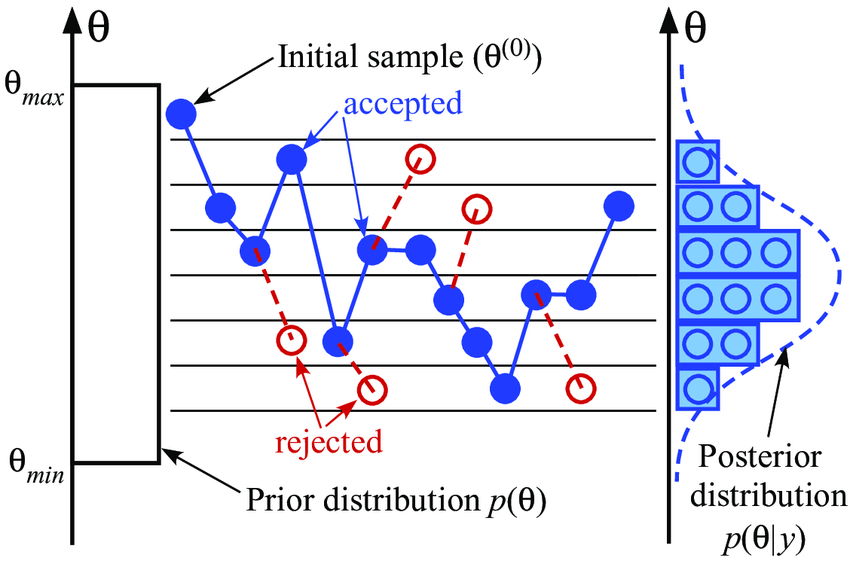
\includegraphics[width=0.61\linewidth]{Figures/MCMC_image}
    \caption{Illustration of the Metropolis-Hastings random walk in parameter space. Starting from initial samples drawn from the prior $\pi(\boldsymbol{\theta})$, walkers explore the parameter space following the acceptance criterion \eqref{eq:MH}, progressively converging toward the high-probability region of the posterior $p(\boldsymbol{\theta}|y)$. Source: \cite{image_MCMC}.}
    \label{fig:MCMC_walk}
\end{figure}

Several practical considerations arise. The early phase of the chain (the burn-in) is strongly dependent on the starting point and must be discarded before the chain has reached its stationary distribution. Successive samples within a chain are autocorrelated, so the chain must be thinned by retaining only samples separated by the autocorrelation length to obtain approximately independent draws. Finally, MCMC walkers can become trapped in a single mode of a multimodal posterior, a common situation in GW PE, where the sky position degeneracy produces two nearly symmetric modes. Parallel tempering mitigates 
this by running multiple chains at different temperatures 
(i.e., with artificially flattened posteriors) that periodically exchange states, allowing the cold chain to escape local maxima by borrowing proposals from hotter, more diffuse chains \cite{likelihood_formula}.

\paragraph{Nested sampling.}
\label{nested_sampling}

Nested sampling is an algorithm designed primarily to compute the evidence $\mathcal{Z}$ directly, with posterior samples produced as a byproduct. It is particularly well-suited to GW PE because it handles multimodal posteriors naturally and provides the evidence required for model comparison via the Bayes factor \eqref{eq:bayes_factor}. 

The algorithm proceeds as follows. A fixed number $N_\text{live}$ of live points are drawn uniformly from the prior. At each iteration, the live point with the lowest likelihood $\mathcal{L}_\mathrm{min}$ is removed and replaced by a new point drawn from the prior subject to the constraint $\mathcal{L} > \mathcal{L}_\mathrm{min}$, progressively shrinking the prior volume explored. The discarded point contributes to the evidence integral via the trapezoid rule,
\begin{equation}
    \mathcal{Z} \approx \sum_i \mathcal{L}_i\, w_i,
    \qquad
    w_i = X_{i-1} - X_i,
\end{equation}
where $X_i$ is the fraction of the prior volume enclosed by the $i$-th likelihood contour, estimated statistically from the number of live points. The algorithm terminates when the fractional contribution of the remaining prior volume to $\mathcal{Z}$ falls below a predefined threshold. Posterior samples are obtained by reweighting the discarded points by $\mathcal{L}_i w_i / \mathcal{Z}$. The geometric interpretation of the algorithm is shown in Fig.~\ref{fig:nested_sampling}.

\begin{figure}[h!]
    \centering
    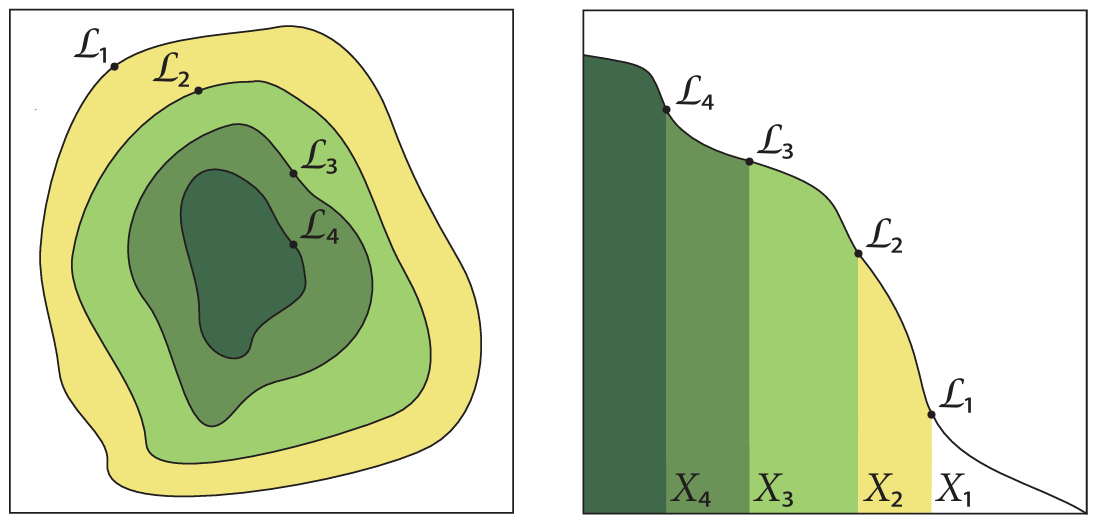
\includegraphics[width=0.63\linewidth]{Figures/Nested_sampling.png}
    \caption{Geometric interpretation of nested sampling. Left: iso-likelihood contours in parameter space, with the discarded live points $\mathcal{L}_1 > \mathcal{L}_2 > \mathcal{L}_3 > \mathcal{L}_4$ marking successive likelihood shells. Right: the corresponding one-dimensional mapping $\mathcal{L}(X)$ as a function of the enclosed prior volume $X$, where the evidence $\mathcal{Z}$ is approximated as the area under the curve via the trapezoid rule. Source: \cite{nestedsampling}.}
    \label{fig:nested_sampling}
\end{figure}

The main algorithmic challenge is drawing new live points 
efficiently from the likelihood-constrained prior. The most 
widely used implementations in GW astronomy are 
\textsc{MultiNest} \cite{MULTINEST}, which approximates the 
iso-likelihood contour with a set of ellipsoids that can be 
sampled exactly, and \textsc{Dynesty} \cite{MCMC_vs_NS}, which uses dynamic live-point allocation to concentrate computational effort where the posterior has the most support. Both are accessible through the \textsc{Bilby} \cite{BILBY} inference library, which provides a modular Python interface for CBC PE and is used in this work.


\vspace{0.5cm}


In summary, this chapter has established the theoretical and experimental foundations of GW astronomy. Beginning from the linearized EFE, we derived the existence of GWs as propagating spacetime perturbations, characterized their two polarization states, and quantified their effect on test masses through the geodesic deviation equation. We then surveyed the main astrophysical source classes and described the detection principle underlying current interferometric observatories, from the antenna pattern functions and noise budget to the global detector network. The chapter closed with the Bayesian PE framework (matched filtering, waveform models, and stochastic sampling) that allows us to extract source properties from detected signals. These tools constitute the methodological backbone of the analysis presented in the following chapters.

\newpage
\chapter{Gravitational lensing of gravitational waves}
\label{ch:lensing}


Having established the theoretical and observational foundations of GW astronomy in the preceding chapter, we now turn to a phenomenon that lies at the heart of this thesis: the gravitational lensing of GWs. We begin with the basics of gravitational lensing and its particular features in the GW context (\S\ref{sec:lensing_intro}), before developing the geometric optics formalism that governs strong 
lensing (\S\ref{sec:geometric_optics}). We then characterize the signatures that strong lensing imprints on GW signals, including the amplification factor, image classification, the Morse phase, and their effect on the observed strain and inferred source parameters (\S\ref{sec:strong_lensing}). The chapter closes with a discussion of how the joint analysis of lensed image pairs can be exploited to improve sky localization (\S\ref{sec:sky_localization_lensing}), 
motivating the methodology developed in the subsequent chapters.

\section{Gravitational lensing}
\label{sec:lensing_intro}

Gravitational lensing is a direct consequence of GR: massive objects curve spacetime, and any particle following a geodesic (including massless ones such as photons or GWs) will have its trajectory deflected \cite{EM_lensing,GW_lensing_original, Lensing_phase_effects}. The phenomenon was confirmed observationally by Eddington during the solar eclipse of 1919, when the apparent positions of stars near the Sun were displaced by exactly the amount predicted by 
GR \cite{Eddingtonsexpedition}. Since then, gravitational lensing has become one of the most powerful tools in observational astrophysics, providing information about the mass distribution of the Universe independently of its luminous content \cite{Lensing_in_astronomy}.

When a GW propagates from its source to a detector, massive 
structures along the line of sight act as gravitational lenses (galaxies, galaxy clusters,
and other compact objects). Depending on the geometry and lens mass, three regimes are distinguished \cite{lensing_regimes}: strong lensing, caused by galaxies or galaxy clusters, produces multiple images of the same source arriving at different times and with different amplitudes; microlensing, caused by compact objects, produces overlapping images whose interference can modulate the observed strain; and weak lensing, due to large-scale structure, induces small coherent distortions. Figure~\ref{fig:diagram_GW_lensing_Regimes} illustrates the general picture of GW lensing, including both strong-lensing and microlensing effects. This work focuses exclusively on the strong lensing regime.

\newpage
\begin{figure}[h!]
    \centering
    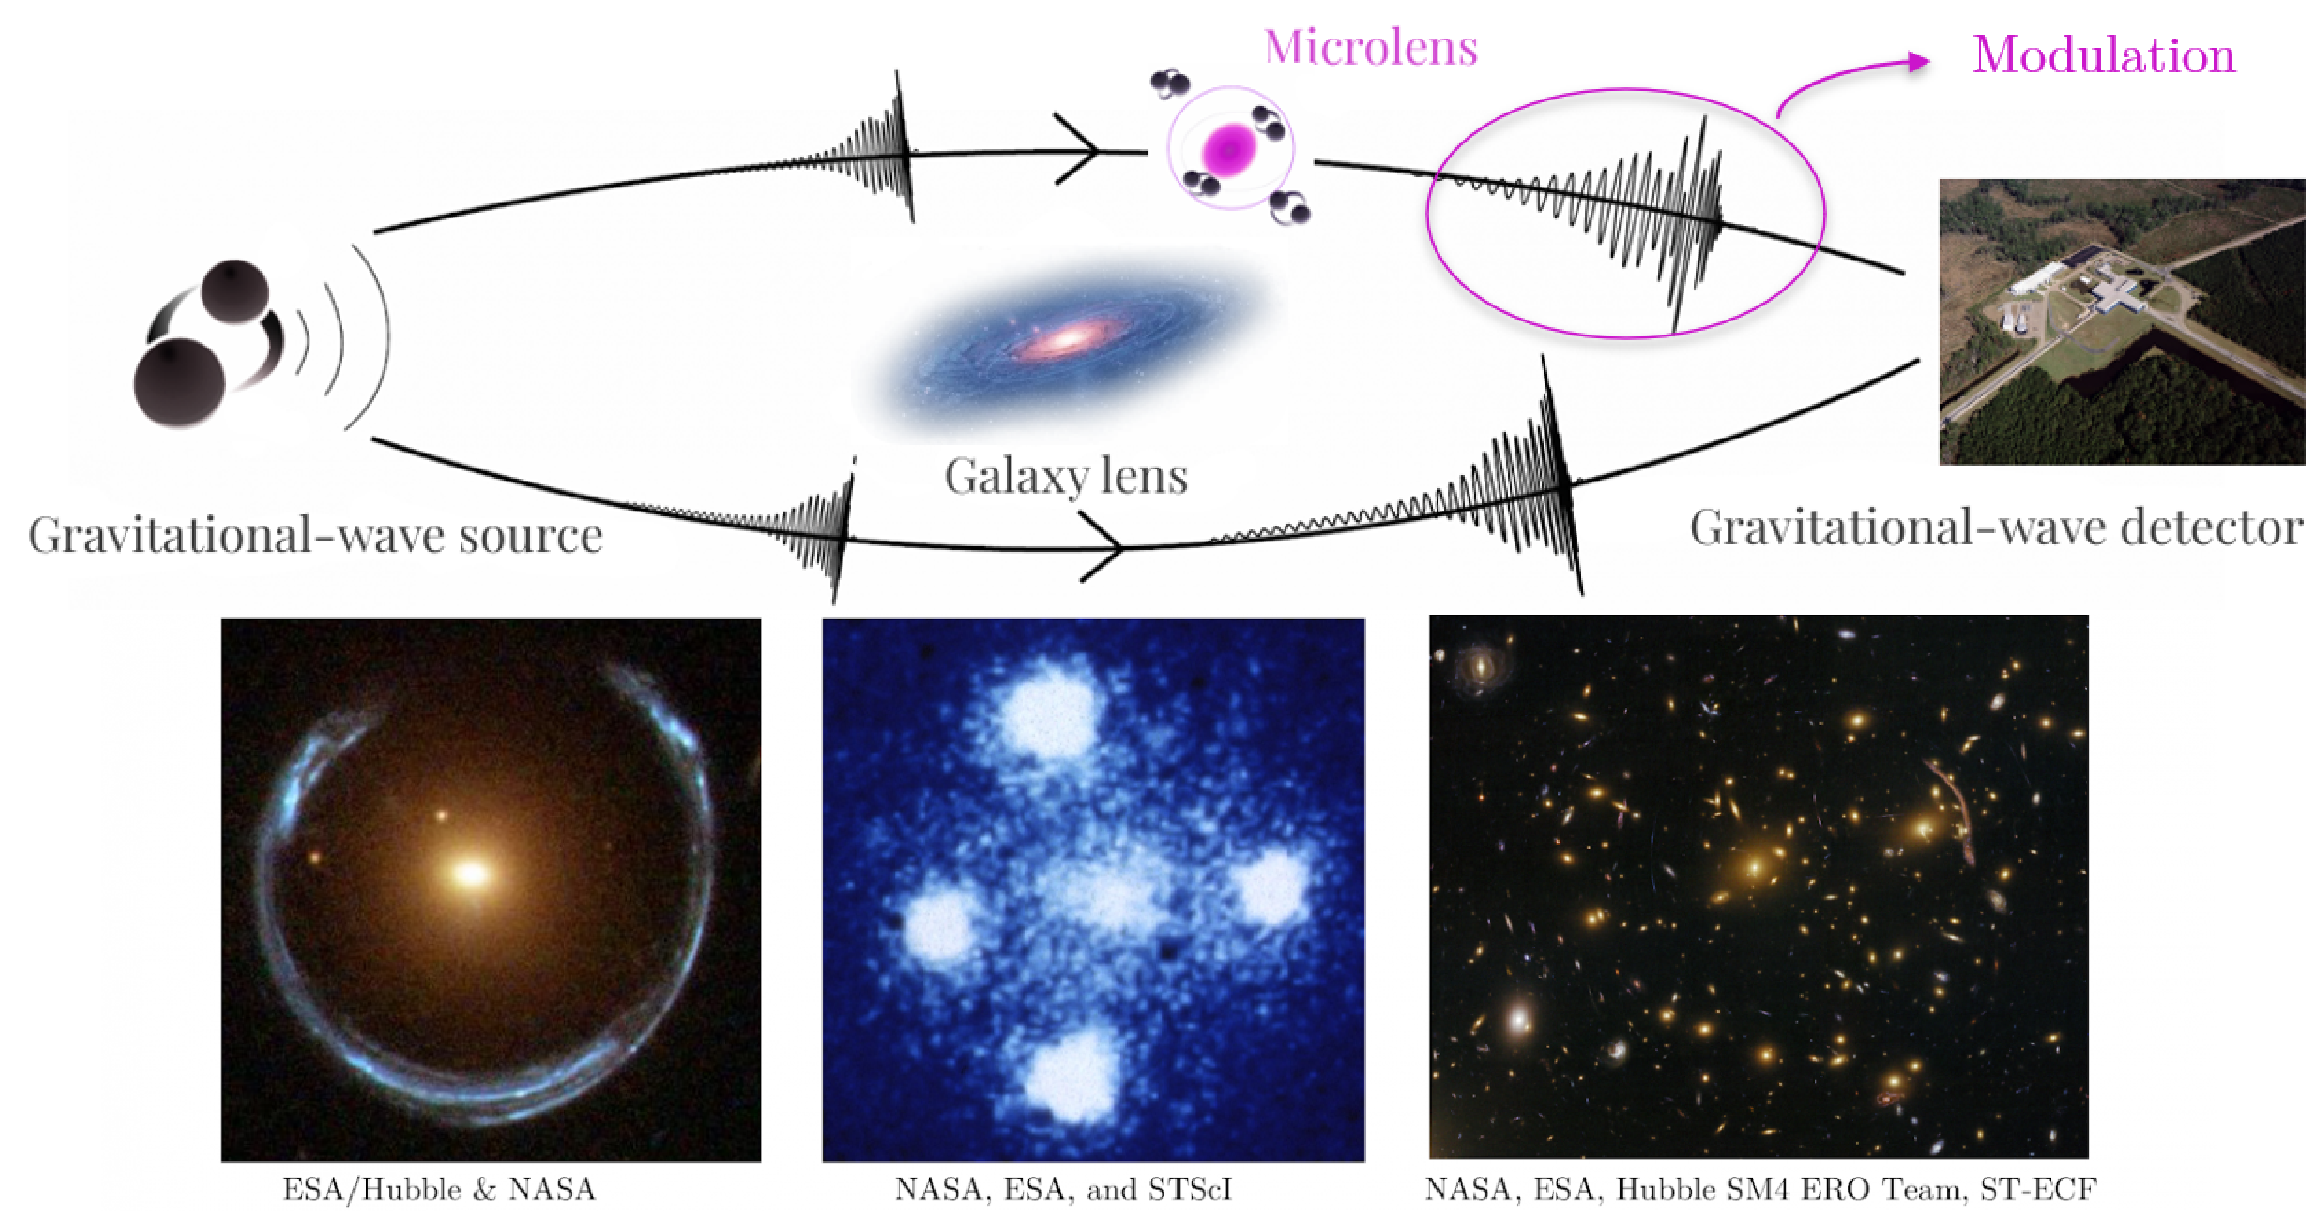
\includegraphics[width=0.86\linewidth]{Figures/Millilens.pdf}
    \caption{Schematic representation of GW lensing. A galaxy acting as a macrolens can produce multiple images of the same GW signal, arriving at the detector with different magnifications and time delays. Compact objects embedded within the lens galaxy (microlenses) can further perturb these images, introducing additional amplification, interference, and diffraction effects. The images shown at the bottom illustrate examples of strong gravitational lensing observed in electromagnetic astronomy. Original illustration based on sources: \cite{LIGO_lensing_image, Figure_micro_strong_lensing}.}
    \label{fig:diagram_GW_lensing_Regimes}
\end{figure}



\subsection{Differences between electromagnetic and gravitational 
wave lensing}

Although the deflection of EM waves and GWs follows the same 
underlying physics, several important differences arise from their distinct nature. The most fundamental concerns the wavelength regime. GWs detectable by ground-based interferometers have wavelengths ranging from roughly 10\,km to 1\,Mm, far larger than EM wavelengths. The relevant parameter is the ratio $\lambda_\mathrm{GW}/\lambda_E$, where $\lambda_E$ is the Einstein radius of the lens (see $\S$\ref{???}). When $\lambda_\mathrm{GW} \ll \lambda_E$, the geometric optics approximation is valid. When $\lambda_\mathrm{GW} \gtrsim \lambda_E$ (which can occur for low-mass lenses) wave optics must be used and diffraction produces frequency-dependent modulations of the waveform with no EM analog \cite{Wave_optics_GW}. Figure~\ref{fig:wave_optics_regime} illustrates the lens-mass scales associated with these two regimes. For the galaxy-scale lenses relevant to this work, $\lambda_E \sim \mathcal{O}(\mathrm{kpc})$, placing the problem firmly in the geometric optics regime.

A second difference is coherence. GWs are coherent waves with a well-defined phase, so lensed images can interfere if their time delay is shorter than the signal duration (an effect absent in standard EM lensing). Finally, unlike EM signals, GWs are not absorbed or dispersed by the intergalactic medium, encoding clean information about the source and lensing potential.


\begin{figure}[h!]
    \centering
    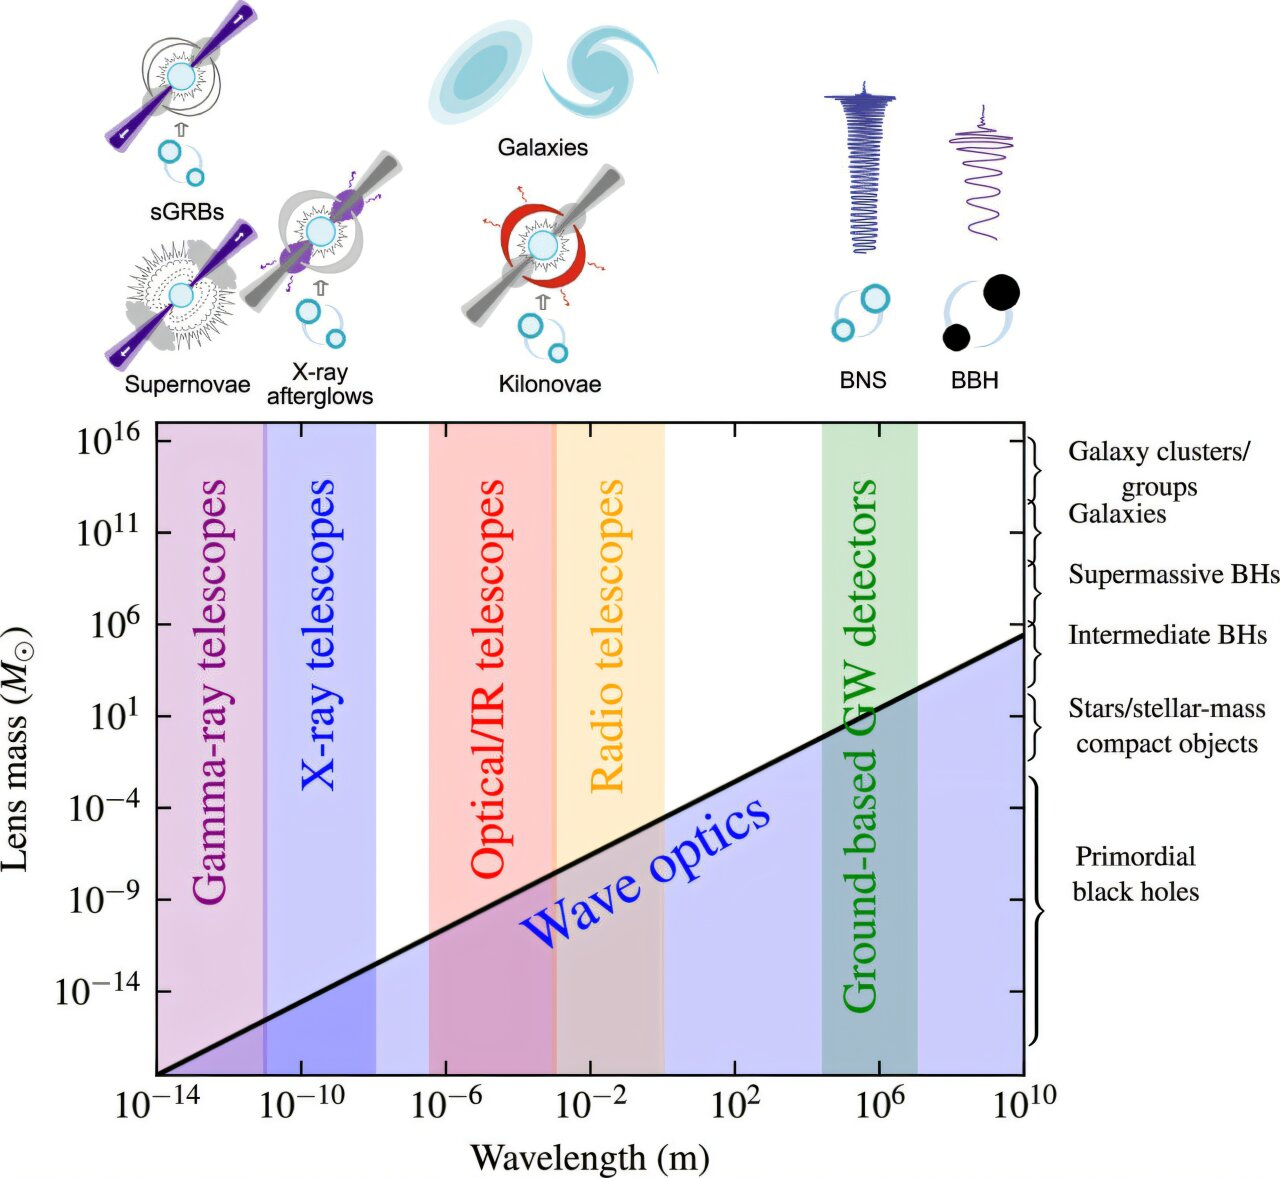
\includegraphics[width=0.63\linewidth]{Figures/wave_optics_lensing.jpg}
    \caption{Illustration of the lens-mass scales relevant for gravitationally lensed signals. Depending on the relation between the radiation wavelength and the characteristic scale of the lensing potential, lensing occurs in either the geometric optics or wave optics regime. While geometric optics describes distinct propagation paths, wave optics accounts for diffraction and interference effects. Due to their long wavelengths, GW can exhibit wave-optics effects for relatively low lens masses. Source: \cite{multi_messenger_gravitational_lensing}.}
    \label{fig:wave_optics_regime}
\end{figure}



\subsection{Relevance for gravitational wave astronomy}

No confirmed detection of gravitational lensing of GWs has been reported despite dedicated searches in GWTC-1 through GWTC-4 \cite{GWTC4_introduction}. As detector sensitivities improve, detection is expected to become feasible within the next observing runs, with predictions suggesting more than one strongly lensed event per year at design sensitivity \cite{Hannuksela_2019}.

Such detections would open a rich set of applications: measuring the Hubble constant via lensing time delays combined with GW standard sirens \cite{Schutz1986, hubble_constant_lensing}, probing dark matter distributions in lens galaxies \cite{jana2024probingnaturedarkmatter}, and testing GR by comparing the propagation speed of GWs and light through the same lensing potential \cite{test_GR_lensing}. Lensing also biases the apparent properties of detected sources (a magnified image appears closer and more massive than it truly is) making the identification of lensed events important for controlling systematics in population studies \cite{population_lensing}.

In addition, multiple images of the same source provide repeated observations that can be combined to improve PE and sky localization \cite{hubble_constant_lensing, Chen_2025}. This last application is the central motivation of the present work: by performing a joint Bayesian analysis of two strongly lensed images of the same BBH merger, we investigate how the sky localization of the source can be dramatically improved compared to the analysis of a single image.


\section{Geometric optics regime}
\label{sec:geometric_optics}



blasnalsnl

\subsection{The lens equation}
\subsubsection{Deflection angle}
\subsubsection{Thin lens approximation}
\subsection{Einstein radius and image formation}
\subsection{Magnification and time delay}
\subsubsection{Geometric and Shapiro time delay}
\subsubsection{Magnification}
\subsection{Lens models}
\subsubsection{Point mass lens}
\subsubsection{Singular isothermal sphere}

\section{Strong lensing of gravitational waves}
\label{sec:strong_lensing}

\section{Strong lensing of gravitational waves}
\label{sec:strong_lensing}

\subsection{Strong vs weak lensing}

\subsection{Amplification factor in the geometric optics limit}
% Aquí introduces F(f) = sqrt(mu) exp(...)
% Es el puente entre geometric optics y la señal

\subsection{Image types and Morse phase}
\subsubsection{Type I, II and III images}
\subsubsection{Effect of the Morse phase on the waveform}

\subsection{Lensed gravitational wave strain}
% Aquí metes h_L = F * h, que es consecuencia directa del amplification factor
% Ya no necesitas una sección separada

\subsection{Apparent vs intrinsic parameters}
\subsubsection{Redshifted masses}
\subsubsection{Magnification bias on luminosity distance}

\subsection{Lensing observables}
\subsubsection{Magnification ratio}
\subsubsection{Time delay between images}


\section{Sky localization of lensed image pairs}
\label{sec:sky_localization_lensing}

\subsection{Sky localization with a single GW image}
\subsection{Joint parameter estimation of lensed pairs}
\subsection{Lensing hypothesis testing}
\subsubsection{Lensing vs non-lensing Bayes factor}
\subsubsection{Overlap integral}

................





**Differences between EM and GW lensing**
- Las GWs son coherentes (tienen fase), las ondas EM normalmente no → el lensing produce interferencia en GWs
- Las GWs tienen dos polarizaciones → el lensing las afecta de forma específica
- No hay absorción ni dispersión en el medio interestelar para GWs
- La fuente de GW es puntual y bien modelada → más fácil detectar anomalías

**Relevance for GW astronomy**
Por qué importa para tu trabajo: las GWs lensadas pueden confundirse con eventos independientes, pueden usarse para cosmología (tiempo de retardo  $H_0$), y el lensing fuerte produce múltiples imágenes que es exactamente lo que estudias.

---

**Deflection angle**
Derivación del ángulo de deflexión de un rayo que pasa a distancia $\xi$ de una masa $M$: $\hat{\alpha} = 4GM/c^2\xi$. Comparar con el resultado newtoniano (factor 2).

**Thin lens approximation**
La deflexión ocurre en un plano — el plano de la lente. Justificación: la lente es mucho más delgada que las distancias fuente-lente y lente-observador. Esto simplifica enormemente la geometría.

**The lens equation**
La ecuación que relaciona la posición de la fuente $\beta$, la posición de la imagen $\theta$ y el ángulo de deflexión $\hat{\alpha}$:
$$\boldsymbol{\beta} = \boldsymbol{\theta} - \boldsymbol{\alpha}(\boldsymbol{\theta})$$
Esto es el punto de partida para todo lo que sigue.

**Einstein radius and image formation**
El radio de Einstein $\theta_E$ como escala natural del lensing. Cuándo se forman múltiples imágenes (cuando la fuente está dentro del radio de Einstein). El anillo de Einstein como caso especial de alineación perfecta.

**Geometric and Shapiro time delay**
El tiempo de retardo entre imágenes tiene dos contribuciones: geométrica (caminos de distinta longitud) y de Shapiro (la luz se ralentiza en el pozo gravitacional). La combinación da el tiempo de retardo total $\Delta t$ entre imágenes — clave para tu análisis.

**Magnification**
El lensing conserva la brillancia superficial pero distorsiona el área → magnificación $\mu$. Para GWs, una imagen magnificada tiene mayor SNR. El ratio de magnificación entre las dos imágenes $\mu_1/\mu_2$ es un parámetro observable.

**Point mass lens**
El modelo más simple: toda la masa concentrada en un punto. Solución analítica exacta. Produce siempre dos imágenes. Es el modelo que usa LER/Hanabi → justifica por qué lo introduces.

**Singular isothermal sphere (SIS)**
Modelo de galaxia más realista: perfil de densidad $\rho \propto r^{-2}$. Puede producir dos imágenes con igual magnificación. Mencionarlo brevemente como alternativa al punto masa.

---

**Strong vs weak lensing**
Definición operativa: strong lensing cuando $\theta_E \gtrsim$ separación angular de la fuente → múltiples imágenes resolvibles. Weak lensing: solo distorsión suave, no hay imágenes múltiples. Para GWs no se "ven" las imágenes separadas pero sí se detectan como eventos distintos → por eso el strong lensing es detectable.

**Type I, II and III images**
Clasificación según la topología del tiempo de retardo: mínimo (Type I), silla de montura (Type II), máximo (Type III). Cada tipo tiene una signatura de fase diferente.

**Effect of the Morse phase on the waveform**
El tipo de imagen determina una fase adicional en la forma de onda: Type I → $n=0$, Type II → $n=1/2$ (transformada de Hilbert), Type III → $n=1$. Esto es crucial porque cambia la morfología de la señal detectada y puede confundirse con un cambio en los parámetros de la fuente.

**Amplification factor in the geometric optics limit**
La forma compacta $F_j = \sqrt{\mu_j}\exp(-2\pi i f t_j \pm i\pi n_j)$ que multiplica la señal sin lensing. Es exactamente lo que implementa Hanabi → conecta directamente con tu metodología.

---

**Modification of the GW strain**
La señal lensada es $\tilde{h}_L(f) = F(f)\,\tilde{h}(f)$ donde $F$ es el factor de amplificación. En geometric optics cada imagen es una copia de la señal original con distinta amplitud, fase y tiempo de llegada.

**Redshifted masses**
Una imagen más magnificada parece más cercana → masa aparente diferente de la masa intrínseca. En particular $m^\mathrm{det} = (1+z_L)m^\mathrm{src}$. Si no se sabe que hay lensing se infieren masas incorrectas — relevante para interpretar tus posteriors.

**Magnification bias on luminosity distance**
La magnificación $\mu$ cambia la distancia luminosa aparente: $D_L^\mathrm{app} = D_L/\sqrt{\mu}$. Una imagen magnificada parece más cercana. Esto afecta directamente a la sky localization porque $D_L$ y $(\alpha,\delta)$ están correlacionados.

**Magnification ratio, time delay, Morse phase difference**
Los tres parámetros observables que caracterizan un par de imágenes lensadas. Son los parámetros de lensing que LER inyecta y que Bilby recupera. Introducirlos aquí los justifica antes de usarlos en resultados.

---

**Sky localization with a single GW image**
Recordar del capítulo anterior: una sola imagen da una región anular en el cielo. La distancia y la inclinación están degeneradas. Sin EM counterpart la localización es pobre.

**Joint parameter estimation of lensed pairs**
Con dos imágenes que comparten los mismos parámetros intrínsecos ($m_1, m_2, \chi_i$) pero tienen diferentes parámetros extrínsecos aparentes, el análisis conjunto rompe degeneraciones. El joint posterior en $(\alpha,\delta)$ es la intersección de las dos regiones individuales → mucho más pequeña. Esta es la motivación central de tu proyecto.

**Lensing vs non-lensing Bayes factor**
El formalismo ya introducido en §\ref{sec:bayes_factor} aplicado al caso específico: $\mathcal{M}_L$ (los dos eventos son imágenes del mismo BBH) vs $\mathcal{M}_{NL}$ (son dos BBH independientes). El Bayes factor cuantifica qué hipótesis favorecen los datos.

**Overlap integral**
Métrica alternativa de consistencia: mide el solapamiento entre los posteriors de las dos imágenes en los parámetros intrínsecos compartidos. Si las dos imágenes son del mismo evento, los posteriors en $m_1, m_2, \chi_i$ deben ser compatibles.
---------------


................
This overview of gravitational lensing of GW marks the conclusion of the first part of the thesis. Now, we have all the necessary tools to describe the results obtained in this study.

ARREGLAR PART SUMMARY


\part{Original results}
 \vspace{4cm}
 At this point, we have all the necessary tools to describe the results
 of this thesis.
 The first one, reported in Chapter 5, is a gravitational wave-like propa
gation on the top of an acoustic metric. Notably, in the past only static
 solutions of GR were designed in analogue models. Here,
 we present a system where analogue gravitational waves propagate sat
isfying Einstein’s equations.
 The second result, in Chapter 6, consists in designing a system in which
 an acoustic horizon is excited by a gravitational wave-like perturbation.
 To this purpose, we choose a cylindrical acoustic black hole, where we
 introduce an appropriate extension in the geometry of the previously
 found gravitational wave-like perturbation.


\newpage


\chapter{Simulation setup and implementation}
\label{Simulation_setup}

\section{Lensed BBH population with LER}
% Explicar qué es LER y para qué lo usas
% Parámetros: npool, event_type BBH, ifos L1 H1
% PSD: T2500310-v2_O5a_strain_psd (O5 design sensitivity)
% Waveform: IMRPhenomXPHM, spin precession
% Criterio de selección: 500 eventos con SNR >= 10 en ambas imágenes

\section{Injected parameter distributions}
% Plots de m1, m2 con crosses de los valores inyectados
% Distribución de masas, spins, distancias
% Histogram SNR de L1, H1 y joint para ambas imágenes
% Plots LER de los parámetros de lensing: time delay, magnification ratio


\chapter{Parameter estimation pipeline}
\label{Parameter_estimation_pipeline}

\section{Lensed waveform generation with Hanabi}
% Qué es Hanabi y cómo genera señales lensadas
% strongly_lensed_BBH_waveform con IMRPhenomXPNR
% image_type (Morse phase), relative_magnification
% Cómo se conecta LER → Hanabi → Bilby

\section{Bilby configuration and joint analysis}
% Estructura del ini file: label, outdir, request-cpus=128
% Sampler: dynesty, nlive=1000, naccept=60, acceptance-walk
% n-triggers=2, trigger-ini-files (image1 + image2)
% common-parameters: chirp_mass, mass_ratio, spins, ra, dec, psi, phase
% lensing-prior-dict: relative_magnification, image_type DiscreteUniform
% Por qué se hace análisis conjunto (joint) y no individual

\section{Automation and infrastructure}
% Cómo automatizas la creación de ini files para 500 inyecciones
% Submission a Picasso con SLURM
% Gestión de outputs y JSON results

\section{Residuals and parameter recovery}
% Violin plots  
% residuals (parámetros recuperados vs inyectados)
% Scatter plots
\subsection{SNR comparison}
% Comparación entre el SNR calculado por LER y el recuperado por Bilby
% Validación del setup}

\chapter{Sky localization}
\label{Skyloc}

\section{Sky map generation}
% ligo-skymap-from-samples: genera el skymap.fits a partir 
% de los posterior samples de Bilby
% --disable-distance-map, --trials 1
% Se hace para cada imagen individual y para el joint

\section{Sky area and constellation analysis}
% ligo-skymap-stats: extrae el área al 90% de credibilidad
% ligo-skymap-constellations: asigna la región a constelaciones
% Plot SNR vs sky area 90%
% Plot SNR vs constellation

\section{Comparison between single image and joint analysis}
% PDF y CDF del sky area comparando:
%   - imagen individual (la mejor, mayor SNR)
%   - análisis joint de las dos imágenes
% Mejora cuantitativa en la localización



FUTURE WOOOORKKK


To summarize, in this chapter we have developed the description of an acoustic
 cylindrical black hole perturbed by a gravitational wave-like perturbation. This
 perturbation is introduced as the cylindrical extension of the analogue gravitational
 wave found in Chapter 5. After having illustrated the designed physical system,
 we have studied how the acoustic horizon is perturbed by the impinging analogue
 gravitational wave, computing also its generators. This analogue model is important
 since it allows to study how an acoustic horizon responds to a gravitational wave-like
 perturbation.

\chapter{Conclusions}
\label{Conclusions}

Future work

 In this thesis work we have obtained two original results:
 1. ...
 2. ...
 These results are shown in Chapter ? and in Chapter ?, respectively. In particular,
 in Section ? we have shown... . Instead, in Sections ?
 and ? we have studied... 


 mencionar aixó: Several idealizations in the pipeline described above should be kept in mind when interpreting the results of this thesis. The noise realizations added to each injection are stationary and Gaussian (\texttt{gaussian-noise=True}), so none of the non-Gaussian transients \ref{sec:noise} (glitches) that affect real LIGO data are present; a real search would need to contend with this additional source of PE bias and false coincidences. The same projected O5a PSD is used for both H1 and L1, whereas the two real detectors have distinct, time-varying noise budgets; this symmetry is not expected to qualitatively change the sky localization results, which depend primarily on the relative antenna pattern and time delay between the two sites, but it does idealize the relative sensitivity assumed for each detector. Finally, the analysis assumes perfect detector calibration and does not marginalize over calibration uncertainty, an additional source of systematic error present in real LVK analyses that is not modelled here.


\printbibliography[heading=bibintoc, title={Bibliography}]

\appendix


\renewcommand{\thechapter}{A} 
\chapter{Parameters of Compact Binary Coalescences}
\label{Parameters_CBC_appendix}

This appendix provides a reference summary of the parameters used to describe a CBC system with quasi-circular orbits, following the conventions of \cite{likelihood_formula, GWTC4_introduction}. The parameters are grouped into mass, spin, tidal, and extrinsic categories; those employed in the injections and PE analyses of this work are indicated with $\star$.

\renewcommand{\arraystretch}{1.3}

{
\setlength{\LTleft}{0pt plus 1fill}
\setlength{\LTright}{0pt plus 1fill}
\begin{longtable}{lcp{9cm}}

\caption{Parameters describing a CBC system with quasi-circular orbits \cite{likelihood_formula, GWTC4_introduction}. Parameters used in this work are indicated with $\star$.}
\label{tab:CBC_parameters} \\

\hline\hline
\multicolumn{1}{c}{Parameter name} &
\multicolumn{1}{c}{Symbol} &
\multicolumn{1}{c}{Definition [Dimensions]} \\
\midrule
\endfirsthead

\multicolumn{3}{c}%
{{\tablename\ \thetable\ \textit{(continued)}}} \\

\hline\hline
\multicolumn{1}{c}{Parameter name} &
\multicolumn{1}{c}{Symbol} &
\multicolumn{1}{c}{Definition [Dimensions]} \\
\midrule
\endhead

\hline
\addlinespace[4pt]
\multicolumn{3}{c}{{\textit{Continued on next page}}} \\
\endfoot

\bottomrule
\endlastfoot

%------------------------------------------------
\addlinespace[5pt]
\multicolumn{3}{l}{\textit{\textbf{Mass parameters}}} \\
\hline
\addlinespace[5pt]

\, Primary/secondary mass & $m_1^\star,\,m_2^\star$ &
Mass of the more (less) massive component, $m_1\geq m_2$ $[M_\odot]$ \\

\, Chirp mass & $\mathcal{M}$ &
$\mathcal{M}=\eta^{3/5}M$ $[M_\odot]$ \\

\, Total mass & $M$ &
$M=m_1+m_2$ $[M_\odot]$ \\

\, Final mass & $M_f$ &
Mass of the remnant $[M_\odot]$ \\

\, Mass ratio & $q$ &
$q=m_2/m_1\leq 1$ [dimensionless] \\

\, Symmetric mass ratio & $\eta$ &
$\eta=m_1m_2/M^2\leq 1/4$ [dimensionless] \\

\, Radiated energy & $E_\mathrm{rad}$ &
$E_\mathrm{rad}=(M-M_f)c^2$ [energy] \\

%------------------------------------------------
\addlinespace[5pt]
\multicolumn{3}{l}{\textit{\textbf{Spin parameters}}} \\
\hline
\addlinespace[5pt]

\, Primary/secondary spin vectors & $\mathbf{S}_1,\,\mathbf{S}_2$ &
Spin angular momentum of the primary/secondary [ang. mom.] \\

\, Dimensionless spin magnitudes & $\chi_1^\star,\,\chi_2^\star$ &
$\chi_{1,2}=c|\mathbf{S}_{1,2}|/(Gm_{1,2}^2)\leq 1$ [dimensionless] \\

\, Remnant spin magnitude & $\chi_f$ &
$\chi_f=cS_f/(GM_f^2)\leq 1$  where $S_f$ is the magnitude of the remnant's spin
angular momentum [dimensionless] \\

\, Orbital ang. momentum & $\mathbf{L}$ &
Instantaneous orbital angular momentum about the center of mass [ang. mom.] \\

\, Total ang. momentum & $\mathbf{J}$ &
$\mathbf{J}=\mathbf{L}+\mathbf{S}_1+\mathbf{S}_2$ [ang. mom.] \\

\, Primary/secondary tilt angles & $\theta_1^\star,\,\theta_2^\star$ &
Angle between $\mathbf{S}_{1,2}$ and $\mathbf{L}$ [angle] \\

\, Spin azimuthal difference & $\phi_{12}^\star$ &
Angle between $\mathbf{L}\times(\mathbf{S}_1\times\mathbf{L})$ and $\mathbf{L}\times(\mathbf{S}_2\times\mathbf{L})$ [angle] \\

\, Effective inspiral spin & $\chi_\mathrm{eff}$ &
$(m_1\chi_{1z}+m_2\chi_{2z})/M$ [dimensionless] \\

\, Effective precession spin & $\chi_p$ &
Avg.\ over precession cycles \cite{effective_precession_spin} [dimensionless] \\

%------------------------------------------------
\multicolumn{3}{l}{\textit{\textbf{Tidal parameters}}} \\
\hline
\addlinespace[5pt]

\, Tidal deformabilities & $\Lambda_1,\,\Lambda_2$ &
Dimensionless tidal deformability; $\Lambda_{1,2}=0$ for BHs [dimensionless] \\

\, Effective tidal deformability & $\tilde{\Lambda}$ &
Dominant tidal combination; $\tilde{\Lambda}=0$ for BBH [dimensionless] \\

%------------------------------------------------
\multicolumn{3}{l}{\textit{\textbf{Extrinsic parameters}}} \\
\hline
\addlinespace[5pt]

\, Luminosity distance & $D_L^\star$ &
Distance to the source [Mpc] \\

\, Redshift & $z$ &
Computable from $D_L$ assuming a cosmological model [dimensionless] \\

\, Source inclination & $\theta_{JN}^\star$ &
Angle between $\mathbf{J}$ and line of sight $\mathbf{N}$ [angle] \\

\, Orbital inclination & $\iota$ &
Angle between $\mathbf{L}$ and $\mathbf{N}$ [angle] \\

\, Coalescence time & $t_c^\star$ &
GPS time at the geocenter [time] \\

\, Coalescence phase & $\phi_c^\star$ &
Orbital phase at coalescence [angle] \\

\, Right ascension & $\alpha^\star$ &
Celestial longitude [angle] \\

\, Declination & $\delta^\star$ &
Celestial latitude [angle] \\

\, Polarization angle & $\psi^\star$ &
Rotates polarizations in the plane orthogonal to propagation [angle] \\

\, Azimuthal spin angle & $\phi_{JL}^\star$ &
Angle between $\mathbf{J}$ and $\mathbf{L}$ projected on the sky plane [angle] \\
\end{longtable}
}



\renewcommand{\thechapter}{B} 
\chapter{Practical guide to HPC workflows}
\label{Reproducibility tutorial}

The motivation for including this appendix comes from the desire to make life easier for future students who will use the same tools, especially since many parts of this tutorial came with their fair share of headaches. It collects the day-to-day commands, configuration patterns, and troubleshooting notes accumulated while running the analyses of this thesis on two HPC clusters. It is not a repetition of the pipeline described in \S\ref{sec:automation_picasso}, but a practical reference for a student facing the same kind of environment for the first time. All pipeline-specific reproducibility details (configuration files, directory layout, job dependency logic) are documented in \S\ref{sec:automation_picasso} and Appendix~$\S$\ref{implementataion_pipeline}; the complete code is publicly available at \url{https://github.com/XxavierGarcia/TFM_reproducibility_material}.

\section{SSH access and aliases}

Both clusters are accessed via SSH (Secure Shell), a protocol that opens an encrypted terminal session on a remote machine: once connected, commands typed locally are executed directly on the cluster, as if sitting in front of it. On a Linux machine, an SSH client is available out of the box:

\begin{verbatim}
ssh username@picasso.scbi.uma.es
\end{verbatim}

(Users connecting from Windows Subsystem for Linux may need to append \texttt{-o KexAlgorithms=\allowbreak ecdh-sha2-nistp521} to this and every following \texttt{ssh}/\texttt{scp} command, since its older default OpenSSH client does not otherwise offer an algorithm accepted by Picasso's server; this flag is omitted from the rest of this tutorial.)

On CIT, the IGWN LDAS head nodes serve as the entry point (LIGO.ORG credentials required):

\begin{verbatim}
ssh username@ldas-grid.ligo.caltech.edu
\end{verbatim}

Typing these every time quickly becomes impractical. Two alternatives exist. The first is to define shell aliases in \texttt{\textasciitilde/.bashrc}:

\begin{verbatim}
alias picasso='ssh username@picasso.scbi.uma.es'
alias caltech='ssh username@ldas-grid.ligo.caltech.edu'
\end{verbatim}

Once these lines are added and the shell configuration is reloaded (\texttt{source \textasciitilde/.bashrc} or a new terminal), the full commands above are replaced by simply typing \texttt{picasso} or \texttt{caltech}.

The second, more robust option is to add entries to \texttt{\textasciitilde/.ssh/config}:

\begin{verbatim}
Host picasso
    HostName picasso.scbi.uma.es
    User username
    IdentityFile ~/.ssh/id_rsa
\end{verbatim}

With this configuration, \texttt{ssh picasso} and \texttt{scp picasso:path/file .} work directly.

\section{Remote editing with VS Code}

Editing files on the cluster through \texttt{nano} or \texttt{vim} works but is slow for larger scripts. VS Code's {Remote - SSH} extension provides a full graphical editor connected to the cluster filesystem:

\begin{enumerate}
  \item Install the \textit{Remote - SSH} extension from the VS Code marketplace.
  \item Open the command palette (\texttt{Ctrl+Shift+P}), type \textit{Remote-SSH: Connect to Host}, and select the host (or add a new one pointing to \texttt{picasso.scbi.uma.es}).
  \item Once connected, use \textit{File $\to$ Open Folder} to navigate to the working directory.
\end{enumerate}

This allows browsing the directory tree, viewing output figures directly, and editing configuration files without leaving the editor.

\section{Transferring files with \texttt{scp}}

\texttt{scp} (secure copy) transfers files between any two machines reachable via SSH. The basic syntax is \texttt{scp [options] source destination}, where either side can be \texttt{host:path}.

\begin{verbatim}
# Copy a single file from the local machine to the cluster
scp local_file.py username@picasso.scbi.uma.es:~/lenskyloc/

# Copy an entire directory (-r for recursive)
scp -r username@picasso.scbi.uma.es:~/lenskyloc/inj001/result/ .

# Transfer between two clusters (run from CIT)
scp -r username@picasso.scbi.uma.es:~/lenskyloc/pesummary_jsons .
\end{verbatim}

On CIT, the Jupyter interface (\url{https://jupyter.ligo.caltech.edu}) provides an alternative for downloading files: compress them first with \texttt{zip -r archive.zip directory/} and download the archive through the browser.

\section{Persistent terminal sessions with \texttt{screen}}

An SSH connection that drops (timeout, laptop closing, network change) kills any process running inside it. The \texttt{screen} utility creates a persistent terminal session on the cluster that survives disconnections:

\begin{verbatim}
screen -S analysis         # create a named session
# ... run any long command ...
# detach: Ctrl+a, then d
screen -ls                 # list active sessions
screen -r analysis         # reattach
exit                       # close the session permanently
\end{verbatim}

This is essential for interactive tasks that take more than a few minutes (monitoring logs, running quick post-processing scripts) but are not worth submitting as batch jobs.

\section{Conda environments}

Both clusters use \texttt{conda} environments to manage Python dependencies. On Picasso, the analysis environment was created and maintained manually:

\begin{verbatim}
conda create -n hanabi_bilby260 python=3.10
conda activate hanabi_bilby260
pip install bilby bilby_pipe hanabi lalsuite dynesty ...
\end{verbatim}

The activation line is included in every generated SLURM script, so each job runs in the correct environment automatically. On CIT, the \texttt{igwn} environment distributed via CVMFS is activated directly instead.

When the home directory quota on Picasso fills up (check with \texttt{quota}), the most effective remedy is to clear the conda cache, which accumulates downloaded packages and can grow to several gigabytes:

\begin{verbatim}
conda clean --all
\end{verbatim}

\section{SLURM: submitting and monitoring jobs on Picasso}

Picasso uses the SLURM workload manager. Jobs are submitted with \texttt{sbatch}, monitored with \texttt{squeue}, and cancelled with \texttt{scancel}:

\begin{verbatim}
sbatch job_script.sh           # submit a job
squeue -u username             # list your running/pending jobs
scancel JOB_ID                 # cancel one job
scancel --user username        # cancel all your jobs
\end{verbatim}

A typical SLURM header for a single-image PE job in this thesis (\S\ref{sec:bilby_config}) looks like:

\begin{verbatim}
#!/bin/bash
#SBATCH --job-name=lenskyloc_inj_001_img1
#SBATCH --cpus-per-task=128
#SBATCH --mem=110G
#SBATCH --time=48:00:00
#SBATCH --constraint=cal

export MPLCONFIGDIR=$LOCALSCRATCH/$USER
conda activate hanabi_bilby260
\end{verbatim}

The \texttt{-{}-constraint=cal} flag restricts the job to nodes of a specific hardware class; \texttt{MPLCONFIGDIR} is redirected to the node-local scratch space to avoid \texttt{matplotlib} cache errors on compute nodes whose home filesystem is read-only.

For dependent jobs (e.g.\ a joint analysis that must wait for both single-image jobs), SLURM's \texttt{-{}-dependency} flag is used:

\begin{verbatim}
JOB1=$(sbatch img1.sh | awk '{print $4}')
JOB2=$(sbatch img2.sh | awk '{print $4}')
sbatch --dependency=afterok:$JOB1:$JOB2 joint.sh
\end{verbatim}

To monitor a running job's progress in real time, inspect the sampler log:

\begin{verbatim}
tail -f log_data_analysis/*.err
\end{verbatim}

If a job is killed by the wall-time limit, it can be resubmitted and will resume from the last \texttt{Dynesty} checkpoint (written every 30 minutes by default via \texttt{check\_point\_delta\_t=1800}).

\section{HTCondor: submitting and monitoring jobs on CIT}

CIT uses HTCondor instead of SLURM. The analogous commands are:

\begin{verbatim}
condor_submit file.submit      # submit a job
condor_q                       # list your running/pending jobs
condor_rm JOB_ID               # cancel one job
condor_q -hold                 # diagnose jobs stuck in "held" state
\end{verbatim}

One common pitfall: HTCondor requires the executable specified in the \texttt{.submit} file to have the Unix execute permission. If a \texttt{.sh} script submitted as \texttt{executable} produces \texttt{errno=13: Permission denied}, the fix is:

\begin{verbatim}
chmod +x script.sh
\end{verbatim}

The permissions can be verified with \texttt{ls -l}: the file should show \texttt{-rwxr-xr-x} (the \texttt{x} flags) rather than \texttt{-rw-r-{}-r-{}-}.

\section{Useful everyday commands}

The following commands were used daily throughout this project:

\begin{center}
\renewcommand{\arraystretch}{1.2}
\begin{tabular}{ll}
\hline\hline
\textbf{Task} & \textbf{Command} \\
\hline
Search for a string inside a file & \texttt{grep pattern file} \\
Compare two files line by line & \texttt{diff file1 file2} \\
Check the size of a file or directory & \texttt{du -sh path} \\
Check sizes of everything in home & \texttt{du -sh \textasciitilde/*} \\
Jump to the end of a large file & \texttt{less file}, then \texttt{Shift+G} \\
View the last/first lines of a log & \texttt{tail -n 50 file} / \texttt{head -n 50 file} \\
Check available disk quota (Picasso) & \texttt{quota} \\
See all options of a command & \texttt{command -{}-help} \\
\hline
\end{tabular}
\end{center}

\section{Troubleshooting summary}

The most common issues encountered during this project, and their solutions:

\begin{itemize}
  \item \textbf{Wall-time kills on Picasso:} resubmit the same script; \texttt{Dynesty} resumes from the latest checkpoint. This was also the mechanism that limited the last seven joint analyses when the allocation dropped to 24\,h (\S\ref{sec:incomplete_events}).
  \item \textbf{Matplotlib cache errors on compute nodes:} redirect \texttt{MPLCONFIGDIR} to node-local scratch (already included in the SLURM headers above).
  \item \textbf{PESummary failing on Picasso:} the version available in the Picasso environment produced errors; the workaround was to run the summary-page and sky-map generation on CIT instead, where the \texttt{igwn} environment handles it correctly (\S\ref{sec:automation_picasso}).
  \item \textbf{HTCondor ``held'' jobs on CIT:} diagnose with \texttt{condor\_q -hold}; the most frequent cause was a missing execute permission on the \texttt{.sh} script (see above).
  \item \textbf{Home directory quota full on Picasso:} run \texttt{conda clean -{}-all} to free cached packages.
\end{itemize}

\section{Additional resources}
\begin{itemize}
  \item SLURM documentation: \url{https://slurm.schedmd.com/documentation.html}
  \item HTCondor documentation: \url{https://htcondor.readthedocs.io/en/latest/}
  \item Picasso user guide (SCBI): \url{https://www.scbi.uma.es/site/}
  \item IGWN Computing Guide (CIT access): \url{https://computing.docs.ligo.org/guide/}
  \item Complete pipeline code: \url{https://github.com/XxavierGarcia/TFM_reproducibility_material}
\end{itemize}



\renewcommand{\thechapter}{C} 
\chapter{Detailed implementation of the pipeline}
\label{implementataion_pipeline}

This appendix reproduces two representative \texttt{.ini} configuration files generated automatically by \texttt{Generator\_inis\_lenskyloc.py} (\S\ref{sec:automation_picasso}) for event \texttt{inj001}: the single-image configuration for image 1 (\S\ref{sec:bilby_config}), and the joint configuration combining both images (\S\ref{sec:hanabi_joint}). The complete pipeline code, including both the Picasso (SLURM) and CIT (HTCondor) branches described in \S\ref{sec:automation_picasso}, is publicly available at the GitHub repository listed in Appendix~$\S$\ref{Reproducibility tutorial}.

\section{Single-image configuration}
\label{app:single_ini_example}

\begin{lstlisting}[style=numpyStyle, caption={Single-image configuration file for image 1 of event \texttt{inj001}.}, label={lst:single_ini_example}]

#################################################
## Data generation arguments
#################################################
trigger-time=1268585121.2749617
gaussian-noise=True
zero-noise=False

##################################################
## Detector arguments
##################################################
detectors=[H1, L1]
duration=4 
psd-dict={"H1": "/mnt/home/users/uib54_res/resh000464/noise_curves/T2500310-v2_O5a_strain_psd.txt", "L1": "/mnt/home/users/uib54_res/resh000464/noise_curves/T2500310-v2_O5a_strain_psd.txt"} 
sampling-frequency=2048
reference-frequency=20
minimum-frequency={'H1': 20, 'L1': 20, 'waveform':13.33}
maximum-frequency= {'H1': 896, 'L1': 896}

##################################################
## Injection arguments
##################################################
injection=True
injection-dict={'mass_1': 68.50715378171094, 'mass_2': 40.35264268122141, 'luminosity_distance': 2889.5612112115464, 'a_1': 0.4527593183131344, 'a_2': 0.5997569914138758, 'tilt_1': 1.4148137284549118, 'tilt_2': 1.685673833551925, 'phi_12': 1.2201031723904865, 'phi_jl': 3.7845775009109737, 'theta_jn': 0.5351550350716038, 'psi': 2.351204394088696, 'phase': 4.596028055035042, 'geocent_time': 1268585121.2749617, 'ra': 6.094792612884527, 'dec': -0.6855988520635732, 'minimum_frequency': 20.0, 'reference_frequency': 20.0, 'image_type': 1.0} 
injection-waveform-approximant=IMRPhenomXPNR
injection-frequency-domain-source-model=hanabi.lensing.waveform.strongly_lensed_BBH_waveform
injection-waveform-arguments={'reference_frequency': 20, 'minimum_frequency': 20, 'pn_amplitude_order': 0}

##################################################
## Job submission arguments
##################################################
label=lenskyloc_inj_001_hanabi_single_img1
outdir=/mnt/home/users/uib54_res/resh000464/lenskyloc/lenskyloc_runs/inj001/inj001_img1
request-disk=6.0
request-memory=110.0
request-memory-generation=2.0
request-cpus=128
scheduler=slurm
scheduler-args=constraint=cal
extra-lines=export MPLCONFIGDIR=$LOCALSCRATCH/$USER
scheduler-analysis-time=48:00:00

##################################################
## Output arguments
##################################################
result-format=json

##################################################
## Prior arguments
##################################################
prior-dict={chirp-mass: bilby.gw.prior.UniformInComponentsChirpMass(minimum=31.819, maximum=59.093, name='chirp_mass', boundary=None),
    mass-ratio: bilby.gw.prior.UniformInComponentsMassRatio(minimum=0.05, maximum=1.0, name='mass_ratio', latex_label='$q$', unit=None, boundary=None),
    mass-1: Constraint(minimum=5.0, maximum=200.0, name='mass_1', latex_label='$m_1$', unit=None),
    mass-2: Constraint(minimum=5.0, maximum=200, name='mass_2', latex_label='$m_2$', unit=None),
    a-1: Uniform(minimum=0, maximum=0.99, name='a_1', latex_label='$a_1$', unit=None, boundary=None),
    a-2: Uniform(minimum=0, maximum=0.99, name='a_2', latex_label='$a_2$', unit=None, boundary=None),
    tilt-1: Sine(minimum=0, maximum=3.141592653589793, name='tilt_1'),
    tilt-2: Sine(minimum=0, maximum=3.141592653589793, name='tilt_2'),
    phi-12: Uniform(minimum=0, maximum=6.283185307179586, name='phi_12', boundary='periodic'),
    phi-jl: Uniform(minimum=0, maximum=6.283185307179586, name='phi_jl', boundary='periodic'),
    luminosity-distance: Uniform(minimum=50, maximum=20000, name='luminosity_distance', latex_label='$d_L$', unit='Mpc', boundary=None),
    cos-theta-jn: Uniform(minimum=-1, maximum=1, name='cos_theta_jn', latex_label='$\cos\theta_{JN}$', unit=None, boundary=None),
    psi: Uniform(minimum=0, maximum=3.141592653589793, name='psi', boundary='periodic'),
    phase: Uniform(minimum=0, maximum=6.283185307179586, name='phase', boundary='periodic'),
    dec: Cosine(minimum=-1.5707963267948966, maximum=1.5707963267948966, name='dec', latex_label='$\mathrm{DEC}$', unit=None, boundary=None),
    ra: Uniform(minimum=0, maximum=6.283185307179586, name='ra', latex_label='$\mathrm{RA}$', unit=None, boundary='periodic'),
    image_type = 1.0}

##################################################
## Sampler arguments
##################################################
n-parallel=3
sampler-kwargs={'nlive': 1000, 'naccept': 60, 'check_point_plot': True, 'check_point_delta_t': 1800, 'print_method': 'interval-60', 'sample': 'acceptance-walk', 'samples': 'acceptance-walk', 'npool': 128}
distance_marginalization=False
time-marginalization=False
phase-marginalization=False

###################################################
## Waveform arguments (used for the analysis)
###################################################
waveform-generator=bilby.gw.waveform_generator.WaveformGenerator
frequency-domain-source-model=hanabi.lensing.waveform.strongly_lensed_BBH_waveform
waveform-approximant=IMRPhenomXPNR
enforce-signal-duration=False
catch-waveform-errors=True
pn-amplitude-order=1
\end{lstlisting}

The injection uses \texttt{pn\_amplitude\_order=0} while the analysis uses \texttt{pn-amplitude-order=1}. This argument, inherited from the PN waveform families supported by \textsc{LALSimulation}, is not used by the phenomenological \texttt{IMRPhenomXPNR} model to construct its amplitude: generating the same waveform with \texttt{pn\_amplitude\_order} set to $0$ and to $1$, keeping all other parameters fixed, leaves the frequency-domain strain unchanged. This configuration mismatch is therefore a leftover setting from the template with no real effect on the results of this thesis.


\newpage
\section{Joint configuration}
\label{app:joint_ini_example}

\begin{lstlisting}[style=numpyStyle, caption={Joint configuration file for event \texttt{inj001}.}, label={lst:joint_ini_example}]
###################################################
## Job submission arguments
###################################################
label=lenskyloc_inj_001_hanabi_joint
outdir=/mnt/home/users/uib54_res/resh000464/lenskyloc/lenskyloc_runs/inj001/inj001_joint
request-disk=6.0
request-memory=180.0 
request-memory-generation=2.0
request-cpus=128
scheduler=slurm
scheduler-args=constraint=cal
extra-lines=export MPLCONFIGDIR=$LOCALSCRATCH/$USER
scheduler-analysis-time=71:30:00

###################################################
## Output arguments
###################################################
result-format=json

###################################################
## Sampler arguments
###################################################
sampler=dynesty
n-parallel=3
sampler-kwargs={'nlive': 1000, 'naccept': 60, 'check_point_plot': True, 'check_point_delta_t': 1800, 'print_method': 'interval-60', 'sample': 'acceptance-walk', 'samples': 'acceptance-walk', 'npool': 128}

###################################################
## Joint input arguments
###################################################
n-triggers=2
trigger-ini-files=[/mnt/home/users/uib54_res/resh000464/lenskyloc/lenskyloc_runs/inj001/single_event_001_image1.ini, /mnt/home/users/uib54_res/resh000464/lenskyloc/lenskyloc_runs/inj001/single_event_001_image2.ini]

###################################################
## Lensing prior argument
###################################################
common-parameters=[chirp_mass, mass_ratio, mass_1, mass_2, a_1, a_2, tilt_1, tilt_2, phi_12, phi_jl, cos_theta_jn, ra, dec, psi, phase]
lensing-prior-dict={relative-magnification^(1): 1, image_type^(1) = hanabi.lensing.prior.DiscreteUniform(name='image_type^(1)', minimum=1, N=3), relative_magnification^(2) = 1, image_type^(2) = hanabi.lensing.prior.DiscreteUniform(name='image_type^(2)', minimum=1, N=3)}


\end{lstlisting}

Figures~\ref{fig:pipeline_picasso} and \ref{fig:pipeline_cit} lay out, script by script, the two branches of the pipeline introduced in \S\ref{sec:automation_picasso}: the SLURM job generation and submission chain running on Picasso, and the HTCondor post-processing chain running on CIT.

%\begin{landscape}
%\begin{figure}[p]
    %\centering
    %\includegraphics[width=\linewidth]{Figures/pipeline_picasso_full.pdf}
    %\caption{Detailed implementation of the Picasso (SLURM) branch of the pipeline, including intermediate files and job scripts, referenced in \S\ref{sec:automation_picasso}.}
    %\label{fig:pipeline_picasso_full}
%\end{figure}
%\end{landscape}

%\begin{landscape}
%\begin{figure}[p]
    %\centering
    %\includegraphics[width=\linewidth]{Figures/pipeline_cit_full.pdf}
    %\caption{Detailed implementation of the CIT (HTCondor) post-processing branch, referenced in \S\ref{sec:automation_picasso} and \S\ref{sec:skymap_generation}.}
    %\label{fig:pipeline_cit_full}
%\end{figure}
%\end{landscape}


\begin{figure}[h!]
    \centering
    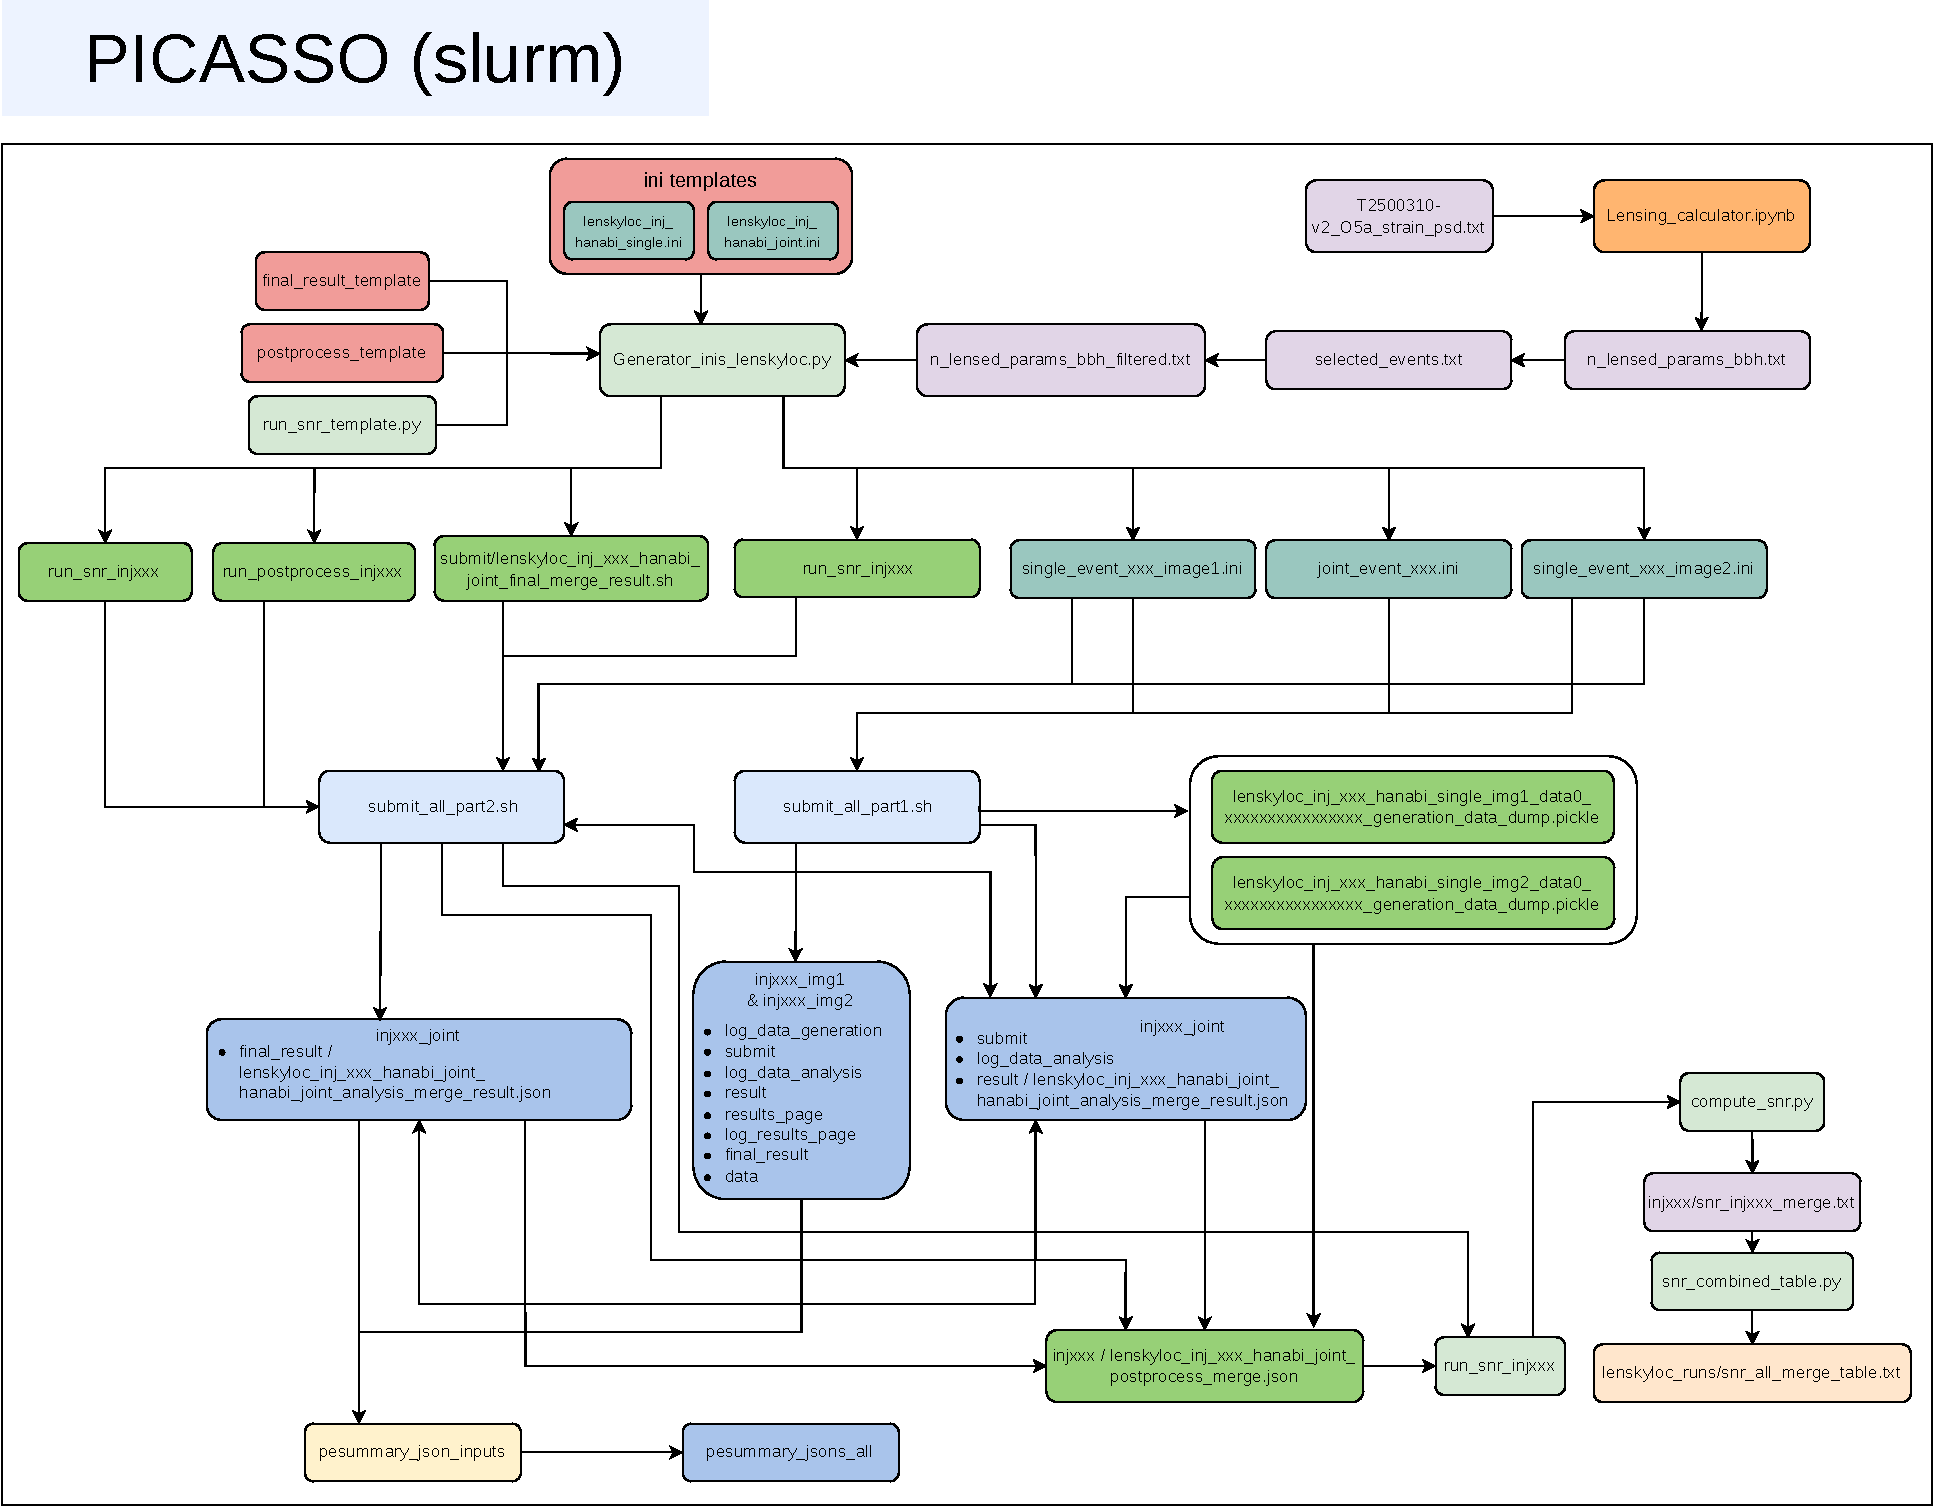
\includegraphics[width=\linewidth]{Figures/diagrama_pipeline_picasso.drawio.pdf}
    \caption[Detailed implementation of the Picasso branch of the pipeline]{Detailed implementation of the Picasso (SLURM) branch of the pipeline, referenced in \S\ref{sec:automation_picasso}. Best viewed digitally, zoomed in. An interactive version with clickable links to each script is available at \url{https://github.com/XxavierGarcia/TFM_reproducibility_material/blob/main/diagrama_pipeline.drawio.pdf} (download to enable links).}
    \label{fig:pipeline_picasso}
\end{figure}

\newpage

\begin{figure}[h!]
    \centering
    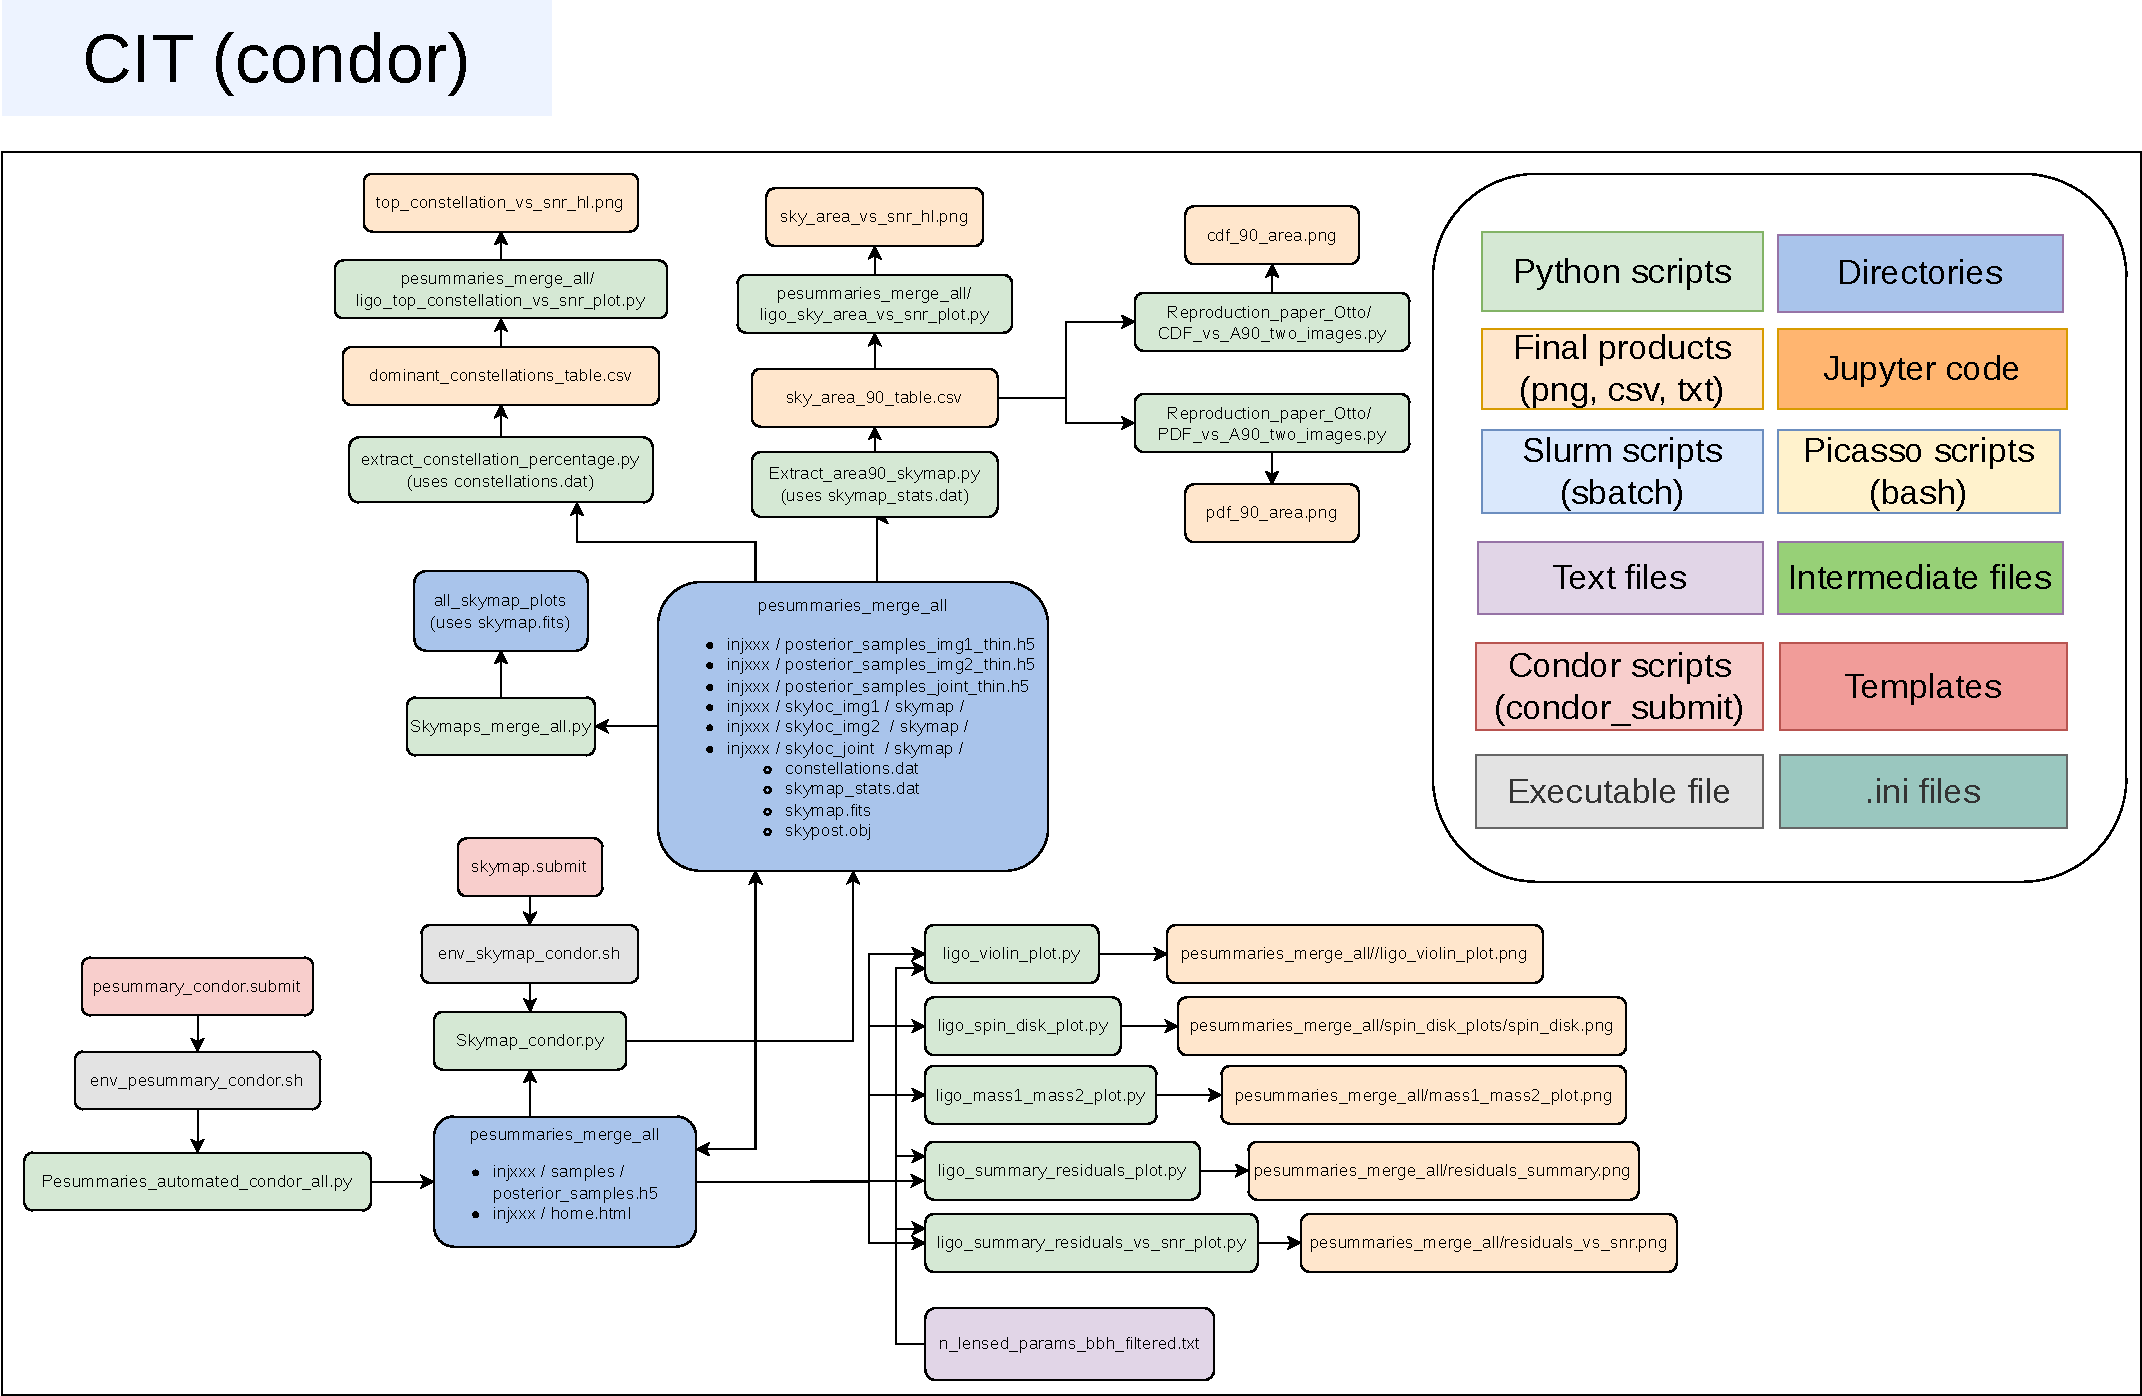
\includegraphics[width=\linewidth]{Figures/diagrama_pipeline_CIT.drawio.pdf}
    \caption[Detailed implementation of the CIT branch of the pipeline]{Detailed implementation of the CIT (HTCondor) post-processing branch of the pipeline, referenced in \S\ref{sec:automation_picasso} and \S\ref{sec:skymap_generation}. Best viewed digitally, zoomed in. An interactive version with clickable links to each script is available at \url{https://github.com/XxavierGarcia/TFM_reproducibility_material/blob/main/diagrama_pipeline.drawio.pdf} (download to enable links).}
    \label{fig:pipeline_cit}
\end{figure}




\renewcommand{\thechapter}{D}
\chapter{Full posterior comparison for all events}
\label{app:violins}

This appendix collects the recovered posteriors for all 150 analyzed events, complementing the representative examples and population-level residuals of \S\ref{sec:parameter_recovery}. For each event, the joint posterior (green, solid) is shown together with the two single-image posteriors (red dash-dot for image 1, blue dotted for image 2) and the injected value (black tick). Figure~\ref{fig:violin_massdist_full} shows the chirp mass, mass ratio, and effective luminosity distance; Figure~\ref{fig:violin_spins_full} shows the spin parameters. Within each set the events are ordered by injection index and split across pages.


% Set A: chirp mass, mass ratio, effective distance

\begin{figure}[p]
    \centering
    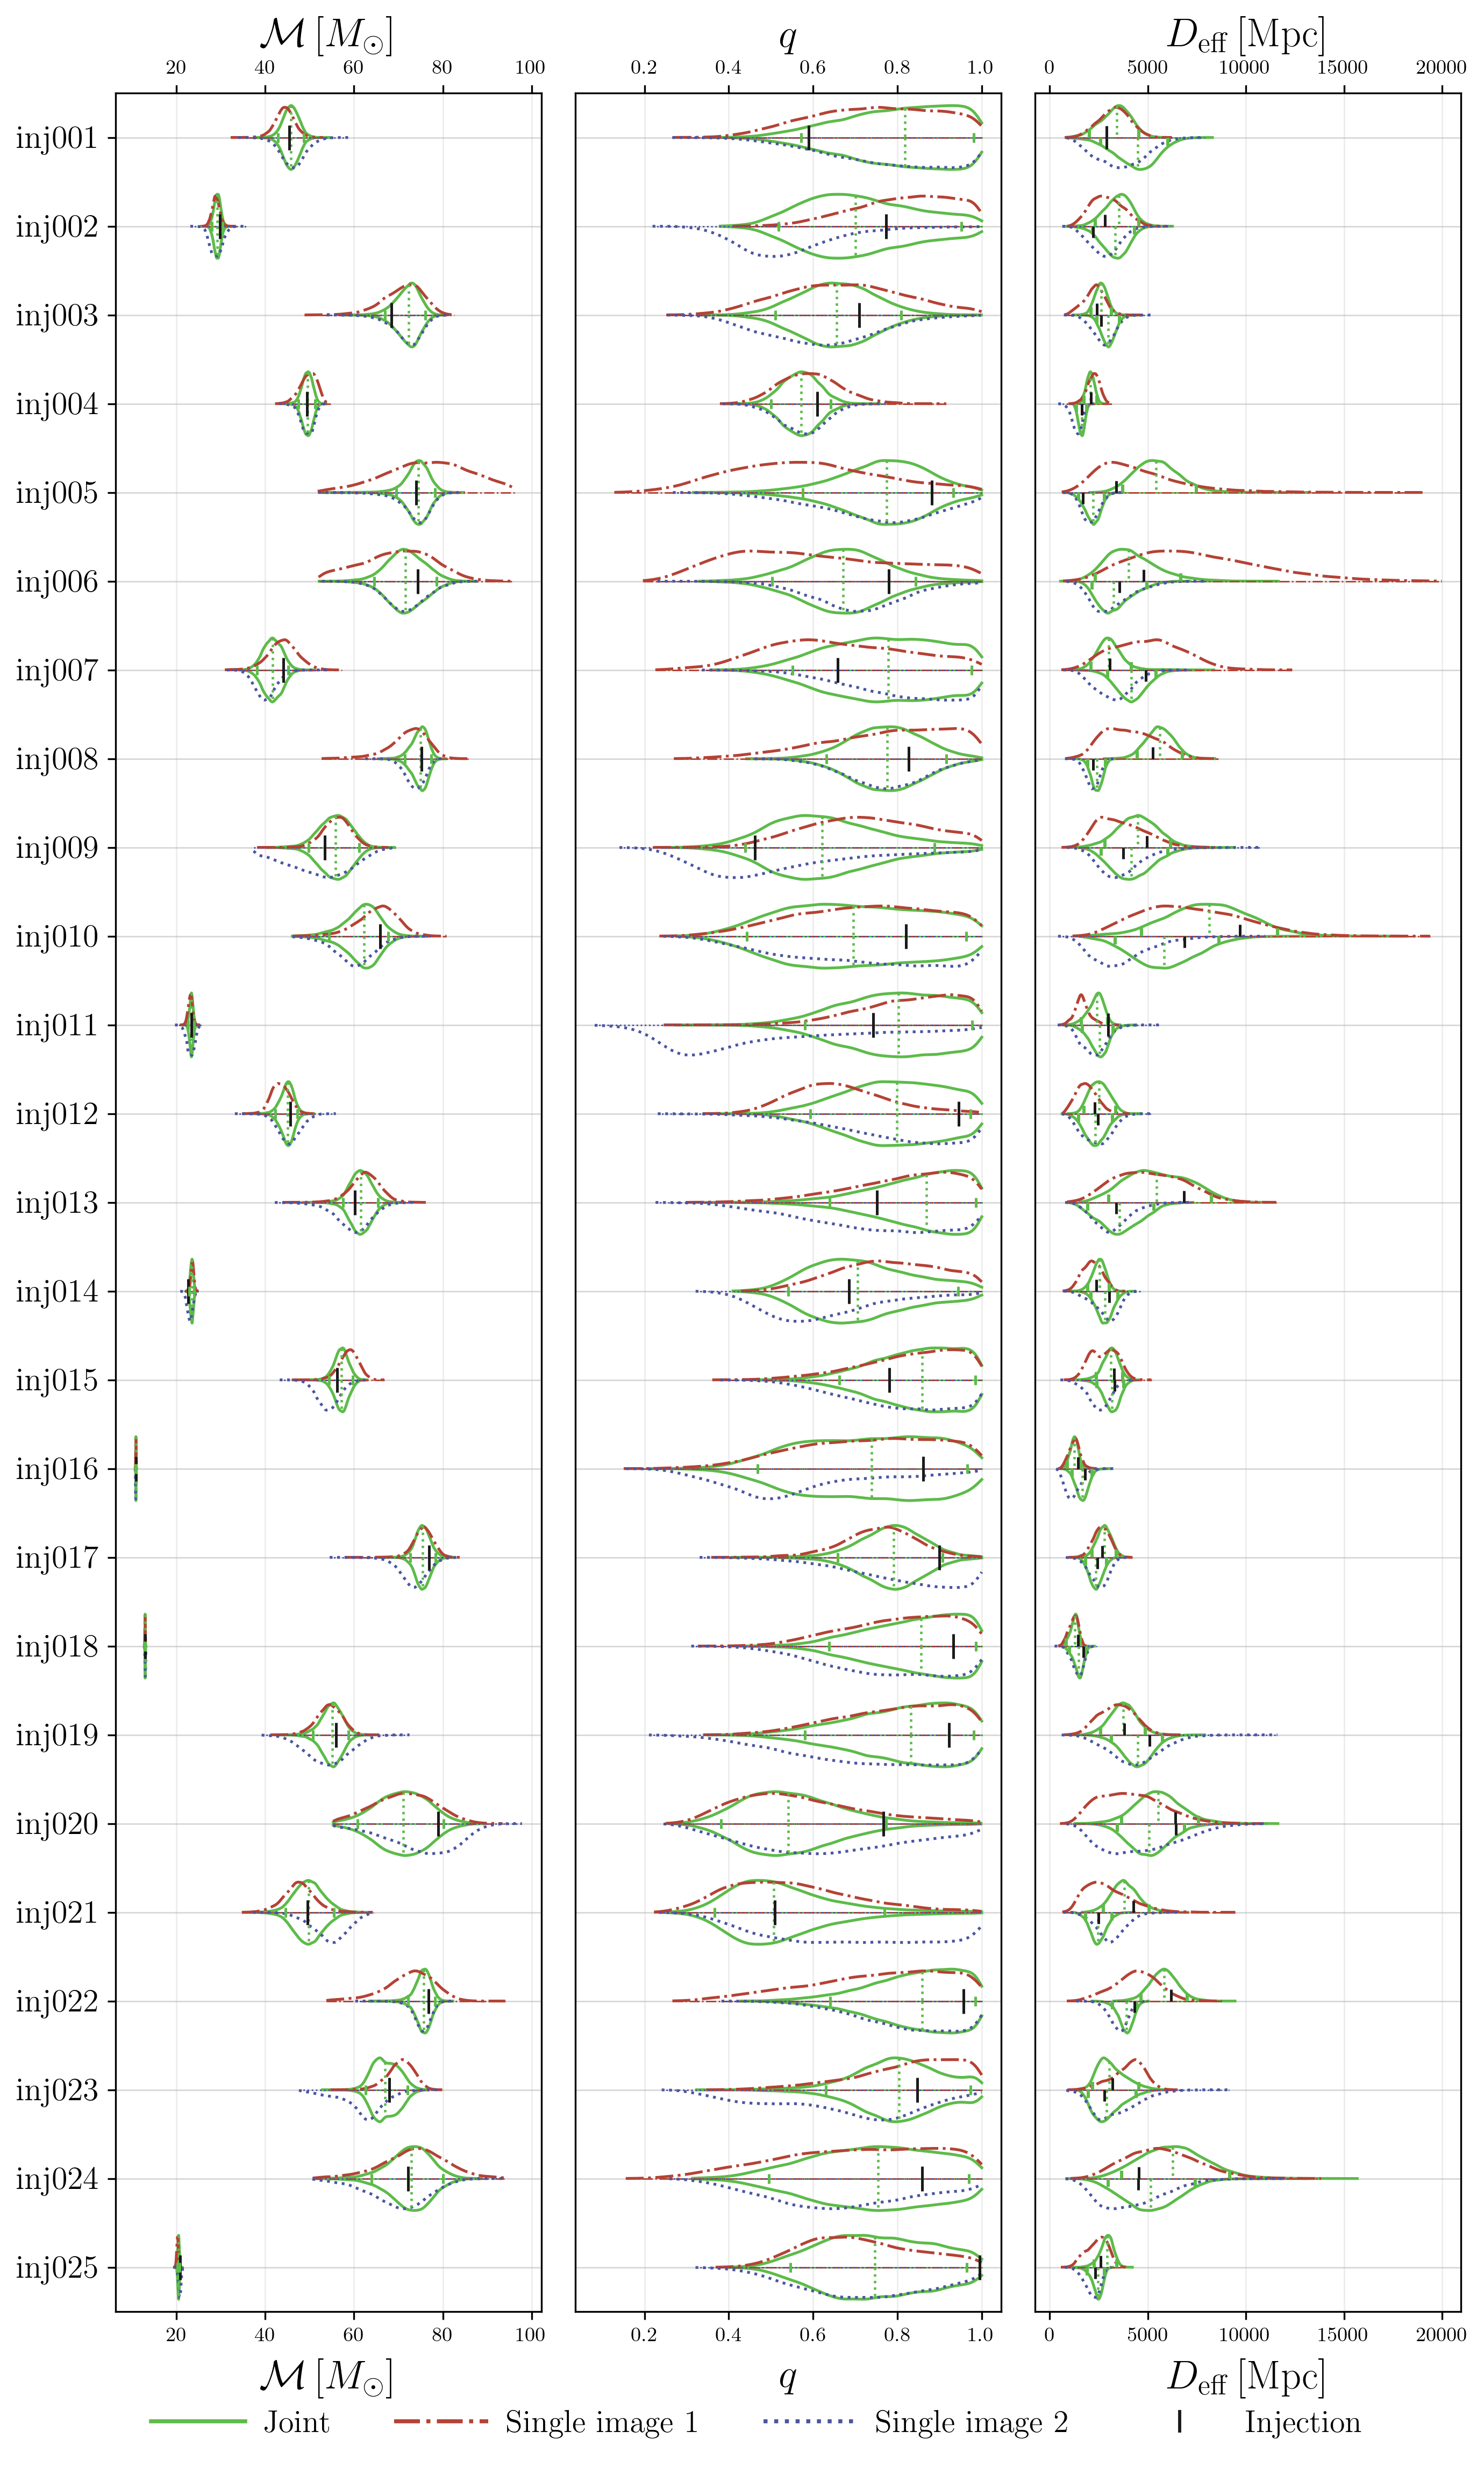
\includegraphics[height=0.92\textheight]{Figures/violin_massdist_p01.png}
    \caption[Posteriors for all events: chirp mass, mass ratio, effective distance]{Recovered posteriors of the chirp mass $\mathcal{M}$, mass ratio $q$, and effective luminosity distance $D_\mathrm{eff}$, for all 150 events (1 of 5). Joint posterior in green (solid), single-image posteriors in red (dash-dot, image 1) and blue (dotted, image 2); the injected value is the black tick.}
    \label{fig:violin_massdist_full}
\end{figure}

\begin{figure}[p]
    \ContinuedFloat
    \centering
    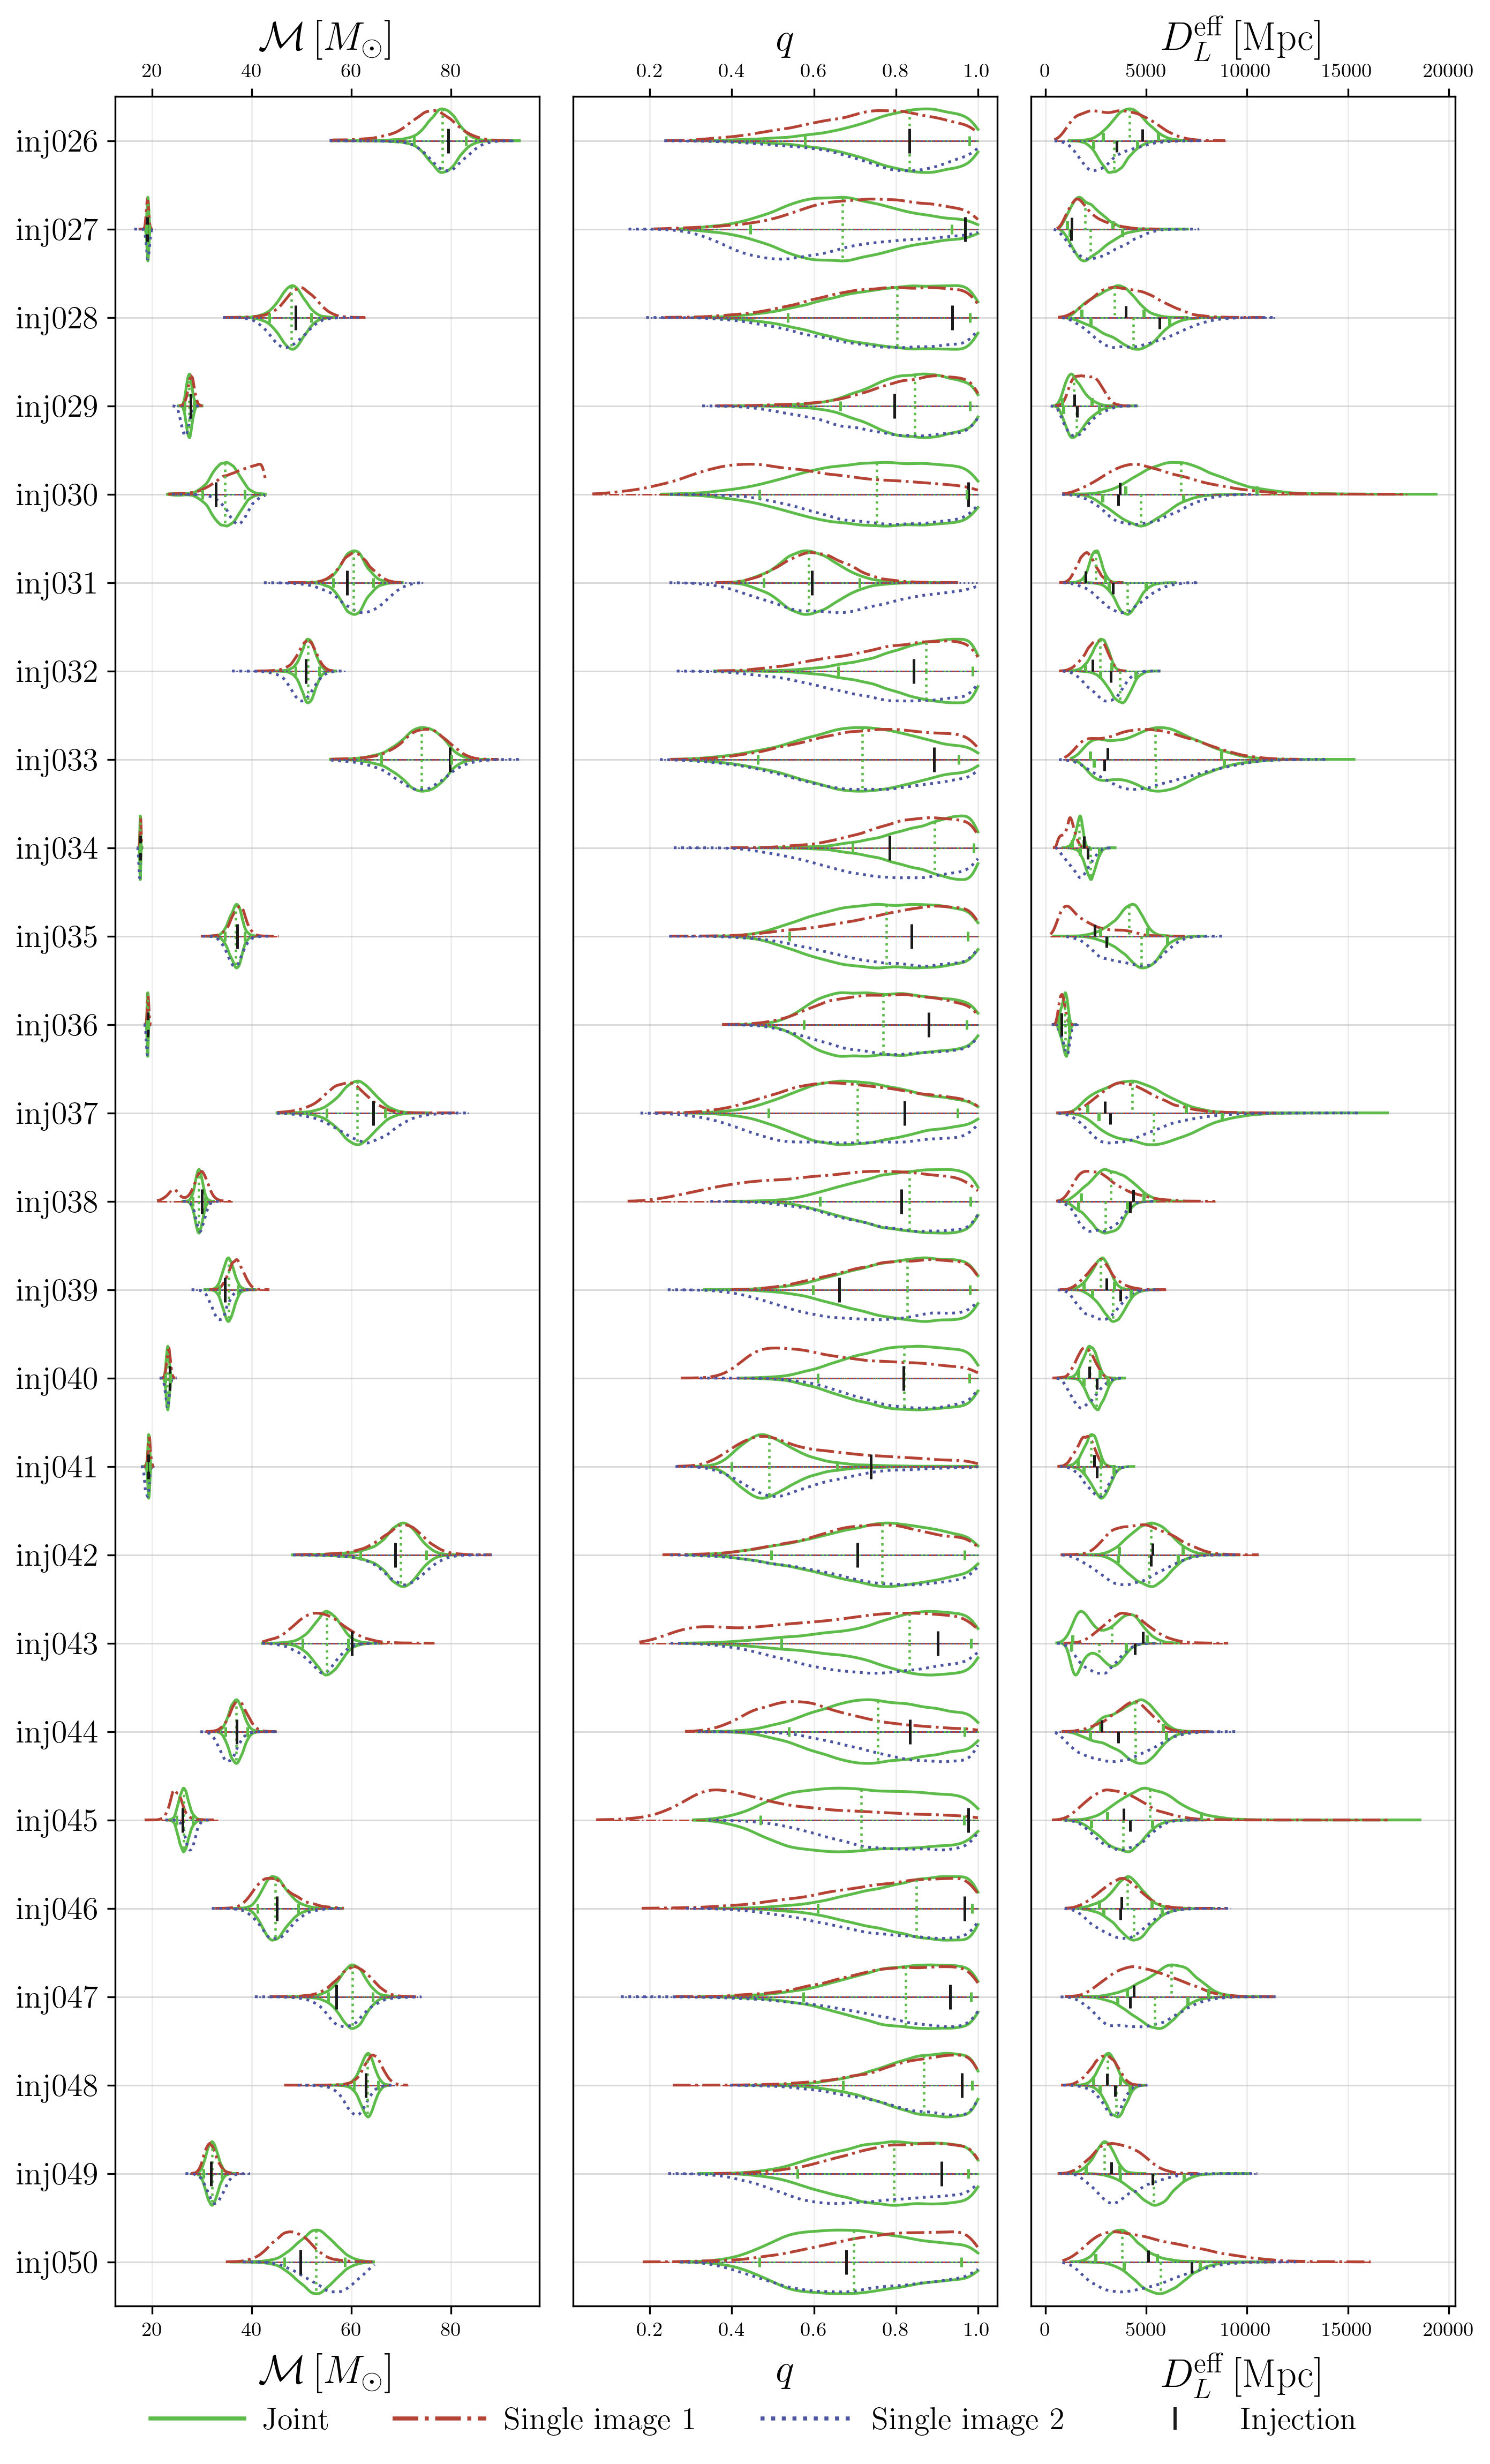
\includegraphics[height=0.92\textheight]{Figures/violin_massdist_p02.png}
    \caption[]{Recovered posteriors of $\mathcal{M}$, $q$, and $D_\mathrm{eff}$ (2 of 5).}
\end{figure}

\begin{figure}[p]
    \ContinuedFloat
    \centering
    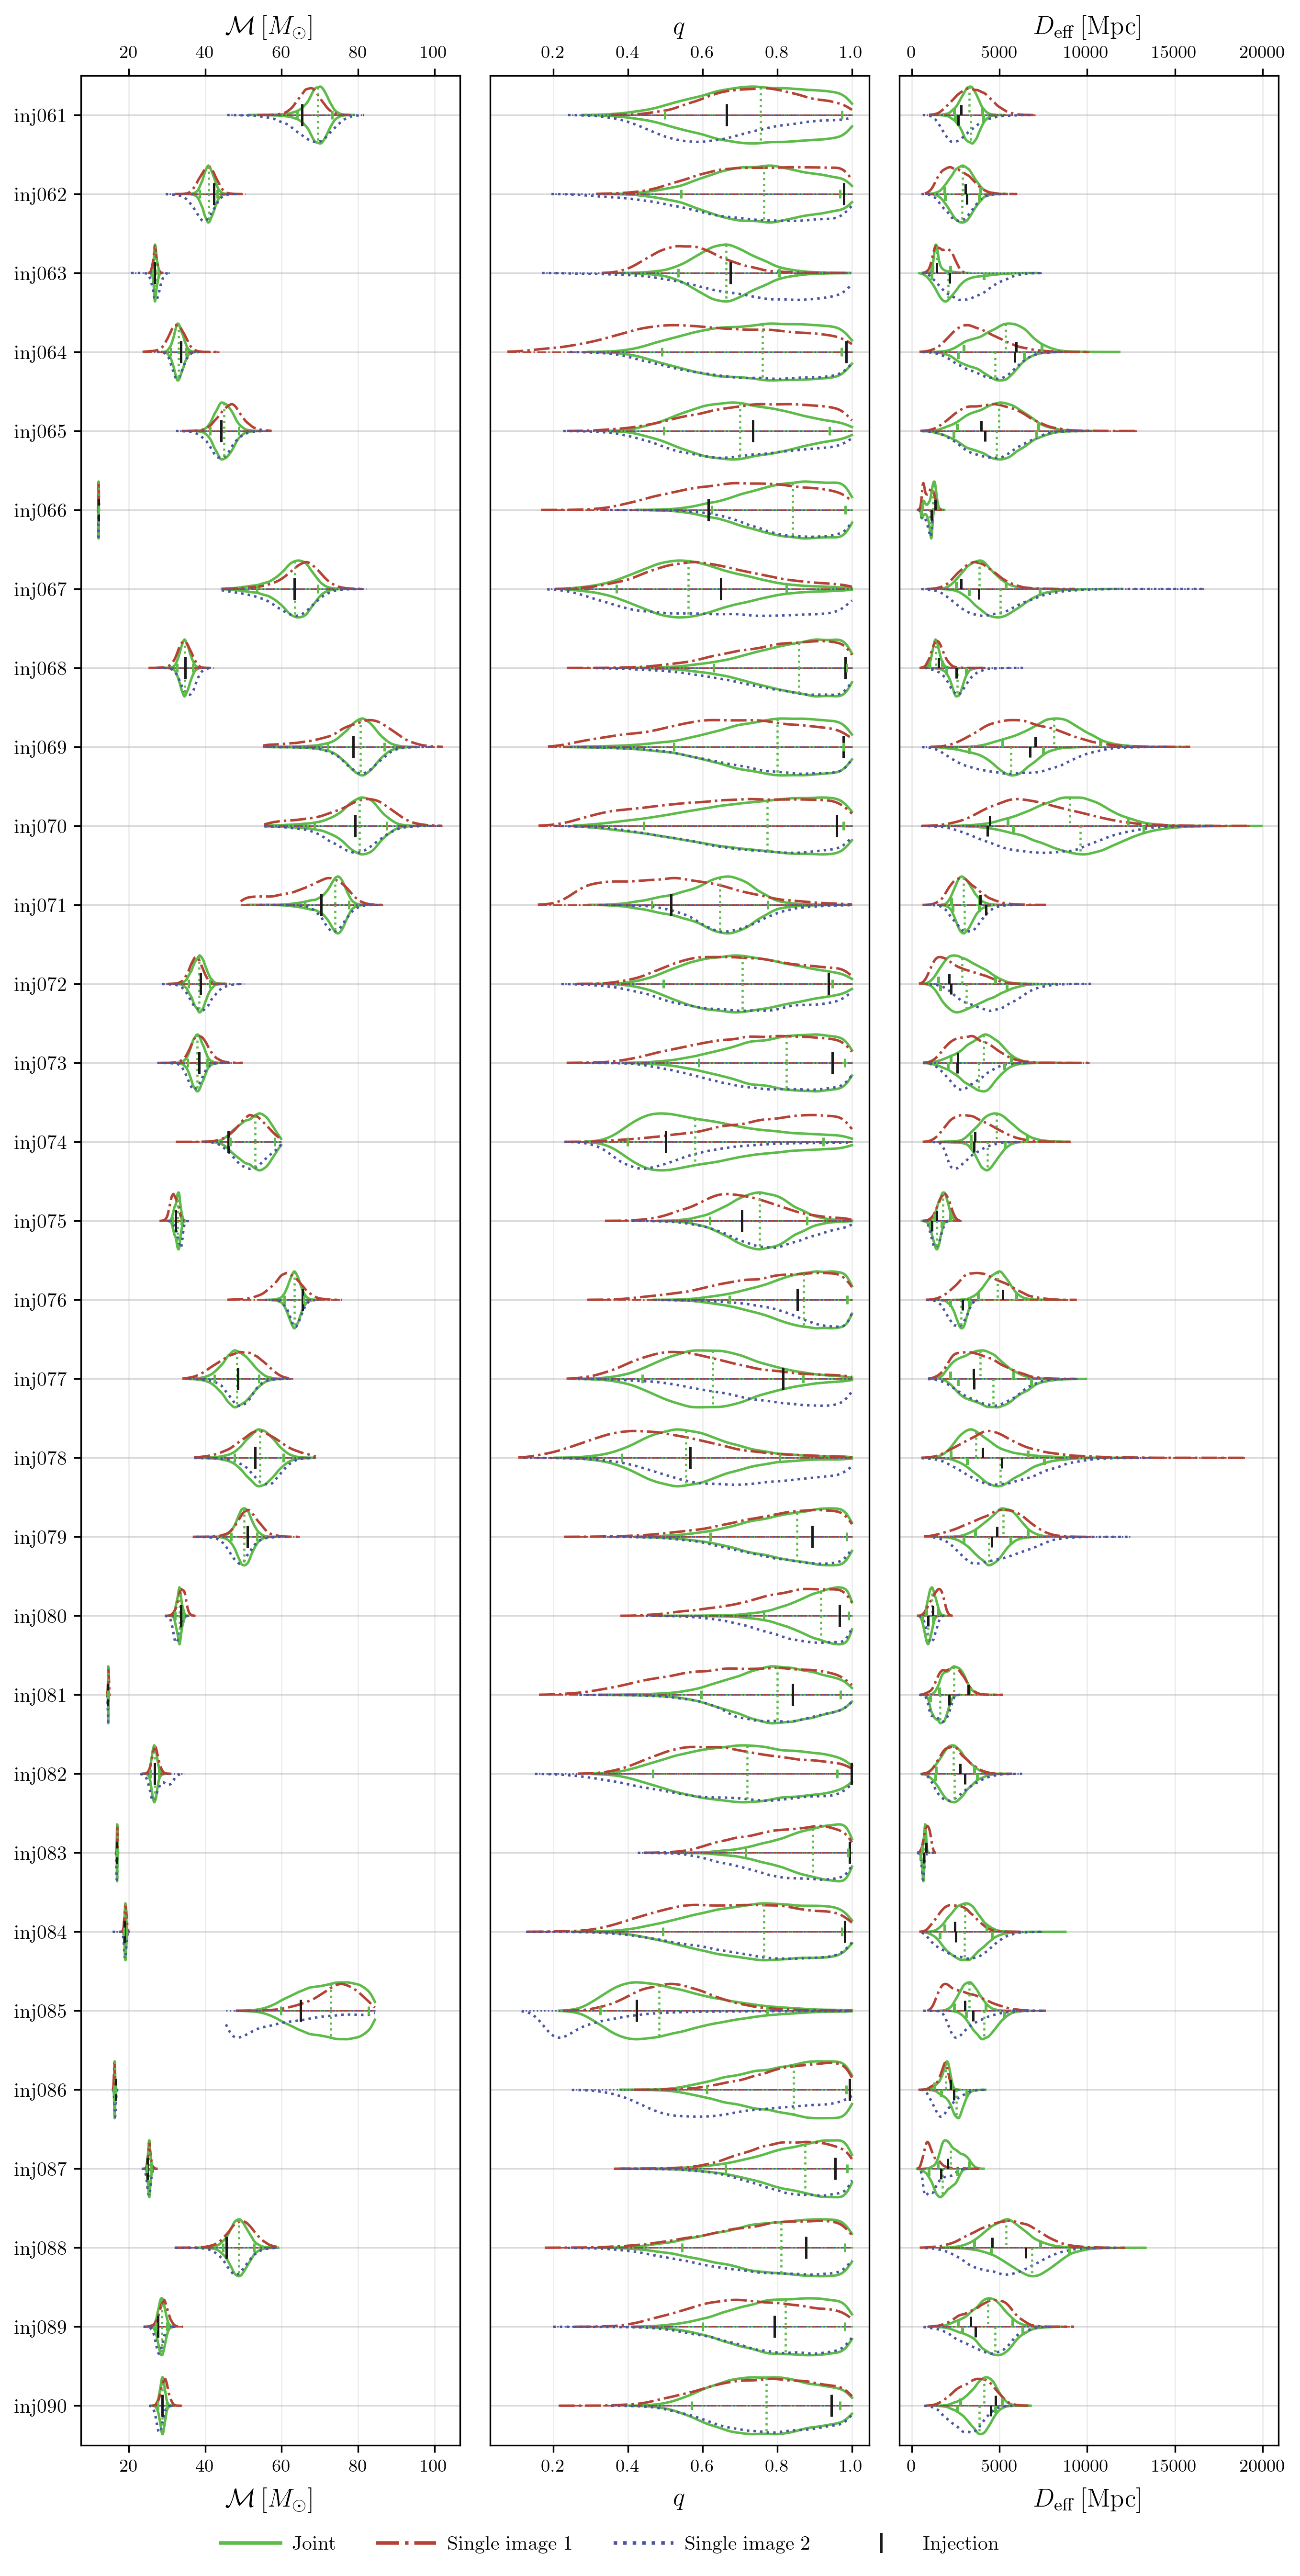
\includegraphics[height=0.92\textheight]{Figures/violin_massdist_p03.png}
    \caption[]{Recovered posteriors of $\mathcal{M}$, $q$, and $D_\mathrm{eff}$ (3 of 5).}
\end{figure}

\begin{figure}[p]
    \ContinuedFloat
    \centering
    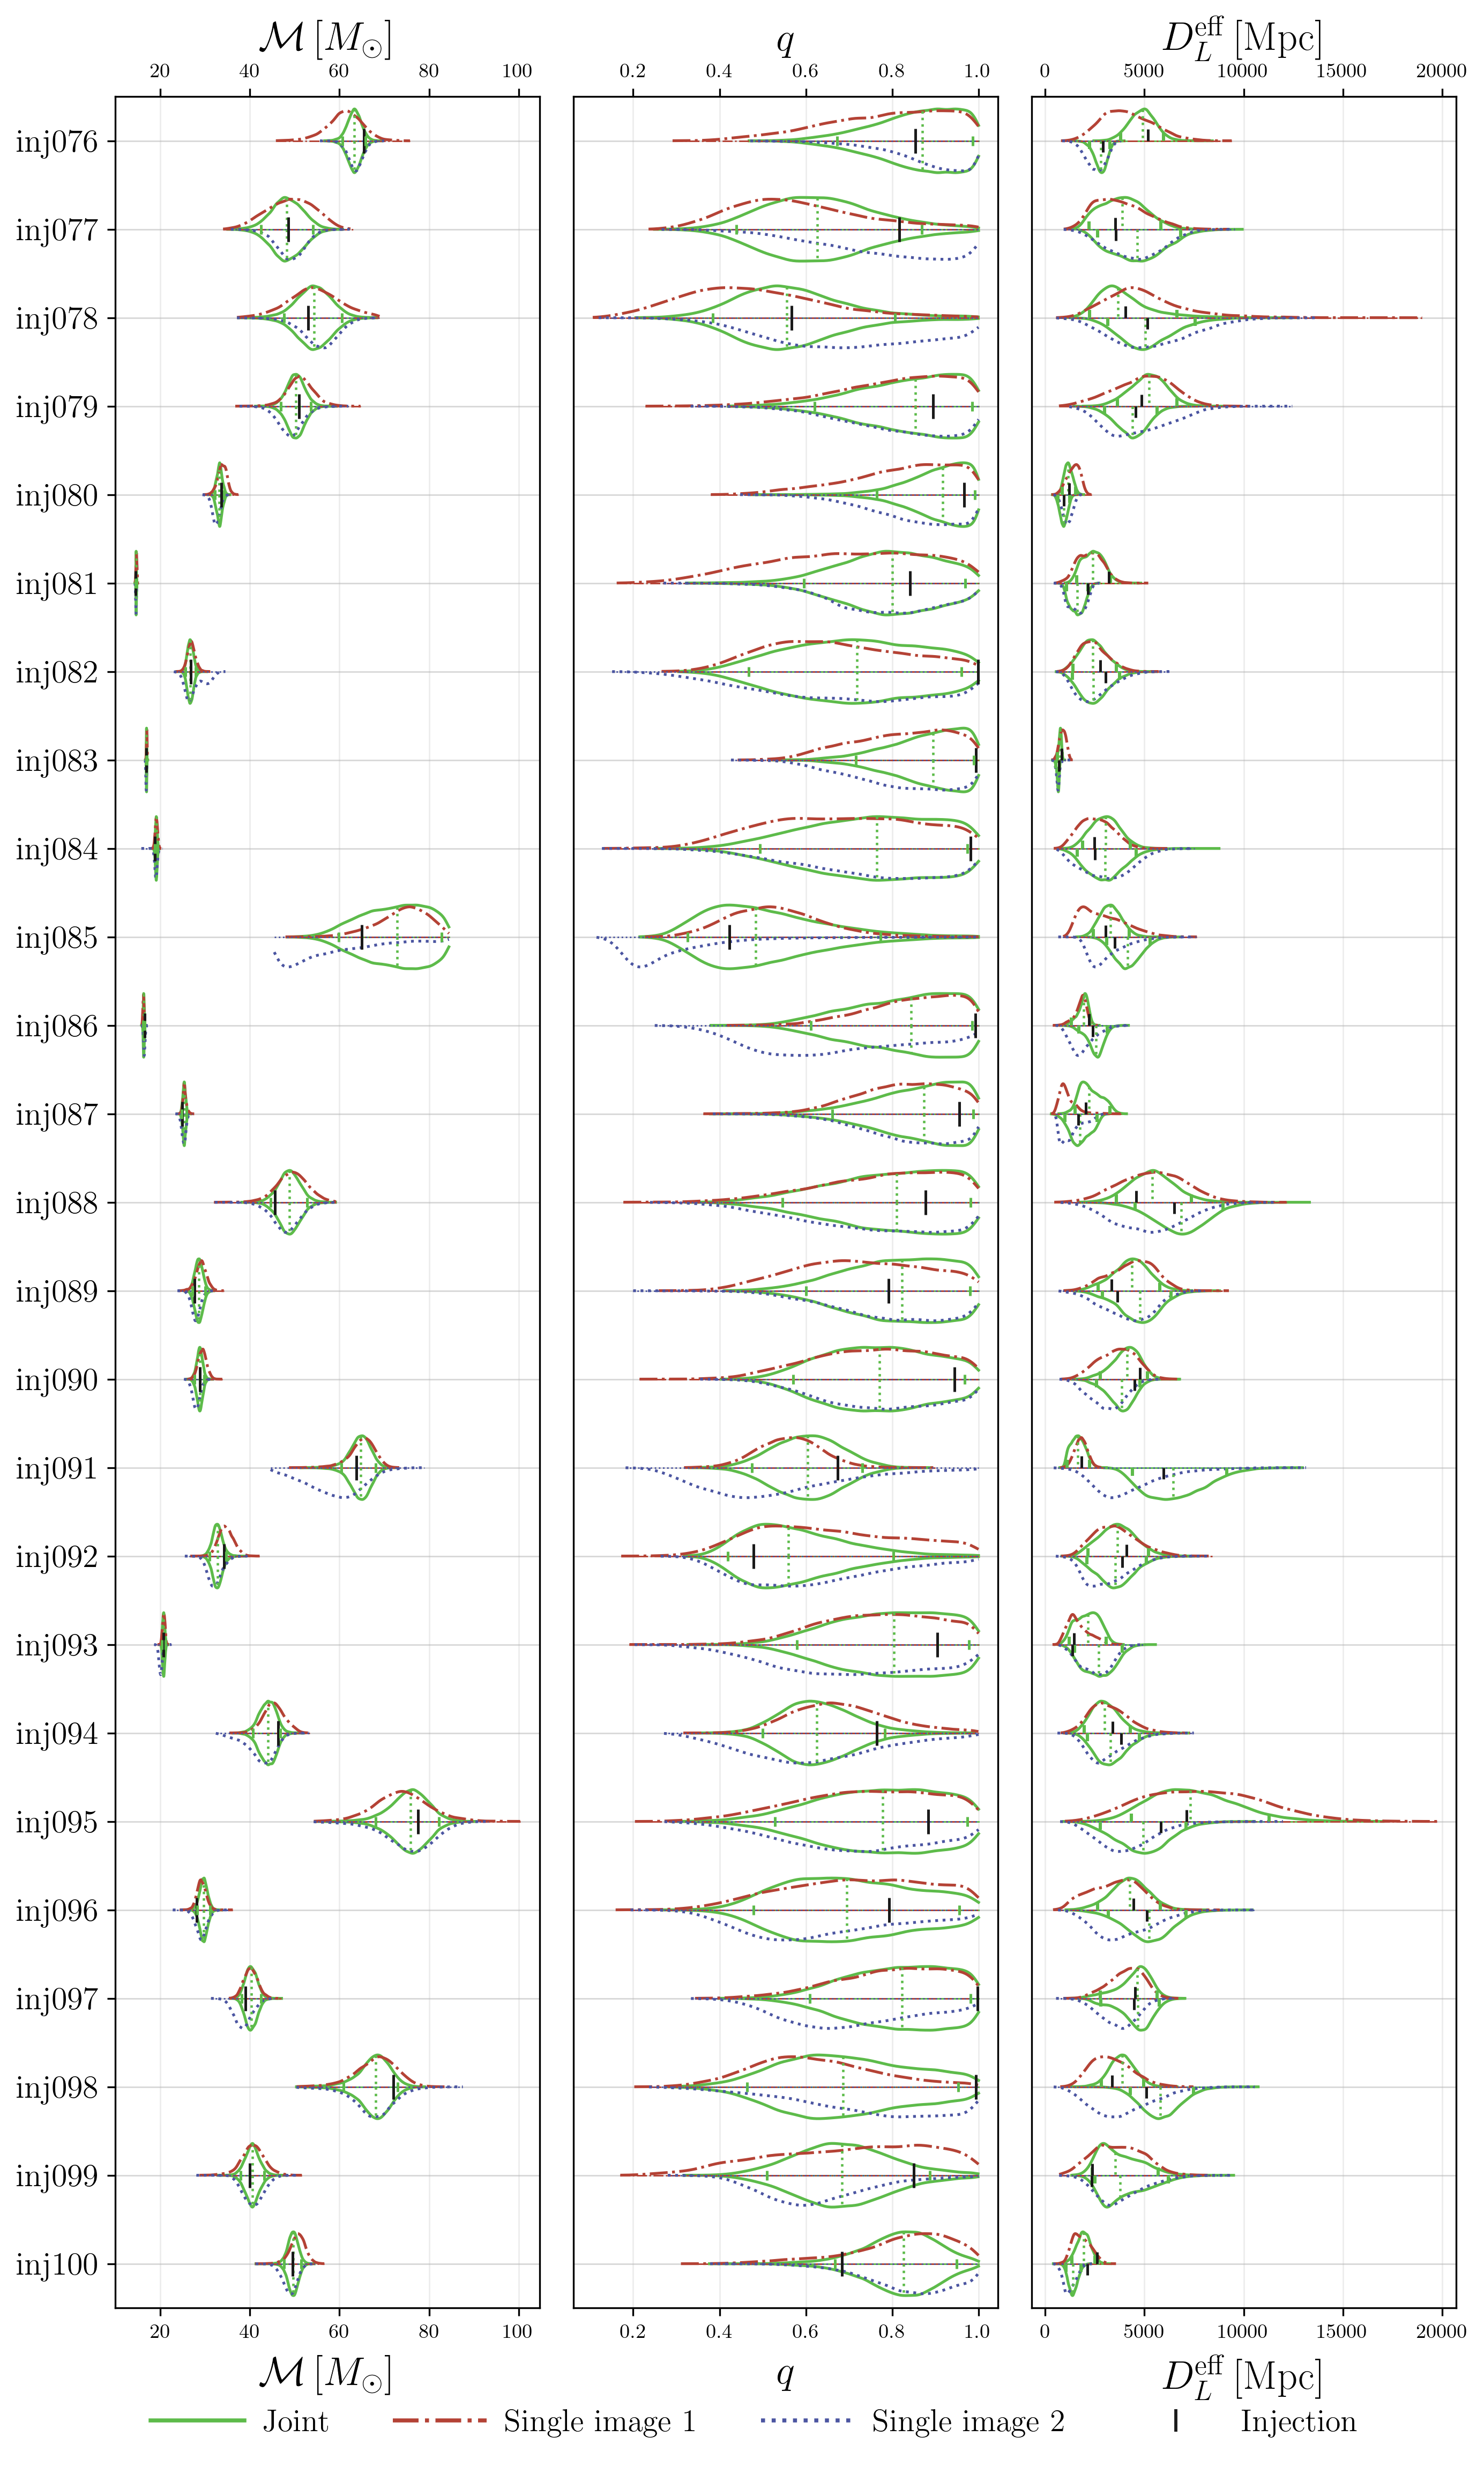
\includegraphics[height=0.92\textheight]{Figures/violin_massdist_p04.png}
    \caption[]{Recovered posteriors of $\mathcal{M}$, $q$, and $D_\mathrm{eff}$ (4 of 5).}
\end{figure}

\begin{figure}[p]
    \ContinuedFloat
    \centering
    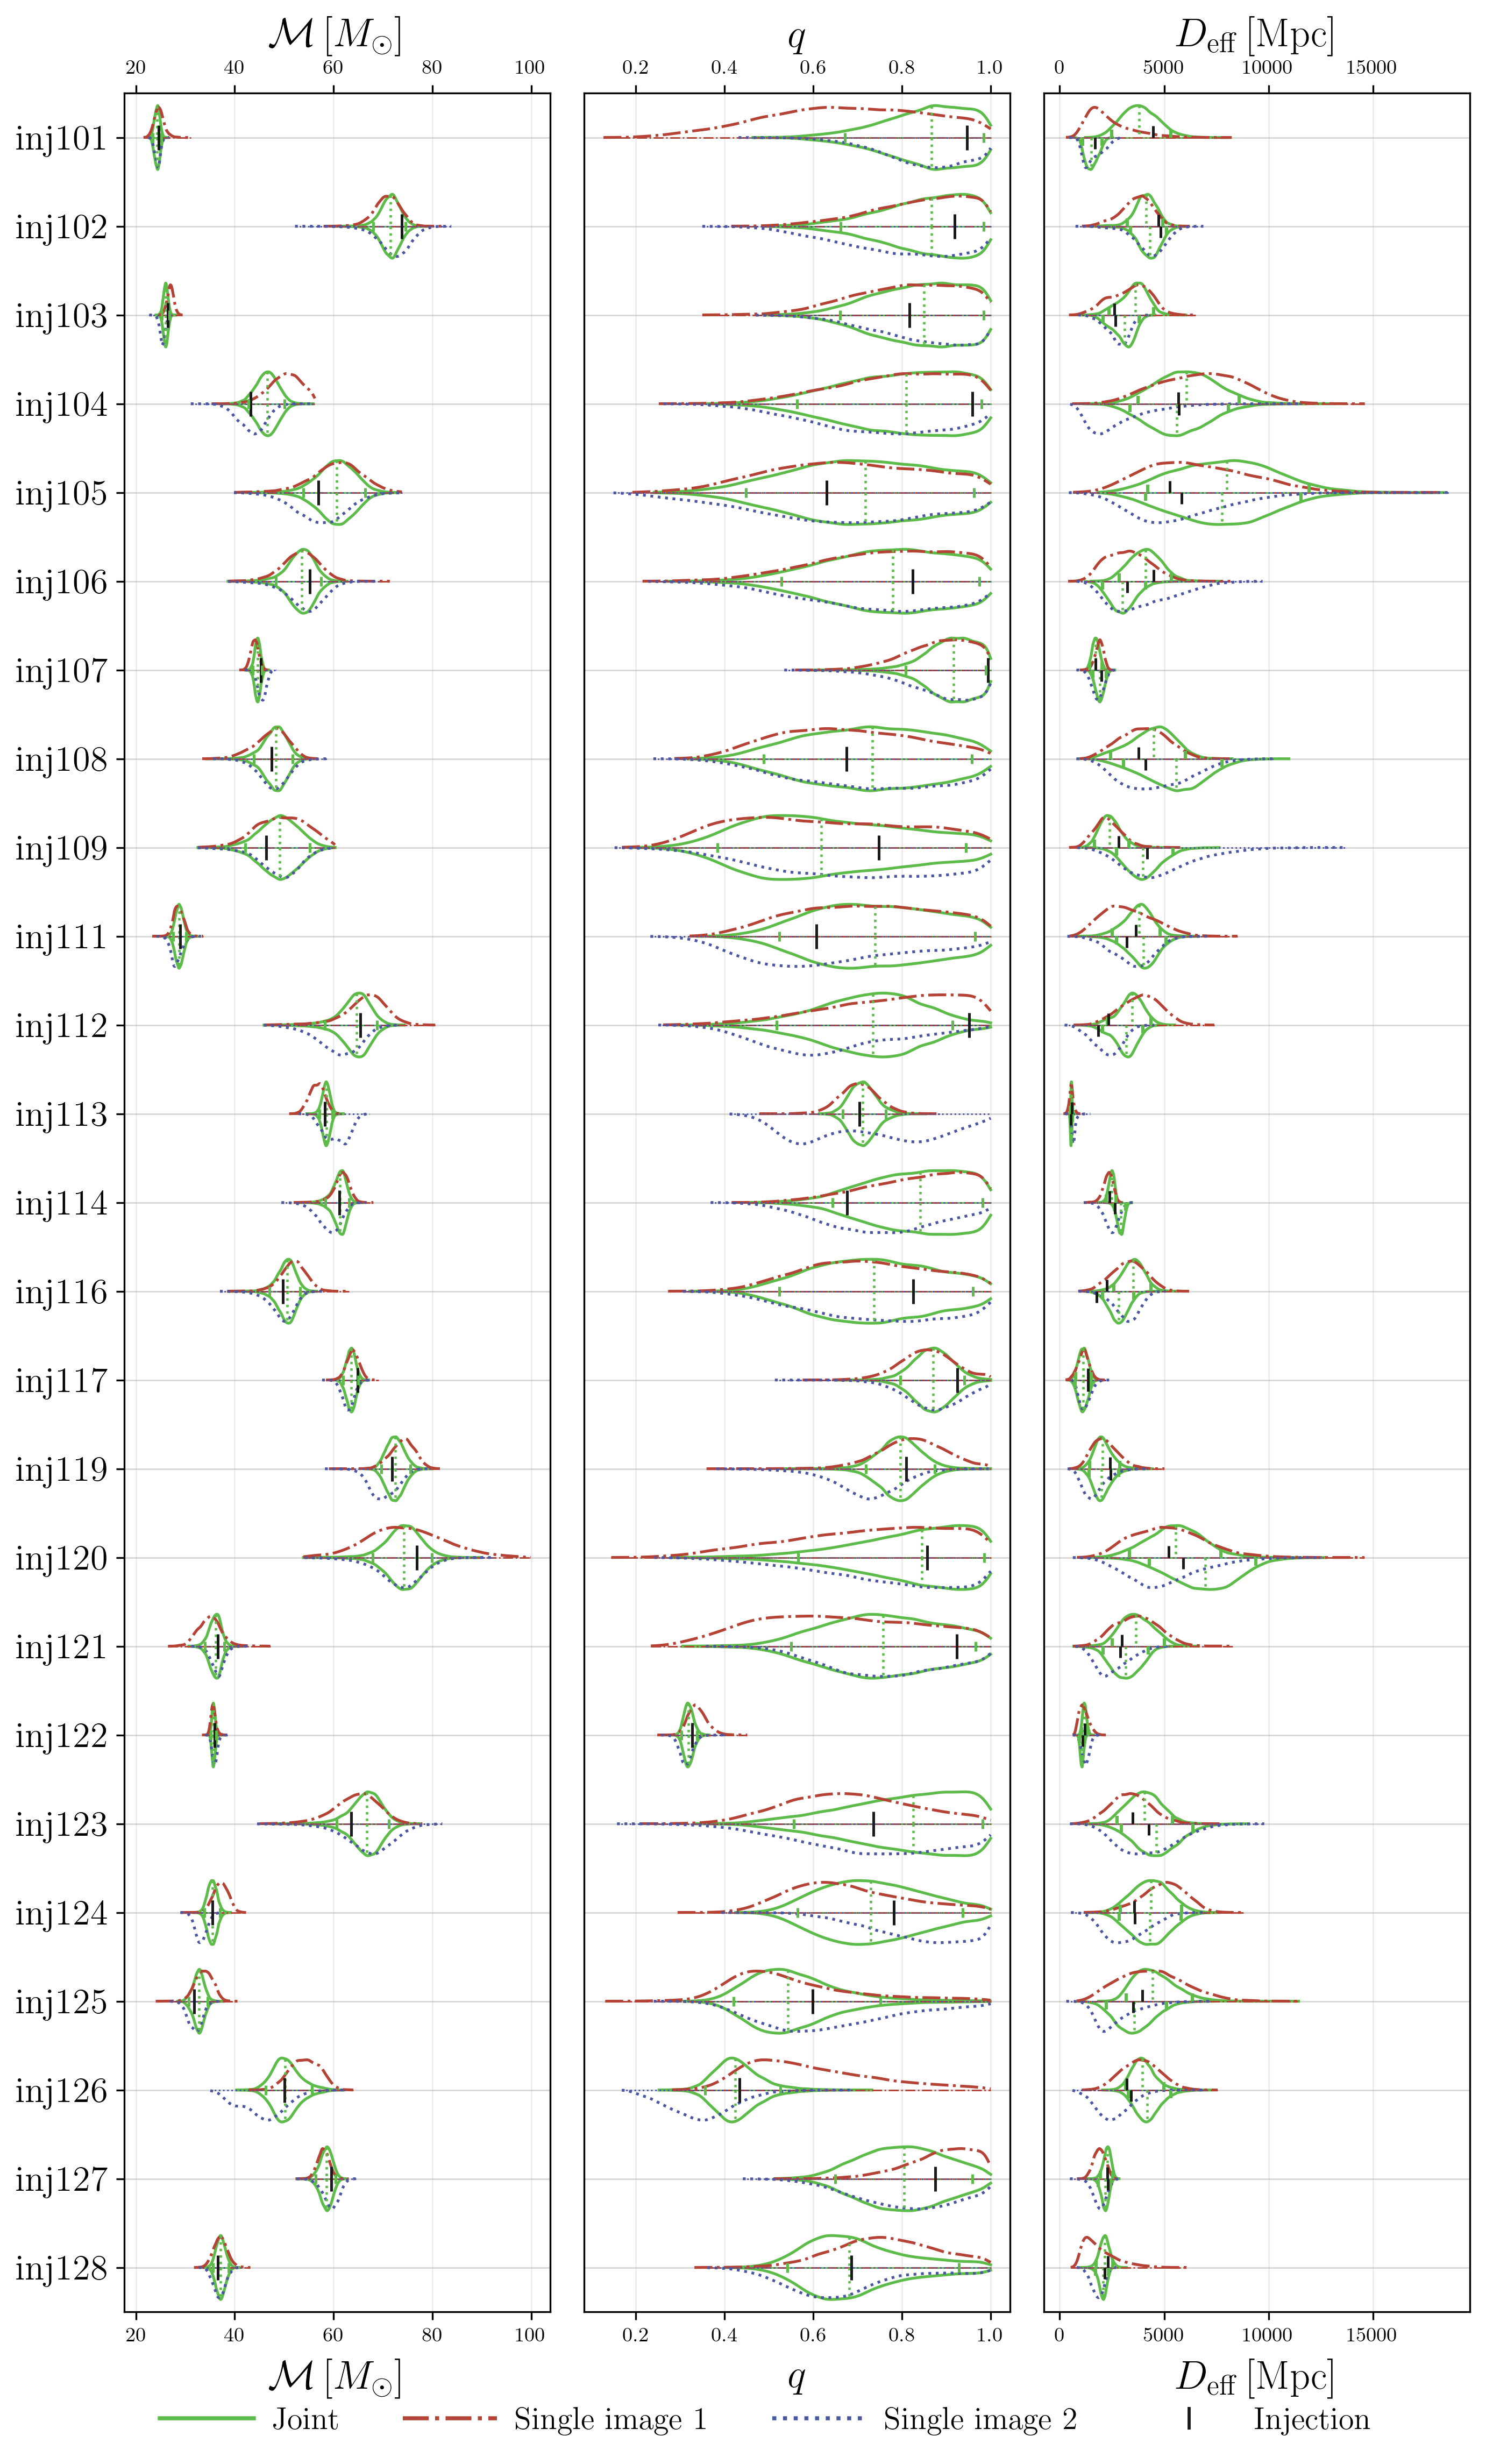
\includegraphics[height=0.92\textheight]{Figures/violin_massdist_p05.png}
    \caption[]{Recovered posteriors of $\mathcal{M}$, $q$, and $D_\mathrm{eff}$ (5 of 5).}
\end{figure}


% Set B: spin parameters

\begin{figure}[p]
    \centering
    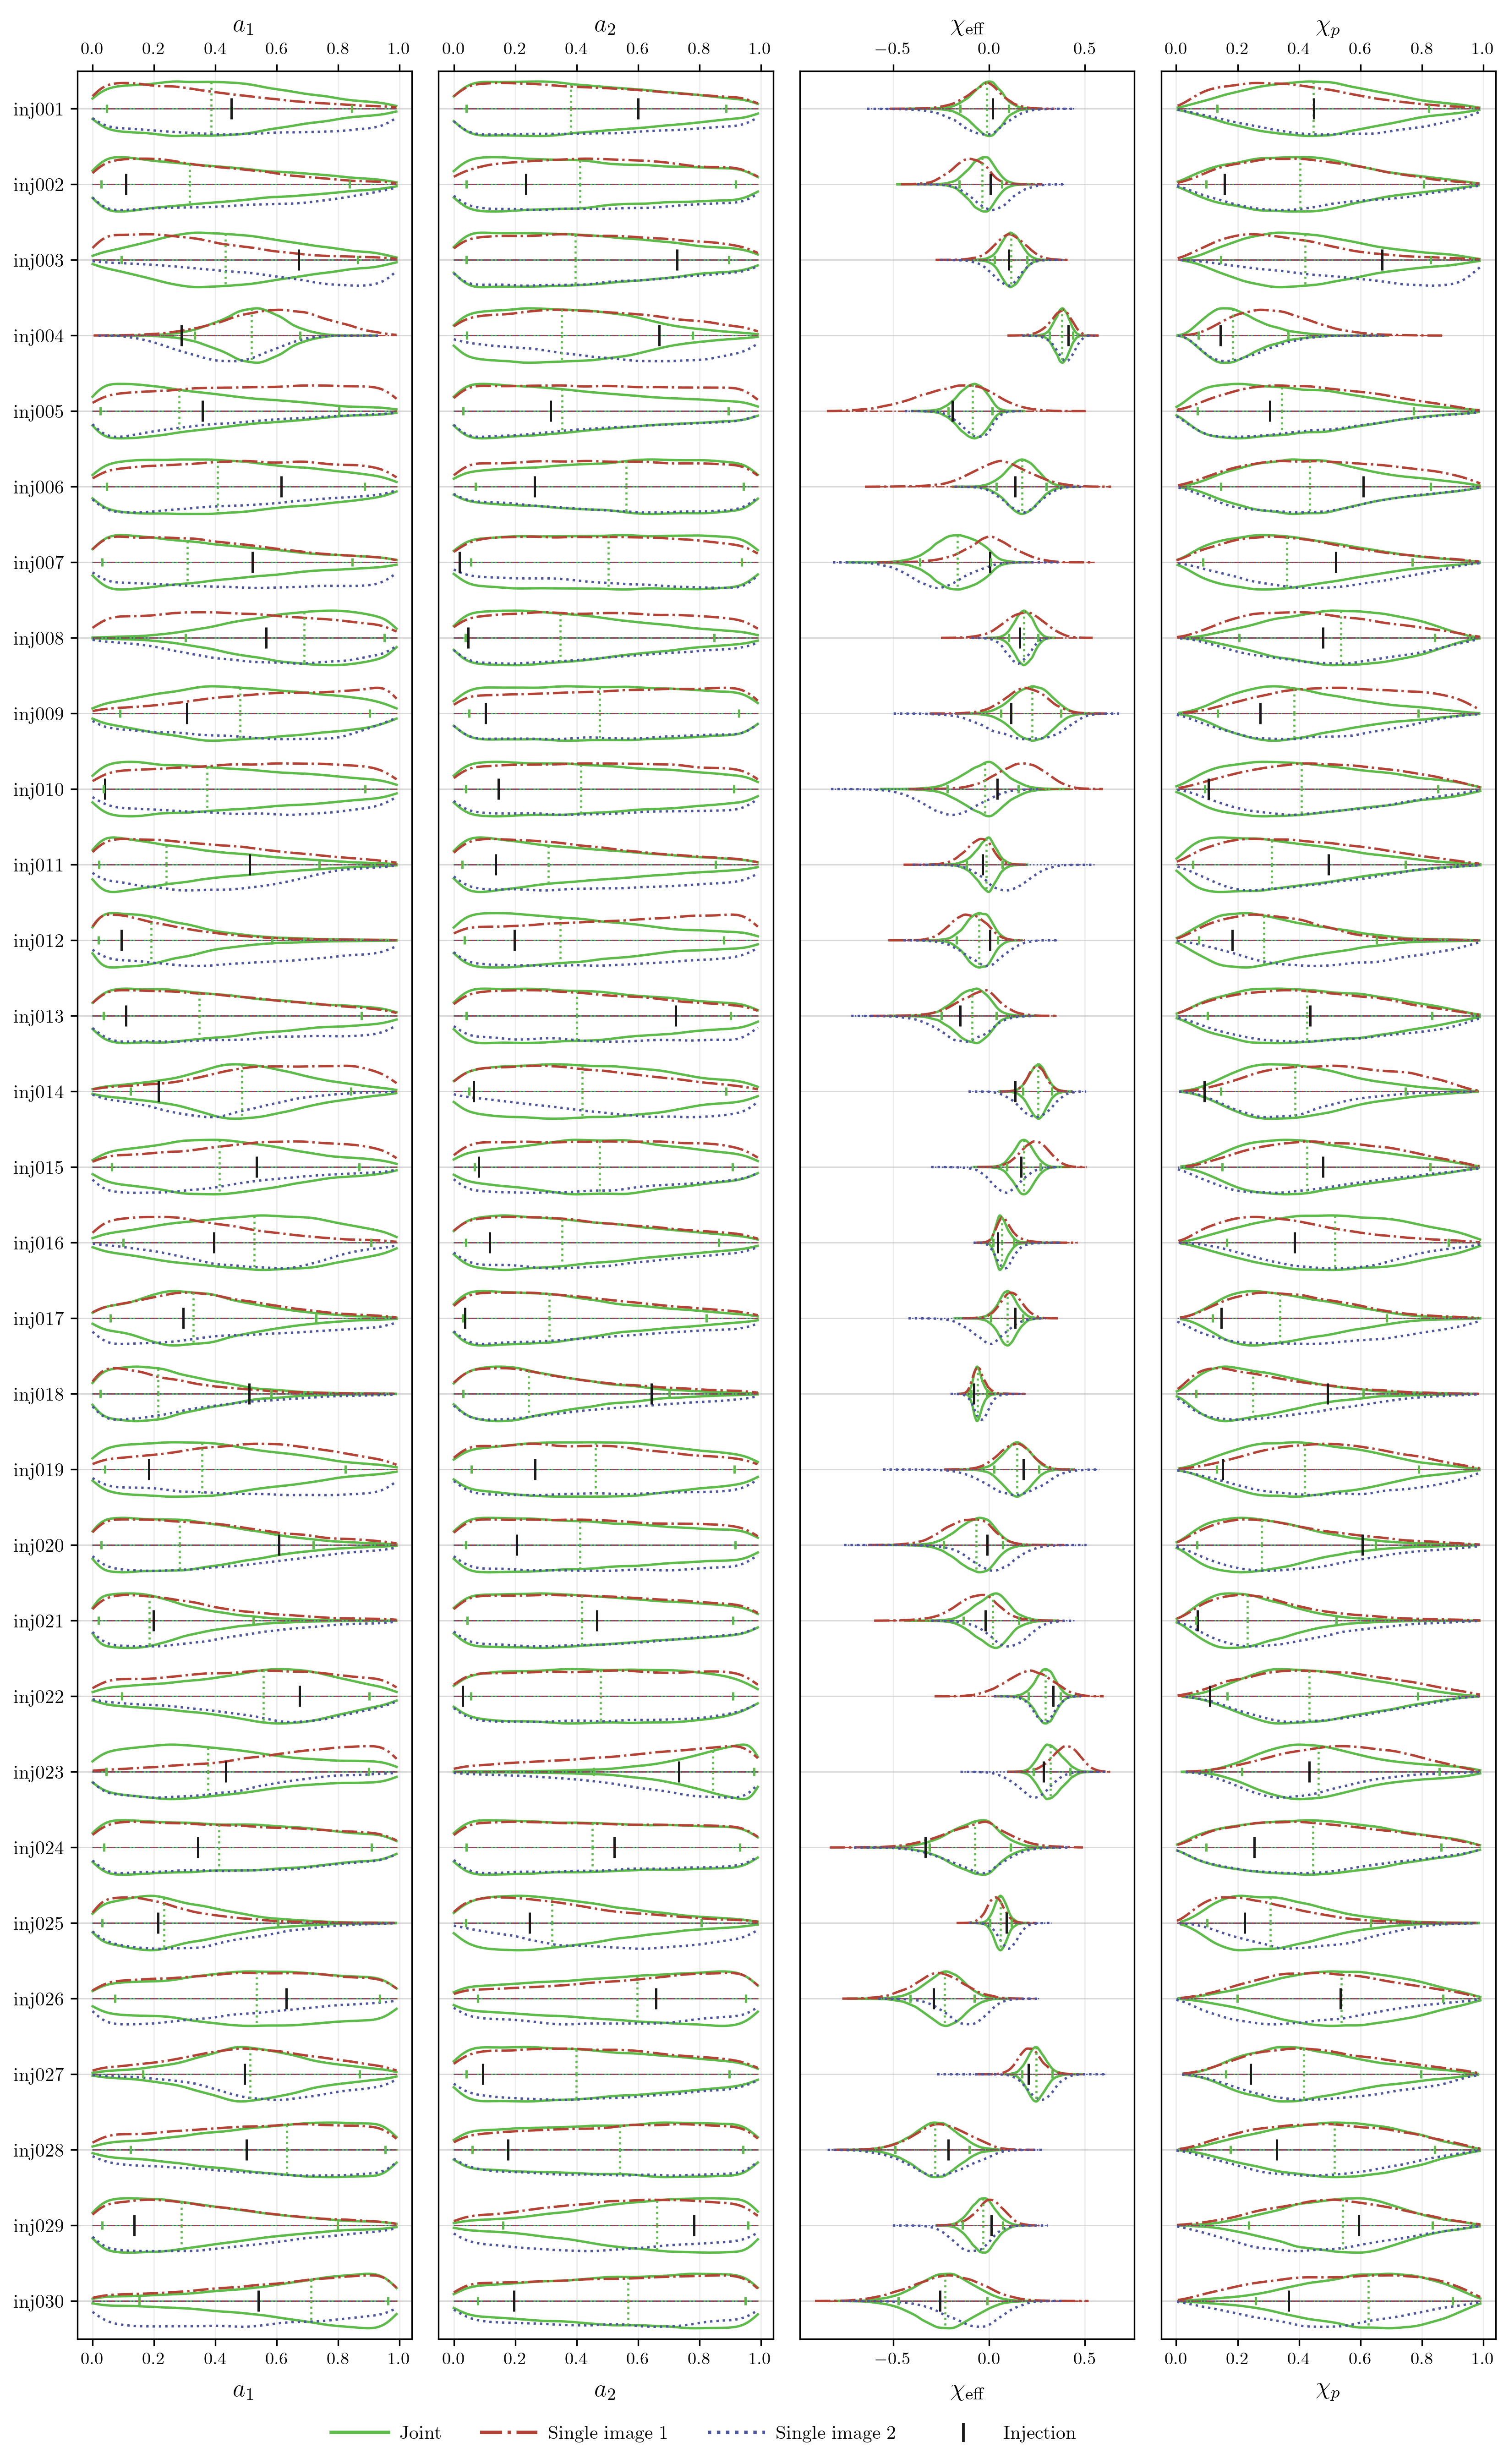
\includegraphics[height=0.92\textheight]{Figures/violin_spins_p01.png}
    \caption[Posteriors for all events: spin parameters]{Recovered posteriors of the spin magnitudes $a_1$ and $a_2$, effective spin $\chi_\mathrm{eff}$, and precessing spin $\chi_\mathrm{p}$, for all 150 events (1 of 5). Colors as in Figure~\ref{fig:violin_massdist_full}.}
    \label{fig:violin_spins_full}
\end{figure}

\begin{figure}[p]
    \ContinuedFloat
    \centering
    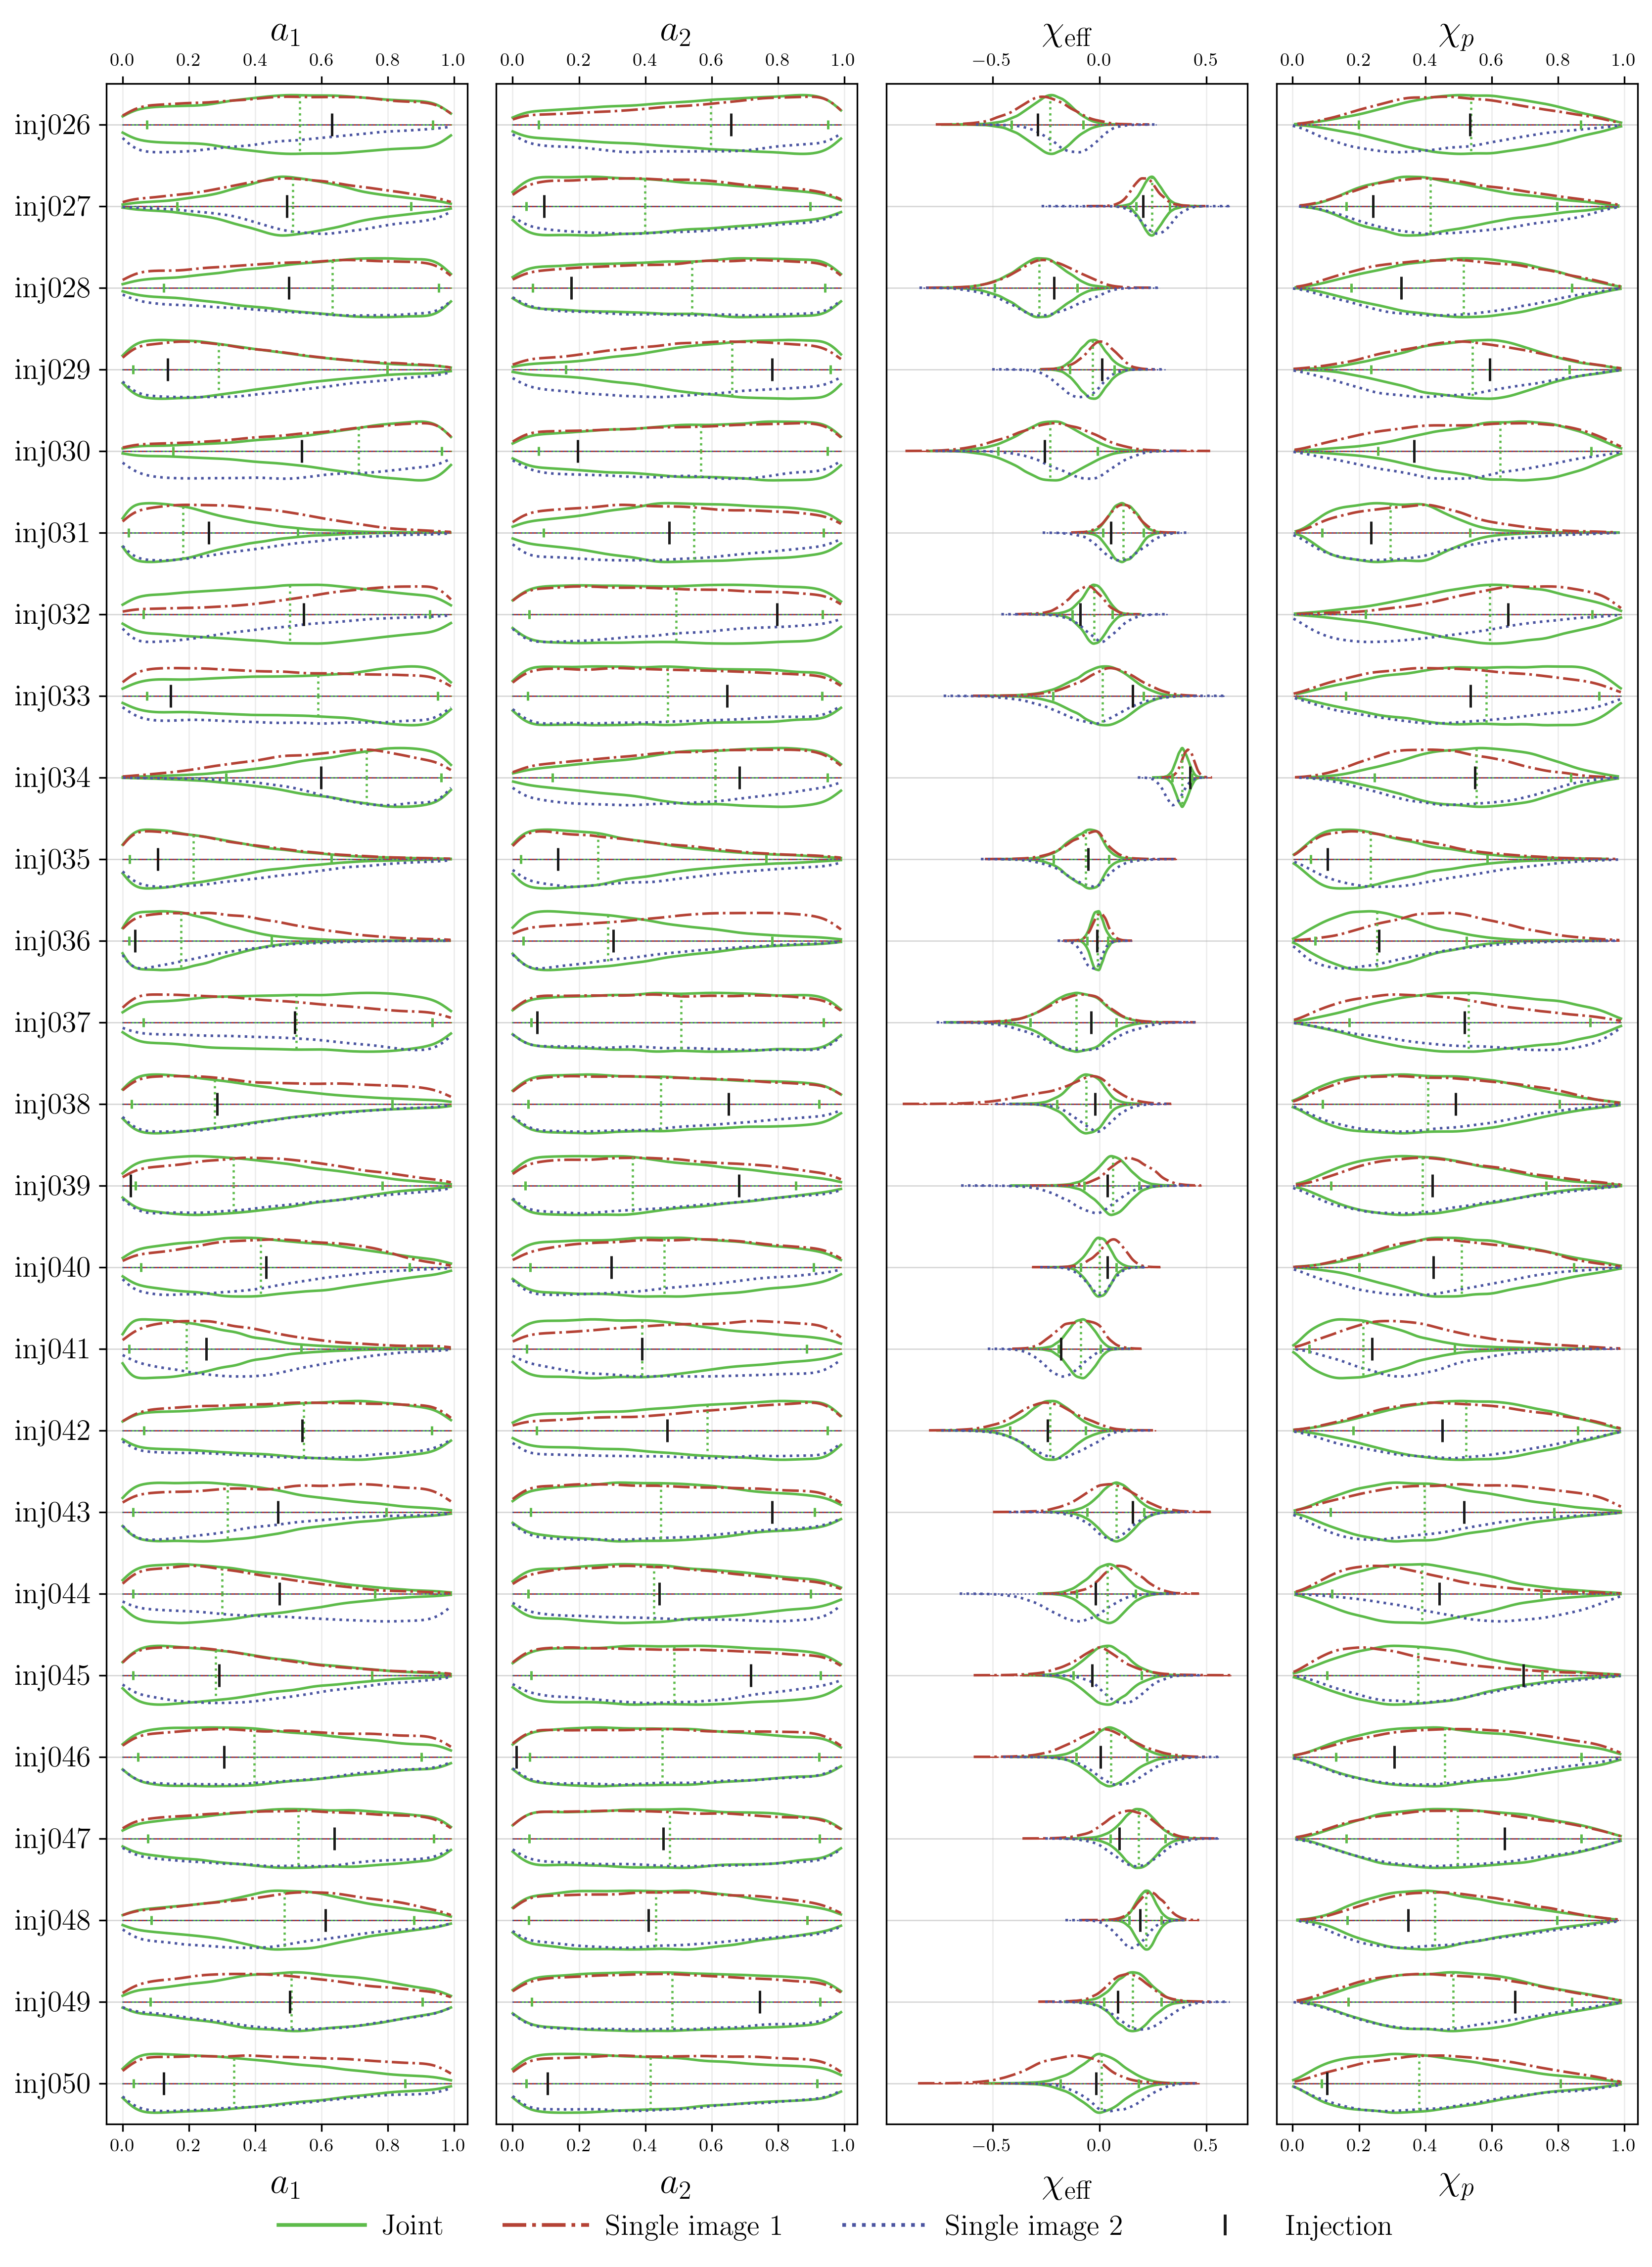
\includegraphics[height=0.92\textheight]{Figures/violin_spins_p02.png}
    \caption[]{Recovered posteriors of $a_1$, $a_2$, $\chi_\mathrm{eff}$, and $\chi_\mathrm{p}$ (2 of 5).}
\end{figure}

\begin{figure}[p]
    \ContinuedFloat
    \centering
    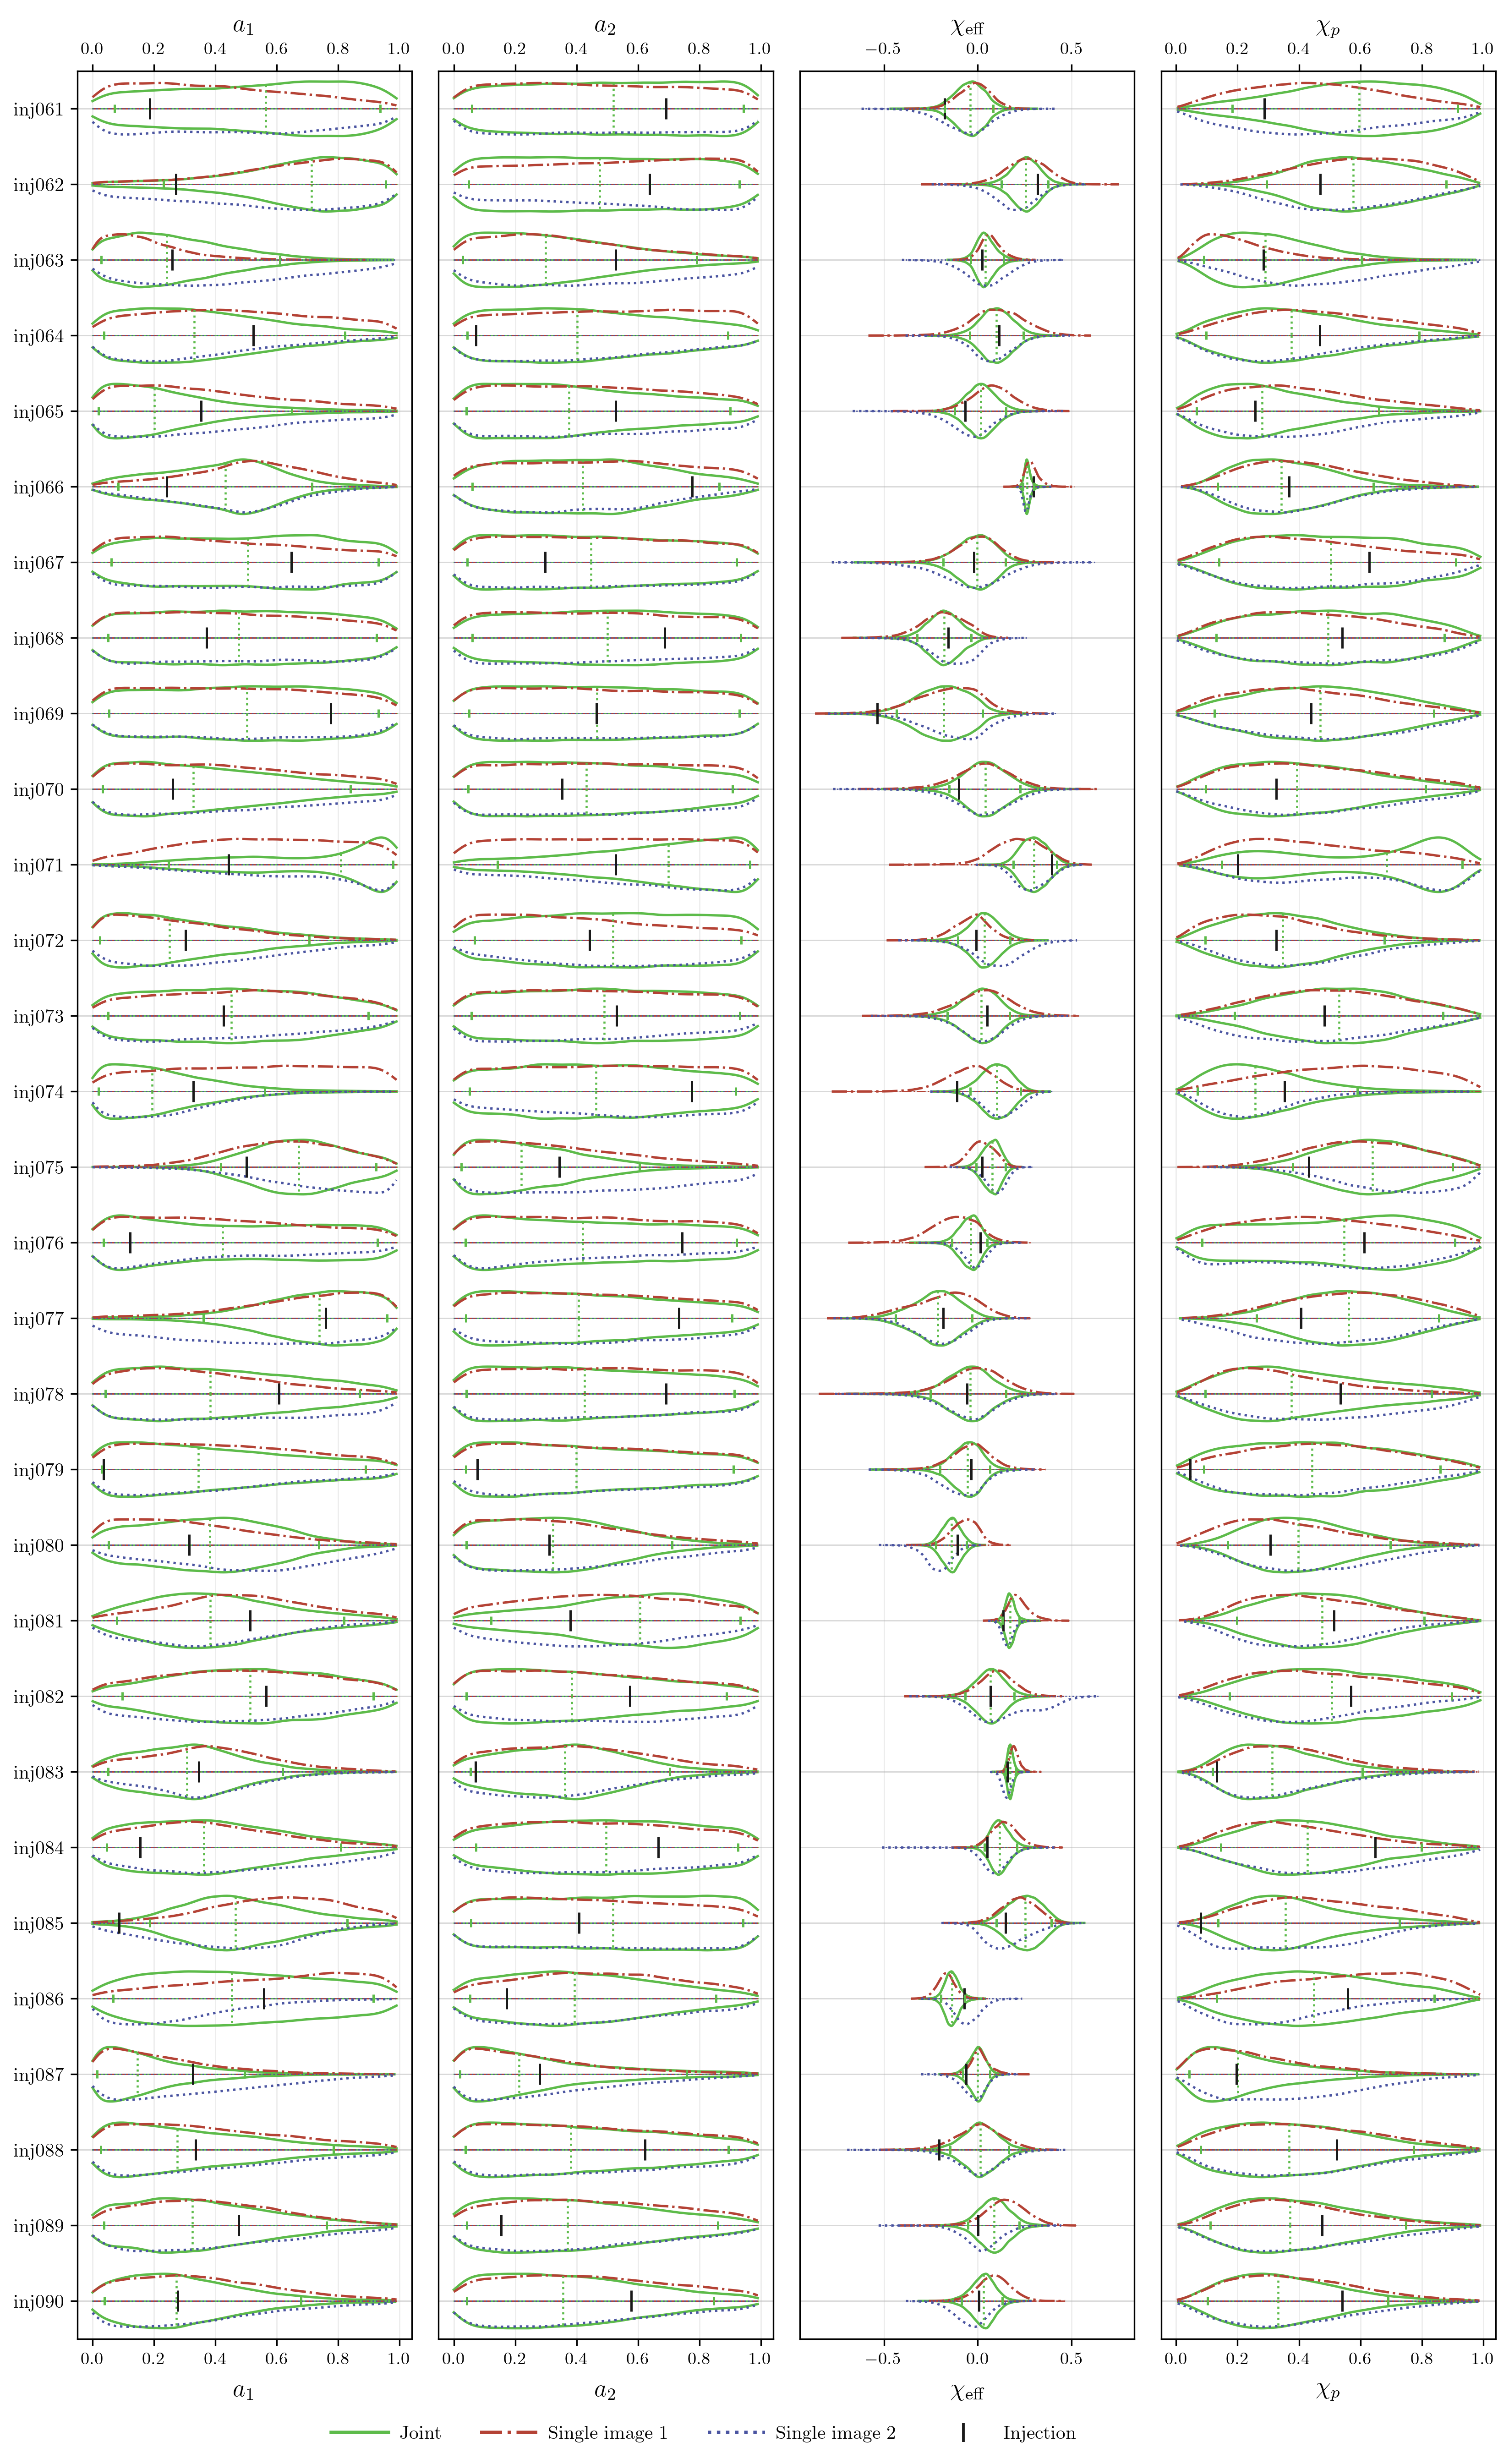
\includegraphics[height=0.92\textheight]{Figures/violin_spins_p03.png}
    \caption[]{Recovered posteriors of $a_1$, $a_2$, $\chi_\mathrm{eff}$, and $\chi_\mathrm{p}$ (3 of 5).}
\end{figure}

\begin{figure}[p]
    \ContinuedFloat
    \centering
    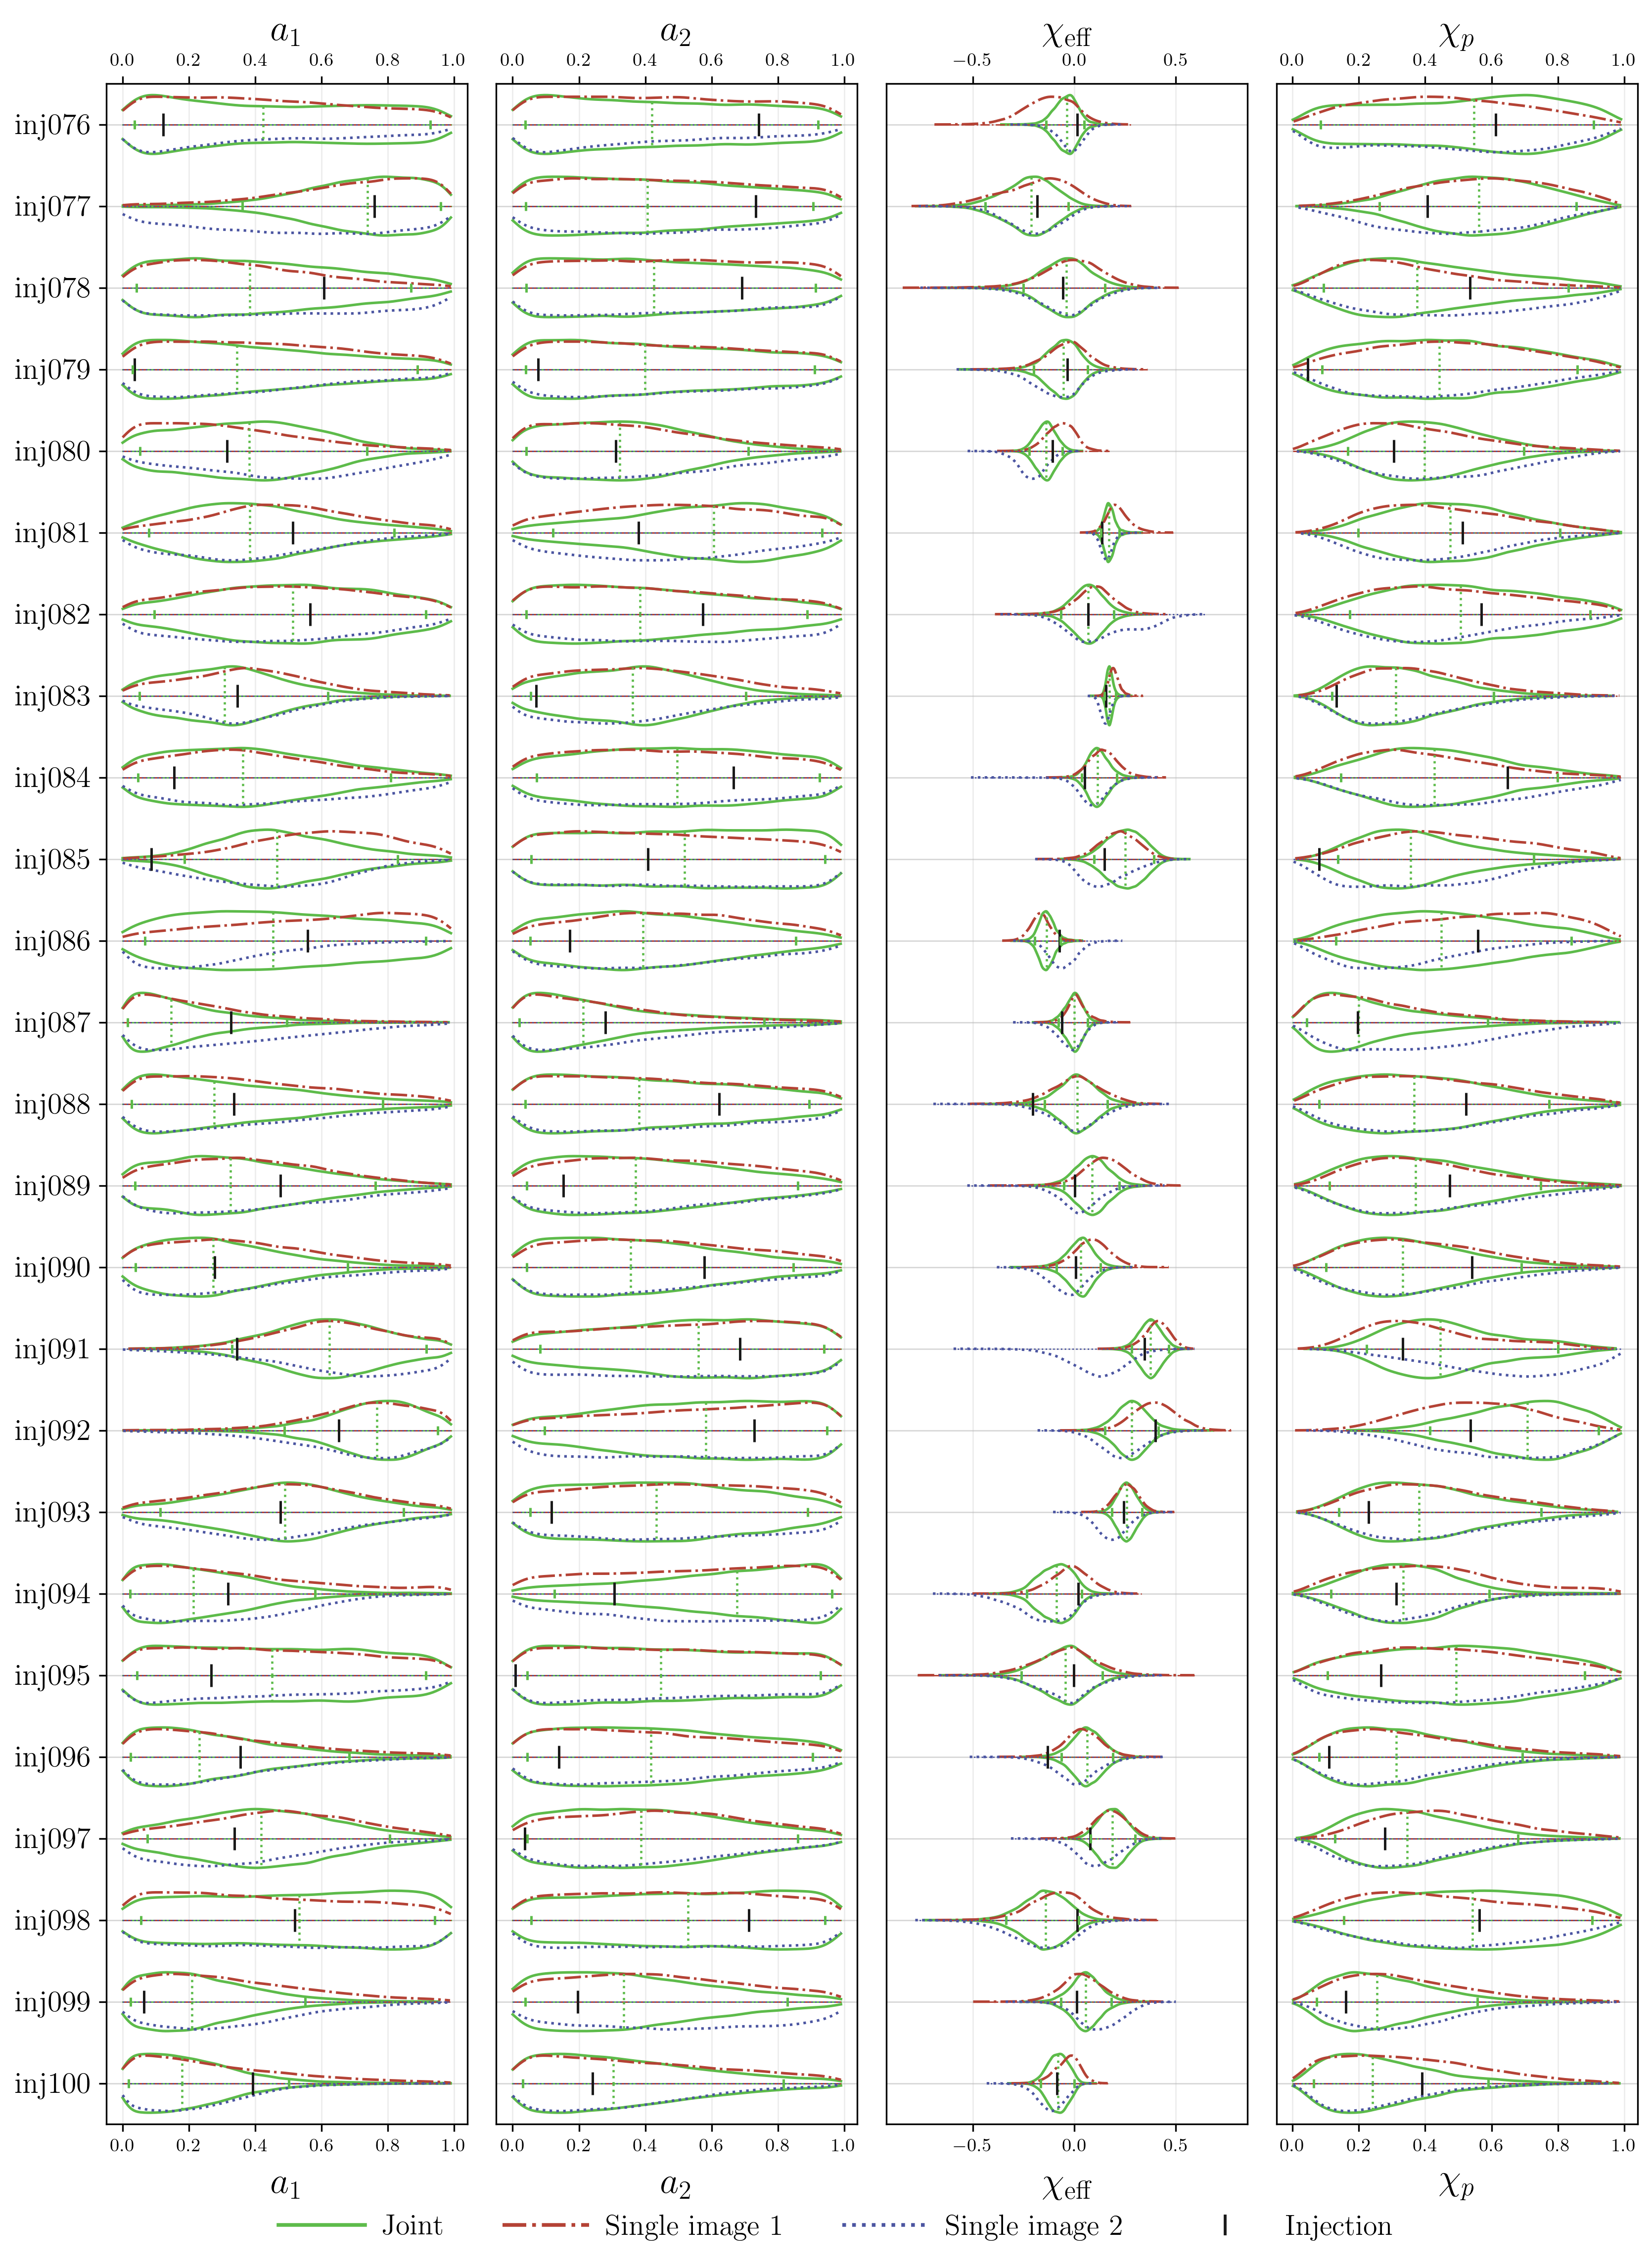
\includegraphics[height=0.92\textheight]{Figures/violin_spins_p04.png}
    \caption[]{Recovered posteriors of $a_1$, $a_2$, $\chi_\mathrm{eff}$, and $\chi_\mathrm{p}$ (4 of 5).}
\end{figure}

\begin{figure}[p]
    \ContinuedFloat
    \centering
    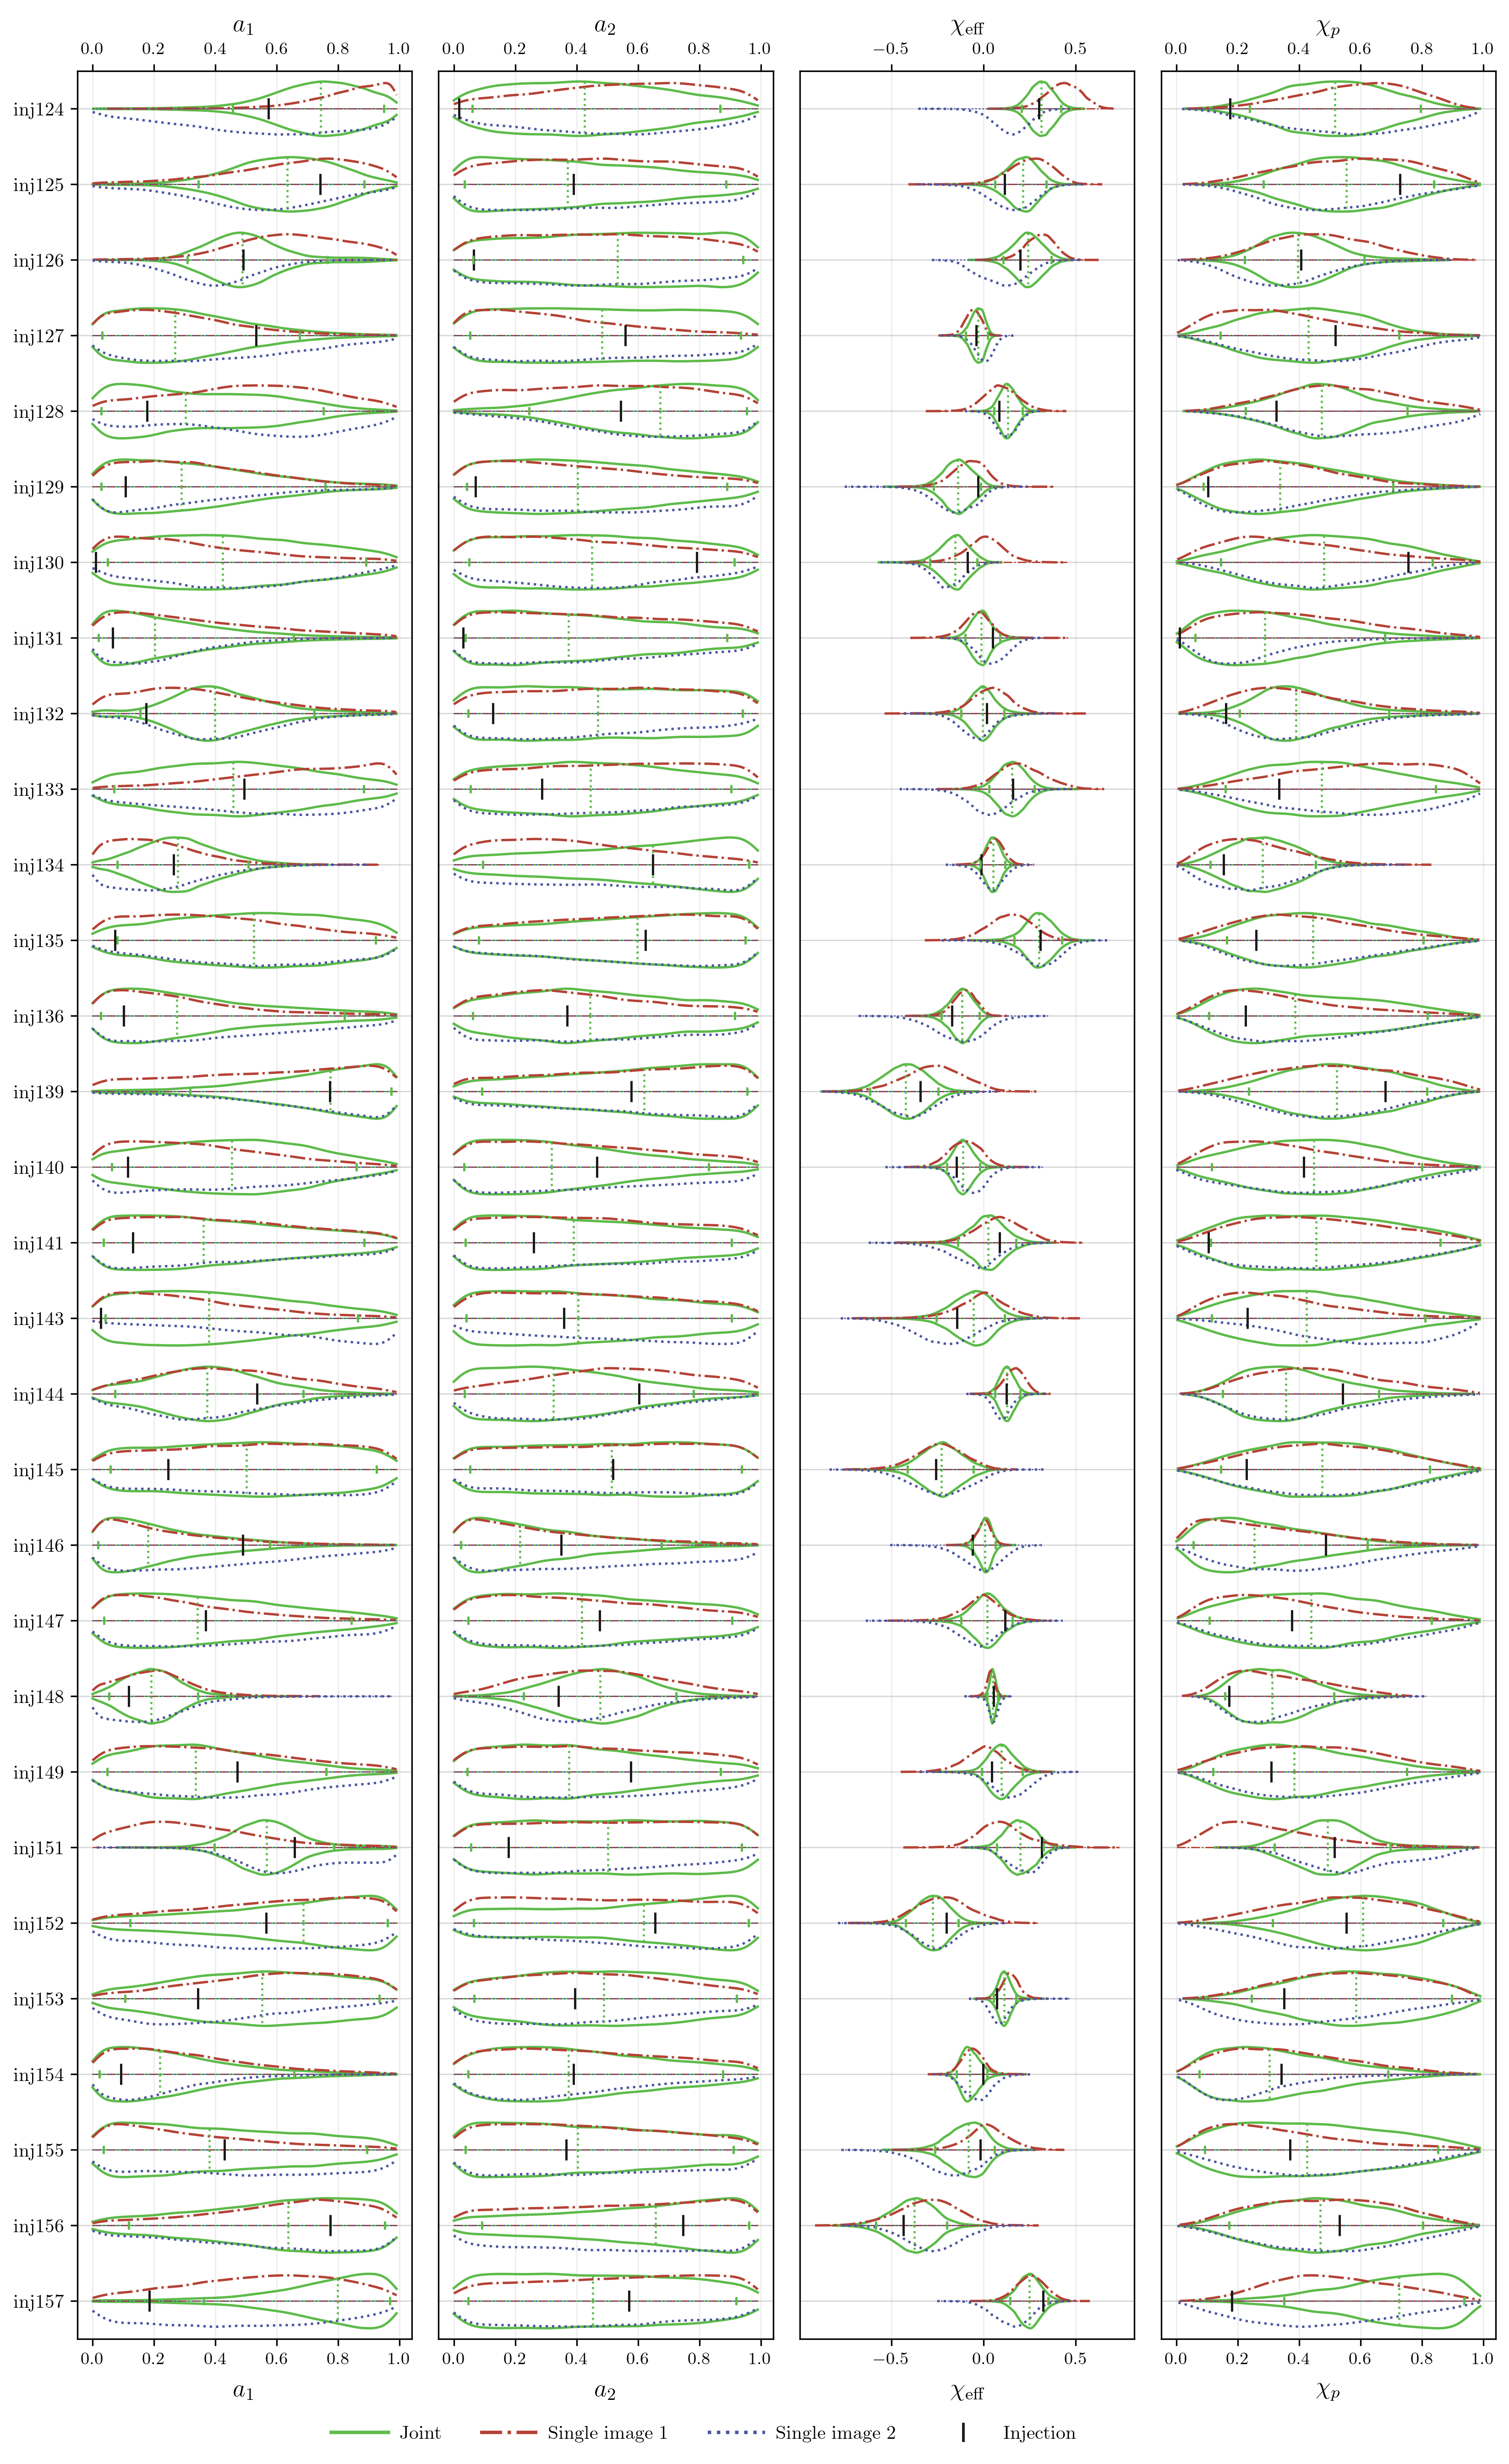
\includegraphics[height=0.92\textheight]{Figures/violin_spins_p05.png}
    \caption[]{Recovered posteriors of $a_1$, $a_2$, $\chi_\mathrm{eff}$, and $\chi_\mathrm{p}$ (5 of 5).}
\end{figure}


\end{document}
